%%%%%%%%%%%%%%%%
% Ph.D. Thesis %
%%%%%%%%%%%%%%%%

%% >> Document Class
% USE THIS FOR DOUBLE SIDED
    %\documentclass[11pt,openright,twoside,letterpaper,onecolumn]{report} 
%% USE THIS FOR SINGLE SIDED
\documentclass[11pt,openright,oneside,letterpaper,onecolumn]{report}  

%% >> Document Formatting
% Holds formatting for document and 
% Title Page, Copyright Page, and Abstract layout
% Change Name/Year/Thesis Title here
% !TEX root = ../main.tex
%%__________________
%% Title, Name, Date
%%------------------
\newcommand{\thesistitle}{A search for new diboson resonances in the boosted semi-leptonic final state at $\sqrt{s} = 13$ TeV with the ATLAS detector}
\newcommand{\thesisauthor}{Ryne Carbone}
\newcommand{\thesisyear}{2017}

%%__________________
%% Packages
%%------------------
%\usepackage[dvips]{epsfig}   % for using dvi
%\usepackage[usenames,pdftex,dvipsnames]{xcolor}
\usepackage[usenames,dvipsnames]{xcolor}
%\usepackage[pdftex]{graphicx} % for includegraphics, otherwise try epsfig
\usepackage{amsmath}  % Need this for math in the title ..
\usepackage{amssymb} % more math symbols
\usepackage{bm} % bold math symbols
\usepackage{fancyhdr}
\usepackage{afterpage}
\usepackage{float} % make float listen for once
\usepackage{cite} % for making ranges
\usepackage{notoccite} % don't use caption citations for numbering
\usepackage{pdflscape}  % If this causes issues, try just lscape
\usepackage{soul}
\usepackage{xargs}            % use more than one optional parameter in a new command
%\usepackage[colorinlistoftodos,textsize=tiny]{todonotes} %mark todo notes (prepend caption disabled)
\usepackage{wrapfig}
\usepackage{fontspec} % for utf-8 with lualatex
\usepackage{tikz-feynman} % Feynman diagrams
\usepackage{xspace}
\usepackage{setspace}
\usepackage[textfont=singlespacing]{caption}
\usepackage{subfig}
%\usepackage{subcaption}
%Styles
\usepackage{sty/atlasmisc}
\usepackage{sty/atlasparticle}
\usepackage{sty/atlasunit}
\usepackage{sty/atlasxref}




% Include hyperref last!!
% We use the hyperref package and customize it for optimal PDF 
%\@thesisauthor
%\@thesistitle
\usepackage[driverfallback=dvipdfm,pdftex,pdftitle={A search for new diboson resonances in the boosted semi-leptonic final state at $sqrt(s) = 13$ TeV with the ATLAS detector},pdfauthor={Ryne Carbone},pdfpagemode={UseOutlines},bookmarks,bookmarksopen=true,pdfstartview={FitH},bookmarksnumbered=true,hyperfootnotes=true]{hyperref}




%%__________
%% Margins
%%----------
\paperwidth=8.5in
\paperheight=11in

%% >> Horizontal margins
% 1in + hoffset + oddsidemargin + textwidth + marginparsep + marginparwidth
% For PhD at Columbia we have single side theses and 1.5in left margin
% The settings below leave 1.5 inch margin at the left and 1 inch at the right 
% for US Letter paper
\setlength{\hoffset}{0.0in}
%\setlength{\oddsidemargin}{.5in} % spaceing from template -- left has extra 0.5margin (maybe for printing purposes)
\setlength{\oddsidemargin}{0.25in} % equal left/right margins (should be 1.25 in
\setlength{\textwidth}{6in}
%\setlength{\evensidemargin}{0.0in} % spacing from template
\setlength{\evensidemargin}{0.25in} % maybe make it equal?

%% >> Vertical Margins
% 1in + voffset + topmargin + headheight + headsep + textheight + footskip 
% For PhD thesis we also need an extra inch at the bottom
% 1inch = 72 pt
\setlength{\voffset}{0.0in}
\setlength{\topmargin}{.0in}
\setlength{\headheight}{14pt}
\setlength{\headsep}{22pt}
\setlength{\textheight}{8.5in}
\setlength{\footskip}{0pt}

%%_________
%% Spacing
%%---------
\renewcommand{\singlespace}{\renewcommand{\baselinestretch}{1.15} \small \normalsize}
\newcommand{\oneandhalfspace}{\renewcommand{\baselinestretch}{1.3} \small \normalsize}
\renewcommand{\doublespace}{\renewcommand{\baselinestretch}{1.5} \small \normalsize}
\newcommand{\normalspace}{\doublespace}
\footnotesep=1\baselineskip

%%_______________
%% Counters depth
%%---------------
\setcounter{secnumdepth}{3}
\setcounter{tocdepth}{3}

%%______________________________
%% Add more space in LOF and LOT
%% Was overlap for 4 digits (e.g. Fig 10.12)
%%_____________________________
\makeatletter
\def\l@figure{\@dottedtocline{1}{1.5em}{3em}}
\def\l@table{\@dottedtocline{1}{1.5em}{3em}}
\makeatother

%%_________________
%% Link Colors
%%-----------------
\hypersetup{
    colorlinks = true, % false: boxed links, true: colored links
    linkcolor  = Maroon,  % internal links
    citecolor  = blue, % links to bib
    urlcolor   = blue, % external link
}

%%____________________
%% Todo notes config
%% hlfix   (red, yellow highlight)
%% Change  (red)
%% Info    (green)
%% Improve (plum)
%% MissingFigure \missingFigure
%%--------------------
%\newcommandx{\hlfix}[3][2=]{\texthl{#1}\todo[linecolor=red,backgroundcolor=red!25,bordercolor=red,#2]{#3}}
%\newcommandx{\change}[2][1=]{\todo[linecolor=red,backgroundcolor=red!25,bordercolor=red,#1]{#2}}
%\newcommandx{\info}[2][1=]{\todo[linecolor=OliveGreen,backgroundcolor=OliveGreen!25,bordercolor=OliveGreen,#1]{#2}}
%\newcommandx{\improve}[2][1=]{\todo[linecolor=Plum,backgroundcolor=Plum!25,bordercolor=Plum,#1]{#2}}
%\newcommandx{\thiswillnotshow}[2][1=]{\todo[disable,#1]{#2}}  % note you can disable  any of the above types with 'disable'


%%_____________
%% Title page
%%-------------
\newcommand{\thesistitlepage}{
    \normalspace
    \thispagestyle{empty}
    \begin{center}
        \textbf{\LARGE \thesistitle} \\[1cm]
        \textbf{\LARGE \thesisauthor} \\[8cm]
        Submitted in partial fulfillment of the \\
        requirements for the degree \\
        of Doctor of Philosophy \\
        in the Graduate School of Arts and Sciences \\[4cm]
        \textbf{\Large COLUMBIA UNIVERSITY} \\[5mm]
        \thesisyear
    \end{center}
    \clearpage
}

%%_________________
%% Copyright page
%%-----------------
\newcommand{\thesiscopyrightpage}{
    \thispagestyle{empty}
    \strut \vfill
    \begin{center}
        \copyright\, \thesisyear \\
        \thesisauthor \\
        All Rights Reserved
    \end{center}
    \cleardoublepage
}

%%_______________
%% Abstract page
%%---------------
\newcommand{\thesisabstract}{
    \thispagestyle{empty}
    \begin{center}
        \textbf{\LARGE ABSTRACT} \\[1cm]
        \textbf{\LARGE \thesistitle} \\[1cm]
        \textbf{\LARGE \thesisauthor} \\[1cm]
    \end{center}
    % !TEX root = ../../main.tex

A search is presented for new resonances decaying to a pair of boosted Standard Model bosons, $WV$, where the $W$ boson decays leptonically ($W\ra\ell\nu$, with $\ell=e,\mu$) and the other weak boson, $V$ ($V=W,Z$), decays hadronically ($V\ra q\bar{q}'/q\bar{q}$ for $q,q'=u,d,c,s,b$).  The data were collected with the ATLAS detector at the CERN Large Hadron Collider, during the 2015 and 2016 periods of $pp$ collisions, at a center-of-mass energy $\sqrt{s}=13\,\TeV$, and correspond to a total integrated luminosity of $36.1\,\ifb$.  
The hadronic decay of the boosted $V$ boson is reconstructed as a single large-radius jet, and the leptonic decay of the $W$ boson is reconstructed as a lepton and missing transverse energy. The search is sensitive to resonances produced with quark-antiquark fusion, gluon-gluon fusion, and vector-boson fusion.  No significant excesses are observed above the Standard Model background prediction. Upper limits on production cross section times branching ratio to $WV$ are set at a 95\,\% confidence level for selected benchmark signal models. Models of a neutral, narrow scalar boson (spin-0), charged and neutral vector bosons (spin-1) coupling to the Standard Model gauge bosons, and a neutral Randall-Sundrum bulk graviton (spin-2) are considered. The search significantly improves the limits produced in recent searches. 
  % file with actual abstract text
    \cleardoublepage
}

%%_______________
%% Draft
%%---------------
\newcommand{\draft}{
    \renewcommand{\normalspace}{\singlespace}
    \normalspace
    \chapter*{Draft. Version \today} % displays dated draft version
    \clearpage 
}

%%-------------
%% Math mode underline
%%-----------
\newsavebox\MBox
\newcommand\Cline[2][red]{{\sbox\MBox{$#2$}%
  \rlap{\usebox\MBox}\color{#1}\rule[-1.2\dp\MBox]{\wd\MBox}{0.5pt}}}


%% >> Start Document
\begin{document}


%%___________________________
%% Title, Copyright, Abstract
%%---------------------------
% For the first pages we do not have numbering 
\pagestyle{empty}

\thesistitlepage
\thesiscopyrightpage
\thesisabstract


%%___________________________________________________
%% Table of Contents, List of Figures, List of Tables
%%---------------------------------------------------
% In the "roman-numbered" section of the thesis, we have numbers at the bottom
% and we have to reduce the text height of the text to make space for the number
\pagenumbering{roman}
\pagestyle{plain}

\setlength{\footskip}{0.5in}

\setcounter{tocdepth}{2}
\renewcommand{\contentsname}{Table of Contents}

%%__________________
%% TABLE OF CONTENTS
%%------------------
\tableofcontents
\cleardoublepage                     % allows next section to jump correctly

%%_________________
%% LIST OF FIGURES
%%-----------------
\listoffigures
\cleardoublepage                     % allows next section to jump correctly

%%________________
%% LIST OF TABLES
%%----------------
\listoftables 
\cleardoublepage                     % allows next section to jump correctly

%%_________________
%% ACKNOWLEDGEMENTS
%%-----------------
\phantomsection \label{sec:ack}      % need this to jump to correct location
\addcontentsline{toc}{chapter}{Acknowledgements}
% !TEX root = ../../main.tex
~\\[1in] % hack to put space at top.
\textbf{\Huge Acknowledgments}\bigskip

\noindent 

Without the comprehensive support and guidance I have received leading up to and during my tenure at Columbia, this thesis would never have been possible. I have been fortunate to have such an extensive network of people assisting me on my journey, and I offer my most sincere gratitude to all of them. 

I want to especially thank my advisor, John Parsons, for his unwavering support through both my studies and research as a graduate student. While enabling me to pursue my interests, he offered a steady hand to lead me through this challenging endeavor. Through his encouragement, guidance, and insights he has made this work possible, and has set an excellent example as a researcher, and mentor.
I want to extend my thanks to the rest of the Columbia ATLAS group, particularly Gustaaf Brooijmans who freely offered aid and advice. 

Without the endless, selfless help of Kalliopi Iordanidou, from debugging code to navigating bureaucracy to deciphering theory, I can candidly say this work would not have been possible; and so to her I would like to show my deepest appreciation. Despite her many responsibilities, she always found time to offer assistance, share her experiences, and help me keep perspective. I want to express my gratitude to the entire $\ell\nu qq$ team, whose tireless work is the basis of this thesis. I want to thank Ismet Siral for the many fruitful conversations on our tram rides back to Geneva.  

During my first summer of research at Nevis Laboratories, Tim Andeen invested countless hours of support and direction, for which I am sincerely thankful. While completing my service work, the entire ATLAS LAr Operations team was welcoming and patient. I want to thank them for their trust, and for the incredible opportunity to work up-close with the detector and its operation. I express my gratitude to my undergraduate advisor, Matthew Herndon, who helped tremendously in cultivating my interest in particle physics.

I want to thank my friends at Columbia for the many shared experiences, somehow surviving coursework and quals: Felix Clark, Laura Havener, Matt Anthony, Zach Greene. I especially want to thank Russell Smith, who also transplanted to Geneva, for the countless discussions, beers, and slopes. I want to thank my friends in Geneva who made my stay enjoyable: the entire Coulou for adopting me as one of their own, and Martin Adams, Daniel Fazio, Nico Hafner, and Jan Stypka for the many hikes, cheese markets, and adventures. I want to thank my friends from Wisconsin, Stuart Frazier, Chris Pom, Arjun Adusumilli, and Monica Cooley who always reminded me where home truly is, even as we spread out. 

I am deeply grateful for Karoliina Lohiniva: you ground me when I need it the most, and are the most understanding, caring, and thoughtful person I know.  

Finally, I want to express my warmest thanks to my family, in particular my parents, John and Velta, and my sisters, Cheyanne and Kailey. You have inspired me to pursue my dreams, and have afforded me every opportunity to succeed. You have shaped me into the person I am today. 



\cleardoublepage                     % allows next section to jump correctly

%%_________________
%% DEDICATION
%%-----------------
% Vertically centered text
\thispagestyle{plain}
\strut \vfill
\centerline{
    \LARGE 
    To my parents,
}
\centerline{
    \LARGE 
    John and Velta
}
\vfill \strut
\cleardoublepage                     % allows next section to jump correctly

%%__________
%% FORWARD
%%----------
\phantomsection \label{sec:forward}  % need this to jump to correct location
\addcontentsline{toc}{chapter}{Foreword}
% !TEX root = ../../main.tex
~\\[1in] % hack to put space at top.
\textbf{\Huge Foreword}\bigskip

\noindent 
%%%
%\iffalse
%%%

%% >> Arriving to NY as graduate student
In the fall of 2012, I joined the Columbia University Physics Department as a graduate student in New York. For the first two years of the program, I took classes and instructed undergraduate courses. 
%% >> Begin research with ADC
My first research experience took place during the summer of 2013 at Nevis Laboratories in Irvington, NY. I contributed to the testing of the Nevis12 ADC~\cite{Nevis12_paper}, a custom integrated circuit designed to meet the requirements
%\footnote{The ADC should be radiation hard (both total ionizing dose and single event effects), dynamic range of approximately 12 bits, latency $<$ 200 ns, sampling at 40 MHz and have power consumption $<$145 mW/channel.} 
for the new trigger electronics in the Liquid Argon (LAr) calorimeter Phase-I Upgrade to the ATLAS detector.
%\footnote{The LAr Phase-I upgrade is scheduled to take place during the second Long Shutdown (LS2) in 2018 to provide higher granularity and higher-resolution, moving the architecture from ``Trigger Towers" to ``Super Cells".} 
%The Nevis12 chip is a dual-channel 12-bit ADC including 4 stages of 1.5-bit(3 outputs) Multiplying Digital to Analogue Converters (MDAC), which allow for digital error correction. I helped create and implement an automated procedure to calibrate the MDACs. 
The Nevis12 chip is a dual-channel 12-bit ADC with digital error correction. I helped create and implement an automated calibration procedure, with which it was possible to quickly characterize the performance of the prototype chips, and measure the Effective Number of Bits (ENOB). In order to verify the radiation hardness, we submitted the Nevis12 chips to radiation testing at Massachusetts General Hospital using their proton beam. The automated calibration procedure allowed for remote recalibration during irradiation, in order to accurately measure the ENOB as a function of dose, and to monitor the stability of the calibration constants. 

%% >> Work with LAr Operations
%% >> noisy cell application
Upon finishing coursework, I relocated to Geneva, Switzerland in June of 2014 to begin full-time research at the CERN Large Hadron Collider (LHC), with the ATLAS experiment. Graduate students working with the ATLAS Experiment are required to perform a body of ``service work'' which aides in the improvement and continuation of the experiment. To satisfy this requirement, I joined the LAr calorimeter operations team, and originally focused on improving the online software. During my time with the online team, I created and developed an automated application which monitors electrically noisy calorimeter cells during data taking, and makes decisions about disabling the cells if the noise level is persistently high. %Electrically noisy cells contribute to an overestimation of deposited energy. 
During the previous LHC run (Run-1), this process was done manually by on-call experts. Often, coordination between multiple groups was required to retrieve all of the appropriate information. Furthermore, it is only possible to identify groups of cells which could be responsible for the increased noise, so experts were required to use trial and error in a tedious, time-consuming manner. The current application pools together the rate information automatically, queues commands to disable cells in the noisy region, and evaluates the effect of disabling a given cell in a quick, systematic procedure. The shifter in the ATLAS control room is able to monitor all of the actions, and notify the on-call expert in case additional help is needed, greatly reducing the overall workload. 

%% >> Run Coordinator
After gaining hands-on experience with the online team and familiarizing myself with the LAr calorimeter operations, I took on greater responsibilities by serving as a LAr Run Coordinator. As Run Coordinator, I was required to be ``on-call'' around the clock for week-long shifts. A Run Coordinator is responsible for leading the operations of the subdetector: they head daily subdetector meetings to prioritize and plan the schedule, they present the status of the subdetector at daily ATLAS meetings, they coordinate tests and calibrations with other subsystems, they coordinate when hardware interventions are to be executed, and they are in contact with the shifters in the ATLAS control room and the LAr on-call team. The Run Coordinator is the first contact in case of any problems reported from the control room, and is responsible for quickly deciding the seriousness of the issue, how to resolve it, and who must be contacted. 

%% >> Work with Online Timing
Upon completion of my service work, I began interacting more closely with the diboson resonance analysis team, the search on which this thesis is based.
However, I continued contributing to LAr efforts. I was given the chance to present the status and performance of the LAr calorimeter during 2015 proton collisions at the 2016 LHCC meeting~\cite{lhcc_poster}. I was also asked to present a talk concerning the Phase-I and Phase-II upgrades of the LAr calorimeter at ICHEP in 2016~\cite{ryne_ichep_talk}. I performed additional studies for the LAr calorimeter by measuring and analyzing both the online and offline timing performance. Working with Kalliopi Iordanidou, we used 2015 $pp$ collision data to measure and provide corrections to the Front-End Board (FEB) fine-delays, in order to synchronize the online timing. In each subdetector of the calorimeter, the FEB timing showed excellent alignment: Gaussian fits yielded mean values well below 1 ns\footnote{
    0 ns corresponds to a highly relativistic particle originating from the center of the detector.
} and RMS values around 0.2 ns~\cite{LArCaloPublicResults2015}. FEB timing below 1 ns ensures accurate energy reconstruction.
%\footnote{The sets of coefficients used to calculate the energy from the signal pulse samples are derived in bins of 25/24 ns, hence online timing better than $\sim$1 ns has a negligible effect on the energy.}. 

%% >> Work with Offline Timing
Following a study of 2011 and 2012 $pp$ data done by a previous Columbia student, Nikiforos Nikiforou, 
%~\cite{LArTiming_2012}, 
I optimized the calorimeter offline timing performance for the 2015 $pp$ data~\cite{LArTiming_2015}. A seven-step calibration procedure was used to significantly improve the time resolution and synchronization of the LAr calorimeter. Among other effects, the calibration takes into account energy dependence, cross-talk effects, and variations between runs. In the end, average calorimeter cell times centered to 0 ns from original offsets of $500-900$ ps, and time resolution improved from approximately $500-800$ ps to $200-270$ ps. Sub-nanosecond time resolution is important for various exotic physics searches involving long-lived neutral particles. To facilitate these searches, I coded a tool that applies the precision offline timing corrections derived from the study. Additionally, the tool can smear the timing of Monte Carlo generated events to match the measured time resolution in the detector. Notably, I utilized this tool in a cross-check study of the timing correlation between photons in the 2015 diphoton resonance search~\cite{diphoton_paper}.

This thesis is based on the analysis in~\Ref{\cite{finalpaperlvJ}}, which is entering the final stages of review within ATLAS, and will be submitted to the Journal of High Energy Physics later this year. The analysis searches for new resonances decaying to a pair of SM bosons, where one daughter boson decays to a lepton and neutrino, and the other decays to a pair of quarks. This thesis focuses on the boosted regime where the two quarks are highly collimated (approximately for resonance masses above $500\,\GeV$), while the analysis in~\Ref{\cite{finalpaperlvJ}} additionally considers decays where the two quarks can be substantially separated.


%% Todo
%Summer school poster?

%%%
%\fi
%%%







\cleardoublepage                     % allows next section to jump correctly

%%_________________
%%  Draft Version
%%-----------------
%\draft                              % Generates a draft version in single-space

%%____________
%% BODY
%%------------
% In the "arabic" section of the thesis, we do not have numbers at  the
% bottom and we want to use the full length of the page to avoid vbox
% underfulls. We use the fancyheaders package to adapt the headers
% according to the  Columbia requirements.
\pagestyle{headings}
\pagenumbering{arabic}
\setlength{\textheight}{8.5in}
\setlength{\footskip}{0in}

% We change the pagestyle 
\fancypagestyle{plain} {
    \fancyhf{}
    %% These two lines for DOUBLE SIDED
        %\fancyhead[LE,RO]{\thepage}
        %\fancyhead[RE,LO]{\itshape \leftmark}
    %% OR These two lines for SINGLE SIDED
        \fancyhead[R]{\thepage}
        \fancyhead[L]{\itshape \leftmark}
    \renewcommand{\headrulewidth}{0pt}
}
\pagestyle{plain}

%%______________________________
%% PREFACE:
%% Introduction
%% Standard Model, Limitations
%% LHC
%% ATLAS Detector
%%------------------------------
%%__________________________________
%% Intro, Standard Model, 
%% Limitations, LHC, ATLAS Detector
%%----------------------------------

% !TEX root = ../../main.tex
\chapter{Introduction}
\label{ch:intro}

Over the past four decades since the formulation of the Standard Model (SM), the theory has been tested with remarkable precision. 
Combining the theory of electroweak interactions with the theory of strong interactions in the same mathematical framework, the SM describes the physics of particles and fields up to the\,\TeV\, scale. All of the predicted constituents have been observed, culminating with the discovery of the Higgs boson in 2012~\cite{Higgs_atlas,Higgs_cms}.

Despite the success of the SM, it is not a complete theory of the physical universe. Notably, the SM does not incorporate a theory of gravity. Observed phenomena ranging from dark matter (inferred, for example, from the observed rotation curves of galaxies), to neutrino masses (inferred from the measurements of neutrino oscillations), to matter-antimatter asymmetry (the observed, extreme imbalance between the amount of particles and anti-particles in the universe) all indicate extensions of the current theory are needed. Among others, a critical theoretical concern is known as the hierarchy problem. An unsatisfying ``fine-tuning'' in the cancellation of divergent terms in the calculation of the Higgs mass is required to reproduce the observed value. 
% Mention weak vs gravity scale?

This thesis considers several models of new physics which purport to address shortcomings of the SM. Common to all of the theories considered is the prediction of as-yet-undiscovered, massive boson resonances which couple to the SM weak gauge bosons. If the masses of these new resonances are near the\,\TeV\,scale, they are kinematically accessible to searches at the Large Hadron Collider (LHC). Due to their decay to a pair of much lighter weak gauge bosons, the resonances would produce decay products that would be observed in the detector as highly boosted (large momentum) final state particles. 

In this search, the semi-leptonic final state refers to resonance decays where one of the daughter weak bosons decays to a lepton and a neutrino (leptonic decay), while the other decays to a pair of quarks (hadronic decay). For heavy resonances much more massive than the SM weak bosons, the two quarks from the boosted daughter weak boson decay will be highly collimated. The standard distance parameter used to reconstruct hadronic decays as ``jets'' will then be too large to separately distinguish the energy deposits of the two quarks, and too small to completely capture the total energy deposit from both. Consequently, in this search, a larger distance parameter is used to reconstruct the hadronically decaying boson as a single jet. By analyzing the substructure and mass of this jet, effective discrimination can be made between whether it is due to a true decay of a weak boson, or a processes imitating the decay with a similar topology.

% The search method
This thesis uses data collected in 2015 and 2016 with the ATLAS detector~\cite{ATLAS} at the LHC~\cite{LHC}, from $pp$ collisions with a center-of-mass energy $\sqrt{s}=13\,\TeV$, corresponding to a total integrated luminosity of $36.1\,\ifb$.  This search uses the mass distribution of the reconstructed diboson system as a discriminating variable to look for excesses above the SM background predictions. The results of the search are consistent with the SM background predictions. Constraints on the phase space of new physics are presented for selected benchmark signal models, and the results of the most recent searches~\cite{diboson_comb_2016, ATLAS_comb_run1, lvjj_run1, CMS_diboson_run2, CMS_diboson_run1run2, CMS_dijet_run1, CMS_diboson_run1} are significantly extended. The content and organization of this thesis are summarized below. 


% Organization of paper
In~\Ch{\ref{ch:stdmodel}}, a brief discussion of the SM of particle physics is given. The theoretical foundations of selected theories describing physics beyond the SM are given in~\Ch{\ref{ch:limitations}}, with an emphasis on the benchmark signal models considered in this thesis. In~\Ch{\ref{ch:lhc}} and~\Ch{\ref{ch:atlas}}, the experimental setup is outlined, including descriptions of the LHC, and the ATLAS detector, respectively. 
The reconstruction of physics objects from detector measurements in data and simulation is presented in~\Ch{\ref{ch:objreco}}. The strategy of the search is discussed in~\Ch{\ref{ch:analysisStrategy}}, including a discussion on the boosted event topology, the main SM backgrounds, and the methods of modeling signal and background processes. In~\Ch{\ref{ch:event_selection}}, the selection and classification of events in data and simulation are discussed. The signal regions sensitive to new physics, and the control regions used to validate the background modeling, are defined. 
The systematic uncertainties considered in this search are discussed in~\Ch{\ref{ch:syst}}. The statistical methods used to evaluate the results are outlined in~\Ch{\ref{ch:stats}}, and the final results are presented in~\Ch{\ref{ch:results}}. Finally, in~\Ch{\ref{sec:conclusions}} a summary of the search and a few concluding remarks are given.





% !TEX root = ../../main.tex
% !TEX encoding = UTF-8 Unicode
%%%
\chapter{The Standard Model}
\label{ch:stdmodel}

% Inline fraction for text
%\newcommand{\slantfrac}[2]{\,^#1\!/_#2}


The Standard Model (SM) is a quantum field theory describing the elementary particles and fundamental forces (with the exception of gravity)
%\footnote{Except when stated otherwise, discussion of forces in the context of the SM will not refer to gravity.} 
that govern the universe. At its core, the SM states that all matter is composed of fundamental particles called fermions, all forces are mediated by force carrying gauge bosons, and all massive fundamental particles acquire their mass through interactions with the Higgs boson.

The importance of the SM to our understanding of the physical world is reflected in the 17 Nobel Prizes in physics that have been awarded since 1957 for work relating to the development and verification of the SM~\cite{Nobel_Prizes}. That the current theory describes with remarkable accuracy nearly all observed phenomena of electromagnetic, weak, and strong interactions in a compact theory with rich symmetries can belie the tumultuous and often uncertain path that lead to it's development. In this chapter, a brief discussion of the content and formulation of the SM is presented. 

%
\section{Particle Content}

In ~\Fig{\ref{fig:st_m_p}}, the particle content of the SM is succinctly summarized. The particles are elementary: they cannot be decomposed further into smaller constituents. There are two broad categories of particles: fermions (half integer spin) and bosons (integer spin). Spin is an intrinsic property of a particle, and is a form of angular momentum. Fermions and bosons necessarily behave differently according to the Spin-Statistics Theorem\footnote{
	An important consequence of the theorem is the Pauli exclusion principle for fermions: no two fermions can occupy the same quantum state. Bosons have no such restriction, and thus any number can occupy the same quantum state.
}~\cite{spin_stats}. The fermions in the SM are further subdivided into quarks and leptons, while the bosons are subdivided into gauge (spin 1) and scalar (spin 0) bosons. 

\begin{figure}[htb]
\begin{center}
\includegraphics[width=0.7\textwidth]{figures/StandardModel/std_model}
\end{center}
\caption[Fundamental particles in the Standard Model]{A categorization of the fundamental particles in the Standard Model is shown: quarks and leptons together constitute all the matter particles, the gauge bosons mediate the electromagnetic, weak, and strong forces, and the Higgs boson generates mass for the fundamental particles.}
\label{fig:st_m_p}
\end{figure}

All matter is composed of quarks and leptons, which are divided into three generations of increasing mass\footnote{
	The exact mass hierarchy of the neutrinos has not been determined.
}. A generation includes two quarks, one with electric charge $+2/3$ (in units of the fundamental electric charge scale, $e$) and one with $-1/3$, one negatively charged lepton, and one neutral lepton called a neutrino. The particles in different generations mainly differ in their masses. Each fermion has an associated anti-particle with identical properties, with the exception of an inverted electric charge.

The three quarks with electric charge $+2/3$, known as up-type quarks, are called up, charm, and top, and are denoted by u, c, and t, respectively. The three quarks with electric charge $-1/3$, known as down-type quarks, are called down, strange, and bottom, and are denoted by d, s, and b, respectively. Due to the strong force, quarks do not exist in isolation, but rather combine to form hadrons like protons, neutrons, and pions. Hadrons are typically composed of either two quarks (meson) or three quarks (baryon), although a pentaquark state has been recently experimentally verified~\cite{pentaquark}.

In order of increasing mass, the charged leptons are the electron, muon, and tau and are denoted by $e,\mu$, and $\tau$, respectively. The neutrinos are labeled by the charged lepton in their generation: $\nu_e,\nu_{\mu}$, and $\nu_{\tau}$. 
Leptons only interact with the electromagnetic and weak forces, and in contrast to quarks can exist in isolation. The heaviest charged leptons have a finite lifetime and decay to electrons which are stable. Neutrinos have an extremely small, non-zero mass, and oscillate as they propagate through space\footnote{
	The oscillation is a predictable, periodic transformation between the three neutrino generations. Neutrinos are produced in weak eigenstates, e.g. $\nu_e$, which, however, do not correspond to mass eigenstates.
}. 

The gauge bosons mediate the electromagnetic, weak, and strong forces: particles that interact via a certain force do so through the exchange of gauge bosons. The photon has no mass or electric charge, and mediates the electromagnetic force. Since it has no mass, the photon is stable and can propagate through space indefinitely. The weak force is mediated by the $Z^0$, $W^+$, and $W^-$ bosons, where the superscript denotes the electric charge. All three weak bosons are massive, and have a finite lifetime. The gluon is responsible for mediating the strong force. Like the photon, it is massless and has no electric charge; however, it has an analogous ``color charge'' associated with the strong interaction. 

Finally, the Higgs boson is a massive scalar (spin-0) particle with no electric charge. Through a process called the Higgs mechanism, it is responsible for generating masses of the fermions, weak gauge bosons, and itself.  


%
%%%
\iffalse
%%%
\section{Arriving at the Standard Model}

Our current understanding of the fundamental interactions between elementary particles is derived from this astonishingly nascent theory. In the span of 13 years, the SM in its current form was developed. In 1961, Glashow first proposed a way to combine the electromagnetic and weak interactions~\cite{Glashow:1961tr}; in 1967, Weinberg and Salam independently incorporated the Higgs mechanism~\cite{Weinberg,Salam:1968rm}; and by 1974, quantum chromodynamics (QCD) with the inclusion of asymptotic freedom~\cite{Gross_Wilczek, Politzer} rendered the basic form of the current Standard Model\footnote{
	There would still be much to verify and refine, such as the number of leptons and quarks, but the pillars of the theory were formed. 
}. 

A mere 64 years prior to Glashow's electroweak proposal, the {\em first} fundamental particle was discovered by J.J. Thompson in 1897: the electron\footnote{
	The celerity with which this feat has been achieved is reminiscent of the 66 years separating the Wright brothers' initial flight (1903) and the Apollo 11 moon landing (1969), coincidentally transpiring nearly contemporaneously.
}. By 1911 Rutherford had discovered the nucleus and in 1913 the primitive Bohr model gave accurate predictions for Hydrogen energy levels. Even during this relatively simple period, there were hints of a coming quantum model: in 1905 Einstein's photoelectric effect unequivocally demonstrated the existence of the massless photon. 

With the advent of quantum mechanics in 1925, the picture of fundamental particles began to expand. In 1928 Dirac postulated the existence of the positron\footnote{
	He recognized his equation permitted negative energy electron solutions.
}, in 1930 Pauli theorized the neutrino to conserve energy in $\beta$ decays, and in 1935 Yukawa theorized nuclei were held together by a nuclear force through the exchange of mesons.  

In 1947, most of the predicted particles had been found\footnote{
	The muon was not predicted, but found nonetheless, while the neutrino would't be found until later.
}, however the discovery of a new meson, the kaon, would spark another revolution in the theory of elementary particles. In the following decade, a ``zoo'' of new mesons and baryons were discovered, and physicists struggled to find a way to neatly classify them. Finally in 1961, Gell-Mann introduced the Eightfold Way to describe the symmetries of mesons and baryons as representations of the group SU(3). The power of this classification of symmetries was immediately evident when the $\Omega^-$ baryon predicted by the theory was discovered in 1964. In the same year, Gell-Mann and Zweig proposed the quark model which codified the symmetries of the Eightfold Way with three quarks and anti-quarks that combined to form mesons and baryons. The use of group theory to classify the interactions of elementary particles in terms of symmetries would drive the development of the field, resulting eventually in the current theory of the SM.

%%%
\fi
%%%

%
\section{Formulation of Symmetries}
The principle of least action with a Lagrangian density is used to describe the propagation and interactions of quanta and fields: for an arbitrary field $\phi$, obeying the equations of motion described by the Lagrangian density, $\mathcal{L}(\phi,\partial \phi)$, the action is defined as:
 $$S[\phi] = \int d^4x \mathcal{L}(\phi(x),\partial\phi(x)); \quad\quad \delta S = 0$$ 
 According to Noether's Theorem, for every continuous global symmetry of the action, there is an associated conserved charge~\cite{noether}. For local gauge symmetries, an equation of motion for generated gauge fields is produced.

The group corresponding to all Poincar\'e transformations characterizes the 10 global continuous symmetries of special relativity; translations in space and time (four), rotations in space (three), and boosts in space (three)~\cite{Srednicki}. As a relativistic quantum field theory, the SM incorporates special relativity; hence, the Poincar\'e symmetry is a global continuous symmetry of the theory. Associated with this global symmetry are three conserved quantities: energy, momentum, and angular momentum.  In the SM, spin-0 particles are described by scalar fields, $\phi$, obeying the Klein-Gordon equation, spin-$1/2$ particles are described by spinor fields, $\psi$, obeying the Dirac equation, and spin-1 particles are described by vector fields, $A_{\mu}$, obeying the Proca equation.

To impose a specific symmetry on the theory, the goal is to derive a Lagrangian which is invariant under the corresponding transformations. Often these are continuous symmetries which can be thought of as abstract rotations of the fields. As an example, consider the free spinor field obeying the Dirac equation:
$$\mathcal{L}=\bar{\psi}(\gamma^{\mu}\partial_{\mu}-m)\psi$$
This is invariant under the global transformation $\psi(x)\ra\psi'(x)=e^{i\alpha}\psi(x)$. The continuous symmetry is characterized by its infinitesimal behavior near the identity transformation. In group theory, this symmetry is characterized by the Lie algebra of U(1), for which there is one generator, $\alpha$~\cite{wukitung}. If $\alpha$ is a function of space-time, the derivative in the Lagrangian produces an extra term. To retain invariance, a covariant derivative can be introduced:
$$\partial_{\mu}\rightarrow D_{\mu} = \partial_{\mu} - ieA_{\mu}$$
where $e$ describes a coupling, and the gauge field, $A_{\mu}(x)$, transforms as:
$$A_{\mu}(x)\ra A'_{\mu}(x)=A_{\mu}(x)+ \frac{1}{e}\partial_{\mu}\alpha(x)$$
Finally, a term corresponding the the free propagation of this new massless gauge field is added to the Lagrangian.

This process of identifying a global symmetry of free fields and requiring it to also be a local or gauge symmetry is the general process through which the interactions in the SM are constructed. For each underlying local symmetry there are generators which form a basis for the Lie algebra describing it, and for each generator a gauge field must be introduced to preserve the symmetry. The gauge fields couple to the original fields and determine the interactions of the theory. The resulting theory is known as a gauge theory which, as shown by 't Hooft, implies the theory is renormalizable~\cite{thooft}. The full local gauge symmetry of the SM is described by the group $SU(3)\times SU(2)_L\times U(1)_Y$ which describes the strong and electroweak interactions~\cite{Griffiths, Srednicki}.

%
\section{Electroweak Sector}
The electroweak interaction preserves the internal weak isospin and weak hypercharge symmetries corresponding to the group $SU(2)_L\times U(1)_Y$. The subscript $L$ indicates that the weak isospin $SU(2)$ symmetry is restricted to left-handed fields, while the subscript $Y$ corresponds to the weak hypercharge which generates the U(1) symmetry. The electroweak interaction is thus described by a chiral theory since it couples differently to left-handed and right-handed fields, which are defined by how they behave under Lorentz transformations.

The restricted Lorentz group is a subgroup of the Poincar\'e group corresponding to the generators of boosts and rotations. These six generators can be rearranged into a direct sum of two Lie algebras corresponding to the group $SU(2)\times SU(2)$~\cite{Srednicki}. A fermion field can be expressed as a Dirac spinor in the $(\frac{1}{2},0)\oplus(0,\frac{1}{2})$ representation of the restricted Lorentz group as $\Psi = \begin{pmatrix}\psi_L\\\psi_R\end{pmatrix}$, where $\psi_L$ and $\psi_R$ are left-handed and right-handed Weyl spinors. The left-handed and right-handed spinor components of the Dirac field do not mix under a Lorentz transformation.

The chiral, weak isospin symmetry is maximally parity violating: left handed fermion fields transform as $SU(2)_L$ doublets in the defining representation, while right-handed fermion fields are represented as $SU(2)_L$ singlets in the trivial representation. The lepton and quark fields can be grouped in terms of their chiral components as shown in~\Tab{\ref{tab:ew_rep}}.  There are three generators for the Lie algebra of $SU(2)$; thus, by requiring $SU(2)_L$ to be a local gauge symmetry, three vector gauge fields are introduced in the adjoint representation: $W_{\mu}^1,W_{\mu}^2$, and $W_{\mu}^3$. 

The $U(1)_Y$ weak hypercharge symmetry is not chiral, as it couples to both left-handed and right-handed fields. The weak hypercharge of a field is chosen in a suggestive way: $Y=2(Q-I_3)$, where $Q$ is the electric charge and $I_3$ is the third component of the weak isospin. Corresponding to the single generator of the Lie algebra of $U(1)$, one vector gauge field, $B_{\mu}$, is introduced to ensure the local gauge invariance of the $U(1)_Y$ symmetry. 

\begin{table}[tbp]
\begin{center}
\begin{tabular}{lccc}
\hline\hline
Particle type & SU(2)$_L$ Grouping & Isospin ($I_3$) & Hypercharge (Y) \\\hline
Left-handed leptons &$ \begin{pmatrix} \nu_L \\ e_L \end{pmatrix} $& $\pm\frac{1}{2}$ &$ -1$\\
Left-handed quarks &$ \begin{pmatrix} u_L \\ d_L \end{pmatrix} $& $\pm\frac{1}{2}$ &$ \frac{1}{3}$\\
Right-handed neutrino$^{\dagger}$& $\nu_R$ & 0 & 0 \\
Right-handed electron & $e_R$ & 0 & $-2$ \\
Right-handed up quark & $u_R$ & 0 & $\frac{4}{3}$\\
Right-handed down quark & $d_R$ & 0 &$-\frac{2}{3}$\\\hline\hline
\end{tabular}
\end{center}
\caption[Weak isospin and hypercharge groupings of the electroweak sector]{The weak isospin and hypercharge properties of the first generation of fermions is presented.\\\,$^{\dagger}$Right-handed neutrinos do not interact at all, if they exist. For this reason they are not usually included in the formulation of the SM.}
\label{tab:ew_rep}
\end{table}

The four vector gauge fields $W_{\mu}^i, B_{\mu}$ and all the fermion fields must be massless to preserve the imposed gauge invariance; however, experimentally all fermions have mass, and there are three massive weak bosons and one massless photon. The solution is to introduce a complex scalar field, $\Phi=\begin{pmatrix}\phi^+\\\phi^0\end{pmatrix}$, which is a weak isospin doublet with hypercharge $Y=1$, and a potential of the form $V(\Phi) = -\mu^2\Phi^{\dagger}\Phi + \lambda(\Phi^{\dagger}\Phi)^2$, which furthermore respects gauge invariance. By expanding the field about the minimum of the potential, known as the vacuum expectation value $v$, and choosing the unitary gauge so that it is real, the scalar field becomes $\Phi=\frac{1}{\sqrt{2}}\begin{pmatrix}0\\v+H(x)\end{pmatrix}$. The excitation field, $H$, is now interpreted as the physical Higgs field, and the constant, non-zero vacuum expectation value will introduce mass terms for the gauge fields.

The settling of the complex field into the non-zero minimum of the potential, $v$, is known as spontaneous symmetry breaking. By Goldstone's theorem, there should be three massless bosons corresponding to the generators of the spontaneously broken continuous global symmetry~\cite{Goldstone,gold_salam_wein}. By using gauge invariance to select the unitary gauge, however, the three degrees of freedom corresponding to the Goldstone bosons are recast as longitudinal polarizations of the now massive $W^{\pm}_{\mu}$ and $Z_{\mu}^0$ gauge bosons. The combination of spontaneous symmetry breaking with gauge invariance to endow mass to vector gauge fields is called the Higgs mechanism~\cite{brout_englert,higgs_mech,gur_hag_kib}. The fermions can now also acquire mass through added Yukawa couplings of the Dirac fermions to the scalar $\Phi$.

The mass eigenstates of the vector gauge fields can be expressed in terms of the original gauge fields as shown in~\Eqns{\ref{eq:az_mix}}{\ref{eq:w_mix}}.
\begin{equation}
\begin{pmatrix}A_{\mu}\\Z_{\mu}^0\end{pmatrix}  =  \begin{pmatrix}\cos\theta_W&\sin\theta_W\\-\sin\theta_W&\cos\theta_W\end{pmatrix}\begin{pmatrix}B^0_{\mu}\\W^3_{\mu}\end{pmatrix}
\label{eq:az_mix}
\end{equation}
\begin{equation}
\label{eq:w_mix}
W^{\pm}_{\mu} = \frac{1}{\sqrt{2}}\left(W^1_{\mu}\mp iW^2_{\mu}\right)
\end{equation}
The Weinberg weak mixing angle, $\theta_W$, also relates the masses of the neutral weak vector boson, $Z_{\mu}^0$, and the charged weak vector bosons, $W^{\pm}_{\mu}$: $M_W=\cos\theta_WM_Z$. The photon field, $A_{\mu}$, remains massless, corresponding to the unbroken $U(1)_{em}$ symmetry. The electroweak and Higgs bosons after electroweak symmetry breaking are summarized in~\Tab{\ref{tab:ew_bosons}}.

\begin{table}[tbp]
\begin{center}
\begin{tabular}{lcrrr}
\hline\hline
Boson & Type &Isospin ($I_3$) & Hypercharge (Y) & Mass [\GeV]\\\hline
$W^{\pm}_{\mu}$ & Vector Gauge&$\pm 1$ & 0 & 80.4 \\
$Z^0_{\mu}$ & Vector Gauge & 0 & 0 & 91.2\\
$A_{\mu}$ & Vector Gauge& 0 & 0 &  0\\
$H^0$ & Scalar &$-\frac{1}{2}$&1 & 125.1\\\hline\hline
\end{tabular}
\end{center}
\caption[Properties of electroweak and Higgs bosons]{Properties of the electroweak gauge bosons and scalar Higgs boson after electroweak symmetry breaking are shown. The three weak vector gauge bosons acquire mass, while the photon remains massless, corresponding to the unbroken $U(1)_{em}$ symmetry.}
\label{tab:ew_bosons}
\end{table}

The massless, force-mediating photon reproduces the infinite range of electromagnetism, and interacts with particles with electric charge. The short range of the weak force is reproduced by the massive, force-mediating weak bosons. The $Z^0_{\mu}$ boson is associated with fermion-antifermion annihilation or creation, while the $W^{\pm}_{\mu}$ bosons allow for fermions to change flavor, provided the net change in electric charge of the interaction is $\Delta Q = \pm1$. For leptons, the flavor changing must involve a charged lepton and a neutrino of the same type (e.g. $e$ and $\nu_e$); however, for quarks, there is a non-zero probability for intergenerational mixing\footnote{
	An analogous flavor changing neutral current does not exist at tree level, and is suppressed even in loop diagrams.
}. The intergenerational mixing in the quark sector is characterized by the unitary CKM matrix~\cite{Cabibbo, kob_mas}\footnote{
	Similar to the neutrinos, the weak interaction eigenstates of the quarks do not correspond to the freely propagating mass eigenstates.
}. The Higgs boson allows left chiral fermion states to mix with right chiral fermion states. The SM interactions of the electroweak bosons and the Higgs boson are shown in~\Figs{\ref{fig:feyn_weak}}{\ref{fig:feyn_higgs}}.
\begin{figure}[htbp]
\begin{center}
\feynmandiagram [baseline=(d.base), horizontal=d to b] {
a[particle={\(\nu_L\)}] -- [fermion] b -- [fermion] c [particle={\(e_L\)}],
b -- [boson] d [particle=\(W^-\)], };
\feynmandiagram [baseline=(d.base), horizontal=d to b] {
a[particle=\(d_L\)] -- [fermion] b -- [fermion] c [particle=\(u_L\)],
b -- [boson] d [particle=\(W^+\)], };
\feynmandiagram [baseline=(d.base), horizontal=d to b] {
a[particle=\(f\)] -- [fermion] b -- [fermion] c [particle=\(f\)],
b -- [boson] d [particle=\(Z\)], };
\feynmandiagram [baseline=(d.base), horizontal=d to b] {
a[particle=\(f^{\pm q}\)] -- [fermion] b -- [fermion] c [particle=\(f^{\pm q}\)],
b -- [boson] d [particle=\(\gamma\)], }; \\
\feynmandiagram [baseline=(d.base), horizontal=b to d] {
a[particle={\(W^+\)}] -- [boson] b -- [boson] c [particle={\(W^-\)}],
b -- [boson] d [particle={\(\gamma, Z\)}], };
\feynmandiagram [baseline=(c.base), horizontal=i1 to f2] {
  {i1[particle={\(W^-\)}] , i2 [particle={\(W^+\)}]} --[boson] c  --[boson] {f1 [particle=\(X\)], f2[particle=\(Y\)]},
};
\caption[Electroweak boson interactions]{The flavor changing $W$ interaction involving leptons must involve leptons from the same generation, while the interaction involving up-type and down-type quarks need not involve the same generation. The photon interaction requires the fermion to have a non-zero electric charge, $q$. In the quartic interaction, $X$ and  $Y$ are any combination of electroweak bosons with $\Delta q= 0$. For simplicity, diagrams with arrows and charges reversed are not shown.}
\label{fig:feyn_weak}
\end{center}
%\end{figure}
%\begin{figure}[htb]
\begin{center}
\feynmandiagram [baseline=(d.base), horizontal=d to b] {
a[particle={\(f_L\)}] -- [fermion] b -- [fermion] c [particle={\(f_R\)}],
b -- [scalar] d [particle=\(H\)], };
\feynmandiagram [baseline=(d.base), horizontal=d to b] {
a[particle={\(W, Z\)}] -- [boson] b -- [boson] c [particle={\(W, Z\)}],
b -- [scalar] d [particle=\(H\)], };
\feynmandiagram [baseline=(d.base), horizontal=d to b] {
a[particle={\(H\)}] -- [scalar] b -- [scalar] c [particle={\(H\)}],
b -- [scalar] d [particle=\(H\)], };\\
\feynmandiagram [baseline=(c.base), horizontal=i1 to f2] {
  {i1[particle={\(H\)}] , i2 [particle={\(H\)}]} --[scalar] c  --[boson] {f1 [particle={\(W, Z\)}], f2[particle={\(W, Z\)}]},
};
\feynmandiagram [baseline=(c.base), horizontal=i1 to f2] {
  {i1[particle={\(H\)}] , i2 [particle={\(H\)}]} --[scalar] c  --[scalar] {f1 [particle={\(H\)}], f2[particle={\(H\)}]},
};
\caption[Higgs boson interactions]{The Higgs boson couples to all particles with mass, including self-interactions.}
\label{fig:feyn_higgs}
\end{center}
\end{figure}

%\clearpage


%
\section{Strong Sector}
Quantum chromodynamics (QCD) describes the strong interaction through an internal color symmetry corresponding to the group $SU(3)$. Unlike the electroweak interaction which couples to all fermions, the strong interaction only couples to quarks. With respect to the $SU(3)$ color symmetry, quarks transform in the defining representation as color triplets, while all other fermions, electroweak bosons, and the Higgs boson transform as color singlets. Since there are eight generators for $SU(3)$, eight vector gauge fields in the adjoint representation, called gluons, are required to ensure local gauge invariance of the $SU(3)$ color symmetry. The eight gluons are required to be massless to retain gauge invariance, and they carry linear combinations of color ($r$, $g$, or $b$) and anti-color ($\bar{r}$, $\bar{g}$, or $\bar{b}$). Since $SU(3)$ is non-abelian, the gluon gauge fields have self-interactions in addition to their interactions with the quarks~\cite{Srednicki}. The strong interaction vertices are shown in ~\Fig{\ref{fig:strong_feyn}}. 

\begin{figure}[tb]
\begin{center}
\feynmandiagram [baseline=(d.base), horizontal=d to b] {
a[particle={\(q\)}] -- [fermion] b -- [fermion] c [particle={\(q\)}],
b -- [gluon] d [particle=\(g\)], };
\feynmandiagram [baseline=(d.base), horizontal=d to b] {
a[particle={\(g\)}] -- [gluon] b -- [gluon] c [particle={\(g\)}],
b -- [gluon] d [particle=\(g\)], };
\feynmandiagram [baseline=(c.base), horizontal=i1 to f2] {
  {i1[particle={\(g\)}] , i2 [particle={\(g\)}]} --[gluon] c  --[gluon] {f1 [particle={\(g\)}], f2[particle={\(g\)}]},
};
\caption[Gluon interactions]{The gluons only have couplings to quarks and themselves, and they carry a linear combination of color and anti-color.}
\label{fig:strong_feyn}
\end{center}
\end{figure}

An observed property of QCD is color confinement: the only asymptotic states are those which are color neutral, SU(3) singlet states. Thus, hadrons such as mesons, $q\bar{q}$, and baryons, $qqq$, are allowed asymptotic states since they can form color singlets, while, for example, a two quark state, $qq$, which does not form a color singlet, is not observed. 

The coupling strength of the strong force decreases as the energy scale increases: a property known as asymptotic freedom. In the high energy or short distance limit, that is to say that quarks move more freely. In this limit, perturbative calculations may be done; however, in the low energy limit, perturbative calculations are no longer possible as the coupling strength rises. As a quark is separated from a color neutral state, the strong force increases until a process called hadronization pairs the two separated states with quark-antiquark pairs until color neutral hadrons are formed. In the Large Hadron Collider (LHC), collisions involve two high energy protons ($uud$): processes involving the hard scattering of the quarks can be calculated perturbatively while soft processes (small transfer of momentum), like the ensuing hadronization, are non-perturbative and require other techniques to calculate. 


% !TEX root = ../../main.tex
% !TEX encoding = UTF-8 Unicode

%%%
\chapter{Physics Beyond the Standard Model}
\label{ch:limitations}

Although many predictions of the SM have been tested and verified, there are known issues that require extensions to the current theory. These proposed alterations are collectively known as beyond the standard model (BSM) theories. Many of these BSM theories in particular predict heavy resonances with couplings to the SM bosons. A ``heavy diboson resonance'' refers to the decay of such a resonance to a pair of SM bosons. In this chapter, several BSM theories which address shortcomings of the SM, and several benchmark models to test BSM physics are presented.

% Theory references for BSM
\section{Beyond the Standard Model}

In the SM, there are 19 free parameters which cannot be computed {\em a priori} and must be determined experimentally. The concept of ``naturalness'' dictates that these parameters should not require fine-tuning, and that dimensionless ratios of the parameters be of order unity. The mass of the Higgs has quadratically divergent loop corrections corresponding to the scale of any new physics, $\Lambda_{\text{cutoff}}$. 
$$m_H^2=m_{H,\text{bare}}^2+ \Delta m_H^2 = m_{H,\text{bare}}^2 + \alpha \Lambda_{\text{cutoff}}^2$$
The SM is expected to be accurate up to the Planck Scale, $\Lambda_{\text{Planck}}\sim 10^{19}\,\GeV$. However, in this case an incredible fine-tuning between the bare mass and the correction term is needed to recover the observed, $m_H^2\simeq 10^4\,\GeV$.  This fine-tuning violates the principle of naturalness and leads to the hierarchy problem: why is the weak scale, $\Lambda_{\text{EW}}$, so much lower than the Planck scale, $\Lambda_{\text{Planck}}$.

In an attempt to address the fine-tuning problem, composite Higgs models~\cite{comp_higgs_1,comp_higgs_2} propose a new strongly interacting sector with a larger symmetry group, and explain electroweak symmetry breaking without a fundamental scalar. By a careful choice of the new expanded symmetry group, spontaneous symmetry breaking in the new strongly interacting sector, at a scale $\Lambda_{\text{comp}}\ll \Lambda_{\text{Planck}}$, can produce a composite Goldstone boson transforming as the SM Higgs doublet, and an unbroken symmetry corresponding to the electroweak $SU(2)\times U(1)$ symmetry group. The larger global symmetry is also explicitly broken, such as with Yukawa and gauge coupling terms, so that the Goldstone boson corresponding to the composite Higgs is no longer exactly massless.
%\footnote{The massive Goldstone boson that arises due to both explicit and spontaneous breaking of a continuous global symmetry is called a pseudo-Goldstone boson. }
The approximate symmetry of the new sector keeps the Higgs mass low, addressing the issue of naturalness.  Among the predictions of these models is resonances of composite scalars and new heavy gauge bosons near the \TeV\,scale.  

Another attempt at addressing the hierarchy problem is by postulating warped extra dimensions~\cite{warped_xtra_dim_1,warped_xtra_dim_2,warped_xtra_dim_3}, referred to as Randall-Sundrum (RS) models. In these theories, the universe is embedded in a five dimensional space (bulk) with constant negative scalar curvature (anti-de Sitter).
%\footnote{ Anti-de Sitter space has a constant negative scalar curvature, and is sometimes referred to as ``hyperbolic'' space.}
The SM particles are localized on a ($3+1$)-dimensional subspace (3-brane), called the weak or \TeV\, brane, while there is a separate 3-brane where gravity is relatively strong, called the Planck brane. Only gravity is able to propagate in the bulk through the extra dimension.
%\footnote{In an attempt to unite Einstein's gravitational field equations with electromagnetism, the KK model introduced a periodic fifth dimension, $\phi\sim \phi+2\pi R$, as a factorizable extension to Minkowski space: the bulk is a five dimensional cylinder of radius $R$ which can be compactified as $R\ra0$.}
The RS five dimensional metric is non-factorizable: the flat 4D Minkowski metric, $\eta_{\mu\nu}=\textrm{diag}(-1,1,1,1)$, has an additional ``warping'' factor that explicitly depends on the extra dimension, $\phi$, as shown in~\Eqn{\ref{eq:rs_metric}} for the space-time interval, $ds^2$. Here, $x^{\mu}$ are the familiar four-dimensional space-time coordinates.
\begin{equation}
ds^2=e^{-2kr_c|\phi|}\eta_{\mu\nu}dx^{\mu}dx^{\nu}+ r_c^2d\phi^2
\label{eq:rs_metric}
\end{equation}
The curvature scale, $k$, is assumed to be of order the Planck scale, and the compactification radius, $r_c$, determines the size of the extra dimension.
%\footnote{A second model in the limit $r_c\ra\infty$ also resolves the hierarchy problem. In this case, one of the branes is taken to infinity, effectively leaving only one brane.} 
By placing the Planck brane at $\phi=0$ and the weak brane at $\phi=\pi$, physical mass parameters on the weak brane accumulate a warping factor with respect to their higher dimensional values, $m=e^{-kr_c\pi}m_0$, while the Planck scale on a brane depends only weakly on the fifth dimension. Provided $kr_c\simeq 12$, the observed hierarchy on the weak brane emerges geometrically from the warped extra dimension, as depicted in~\Fig{\ref{fig:rs_branes}}. RS models predict Kaluza-Klein (KK) excitations~\cite{kaluza_klein_mode},
%\footnote{In the Kaluza Klein model, a massless scalar $\phi(x^{\mu},x^5)$ has quantized motion in the periodic dimension: $p^5 = \frac{n}{R}$. A Fourier expansion of the field in the fifth dimension yields, $\phi(x^{\mu},x^5)=\sum_n\phi^n(x^{\mu})e^{inx^5/R}$. An equation of motion for $\phi$ in ($3+1$) dimensions can be given:
%$$\left(\partial_{\mu}\partial^{\mu} + \partial_5\partial^5\right)\phi = 0\quad\quad \Rightarrow \partial_{\mu}\partial^{\mu}\phi^n(x^{\mu})=\frac{n^2}{R^2}\phi^n(x^{\mu})$$
%This describes an infinite tower of fields $\phi^n(x^{\mu})$ with masses $m^2=\frac{n^2}{R^2}$. For higher spin fields, the procedure is more complicated but a similar reduction produces a tower of massive KK excitations~\cite{kaluza_klein_mode}.}
from the massless graviton propagating in the extra dimension, coupling to SM gauge bosons; notably, the lowest modes are expected near the \TeV\, scale where their masses and couplings are determined.

\begin{figure}[tbp]
\begin{center}
\includegraphics[width=0.7\textwidth]{figures/StandardModel/rs_branes}
\end{center}
\caption[Schematic of warped extra dimensions]{In the RS model, a Planck brane and weak brane are separated by a warped extra dimension. The Planck scale on a brane only weakly depends on the extra dimension, while the mass scales receive a warping factor~\cite{rs_pic}.}
\label{fig:rs_branes}
\end{figure} 

Spontaneous symmetry breaking in the SM, with a single complex scalar transforming as a weak isospin doublet, is a minimal solution to provide mass to gauge bosons in the electroweak sector, in a gauge invariant way. As a result, the minimal Higgs sector of the SM purports to simultaneously address two disparate problems: the weak gauge bosons acquire mass by ``eating'' degrees of freedom from the complex scalar, and all fermions acquire mass by Yukawa couplings placed by hand.  Theories with an extended Higgs sector~\cite{extended_higgs_1, extended_higgs_2} preserve all of the SM gauge symmetries while splitting the functions of the SM doublet between multiple doublets, with some proposing even more exotic extensions with scalars transforming as weak isospin singlets or triplets. The simplest extensions, called $N$ Higgs doublet models (NHDM), propose $N$ complex scalar fields transforming as weak isospin doublets with weak hypercharge $Y=1$. For example, with $N=2$, the two complex scalar doublets describe eight real scalars: three generate mass for the weak bosons, three correspond to neutral scalars,
%\footnote{One must correspond to the 125\,\GeV\, SM Higgs. Depending on the mixing of the neutral scalars and required symmetries, the 2HDM can either conserve or violate CP.}
and two correspond to charged Higgs. In addition to spreading the Yukawa couplings among additional doublets, extended Higgs sector theories can offer mechanisms for CP violation; the singlet extension can explain dark matter;
%\footnote{If the singlet extension does not mix with the SM Higgs, it would have no interactions with the gauge bosons and fermions. It could be a window into a ``dark sector'', only interacting with the SM sector via a term like $\lambda \phi^{\dagger}\phi|S|^2$, where $S$ is the new singlet scalar.}
and a triplet extension can explain neutrino masses without introducing a right-handed neutrino.
%\footnote{The process is known as the Type II Seesaw Mechanism.}
New resonances in an extended Higgs sector offer a rich phenomenology through couplings to the massive weak bosons.   


While the electromagnetic and weak interactions in the SM unify in the electroweak sector,
%\footnote{However, they are ``unified'' in a slightly unsatisfactory way as two separate gauge couplings are required.} 
the strong sector and electroweak sector commute. The innate intuition,
%\footnote{One might even say GUT feeling.}
or perhaps desire, that there should be fundamental symmetries is at slight conflict with the {\em ad hoc} fashion in which the SM gauge group glues together the otherwise separate strong and electroweak sectors. Grand Unified Theories~\cite{gut_1, gut_2, gut_3, gut_4} (GUT) embed the SM gauge group in a single larger group, whereby the strong and electroweak interactions unify at a large scale, $\Lambda_{\text{GUT}}$, manifesting themselves as separate interactions at lower energies. The running of the three gauge couplings shows a curious near convergence, motivating $\Lambda_{\text{GUT}}\simeq10^{16}\,\GeV$.
%\footnote{The convergence can be made exact with the addition of Supersymmetry~\cite{Zee}.}
In addition to the overt goal of unification, GUTs generally offer a mechanism for electric charge quantization, and specifically an explanation for why protons and electrons have exactly opposite charges. Among the challenges of GUTs, the prediction of magnetic monopoles and of proton decay
%\footnote{In the higher gauge group, leptons and quarks generally mix through the exchange of new heavy vector bosons, violating baryon number conservation.} 
is strongly constrained by experiment. The simplest such theory involves the group $SU(5)$, although there is no single accepted formulation; notably, $SO(10)$ requires no extra fermions, and features each generation transforming in one irreducible multiplet.
%\footnote{The fermions transform as a spinor in the $\mathbf{16}$ representation, exactly fitting the 16 fermions of each generation: $u^{r,g,b}_L, d^{r,g,b}_L, (u^c_L)^{r,g,b}, (d^c_L)^{r,g,b}, e_L, e^c_L, \nu_L, \nu_L^c$~\cite{Zee}. The right-handed neutrino, $\nu_L^c$, is a small extension of the SM explaining neutrino masses, and a singlet under the SM gauge group.}
In GUTs, a large number of new gauge bosons are predicted, corresponding to the generators of the larger symmetry group. Since the larger symmetry is not realized at the electroweak scale, a series of symmetry breaking scales reduces the larger symmetry to the observed SM gauge group, while the gauge bosons of the broken symmetries acquire mass near the symmetry breaking scales. 


% Benchmark theory references
\section{Benchmark Models of New Physics}

Exploiting the predicted coupling of new resonances to weak SM gauge bosons in several well-motivated BSM theories, this thesis searches for a resonant peak in $WV$ ($V=W,Z$) production. In particular, the semi-leptonic final state ($\ell\nu qq$) of the diboson resonance is chosen as a balance between a higher branching ratio and a cleaner signal: the leptonically decaying $W\ra \ell\nu$ ($\ell = e, \mu$) is cleanly reconstructed by the detector but has a small branching ratio of $21.3\,\%$, while the hadronically decaying $V\ra q\overline{q}'/q\bar{q}$ ($q,q'=u,d,c,s,b$) is more difficult to reconstruct but has a large branching ratio of $69.9\,\%\, (67.4\,\%)$ for the $Z\, (W)$ channel~\cite{pdg_2017}.
%\footnote{In the LHC, protons are collided which are composed principally of quarks ($uud$) and not antiquarks, although at higher energies, quark anti-quark pairs begin to populate the proton. As a result, quark scattering and diffraction creates a very noisy background for the hadronically decaying $V$, while leptons are comparatively rarely produced from $q\bar{q}'$ interactions due to the low population of anti-quarks.}
For heavy new resonances, the opening angle between the two quarks from the hadronically decaying $V$ boson is small.  This thesis explores the so-called ``boosted'' regime where the opening angle between the quarks is small enough that they are reconstructed as one object, denoted $J$ (jet). In the rest of this thesis, the search for a diboson resonance in the boosted semi-leptonic final state channel will be abbreviated as $WV\ra \ell\nu J$.
%\footnote{The measurement of hadronic and leptonic jets in the detector is discussed in~\Sect{\ref{ch:atlas:particle_showers}}, while the reconstruction of objects from detector data is discussed in~\Ch{\ref{ch:objreco}}. The boosted regime is described in more detail in~\Ch{\ref{ch:event_selection}}.} 
Several benchmark BSM models, which include spin-0, spin-1, or spin-2 bosons decaying to $WW$ or $WZ$, are used to interpret the results of the search and quantify the sensitivity. The models are listed in ~\Tab{\ref{tab:bench_models}} with Feynman diagrams depicting the principal production channels. 

\begin{table}[tbp]
\begin{center}
\begin{tabular}{ccc}
\hline\hline
Model & Production & Diagram \\ \hline
\vbox{\hbox{\strut }\hbox{\strut \textbf{Scalar Heavy Higgs}}\hbox{\strut Spin-0}}  & $ggF$ & \feynmandiagram[baseline=(c.base), horizontal=c to d] {
i1 [particle=\(g\)] -- [gluon] a, 
i2 [particle=\(g\)] -- [gluon] b,
i1 -- [draw=none] i2,
a -- [fermion, edge label={\( t, b\)}] b -- [fermion] c -- [fermion] a,
c -- [scalar, edge label={\(H\)}] d,
f1 [particle=\(W^{\pm}\)] -- [boson] d -- [boson] f2 [particle={\(W^{\mp}\)}],
}; \\ \cline{2-3}
& VBF & \feynmandiagram[layered layout, baseline=(b.base), vertical=t1 to n2, sibling distance=1cm] {
   g1 [particle=\(q\)]
     -- [fermion] a
     -- [fermion] t1 [particle=\(q'\)],
  { [same layer]
    c -- [boson, edge label=\(V\)] b
      -- [boson, edge label=\(V\)] a},
   b  -- [scalar, edge label={\(H\)}] n2,
   n2 -- [boson] n1 [particle=\(W^{\pm}\)],
   n2 -- [boson] n3 [particle={\(W^{\mp}\)}],
   g2 [particle=\(q\)]
      -- [fermion] c
      -- [fermion] t2 [particle=\(q'\)],
 }; \\ \hline
\vbox{\hbox{\strut }\hbox{\strut \textbf{Heavy Vector Triplet}}\hbox{\strut \textbf{(HVT)}}\hbox{\strut Spin-1}} &$q\bar{q}$ & \feynmandiagram [baseline=(a.base), horizontal=a to b] {
i1 [particle=\(q\)] -- [fermion] a -- [fermion] i2 [particle=\(\bar{q}\)],
a -- [boson, edge label={\(W', Z'\)}] b,
f1 [particle=\(W^{\pm}\)] -- [boson] b -- [boson] f2 [particle={\(Z, W^{\mp}\)}],
};\\ \cline{2-3}
\vbox{\hbox{\strut Model-A: $g_V = 1$}\hbox{\strut }\hbox{\strut Model-B: $g_V = 3$}\hbox{\strut }}&VBF & \feynmandiagram[layered layout, baseline=(b.base), vertical=t1 to n2, sibling distance=1cm] {
   g1 [particle=\(q\)]
     -- [fermion] a
     -- [fermion] t1 [particle=\(q'\)],
  { [same layer]
    c -- [boson, edge label=\(V\)] b
      -- [boson, edge label=\(V\)] a},
   b  -- [boson, edge label={\(W', Z\)}] n2,
   n2 -- [boson] n1 [particle=\(W^{\pm}\)],
   n2 -- [boson] n3 [particle={\(Z, W^{\mp}\)}],
   g2 [particle=\(q\)]
      -- [fermion] c
      -- [fermion] t2 [particle=\(q'\)],
 };\\ \hline
\vbox{\hbox{\strut }\hbox{\strut \textbf{Bulk Randall-Sundrum}}\hbox{\strut \textbf{(RS) Graviton}}\hbox{\strut Spin-2}\hbox{\strut }\hbox{\strut $\frac{k}{\overline{M}_{\textrm{Pl}}}=1.0, 0.5$}} & $ggF$ & \feynmandiagram [baseline=(a.base),horizontal=a to b] {
i1 [particle=\(g\)] -- [gluon] a -- [gluon] i2 [particle=\(g\)],
a -- [boson, edge label={\(G^*\)}] b,
f1 [particle=\(W^{\pm}\)] -- [boson] b -- [boson] f2 [particle={\(W^{\mp}\)}],
}; \\
\hline\hline 
\end{tabular}
\caption[Benchmark signal models and leading order Feynman diagrams]{The benchmark signal models used in the analysis are shown. The spin-0 interpretation is a neutral Higgs-like scalar decaying to two $W$ bosons, produced either by gluon-gluon fusion ($ggF$) or vector boson fusion (VBF). Two heavy vector triplet (HVT) models are considered, with new spin-1 bosons, $W'$ and $Z'$, produced either by quark-quark fusion ($q\bar{q}$) or VBF, and decaying via $W'\ra WZ$ or $Z'\ra WW$.  In Model-A, $g_V=1$ and couplings to fermions are comparable to those of gauge bosons. In Model-B, $g_V=3$ and fermionic couplings are suppressed. The spin-2 bulk Randall-Sundrum (RS) Graviton, produced via ggF and decaying to two $W$ bosons, is examined for values $k/\overline{M}_{\textrm{Pl}}=1.0, 0.5$. }
\label{tab:bench_models}
\end{center}
\end{table}

A neutral, scalar heavy Higgs~\cite{heavy_higgs_1, heavy_higgs_2} is considered to model a spin-0 resonance decaying to $WW$. Such scalar resonances are predicted by several theories of an extended Higgs sector. The scalar is modeled as a Breit-Wigner resonance using a narrow width approximation (NWA)~\cite{nwa_info}.
%\footnote{The NWA is when the width is much smaller than the pole mass, $\Gamma\ll M$, and is useful for factorizing the production from the subsequent decay by assuming the total cross section is dominated by on-shell resonances~\cite{nwa_info}.}
The width of the resonance is taken to be less than the detector resolution and set to $4\,\MeV$. The NWA neglects any interference between the resonance and SM diboson production. Although the heavy Higgs does not couple to gluons directly, gluon-gluon fusion (ggF) through a quark loop (see~\Tab{\ref{tab:bench_models}}) is the dominant production mechanism at the LHC. Vector boson fusion (VBF) production is also considered: the final state is distinguished from that of ggF production by the hadronization of the two initial quarks radiating vector bosons, reconstructed as additional forward jets. These two production mechanisms are simulated separately~\cite{heavy_higgs_ggF, heavy_higgs_VBF}.

Charged or neutral spin-1 resonances decaying to $WW$ or $WZ$ are predicted by many BSM theories with extended gauge symmetries or a new strongly interacting sector, including GUTs, theories of extra dimensions, and composite Higgs models. To extend the applicability of the results, a phenomenological Lagrangian is considered that involves only those parameters which determine the mass and relevant couplings of the resonance. A heavy vector triplet (HVT) model~\cite{hvt_theory_1, hvt_theory_2} with a simplified Lagrangian is considered with three new gauge bosons, $W'^{\pm}$ and $Z'$, transforming in the adjoint representation of $SU(2)_L$ as a weak-isospin triplet with hypercharge $Y=0$. 
The relative strength of the new vector boson interaction is described by a parameter $g_V$, and dimensionless factors $c_F$ and $c_H$ describe the deviation from typical values of the new boson coupling to fermions and SM gauge bosons, respectively. The coupling of the new triplet to the SM Higgs and weak gauge bosons is described by the parameter combination $g_Vc_H$, while the coupling of the new triplet to SM fermions is parameterized by the combination $g^2c_F/g_V$, where $g$ is the SM $SU(2)_L$ coupling. 
%Both $c_F$ and $c_H$ are taken to be $\simeq 1$. 
In general, the parameter $c_F$ can be different for leptons, light quarks, and third generation quarks, but is taken to be universal in this simplified model, with $c_F\sim 1$~\cite{hvt_theory_1}. Couplings involving two or more new vector bosons are neglected.
%\footnote{Other parameters like $c_{VVV},  c_{VVHH}$, and $c_{VVW}$ describe interactions which have a negligible contribution to the production and decay process involved in this analysis.}
Two models, corresponding to a weak and a strong interaction of the new vector bosons, are considered. To characterize a theory with an extended gauge group~\cite{hvt_model_a, hvt_model_a2}, model-A has $c_H\simeq g^2/g_V$ and fixes $g_V=1$: fermions and gauge bosons have similar couplings to the new triplet ($g_Vc_H\simeq g^2c_F/g_V$). Conversely, model-B has $c_H\simeq 1$ and fixes $g_V=3$, describing a strongly interacting composite Higgs theory~\cite{hvt_model_b_1,hvt_model_b_2, hvt_model_b_3}. Consequently, the fermionic coupling to the new vector bosons in model-B is suppressed ($g^2c_F/g_V \ll g_Vc_H$). The HVT is primarily produced by quark-quark fusion ($q\bar{q}\ra Z'$ or $q\bar{q}'\ra W'$). VBF production is generally suppressed;
%\footnote{With respect to quark-quark fusion, VBF requires two extra weak interactions, and thus is suppressed by $\frac{1}{\alpha_{EW}^2}$.}
however, if the coupling of the HVT to fermions is anomalously small, $c_F\simeq 0$, VBF production is dominant. Therefore, both production mechanisms are considered for both models. 

A neutral, spin-2 resonance decaying to $WW$ is predicted by Randall-Sundrum (RS) theories of warped extra dimensions. In this search, a bulk RS model~\cite{rs_graviton} extension of the original RS model is used, where the SM fields are allowed to propagate in the higher dimensional bulk, except for the Higgs field which remains constrained to the \TeV\, brane. In this formulation, since the SM fields no longer reside on the \TeV\, brane, their localization in the bulk can reproduce the observed flavor hierarchy. Particles residing closer to the Planck brane have lighter masses on the \TeV\, brane due to the warping factor. The RS graviton is realized on the \TeV\, brane as the first KK excitation~\cite{kaluza_klein_mode}.
%\footnote{The $n^{\textrm{th}}$ KK excitation mode produces one spin-2 resonance, $(n-1)$ spin-1 resonances which decouple, and $\frac{n(n-1)}{2}$ spin-0 resonances, all with the same mass~\cite{kaluza_klein_mode}.}
In the bulk RS model, since the light fermions are localized far from the \TeV\, brane, the graviton KK excitation on the \TeV\, brane is minimally coupled to them. As a result, ggF is the dominant production mechanism considered. Longitudinal $W_L/Z_L$ decay modes are enhanced by the strong coupling of the KK excitation to the Higgs field.
%\footnote{For large energies, the longitudinally polarized $W_L/Z_L$ bosons correspond to the Goldstone bosons of the doublet Higgs field~\cite{rs_graviton}.}
The width of the first KK excitation is proportional to $(k/\overline{M}_{\textrm{Pl}})^2$, where $k$ is the curvature scale and $\overline{M}_{\textrm{Pl}}=M_{\textrm{Pl}}/\sqrt{8\pi}$ is the reduced Planck mass~\cite{grav_width}. 
%To solve the hierarchy problem, $kr_c\simeq12$; thus smaller values of $k/\overline{M}_{\textrm{Pl}}$ imply large $r_c$. 
Large values of $k/\overline{M}_{\textrm{Pl}}$ cause the theory to be non-perturbative (ratio must be approximately $<3.0$~\cite{rs_graviton}). Even in the perturbative regime, larger values of the ratio inflate the width of the resonance (for $k/\overline{M}_{\textrm{Pl}}\sim2$, the width is approximately 20\,\% the mass of the resonance). In this thesis, values of  $k/\overline{M}_{\textrm{Pl}}$ equal to $1.0$ and $0.5$ are considered.







% !TEX root = ../../main.tex
% !TEX encoding = UTF-8 Unicode
\chapter{The Large Hadron Collider}
\label{ch:lhc}

The Large Hadron Collider (LHC)~\cite{LHC,LHC_design_v1,LHC_design_v2,LHC_design_v3} is a circular particle accelerator designed to probe physics at the \TeV\,scale. By colliding protons or heavy-ions with high energy, at a high rate, in compact beams, the LHC provides access to extremely rare phenomena that have escaped previous experimental efforts. Currently producing the highest energy collisions in the world, the LHC has two rings carrying hadrons in opposite directions around a 26.7\,km loop, with superconducting magnets to bend the particles' trajectories. 

The tunnel housing the accelerator was already built between 1984-1989 for the previous Large Electron-Positron collider (LEP)~\cite{LEP} and is located  at the European Organization for Nuclear Research (CERN) on the border between France and Switzerland, near Geneva, between 45\,m and 170\,m underground. After ten years of construction between 1998-2008, 
%and minor archeology\footnote{Gallo-Roman ruins were unearthed as the Compact Muon Solenoid (CMS) began excavation at their future detector site in July 1998~\cite{lhc_timeline}.},
the LHC began operations in September 2008. Shortly after, a faulty electrical connection between two superconducting magnets caused severe damage and required 14 months of repairs~\cite{lhc_incident}.
% created an arc that damaged the helium coolant enclosure, explosively releasing over 6 tonnes of liquid helium which caused severe damage to 53 superconducting magnets and the vacuum beam pipes as its vapors rapidly expanded in the tunnel~\cite{lhc_incident}. After 14 months of repairs,
The LHC successfully reinitiated operations for Run-I (2010-2012) while operating at a center-of-mass energy $\sqs=7-8$\,\TeV.
%\footnote{In order to ``train'' the superconducting magnets to handle the extremely large currents without ``quenching'', or loosing it's superconducting properties, the magnets are repeatedly run with lower currents to incite smaller quenches, allowing the magnets to slowly ``settle''. It was decided, then, to use lower energy collisions during Run-I to prevent further setbacks.}
Following two years of scheduled upgrades and repairs, the LHC began the current phase, Run-II (2015-2018), where it is operating near the design energy at $\sqs=13$\,\TeV. The data in this thesis was collected during the first two years of Run-II (2015 and 2016). The following chapter will discuss the basic physics involved in the accelerator (\Sect{\ref{ch:lhc:acc}}), the layout and injection chain (\Sect{\ref{ch:lhc:inj}}), the machine design (\Sect{\ref{ch:lhc:des}}), and the participating experiments (\Sect{\ref{ch:lhc:exp}}).

%
\section{Accelerator Physics}
\label{ch:lhc:acc}
With the goal of studying exceedingly rare processes, two parameters can be of particular interest: the center-of-mass energy of the collision, and the frequency of collisions. The LHC addresses both of these concerns. However, each parameter has limiting factors which constrain the design. 

A charged particle in a magnetic field has momentum defined by~\Eqn{\ref{eqn:mag_field}} and will travel in a circular trajectory in the plane perpendicular to the field~\cite{accelerators} . For a circular accelerator of fixed radius, the magnetic field determines the maximum allowed particle momentum. The LHC used the existing LEP tunnel and invested in developing and implementing strong superconducting magnet technology. Since the LHC uses two beams circulating in opposite directions, the upper limit of the center-of-mass energy is the sum of the two beam energies. 
\begin{equation}
p[\textrm{TeV}] =0.3B[\textrm{T}]\cdot R[\textrm{km}] 
\label{eqn:mag_field}
\end{equation}


Besides the limitations on beam energy from size and magnet strength, charged particles that experience acceleration perpendicular to their velocity, such as moving in a circular orbit, lose energy to synchrotron radiation. The power radiated due to synchrotron radiation is shown in~\Eqn{\ref{eqn:synchrotron_rad}}. The power radiated is proportional to $m^{-4}$; thus, heavy particles like protons are much less affected by synchrotron radiation than lighter particles like, for example, electrons. Using the nominal LHC parameters, this translates to each proton losing approximately 10\,\keV\,per turn. 
\begin{equation}
P = \frac{e^2}{6\pi\epsilon_0c^7r^2m^4}E^4
\label{eqn:synchrotron_rad}
\end{equation}


To study rare processes, it is also important to generate many events. The number of expected events, $N_{\textrm{exp}}$, for a process with cross section, $\sigma_{\textrm{exp}}$, is defined by~\Eqn{\ref{eqn:n_evts}} where $\mathcal{L}$ is the instantaneous luminosity, $N_b$ is the number of particles per bunch, $n_b$ is the number of bunches per beam, $f_{\textrm rev}$ is the revolution frequency, and A is the transverse beam area. Generating many collisions, then, can be accomplished by increasing the luminosity, and running the experiment over a long time period.
\begin{equation}
N_{\textrm{exp}} = \sigma_{\textrm{exp}}\int\mathcal{L}(t)dt = \sigma_{\textrm{exp}}\int \frac{N_b^2n_b^2f_{\textrm{rev}}}{A} dt
\label{eqn:n_evts}
\end{equation}

Besides the bending dipole magnets of the LHC, quadrupole magnets are used to produce ``strong focusing'' of the beam: sections that focus the horizontal beam direction and defocus the vertical beam direction alternate with sections that defocus the horizontal beam direction and focus the vertical beam direction. This alternate-gradient focusing has the net effect of focusing the beam in both transverse directions, and allows the beam to reach much higher intensities. However, the focusing also induces betatron oscillations, $\beta(s)$, about a nominal trajectory $s$. For an approximately Gaussian beam, the RMS of the beam size in the transverse direction is $\sigma(s)$. The value of $\beta(s)$ and $\sigma(s)$ measured at the interaction point (IP) is denoted $\beta^*$ and $\sigma^*$ respectively. A measure of the beam spread in position and momentum space, known as transverse emittance $\epsilon$, is defined in~\Eqn{\ref{eqn:trans_emit}}. As emittance scales with energy, an invariant, normalized emittance is defined by $\epsilon_n\equiv \beta_r\gamma_r\epsilon$ where $\beta_r, \gamma_r$ are the relativistic functions. Since the beams do not collide head-on, but rather with a crossing angle $\theta_c$, a geometric factor, $F$, accounting for the corresponding reduction in luminosity is defined in~\Eqn{\ref{eqn:f_fact}}, where $\sigma_z$ is the RMS bunch length. 
\begin{eqnarray}
\epsilon&\equiv& \pi\frac{\sigma^2(s)}{\beta(s)} \label{eqn:trans_emit} \\
F &\equiv& \left[ 1+ \left(\frac{\theta_c\sigma_z}{2\sigma^{*}} \right) \right]^{-1/2} \label{eqn:f_fact} 
\end{eqnarray}
%The nominal values for the LHC for F = 0.78
%Design values: $\theta_c=285\,\mu$rad, $\sigma_z=7.55$\,cm, $\sigma^{*}=16.6\,\mu$m, $\epsilon_n\simeq 3.75\,\mu$m, and $\beta^{*}=0.55\,$m. 
%\footnote{The value of the betatron oscillation function, $\beta(s)$, at the IP is denoted by $\beta^{*}$.}

Using these parameters, the luminosity at the IP from~\Eqn{\ref{eqn:n_evts}} can be expressed as shown in~\Eqn{\ref{eqn:inst_lumi}}.  
%\footnote{$$F = \left[ 1+ \left(\frac{\theta_c\sigma_z}{2\sigma^{*}} \right) \right]^{-1/2}$$ where $\theta_c$ is the full crossing angle at the interaction point (IP), $\sigma_z$ is the RMS bunch length, and $\sigma^{*}$ is the transverse RMS beam size at the IP~\cite{LHC}. Design values: $\theta_c=285\,\mu$rad, $\sigma_z=7.55$\,cm, $\sigma^{*}=16.6\,\mu$m.}
Maximizing the luminosity involves maximizing the beam current, $N_bn_bf_{\textrm{rev}}$, maximizing the beam brightness, $N_b/\epsilon_n$, maximizing the beam energy, and minimizing $\beta^{*}$. Several issues arise and limit the maximum achievable luminosity, including beam-beam effects, space-charge, and limited cryogenic absorption.
\begin{equation}
\mathcal{L} = \frac{N_b^2n_bf_{\textrm{rev}}\gamma_r}{4\pi\epsilon_n\beta^{*}}F(\theta_c,\sigma_z,\beta^{*},\epsilon_n) = \frac{1}{4\pi}\left(N_bn_bf_{\textrm{rev}}\right)\frac{N_b}{\epsilon_n}\frac{\gamma_r}{\beta^{*}}F(\theta_c,\sigma_z,\beta^{*},\epsilon_n)
\label{eqn:inst_lumi}
\end{equation}

In the LHC, due to large uncertainties in determining $\beta^{*}$, the luminosity is not directly measured from the parameters listed in~\Eqn{\ref{eqn:inst_lumi}}; instead, van der Meer scans~\cite{vanderMeer} are used to measure the absolute luminosity during special calibrating runs. A van der Meer scan involves moving the beams relative to each other in both the horizontal and vertical directions while measuring how the event rate changes. The luminosity is rewritten in~\Eqn{\ref{eqn:inel_lumi}} in terms of inelastic collisions, where $\mu = \langle N_{\textrm{inel}}/n_b\rangle$ is the average number of inelastic interactions per bunch crossing. Relative luminosity measurements can be calibrated by measuring the inelastic rate, $R_{\textrm{inel}}$, while the absolute luminosity is determined during a van der Meer scan.
\begin{equation}
\mathcal{L} = \frac{R_{\textrm{inel}}}{\sigma_{\textrm{inel}}} = \frac{\mu n_b f_{rev}}{\sigma_{\textrm{inel}}}
\label{eqn:inel_lumi}
\end{equation}

%
\section{Injection Chain}
\label{ch:lhc:inj}
To accelerate protons into highly focused, stable bunches, a series of injection stages comprised of previous accelerators at CERN is utilized. The full accelerator complex is shown in~\Fig{\ref{fig:lhc_acc_comp}}, including several experiments not associated with the LHC.

The first stage of the injection chain involves producing protons from diatomic hydrogen gas using a metal cylinder, called a Duoplasmatron, in an electric field~\cite{lhc_closer_look}. 
The 100\,\keV\,plasma beam of bare protons leaving the Duoplasmatron is then accelerated up to 750\,\keV\, in the Radio-Frequency Quadrupole (RFQ).
%The gas undergoes a chemical reaction, shown in~\Eqn{\ref{eq:proton_strip}}, producing a  100\,\keV\,plasma beam with bare protons at a 70\% efficiency.
%\footnote{At STP, a typical 5\,kg tank of H$_2$ has 2,500 moles of gas. Assuming a typical LHC beam lifetime of 10 hours, this tank would last: \begin{eqnarray} & 0.7\,(\text{efficiency})\times2500\,\text{mol} \times \frac{6\cdot 10^{23}\,\text{H}_2\,\text{molecules}}{\text{mol}}\times\frac{2\,p^+}{\text{H}_2\,\text{molecule}}\times\frac{\text{bunch}}{1.15\cdot10^{11}\,p^+}\nonumber\\ &\times\frac{\text{run}}{2\times2808\,\text{bunches}}\times\frac{10\,\text{hr}}{\text{run}}\times\frac{\text{yr}}{24\times365.25\,\text{hr}} = 3.7\cdot10^9\,\text{yr}\nonumber\end{eqnarray}} 
%\begin{eqnarray}H_2+e^-&\ra& H_2^+ +2e^- \nonumber\\H_2^+ + e^- &\ra& H^+ + H + e^-\nonumber\\H+e^-&\ra& H^+ + 2e^- \label{eq:proton_strip}\end{eqnarray}
Besides providing acceleration, the RFQ also efficiently focuses and bunches the initially continuous input beam. The next leg of the journey is through the Linear Accelerator 2 (Linac2), whose 200 \,MHz radio-frequency (RF) cavities accelerate the proton bunches to 50\,\MeV\,over 30\,m, while quadrupole magnets keep the beam focused. The protons are transported through 80\,m of connecting pipe, with 20 focusing quadrupole magnets, to the Proton Synchrotron Booster (PSB). In the 25\,m radius PSB, four superimposed rings accelerate the protons further to 1.4\,\GeV\,before injection into the Proton Synchrotron (PS). The high beam brightness, $N_b/\epsilon_n$, has a de-focusing effect due to high space charge\footnote{
	The protons feel an electrostatic repulsion to each other from their charge, but also feel an attraction since they behave like parallel currents as they orbit. For low momenta the repulsion dominates and has a defocussing effect, while in the ultra-relativistic limit the forces cancel.
}; thus, the PSB injects the PS with multiple cycles, lowering $N_b$ per injection, and thus minimizing the impact of space charge. Protons travel around the 628\,m circumference PS for 3.6 seconds, at which point they have been accelerated to 25\,\GeV. In the PS, the proton bunches form trains where each bunch of approximately $1.15\times10^{11}$ protons is separated by 25\,ns. Typically three or four bunch trains are then injected into the 7\,km circumference Super Proton Synchrotron (SPS). The SPS accelerates the bunch trains to 450\,\GeV\, and then injects them into both rings of the LHC. Typically 12 cycles are required to fill each ring in the LHC with the nominal 2,808 bunches. 
\begin{figure}[tbp]
\begin{center}
\includegraphics[width=.8\textwidth]{figures/LHC/accelerator}
\end{center}
\caption[The LHC accelerator complex]{The layout of the accelerator complex at CERN. The protons are accelerated through Linac 2, PSB, PS and SPS and then injected into the LHC as shown. Several additional experiments unrelated to the LHC are also depicted~\cite{acc_comp}.}
\label{fig:lhc_acc_comp}
\end{figure}


%
\section{LHC Design}
\label{ch:lhc:des}
The fundamental components of the LHC are the two rings, dipole bending magnets, quadrupole focusing magnets, and RF acceleration cavities. Since the diameter of the LHC tunnel is only 3.7\,m, there is no room for two separate rings. Instead, a ``twin-bore'' dipole magnet design is implemented, whereby both coils and beam channels are magnetically and mechanically coupled inside the same cryostat. 

There are 1,232 superconducting dipole magnets which principally provide the necessary bending for protons circling the LHC. The dipoles consist of coils of superconducting niobium-titanium (NbTi) in two layers around the beam pipe. The wires are arranged so that the current flows in opposite directions on either side of the beam pipe in order to produce a magnetic field perpendicular to the beam line.
%, as depicted in~\Fig{\ref{fig:lhc_magnets}}.
The dipole coils are cooled with superfluid helium to 1.9\,K, well below the critical temperature of the wires, carrying an enormous 11.85\,kA current and producing an 8.33\,T magnetic field. Since the wires on either side of the beam pipe carry currents in opposing directions, they feel a strong repulsive force. Therefore, non-magnetic collars envelop the coils and prevent them from separating. As mentioned previously, the LHC uses quadrupole magnets in an alternate-gradient focusing scheme to constrain the transverse beam profile in both the horizontal and vertical directions.
%, as depicted in~\Fig{\ref{fig:lhc_magnets}}. 
There are 392 such quadrupole magnets interspaced with the dipole magnets and several other, higher multipole adjustment magnets. 
%\begin{figure}
%\begin{center}
%\includegraphics[width=.39\textwidth]{figures/LHC/dipole_bend}
%\includegraphics[width=.41\textwidth]{figures/LHC/quad_field}
%\caption[Dipole and quadrupole LHC magnets]{The wires of the dipole magnets (left) are arranged so the current flows in opposite directions on either side of the beam pipe, producing a perpendicular magnetic field. The quadrupole magnet (right) alternate-gradient focusing scheme results in focusing both horizontal and vertical beam profiles~\cite{lhc_closer_look}.}
%\label{fig:lhc_magnets}
%\end{center}
%\end{figure}

In order to accelerate the injected protons to their nominal energy, eight superconducting RF cavities are used per beam. The RF cavities operate at 400\,MHz, generating an oscillating electric field that provides additional kicks to synchronous protons. A proton arriving slightly before or after a synchronous proton will undergo a longitudinal oscillation about the nominal trajectory. This effectively creates RF ``buckets'' in which the LHC bunches are confined. The nominal LHC bunch spacing is 25\,ns, which corresponds to 10 RF buckets. Each RF cavity is made out of a niobium film on a copper cavity, cooled to 4.5\,K. The cavities each deliver 2\,MV, corresponding to a boost per proton of 16\,\MeV\, per turn. 

After both rings of the LHC are filled, the bunches are slowly accelerated, or ``ramped'', over approximately 20 minutes to the nominal collision energy by the RF cavities. When the beams are fully prepared, they are aligned onto each other to provide collisions
%\footnote{Since the LHC is 26.7\,km in circumference, with 25\,ns bunch spacing there is room for 3,550 bunches; however, only 2808 are filled to help with beam injection and dumping. At 6.5\,\TeV, protons have an ultra-relativistic $\gamma_r=6,927$ corresponding to 11,245 trips around the LHC per second. The 2808 bunches thus produce an average crossing rate of 31.6\,MHz. An average interaction per crossing, $\mu$, of $\sim25$ yields $0.8\times10^9$\, collisions per second.} 
at several interaction points around the ring. Further fine-tuning adjustments are made, if required, and then the beams are declared ``stable''. During stable beams, the detectors begin recording the collision data for physics analysis. The beam lifetime is approximately 10\,hours, after which the bunches are dumped and the injection process begins again. 

During an LHC run, the instantaneous luminosity drops as a function of time as the bunches slowly deplete from collisions; therefore, short segments called luminosity blocks are used to estimate periods of approximately equal instantaneous luminosity. Typically, luminosity blocks are around one to two minutes long. Using the instantaneous luminosity measurements for each luminosity block the total integrated luminosity can be calculated. The total luminosity delivered and recorded by ATLAS in 2015 and 2016 is shown in~\Fig{\ref{fig:lumi_2015_2016}}.

\begin{figure}[htbp]
\begin{center}
\includegraphics[width=.49\textwidth]{figures/Atlas/Lumi_2015}
\includegraphics[width=.49\textwidth]{figures/Atlas/Lumi_2016}
\end{center}
\caption[Delivered and recorded luminosity in 2015 and 2016]{The total integrated luminosity versus time delivered to ATLAS (green) and recorded by ATLAS (yellow) during stable beams for $pp$ collisions at $\sqrt{s}=13$\,\TeV\, is shown for 2015 (left) and 2016 (right)~\cite{Lumi_Public_Run2}.}
\label{fig:lumi_2015_2016}
\end{figure}

%
%\clearpage
\section{Experiments at the LHC}
\label{ch:lhc:exp}
%\begin{figure}[htbp]
%\begin{wrapfigure}{r}{.5\textwidth}
%\begin{center}
%\includegraphics[width=0.49\textwidth]{figures/LHC/lhc-grid}
%\caption[Octant geometry of the LHC]{A schematic of the octant geometry of the LHC: ATLAS and CMS sit opposite each other at Point 1 and Point 5, respectively, while ALICE and LHCb sit adjacent to ATLAS at Point 2 and Point 8, respectively~\cite{LHC}.}
%\label{fig:lhc_grid}
%\end{center}
%\end{wrapfigure}
%\end{figure}
The LHC is constructed with an octant geometry,
%, shown in~\Fig{\ref{fig:lhc_grid}}, 
with eight arcing sections alternating with eight 528\,m straight sections. In the straight sections, the two beams are either brought together at an IP for a detector to measure collisions, or the section are used for services and utilities. There are four main experiments at the LHC: two general-purpose, high-luminosity detectors ATLAS (A Toroidal LHC ApparatuS)~\cite{ATLAS} and CMS (Compact Muon Solenoid)~\cite{CMS}, and two specialized detectors designed for specific phenomena ALICE (A Large Ion Collider Experiment)~\cite{ALICE} and LHCb (Large Hadron Collider beauty)~\cite{LHCb}. The two high-luminosity experiments are placed on opposite sides of the ring: ATLAS is located at Point 1, while CMS is located at Point 5. ALICE and LHCb sit on either side of ATLAS at Point 2 and Point 8, respectively. Both ATLAS and CMS search for a wide spectrum of physics processes. Consequently, the two independently designed experiments offer a valuable cross check in the event of potential discoveries, as was the case with the discovery of the Higgs boson in 2012~\cite{Higgs_atlas,Higgs_cms}. In addition to the four main experiments, three smaller experiments are placed near existing IPs: TOTEM (TOTal Elastic and diffractive cross section Measurement)~\cite{TOTEM}, MoEDAL (Monopole and Exotics Detector at the LHC)~\cite{MoEDAL}, and LHCf (Large Hadron Collider forward)~\cite{LHCf} sit close to CMS, LHCb, and ATLAS respectively. This analysis uses data collected with ATLAS, described in depth in~\Ch{\ref{ch:atlas}}.

%%%
\iffalse
%%%
One of the main design differences between ATLAS and CMS is the magnet system: CMS is designed around a large solenoid magnet that produces a 4\,T field. From IP outwards, the detector consists of a silicon tracker, a scintillating lead tungstate electromagnetic calorimeter, a sampling, plastic-scintillator hadronic calorimeter, a large superconducting solenoid magnet, and a variety  of muon detectors.

Unlike CMS and ATLAS, ALICE is specifically designed to study heavy-ion (Pb-Pb) collisions in order to investigate the quark-gluon plasma and the environment of the early universe\footnote{Proton-lead collisions are also useful.}. The lead nuclei are stripped of all 84 electrons, and accelerated so that each proton has 3.5\,\TeV, or $\sqrt{s}=574\,\TeV$ for the collision of two lead nuclei. The tremendous energy densities reached produce a large multiplicity of particles per collision; consequently, ALICE was designed to differentiate and categorize each collision product. In the barrel region, hadrons, electrons and photons are measured, whereas muons are measured in the forward spectrometer. From IP outwards in the barrel, particles travel through an inner silicon tracker, a gas-tracker Time Projection Chamber, several particle identification arrays, and finally two electromagnetic calorimeters. One of the main goals of the system of forward muon detectors is to measure and differentiate heavy-quark resonances.

Specializing in the study of b-hadron physics, LHCb detects $pp$ collisions. One important investigation is the study of CP violation parameters which can help answer questions related to the observed matter-antimatter asymmetry in the Universe. Due to the large expected $b\bar{b}$ cross section at the nominal 14\,\TeV, LHCb can run efficiently at lower luminosities to eliminate multiple interactions per crossing.  LHCb takes advantage of the fact that b-hadrons typically decay close to the direction of the colliding beams: it is a narrow, single-arm detector covering a polar angle of 10\,mrad to 300 (250)\,mrad in the horizontal (vertical) plane. Close to the IP, primary and secondary vertices are distinguished with a vertex detector. Particle identification is performed with two ring imaging Cherenkov detectors, sandwiching three trackers and a large dipole magnet. Finally, the outermost layers consist of electromagnetic and hadronic calorimeters as well as a muon spectrometer.

The final three experiments at the LHC are much smaller. The goal of TOTEM is to measure the total $pp$ cross section, as well as to study diffractive (one proton emerges) and elastic (both protons emerge) scattering at very small angles. MoEDAL uses nuclear track detectors to search for magnetic monopoles, or other heavy, stable, highly-ionizing particles. Finally, LHCf is designed to measure neutral pions emanating extremely close to the beam line, which can be used to understand the hadronic interactions of high energy cosmic rays.
%%%
\fi
%%%
% !TEX root = ../../main.tex
% !TEX encoding = UTF-8 Unicode
\chapter{The ATLAS Detector}
\label{ch:atlas}

The ATLAS detector~\cite{ATLAS} is a general purpose detector that probes both proton ($p$--$p$) and heavy ion ($A$--$A$) collisions. From precision tests of the SM to searches for new phenomena, ATLAS was designed to provide the strongest probe yet of particle physics at the TeV scale. 

Measuring 45\,m in length and 25\,m in diameter, ATLAS (~\Fig{\ref{fig:atlas_detector}}) weighs an incredible 7000 tonnes and covers nearly 4$\pi$ steradians around the IP. The detector is approximately cylindrical, and in its most basic form, from IP outwards, consists of a solenoid magnet housing an inner detector, toroidal magnets arranged in an eight-fold azimuthal symmetry around the calorimeters, and a muon spectrometer (MS) forming the outermost layer. A beam pipe travels through the center of the detector, allowing particles to circle the LHC and collide at the IP. Precise momentum measurements, vertex reconstruction, and electron identification are performed in the inner detector. High granularity liquid argon (LAr) and scintillator-tile calorimeters provide excellent electromagnetic and hadronic energy reconstruction. Good muon momentum resolution is achieved with the help of strong toroidal magnets. A detailed description of these subsystems as well as the Trigger and Data Acquisition (TDAQ) system will be presented in this chapter. 
\begin{figure}[tbp]
    \centering
    \includegraphics[width=0.95\textwidth]{figures/Atlas/atlas_detector}
    \caption[Diagram of the ATLAS detector]{Diagram of the ATLAS detector, with the major subsystems labeled~\cite{ATLAS}.}
    \label{fig:atlas_detector}
\end{figure}

In the right-handed coordinate system of ATLAS, the IP defines the origin. The beam direction lies along the $z$-axis, transverse to the $x$-$y$ plane. The positive $x$-axis points from the IP to the center of the LHC, while the positive $y$-axis points vertically away from the center of the Earth. The azimuthal angle, $\phi$, circles the beam line from the positive $x$-axis towards the positive $y$-axis, and the polar angle, $\theta$, is measured from the positive $z$-axis.  

It is often more convenient\footnote{
    Differences in rapidity are Lorentz invariant under longitudinal boosts. Since partons in collisions will carry varying fractions of longitudinal momentum, the collision rest frames will have varying boosts. 
} in a hadronic collider to use the rapidity, $y$ (\Eqn{\ref{eqn:rapidity}}), instead of the polar angle. In the massless or highly relativistic limit, the pseudo-rapidity, $\eta$, can be used (\Eqn{\ref{eqn:pseudorapidity}}). Finally, angular distances in $\eta$-$\phi$ space are measured by $\Delta R$ (\Eqn{\ref{eqn:deltar}}).
\begin{eqnarray}
	y &\equiv& \frac{1}{2}\ln\left(\frac{E+p_{z}}{E-p_{z}}\right) \label{eqn:rapidity}  \\
	\eta &\equiv& - \frac{1}{2}\ln \left[\tan\left(\frac{\theta}{2}\right)\right]= \frac{1}{2}\ln\left(\frac{|\boldsymbol{p}|+p_{z}}{|\boldsymbol{p}|-p_{z}}\right) \label{eqn:pseudorapidity} \\
	\Delta R &\equiv& \sqrt{\Delta \eta ^2 +\Delta \phi ^2} \label{eqn:deltar}
\end{eqnarray}

The regions of smallest $|\eta|$ are referred to as the ``central'' or ``barrel'' region. The ``end-cap'' region of the detector bookends the barrel region at larger $|z|$. The largest $|\eta|$ regions, closest to the beam line, are referred to as the ``forward'' region.

%%
\section{Inner Detector}
\label{ch:atlas:id}

The Inner Detector (ID)~\cite{ID_TDR,ID_TDR2,IBL_TDR, ATL-PHYS-PUB-2009-002}, shown in~\Fig{\ref{fig:atlas_id}}, is the subsystem closest to the IP, circling the beam pipe and covering up to $|\eta| = 2.5$. Tasked with untangling the dense jungle of over 1000 particles emanating from the IP in this region every 25 ns, the ID delivers precise charged particle position and momentum measurements. High granularity modules at smaller radii, combined with continuous tracking modules at larger radii, allow for robust pattern recognition and exceptional precision in both $\phi$ and $z$. Additionally, the ID provides electron identification information below $|\eta|=2.0$, for energies between 0.5 and 150 GeV\footnote{
    This is complementary to the electron identification performed in the calorimeters, which uses calorimeter shower shape variables, and particularly aids with low $p_{\rm T}$ electrons.
}. The coverage and spatial resolution of the ID subsystems are detailed in \Tab{\ref{tab:ID_res}}.

\begin{figure}[tp]
    \centering
    \includegraphics[width=0.95\textwidth]{figures/Atlas/atlas_id}
    \caption[Diagram of the ATLAS Inner Detector]{Diagram of the ATLAS Inner Detector~\cite{ATLAS}.}
    \label{fig:atlas_id}
\end{figure}
\begin{table}[tbp]
\caption[Spatial resolution of the ATLAS Inner Detector]{Spatial resolution of the subsystems in the Inner Detector~\cite{ATL-PHYS-PUB-2009-002}.}
\label{tab:ID_res}
\begin{center}
\begin{tabular}{lcccc}
	\hline
	\vbox{\hbox{\strut \textbf{Subsystem}}\hbox{\strut}} & \vbox{\hbox{\strut \textbf{Coverage}}\hbox{\strut }} & \vbox{\hbox{\strut \textbf{Transverse ($R-\phi$)}}\hbox{\strut \textbf{Resolution}[$\mu$m]}} &  \vbox{\hbox{\strut \textbf{Longitudinal ($z$)}}\hbox{\strut \textbf{Resolution}[$\mu$m]}} & \vbox{\hbox{\strut \textbf{Avg. }}\hbox{\strut \textbf{\# Hits}}} \\ \hline\hline
	\textbf{Barrel} \\
	\, IBL   & $|\eta|<2.9$ & $10$ &$75$ &1 \\
	\, Pixel & $|\eta|<2.5$ & $10$ & $115$ & 3\\
	\, SCT & $ |\eta| < 1.5$ &$17$&$580$ & 4 \\
	\, TRT & $|\eta|<1.0$ & $130$&---& 36 \\
	\textbf{Endcap}\\
	\, Pixel & $2.0<|\eta|<2.5$ & $10$  & $115$ (R)  & 3 \\
	\, SCT  & $1.3<|\eta|<2.5$ & $17$  & $580$ (R) & 9 \\
	\, TRT  & $0.8<|\eta|<2.0$ & $130$ & --- & 36 \\
		\hline
\end{tabular}
\end{center}
\end{table}

Multiple high-precision position measurements in the innermost region allow for reconstruction of the particle's path, called a ``track''. Surrounding the ID is a 2 T solenoid magnet, which allows for measurements of charged particle transverse momentum, $p_{\rm T}$, by measuring the curvature of the path\footnote{
    The magnetic field lies along the $z$ axis, thus only the component in the transverse $x$-$y$ plane of the charged particle momentum contributes to the curved track.
}. The reconstructed track can be extrapolated to sub-detectors at larger radii and to vertices near the IP. 

\begin{wrapfigure}{r}{0.55\textwidth}
    \centering
     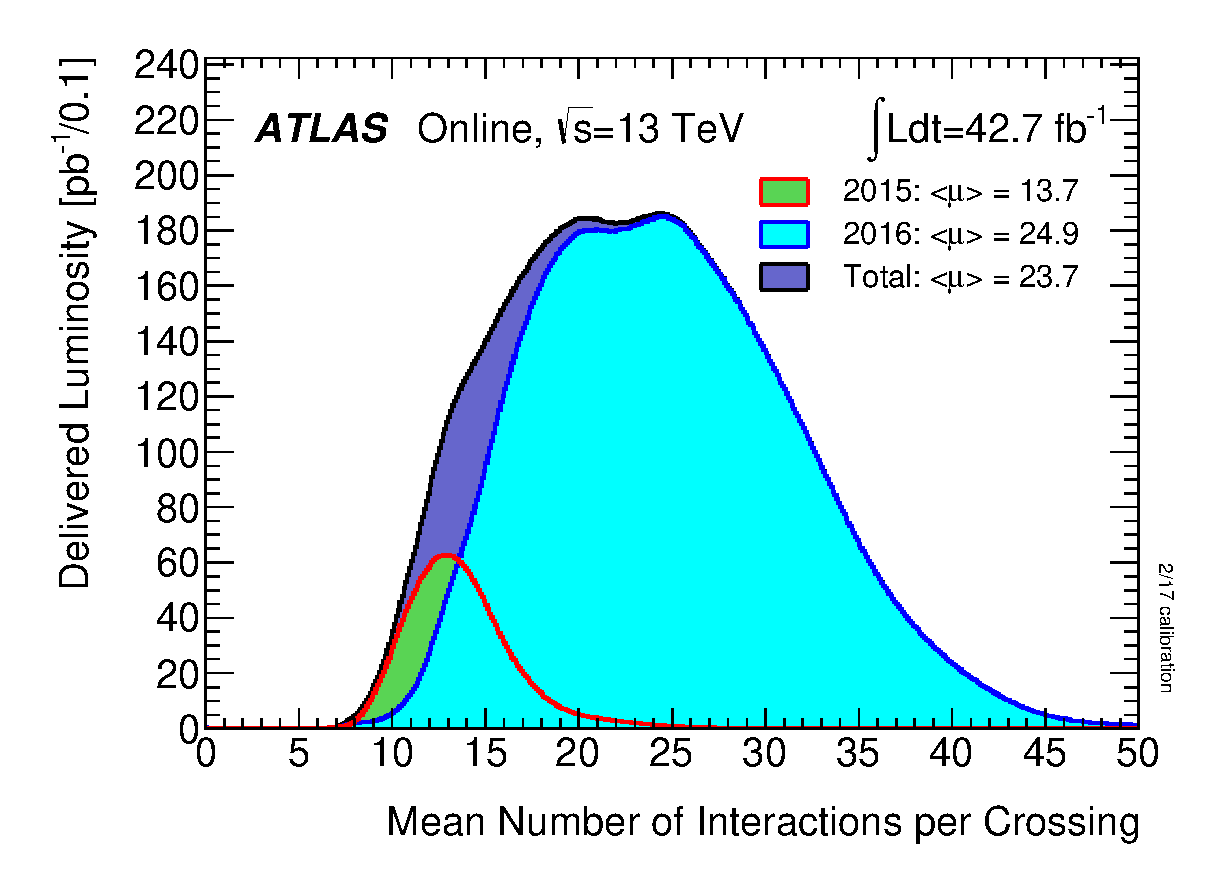
\includegraphics[width=0.53\textwidth]{figures/ATLAS/mu_2015_2016}
     \caption[ATLAS mean interactions per bunch crossing in 2016]{The luminosity weighted average number of interactions per bunch crossing, $\langle\mu\rangle$, for the 2015 and 2016 data taking periods~\cite{Lumi_Public_Run2}.}
     \label{fig:mu_2015_2016}
\end{wrapfigure}

The high luminosity environment at the LHC creates a dense background of overlapping tracks. ``Pileup'' (PU) events occur when there are simultaneous interactions during a bunch crossing, denoted by $\mu$ which reached an average value of 24.9 in 2016~\cite{Lumi_Public_Run2} (\Fig{\ref{fig:mu_2015_2016}}). Consistent and precise vertex identification is essential to mitigate pileup and maintain physics sensitivity. A Z boson candidate event with 25 reconstructed vertices is shown in~\Fig{\ref{fig:25_ver_zmumu}} to illustrate the importance of precise vertex reconstruction. 

The design and layout of the ID reflects a compromise of several competing requirements. The material budget in the tracking volume
%, shown in~\Fig{\ref{fig:id_mat_bud}}, 
should be minimized to reduce scattering and energy loss. However, 
%high rates require close proximity electronics, 
large particle flux requires radiation hardness, and high precision tracking requires a robust, rigid structure. High granularity near the IP must also be balanced with enough tracking volume to accurately measure the curvature of particles. The three layers of the ID attempt to address these design constraints: an innermost Pixel Detector, a Semiconductor Tracker (SCT), and a Transition Radiation Tracker (TRT).  
\begin{figure}[tbp]
    \begin{center}
    \includegraphics[width=0.8\textwidth]{figures/Atlas/25ver_zmumu}
    \caption[High vertex multiplicity event]{A candidate Z boson event decaying to two muons with 25 reconstructed vertices. This event was recorded on April 15th, 2012 and demonstrates the ATLAS high pileup environment~\cite{25_vertices_z}.}
    \label{fig:25_ver_zmumu}
    \end{center}
\end{figure}
%\begin{figure}[tbp]
%    \centering
%   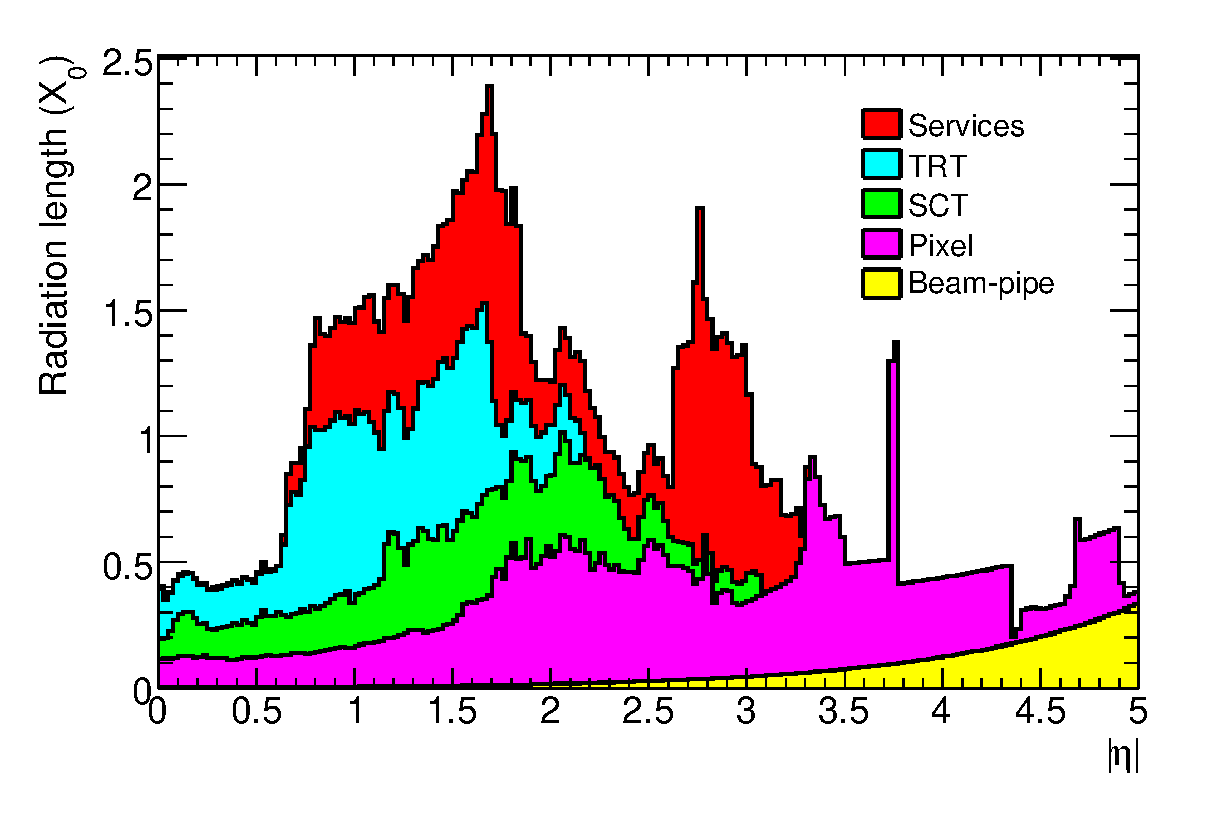
\includegraphics[width=0.58\textwidth]{figures/Atlas/id_mat_bud}
%  \caption[Inner Detector Material Budget]{Material distribution (in radiation lengths $X_0$) of the ID as a function of $|\eta|$, averaged over $\phi$~\cite{ATLAS}.}
% \label{fig:id_mat_bud}
%\end{figure} 


%
\subsection{Pixel Detector and Insertable B-Layer}
The primary objective of the Pixel Detector is to provide accurate impact parameter resolution, vertex identification, and short-lived particle identification for objects such as $b$-quarks and $\tau$-leptons.

The sensors~\cite{Pixel_Sensors} in the Pixel Detector are fabricated on silicon wafers using bipolar diodes on an n-type bulk. The readout side of the sensor uses n$^+$ doping\footnote{
	The\,$^{+}$ here denotes a relatively large amount of doping, near degenerate levels.
}, while the back side has an asymmetrically depleted p$^+$-n junction creating a reverse bias through the entire bulk. Particles passing through the bulk ionize it, allowing charge carriers to be collected on the sensor. A ``hit'' is registered if the amount of charge accumulated surpasses a threshold.

%Irradiation of the sensors eventually will lead to a type conversion of the bulk from n to p. Depletion begins on the p$^+$-n junction, lowering the effective doping until type conversion. Then, the junction will be on the readout (n) side isolating the pixels which allows operation below the depletion voltage.
%\footnote{The voltage required to fully deplete the bulk of charge carriers. Operating below this voltage is possible but brings about signal degradation.} 

The original Pixel Detector consists of three cylindrical layers,
%\footnote{The innermost layer, layer 0, is also sometimes called the B-layer or barrel layer. The two other layers are just known as layer 1 and layer 2.} 
concentric with the beam pipe, and three disk layers in the forward regions (both A and C side) perpendicular to the beam pipe. In 2014, a fourth innermost layer called the Insertable B-Layer (IBL) was installed, along with a new smaller radius beryllium beam pipe.
%\footnote{The radius was decreased from 29 mm to 25 mm.}
The spatial layout of the Pixel and IBL detectors is summarized in \Tab{\ref{tab:pixel_config}}. For clarity, descriptions of the Pixel Detector refer to the original three layers, whereas the IBL will be explicitly written to denote the new innermost layer.

The design and insertion of the IBL was meant to ready the ID for conditions up to the start of the High Luminosity LHC (HL-LHC), at which point ATLAS is projected to have recorded 300 fb$^{-1}$ of data. As modules in the innermost Pixel layer (B-layer) age, they may begin failing. Additionally, the peak luminosity will reach twice the design value of $10^{34}$ cm$^2$s$^{-1}$, leading to high PU\footnote{
	Projected $\langle\mu\rangle\sim 60$.
} and readout inefficiencies. The IBL serves to add robustness and redundancy to the tracking capabilities of the Pixel Detector. Improved performance at low $p_{\rm T}$ helps secure excellent tracking, impact parameter resolution, and $b$-tagging efficiency in a high PU environment~\cite{ID_RUN2_PROC}. 


\begin{table}[tbp]
\caption[Summary of ATLAS Pixel Detector configuration]{Spatial configuration and extent of the Pixel Detector and IBL system~\cite{IBL_TDR}.}
\label{tab:pixel_config}
\begin{center}
\begin{tabular}{lccccc}
	\hline
	\vbox{\hbox{\strut \textbf{Component}}\hbox{\strut}} & \vbox{\hbox{\strut \textbf{Radial}}\hbox{\strut  \textbf{Extension} [mm]}} & \vbox{\hbox{\strut \textbf{Length}}\hbox{\strut [mm]}} & \textbf{\vbox{\hbox{\strut Staves /}\hbox{\strut Sectors}}} & \vbox{\hbox{\strut \textbf{Modules}}\hbox{\strut }} & \vbox{\hbox{\strut \textbf{Pixels}}\hbox{\strut (x$10^6$)}}\\ \hline\hline
	Beam  Pipe & $25 < R < 29$ & & & & \\ \\
	\textbf{IBL} \\
	 & $\langle R\rangle = 33.25$ & $|Z| < 332$ & 14 & 224 & 12 \\ \\
	 \textbf{Pixel} \\
	 B-layer & $\langle R\rangle = 50.5$ & $|Z| < 400.5$  &22 & 286 & 13.2 \\
	 Layer 1 & $\langle R\rangle = 88.5$ & $ |Z| < 400.5$ & 38 & 494 & 22.8 \\
	 Layer 2 & $\langle R\rangle= 122.5$ & $|Z|< 400.5$  & 52 & 676 & 31.2 \\
	 Disk 1 & $88.8 < R < 149.6$ & $\langle Z\rangle = 495$ & $8\times2$ & $48\times2$ & 4.4 \\
	 Disk 2 & $88.8 < R < 149.6$ & $\langle Z\rangle = 580$ & $8\times2$ & $48\times2$ & 4.4 \\
	Disk 3 & $88.8 < R < 149.6$ & $\langle Z\rangle = 650$ & $8\times2$ & $48\times2$ & 4.4 \\
	&&&&\em{Pixel Total}& $80.4$\\
	\hline
\end{tabular}
\end{center}
\end{table}

%\begin{figure}[tbp]
%\begin{center}
%\includegraphics[width=.85\linewidth]{figures/ATLAS/ibl_layout_rev}
%\caption[IBL layout]{Layout of the IBL in the $R-\phi$ plane~\cite{IBL_TDR}.}
%\label{fig:ibl_layout}
%\end{center}
%\end{figure}

The IBL consists of approximately 12 million pixel channels. The main structure is comprised of 14 carbon-fibre cooling supports, called staves, set at a $14^{\circ}$ azimuthal tilt.
%\footnote{Measured as the tangent to the stave surface in the plane perpendicular to the cylinder axis.} (see \Fig{\ref{fig:ibl_layout}}) 
%The light carbon-fibre staves allow for a tiny 1.54\% $X_0$
%\footnote{Radiation length, average path in material for relativistic charged particle to lose 67\% of its energy.} 
%footprint. Each stave measures 2 cm (width) $\times$ 64 cm (length) and covers  a range in $\eta$ of approximately $\pm 3$. 
A stave holds 32 front-end chips (FE-I4) with 130 nm CMOS technology that are bump-bonded
%\footnote{Either electroplated solder (PbSn) or evaporative indium methods are used to attach the integrated circuit to the substrate. } 
to silicon sensors with 26,880 pixels each. 
%Each sensor has 80 columns $\times$ 336 rows of pixel cells (50 $\mu$m $\times$ 250 $\mu$m), for a total of 26,880 pixels per sensor. 
The central part of the stave utilizes $200 \mu$m thick planar n$^+$-in-n silicon sensors, while the forward ends of the stave carry new 3D n-in-p sensors with electrodes passing through the bulk. The $230\,\mu$m thick 3D sensors are more robust to irradiation with respect to the planar sensors. The transverse resolution of the IBL is $10\,\mu$m in $R-\phi$, while the longitudinal resolution is $75\,\mu$m in $z$.

Overall, the Pixel Detector has over 80 million pixel channels. In the cylindrical barrel region $|\eta|<2.5$, Pixel support staves are set at a $20^{\circ}$ azimuthal tilt.
% and a total material budget of 3\% $X_0$. 
%, the B-layer, layer 1, and layer 2 have 22, 38, and 52 cooling support staves respectively, each set at a $20^{\circ}$ azimuthal tilt. 
Each stave holds 13 modules with 16 front-end chips (FE-I3) with 250 nm CMOS technology that are bump bonded to silicon sensors with 46,080 pixels each. 
%The 250\,$\mu$m thick planar n$^+$-in-n sensors feature 18 columns $\times$ 160 rows of pixel cells ($50 \mu$m $\times$ $400 \mu$m), for a total of 46,080 pixels per sensor. 
The three disks on each end-cap cover $2.0< |\eta| < 2.5$ and are split into 8 sectors
\footnote{A sector is the end-cap analogue of staves in the barrel region.} 
with 6 sensors each (identical to those in the barrel). The Pixel Detector has a transverse resolution of $10\,\mu$m in $R-\phi$, and a longitudinal resolution of $115\,\mu$m in $z$ ($R$) in the barrel (end-cap) region. 

%
\subsection{Semiconductor Tracker}

The Semiconductor Tracker (SCT) provides on average four precise position measurements per track at intermediate radial distances in order to guarantee excellent track reconstruction and charged particle \pt resolution.

Sitting at a farther distance from the IP, the SCT~\cite{SCT_paper} has relaxed radiation hardness and spatial resolution requirements. In contrast with the Pixel Detector, therefore, the SCT uses AC-coupled single-sided silicon micro-strips with p$^+$ strip implants in an n-type bulk to control for costs and reliability with over 63 m$^2$ of silicon. 

\begin{figure}[tbp]
\begin{center}
\includegraphics[width=.9\linewidth]{figures/ATLAS/SCT_Quadrant}
\caption[Semiconductor Tracker layout]{Layout of the SCT in the $R-z$ plane~\cite{SCT_paper}.}
\label{fig:sct_layout}
\end{center}
\end{figure}

The layout of the SCT, shown in \Fig{\ref{fig:sct_layout}}, is similar to that of the Pixel Detector: there are four concentric barrel layers
%\footnote{The numbering scheme is B3, B4, B5, B6.} 
positioned between radii $R_3=299$\,mm and $R_6=514$\,mm, and nine forward disks with up to three rings on either end-cap situated between $z_1=853.8$\,mm and $z_9=2720.2$\,mm. Over 6.3 million channels, covering $|\eta|<2.5$, are spread over 4088 modules that tile the SCT: 2112 rectangular modules in the barrel at an $11^{\circ}$ tilt, and 1976 trapezoidal modules in the disks. Most modules feature two 285\,$\mu$m thick sensors back-to-back with a stereo angle of 40 mrad. A layer will thus register two strip measurements, which are combined to obtain the $z$ position and create a space-point. Each sensor has 768 strips with a pitch of 80\,$\mu$m
\footnote{The wedge modules in the disks have varying pitches between $50-90\,\mu$m.} 
and length of 63\,mm. Two sensors on each side of the module are daisy-chained to create a total strip length of 126\,mm.  The SCT has a transverse resolution of $17\,\mu$m in $R-\phi$, and a longitudinal resolution of $580\,\mu$m in $z$ (R) in the barrel (end-cap) region.



%
%\clearpage
\subsection{Transition Radiation Tracker}
The Transition Radiation Tracker (TRT) provides continuous tracking for particles within $|\eta|<2$, by registering on average 36 hits per track. Additionally, the TRT is capable of particle identification by differentiating between electrons and hadrons by using transition radiation.

The TRT is comprised of approximately 300,000 gas-filled polyimide drift tubes~\cite{TRT_sensors}, called straw tubes, of diameter 4\,mm. In the barrel, 52,544 straws with a length of 144\,cm are positioned parallel to the beam axis  and cover $|\eta| < 1$. Each end-cap features 122,880 straws aligned radially on two types of wheels with a length of 37\,cm covering $1<|\eta|<2$. The spatial extent of the TRT is shown in \Tab{\ref{tab:trt_layout}}.

\begin{table}[tbp]
\begin{center}
\caption[Transition Radiation Tracker spatial layout]{Layout of the barrel and end-cap modules of the TRT.}
\label{tab:trt_layout}
\begin{tabular}{llllll}
\hline
\textbf{Component} & $|z_{\text{min}}|$ [mm]& $|z_{\text{max}}|$ [mm]& $|R_{\text{min}}|$ [mm]& $|R_{\text{max}}|$ [mm] & \textbf{Straws} \\ \hline\hline
TRT barrel & 0 & 712 & 563 & 1,066 & 52,544\\
TRT end-cap & 848 & 2710 & 644 & 1,004 & 122,880 \\ 
\hline
\end{tabular}
\end{center}
\end{table}

%\begin{figure}[htbp]
\begin{wrapfigure}{r}{.55\textwidth}
\begin{center}
	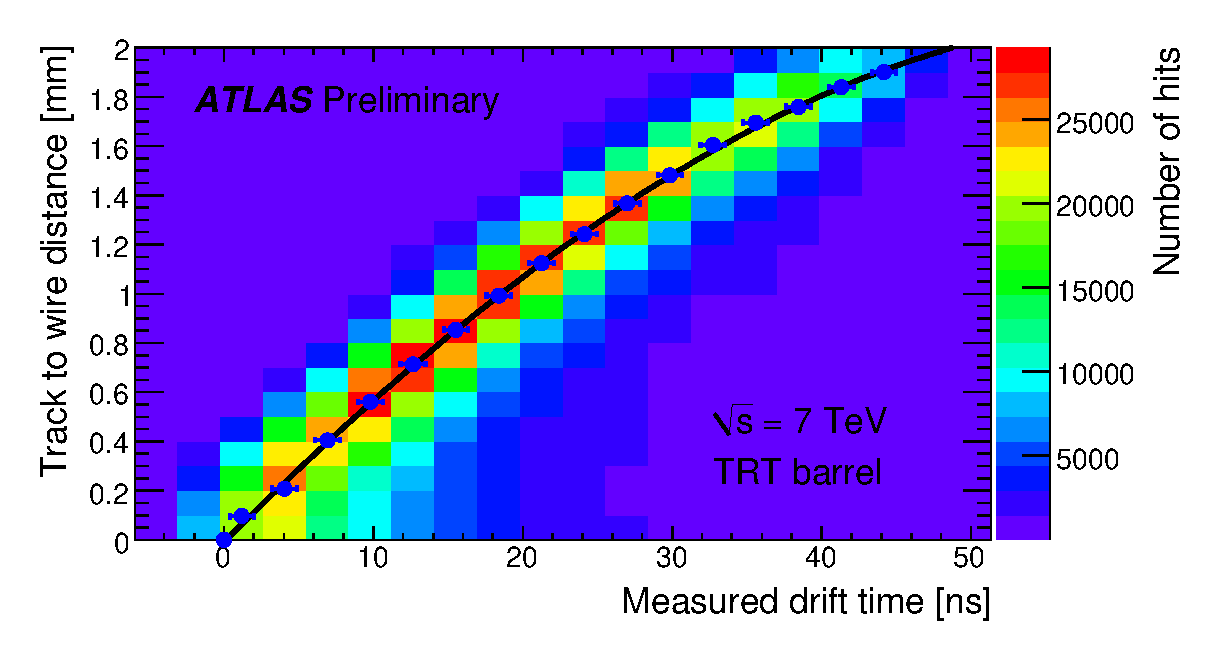
\includegraphics[width=.99\linewidth]{figures/ATLAS/trt_drift}
	\caption[Transition Radiation Tracker wire impact parameter vs drift time]{Using the drift time, the distance from the track to the wire can be inferred. The dependency of the drift radius on measured drift time can be fit with a third order polynomial~\cite{trt_twiki}.}
	\label{fig:trt_drift}
\end{center}
\end{wrapfigure}
%\end{figure}

The walls of the straw tubes are made with two bonded 35\,$\mu$m film layers
%\footnote{The film consists of a 25\,$\mu$m thick Kapton film, coated with a 0.2\,$\mu$m Al-deposit and 5-6\,$\mu$m thick graphite-polyimide layer. The other side is coated with 4-5\,$\mu$m thick polyurethane sealant layer.} 
reinforced with carbon fibres. Through the center of each straw tube is a grounded 31\,$\mu$m diameter gold-plated
%\footnote{Approximately 0.5-0.7\,$\mu$m thick.} 
tungsten wire which functions as an anode. The walls of the straws are kept at a -1.53\,kV potential and act as the cathode. The straws are filled with a gaseous mixture of 70\% Xe, 27\% CO$_2$, and 3\% O$_2$.
%\footnote{In Run-2, Ar replaced Xe in straws with gas leaks. Ar provides similar tracking performance; however, it detects transition radiation more poorly than Xe in the operational energy range.}
The volume between each straw is filled with polymer fibres (foils) in the barrel (end-cap) region to create transition radiation.

As charged particles pass through the TRT, the gas in the straws is ionized. The free electrons drift along the lines of the applied potential and are collected on the anode, where the readout signal is compared to a threshold.  By measuring the drift time of particles in the TRT, the distance to the wire from the particle, or drift distance, can be inferred, as depicted in~\Fig{\ref{fig:trt_drift}}. The drift time measurement provides an inherent transverse ($R-\phi$) spatial resolution of 130\,$\mu$m per straw.

Low energy transition radiation is emitted by relativistic charged particles as they traverse a boundary in which the two mediums exhibit different dielectric permittivities. The space filling polymer fibres and foils allow for such radiation to be produced in the TRT. The transition radiation photons are absorbed by the Xe gas in the straws producing a stronger signal response. The amount of transition radiation detected can be used to differentiate
%\footnote{The amount of radiation is proportional to the relativistic factor, $\gamma=E/m$. Electrons will thus have a much stronger response than hadrons.} 
electrons from hadrons, through the use of a second higher readout threshold. 


%%
\section{Calorimetry}

The ATLAS calorimeters~\cite{LAr_TDR,Tile_TDR}, shown in~\Fig{\ref{fig:cal_layout}}, surround the ID and solenoid magnet and aim to fully absorb and provide precise measurements of electrons, photons, jets, and \MET over the range $|\eta|<4.9$. The Liquid Argon (LAr) and Tile Calorimeters are sampling calorimeters: dense layers (absorbers) which induce particle showers alternate with active layers which measure the deposited energy\footnote{
	Since some energy is deposited in the absorbers, the total energy must be estimated from the ``sampled" shower energy in the active layers.
}.

\begin{figure}[tbp]
\begin{center}
\includegraphics[width=0.8\textwidth]{figures/ATLAS/calorimeter_layout}
\caption[Layout of Liquid Argon and Tile calorimters]{Diagram of the Liquid Argon and Tile Calorimeters which sit outside the Inner Detector and solenoid magnet~\cite{ATLAS}.}
\label{fig:cal_layout}
\end{center}
\end{figure}

The particle showers produced from electromagnetic (EM) particles and those produced from hadronic particles behave differently; thus, two types of calorimeters (EM and hadronic) are designed to cater to each  shower type. LAr EM calorimeters cover $|\eta|<3.2$, LAr hadronic calorimeters cover $1.5<|\eta|<4.9$, and Tile hadronic calorimeters cover $|\eta|<1.7$. Since hadronic showers penetrate deeper than EM showers, the EM calorimeters are placed before the hadronic calorimeters. To characterize the thickness of a material as seen by the EM radiation, the radiation length, $X_0$, measures both the average distance required to lower high energy electrons to $1/e$ its initial energy via Bremsstrahlung, and also $7/9$ the mean free path for high energy photons to undergo pair production. The nuclear interaction length, $\lambda$, measures the average distance traveled by a hadron before interacting with a nucleus.

Each type of calorimeter optimizes separately the choice of material and thickness for the absorber and active layers, as well as the cell size. If particle showers are not fully contained in the calorimeters, some shower particles may penetrate the surrounding Muon Spectrometer, known as ``punch-through''. To prevent punch-through\footnote{
	The goal is two-fold: (1) calorimeter objects which reach the muon spectrometer can induce fake muon rates, and (2) an accurate \MET measurement requires containment of the full EM and hadronic showers.
}, the total thickness of the EM calorimeters, shown in~\Fig{\ref{fig:x0_cal}}, is approximately $22\,X_0$ in the barrel and $24\,X_0$ in the end-cap region, while the total thickness of the hadronic calorimeters, shown in~\Fig{\ref{fig:lambda_cal}}, is approximately $10\,\lambda$. 

\begin{figure}[htbp]
\begin{center}
\subfloat[]{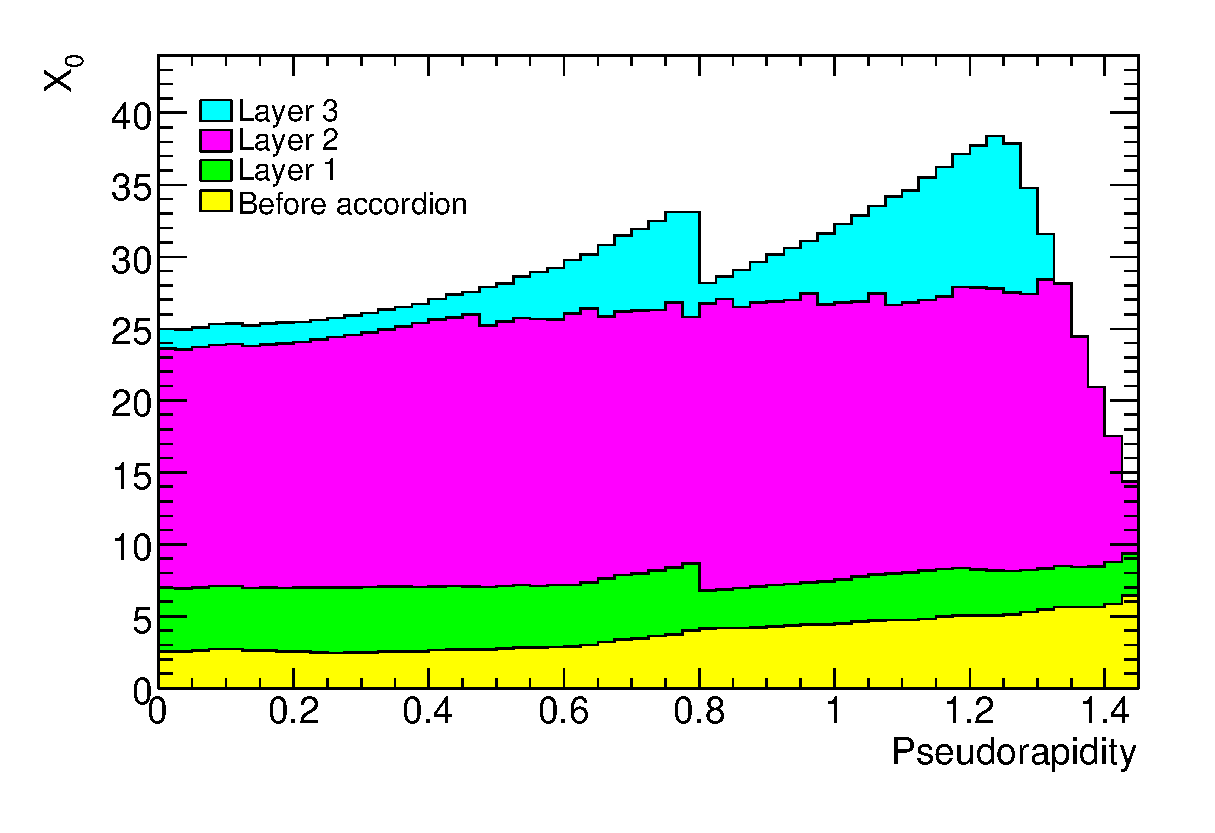
\includegraphics[width=0.49\textwidth]{figures/ATLAS/x0_barrel}\label{fig:x0_cala}}
\subfloat[]{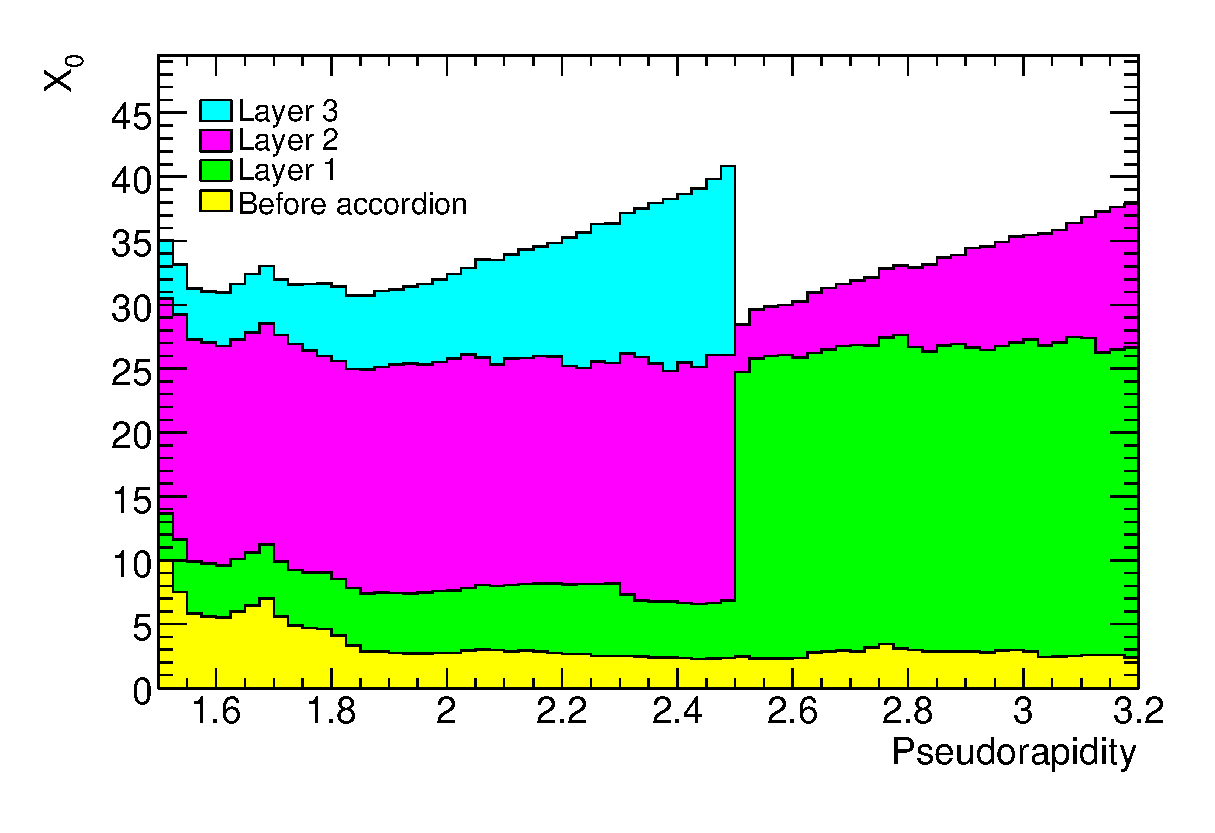
\includegraphics[width=0.49\textwidth]{figures/ATLAS/x0_endcap}\label{fig:x0_calb}}
\caption[Radiation lengths in ATLAS electromagnetic calorimeters]{Total thickness in radiation lengths, $X_0$, of the EM calorimeters in \protect\subref{fig:x0_cala} the barrel and \protect\subref{fig:x0_calb} the end-cap region~\cite{ATLAS}.}
\label{fig:x0_cal}
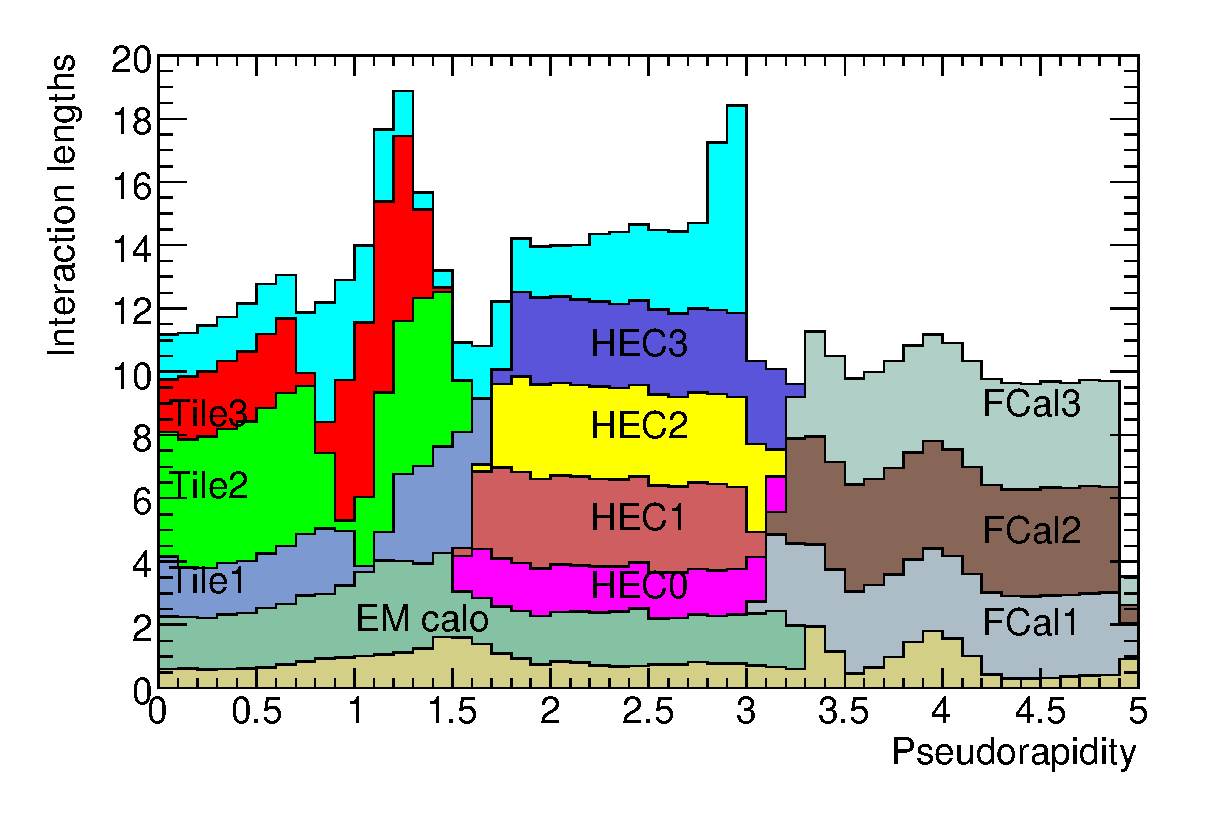
\includegraphics[width=0.8\textwidth]{figures/ATLAS/lambda_cal}
\caption[Interaction lengths in ATLAS calorimeters]{Total thickness in nuclear interaction lengths, $\lambda$, of the ATLAS calorimeters~\cite{ATLAS}.}
\label{fig:lambda_cal}
\end{center}
\end{figure}

%
\subsection{Particle Showers}
\label{ch:atlas:particle_showers}
The calorimeters measure energy of an incoming particle by sampling the energy of the induced particle showers. EM and hadronic showers involve different physics processes and therefore develop differently in the detector\cite{pdg_2017}. 

Electrons, positrons and photons produce EM showers: energetic electrons radiate Bremsstrahlung photons, while energetic photons convert to electron-positron pairs when traversing dense material. The longitudinal depth of an EM shower is expressed in terms of the radiation length and critical energy, $E_c$\footnote{
	The critical energy $E_c\propto \frac{1}{Z}$ measures the energy at which energy loss from ionization (logarithmic with energy) is comparable to energy lost from Bremstrahlung (linear with energy), above which Bremstrahlung dominates. The radiation length $X_0\propto Z(Z+1)$ \cite{pdg_2017}. 
}, in \Eqn{\ref{eq:x0}}.
\begin{equation}
	X = X_0\frac{\ln\left(E_0/E_c\right)}{\ln 2}
	\label{eq:x0}
\end{equation}

Hadronic showers involve distinct processes to those of EM showers, including hadron production from QCD radiation, pion decays, and de-exciting nuclei. Approximately half of the energy of the hadron is transferred to secondary hadrons produced in the shower. About one third of the energy dissipated in the hadronic shower is via neutral pions which decay via $\pi^0\to\gamma\gamma$ and produce an EM component of the shower. Additionally, particles may interact with the nuclei in the absorber in a variety of nuclear processes, which then produce additional particles near the MeV scale.  The longitudinal depth of the hadronic shower scales with the nuclear interaction length, $\lambda\propto A^{\frac{1}{3}}$. 


%
\subsection{Liquid Argon Calorimeter}

With over 180,000 channels, the LAr calorimeters consist of both EM and hadronic modules. The LAr EM calorimeters are divided into the barrel (EMB) region covering $|\eta|<1.475$ and two coaxial end-cap regions (EMEC) covering $1.375<|\eta|<3.2$. The EMB consists of two cylindrical half-barrels, each 3.2\,m in length with an inner (outer) diameter of $2.8$\,m ($4$\,m). The wheels of the EMEC are 63\,cm thick and extend radially between $R=330$\,mm and $R=2098$\,mm.  Each end-cap wheel is divided into an inner wheel from $1.375<|\eta|<1.5$ and an outer wheel from $1.5<|\eta|<3.2$. Accordion-shaped lead absorber plates alternate with similarly shaped copper-kapton electrodes, with liquid argon filling the bulk as the active medium. The accordion structure ensures complete $\phi$ coverage with no gaps. In the barrel the accordion folds are axial while in the end-cap they are radial. The angle and amplitude of the folds varies with radius to ensure constant gaps.

Incident particles shower in the absorber layer, and ionize the LAr. The electrodes are kept near $2$\,kV to allow the electrons to drift through 2.1\,mm gaps on either side of the electrodes, which corresponds to a relatively slow drift time of $450$\,ns. The electrodes collect a triangular pulse which is then shaped and sampled once every 25\,ns, as shown in~\Fig{\ref{fig:lar_pulse}}. In Run I (Run II), five (four) samples of the shaped pulse were read out to reconstruct the time and energy of the pulse. As the pulse spans multiple bunch crossings, care must be taken to account for out-of-time PU due to collisions in nearby bunches.

%\begin{figure}[tbp]
\begin{wrapfigure}{r}{0.52\textwidth}
\begin{center}
\includegraphics[width=0.5\textwidth]{figures/ATLAS/lar_pulse}
\caption[Liquid Argon calorimeter signal pulse]{The triangular pulse shape response from the LAr calorimeter, overlaid with the pulse after shaping and sampling.~\cite{ATLAS}.}
\label{fig:lar_pulse}
\end{center}
\end{wrapfigure}
%\end{figure}

In the region $|\eta|<2.5$, the EM calorimeters are segmented into three depth layers as shown in~\Fig{\ref{fig:lar_cross}}. The first ``strip'' layer provides precise $\eta$ measurements with a granularity of $\Delta\eta\times\Delta\phi=0.0031\times0.02545$. The fine $\eta$ segmentation helps differentiate photons from neutral pions decaying to two photons, and provides precise flight direction for neutral particles. The second layer has a coarser resolution of $\Delta\eta\times\Delta\phi=0.025\times0.0245$. However, it has a larger depth in order to absorb the bulk of the EM radiation in the showers. The final layer principally measures the remaining energy from the most energetic particles, while attempting to distinguish EM from hadronic objects. 

As the EM calorimeters sit outside the solenoid magnet, shower development has already begun by the time particles reach them. A separate, 11\,mm-thin pre-sampler layer of liquid argon sits in front of the solenoid magnet, and covers $|\eta|<1.8$. This permits earlier sampling of showers and provides a measurement of the energy lost in front of the calorimeter. 

The hadronic end-cap (HEC) also uses LAr as an active medium. However, it uses parallel copper plate absorbers instead of lead. Covering $1.5<|\eta|<3.2$, each HEC end-cap consists of two wheels with 32 identical wedge-shaped modules. The front (back) wheels have 24 (16) copper plates, each 25 (50)\,mm thick. The plates are kept with an 8.5\,mm gap between them, through which three electrodes create four drift zones. The front wheel has a granularity of $\Delta\eta\times\Delta\phi=0.1\times0.1$ while the back wheel has four times coarser granularity.

\begin{figure}[tb]
\begin{center}
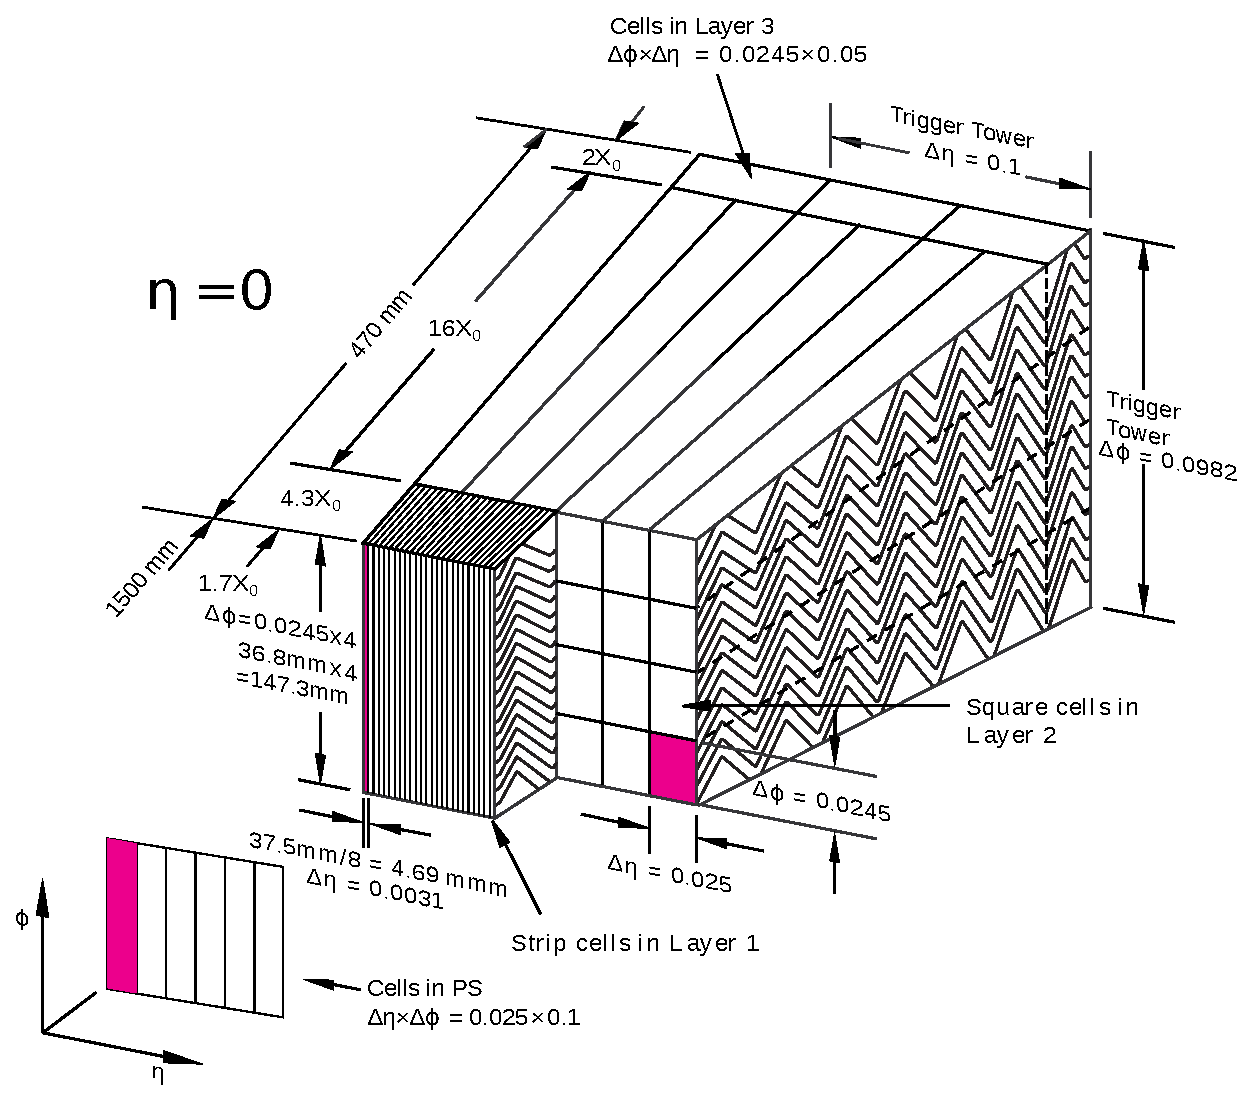
\includegraphics[width=0.8\textwidth]{figures/ATLAS/lar_cross}
\caption[Liquid Argon electromagnetic calorimeter layout]{Sketch of the accordion structure of the EM calorimeter showing the layers and granularity in $|\eta|$ and $\phi$~\cite{LAr_TDR}.}
\label{fig:lar_cross}
\end{center}
\end{figure}

%\begin{figure}[tbp]
%\begin{wrapfigure}{r}{0.52\textwidth}
%\begin{center}
%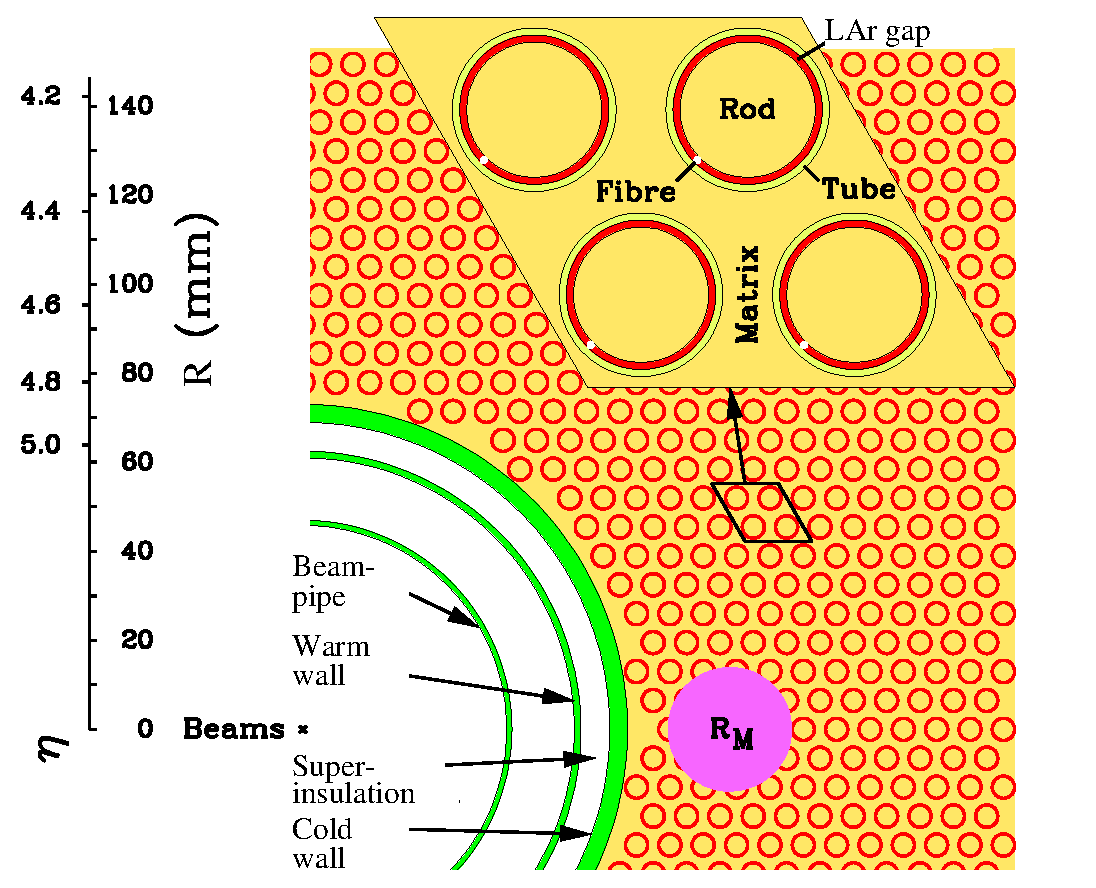
\includegraphics[width=0.5\textwidth]{figures/ATLAS/fcal_layout}
%\caption[LAr FCal structure]{FCal1 layout showing the LAr gap between the copper tubes and rods~\cite{ATLAS}.}
%\label{fig:fcal_layout}
%\end{center}
%\end{wrapfigure}
%\end{figure}

Sitting inside the HEC, the forward calorimeter (FCal) provides coverage from $3.1<|\eta|<4.9$. Due to its proximity to the beam pipe, the FCal experiences extremely large particle fluxes. To combat ion build-up, the LAr gap sizes are much smaller. Three 45\,cm deep modules make up the FCal: the first module (FCal1) is electromagnetic, while the two modules at larger $|z|$ (FCal2, FCal3) are hadronic. 
%Depicted in~\Fig{\ref{fig:fcal_layout}}, 
FCal1 consists of copper plates with holes drilled for cylindrical electrodes to pass through, parallel to the beam pipe. The electrodes consist of a copper rod inside a copper tube with a 269\,$\mu$m gap. Copper was chosen for FCal1 in order to quickly dissipate heat, while tungsten was chosen for the hadronic FCal2 and FCal3 modules in order to maximize containment of the hadronic showers. The FCal2 (FCal3) electrodes consist of a tungsten rod inside a copper tube with a 375 (500)\,$\mu$m gap and are surrounded by tungsten slugs. 

%
\subsection{Tile Calorimeter}

Sitting outside the LAr calorimeters in the barrel region is the hadronic Tile calorimeter. A 5.8\,m long main barrel covers $|\eta|<1.0$ and two 2.8\,m long extended barrels (EB) cover $0.8<|\eta|<1.7$. The cylindrical Tile calorimeter barrels extend radially from $R=2.28$\,m to $R=4.25$\,m, and are segmented into three depth layers. The hadronic Tile calorimeter is a sampling calorimeter consisting of steel absorber plates and scintillating plastic tiles serving as the active medium.

%\begin{figure}[htbp]
\begin{wrapfigure}{r}{0.52\textwidth}
\begin{center}
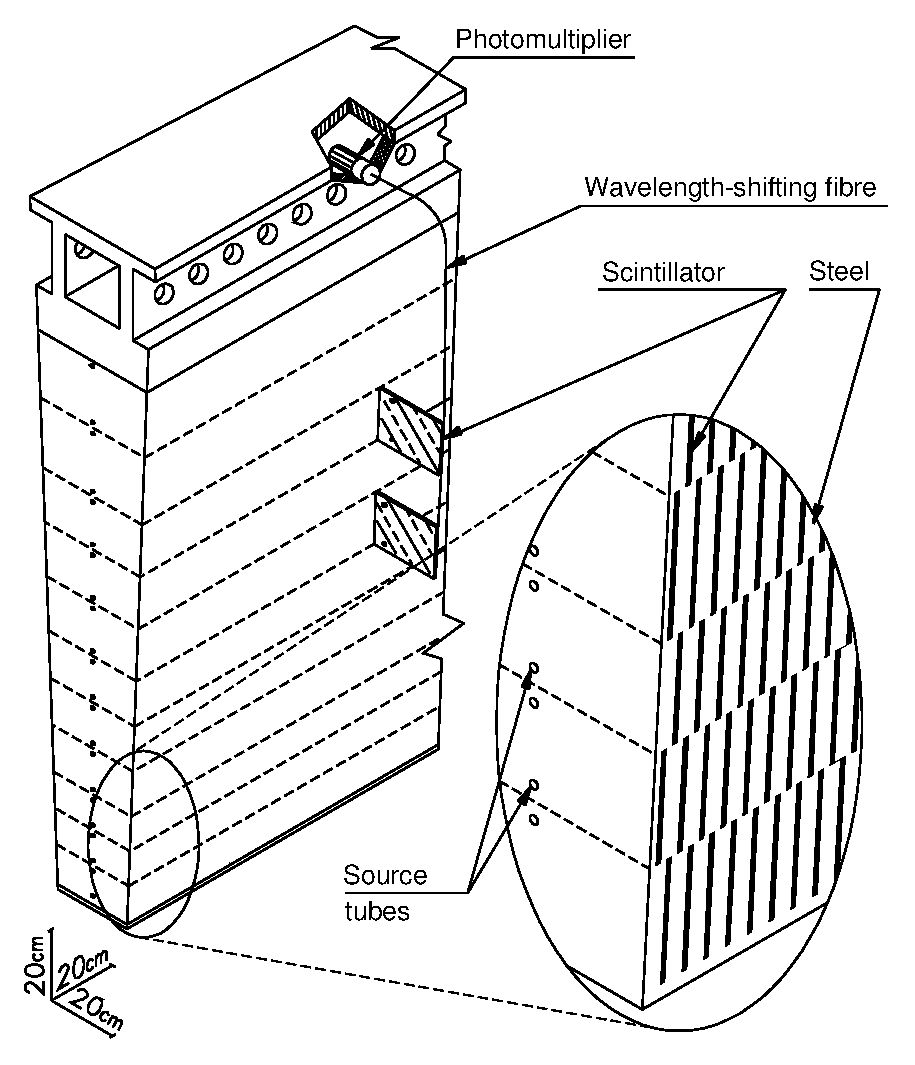
\includegraphics[width=0.5\textwidth]{figures/ATLAS/TileCal_Module}
\caption[Tile calorimeter module]{Layout of a wedge-shaped module in the Tile calorimeter with alternating steel absorber plates and plastic scintillating tiles~\cite{ATLAS}.}
\label{fig:tilecal}
\end{center}
\end{wrapfigure}
%\end{figure}


High energy particles striking the tile scintillators produce ultraviolet ``scintillation'' light, which is collected in wavelength-shifting fibres at either end of the tile. These fibres lengthen the wavelength of the ultraviolet scintillation to the visible spectrum and are fed into photomultiplier tubes. Groups of fibres are used to define read-out cells and three depth layers: cells in the two innermost depth layer have a granularity of $\Delta\eta\times\Delta\phi=0.1\times0.1$ while cells in the outermost layer have a granularity of $\Delta\eta\times\Delta\phi=0.2\times0.1$.

The main barrel and two EBs consist of 64 wedge-shaped modules that span $\Delta\phi=0.1$, as shown in~\Fig{\ref{fig:tilecal}}.  The plastic scintillator tiles are 3mm thick and vary in size depending on the radial position. In terms of interaction length, the thickness of the three depth layers of the main barrel (EB) are $1.5\lambda$, $4.1\lambda$, and $1.8\lambda$ ($1.5\lambda$, $2.6\lambda$, and $3.3\lambda$) from innermost to outermost. 

%%
\section{Muon Spectrometer}
As muons pass through the calorimeters, they lose much less energy than electrons to Bremsstrahlung radiation,
%\footnote{The total power radiated is inversely proportional to powers of the particle's mass.} 
and as a result, they are not contained in the calorimeters.
%\footnote{Also significant is that the muon lifetime is long enough to reach outside the calorimeters, as opposed to the heavy tau particles which decay in the ID.} 
Since muon tracks in the ID can suffer from poor momentum resolution at high \pt,
%\footnote{For very large \pt, tracks will have almost no curvature; thus, the accuracy of the momentum measurement will suffer.}
and relatively little muon energy is deposited in the calorimeters, a precision muon tracker~\cite{Muon_TDR} is placed outside the calorimeters to precisely measure muon momentum and position in the $R-z$ plane for $|\eta|<2.7$.  Additionally, muon triggering chambers are included to provide accurate bunch crossing identification and quick triggering decisions for $|\eta|<2.4$. The muon system is depicted in~\Fig{\ref{fig:mu_layout}}.  A summary of the coverage, resolution, and average number of hits for each component of the muon system is presented in~\Tab{\ref{tab:muon_cov}}.

\begin{figure}[htbp]
\begin{center}
\includegraphics[width=0.8\textwidth]{figures/ATLAS/muon_layout}
\caption[Layout of Muon Spectrometer]{Diagram of the Muon Spectrometer~\cite{ATLAS}.}
\label{fig:mu_layout}
\end{center}
\end{figure}

\begin{table}[htbp]
\begin{center}
\begin{tabular}{lr|llll|ll}
\hline
%\vbox{\hbox{\strut \textbf{Component}}\hbox{\strut}}
\textbf{Sub-} &\textbf{Coverage} &\multicolumn{3}{r}{\textbf{Resolution}}&& \textbf{Avg.}&  \textbf{Type}\\
\textbf{detector}& & $z$ & $R$ & $\phi$ [mm] & $t$ [ns]& \textbf{Hits}&\\\hline\hline
MDT & $|\eta|<2.7$          & $35\,\mu$m & --- & --- &---& 20 & Precision \\
CSC & $2.0<|\eta|<2.7$   & --- & $40\,\mu$m & 5 & 7 & 4 & Precision \\
RPC & $|\eta|<1.1$        & $10$\,mm & --- & 10 & 1.5 & 6 & Trigger \\
TGC & $1.1<|\eta|<2.4$ & --- & 2-6 mm & 3-7 & 4 & 9 & Trigger \\
\hline
\end{tabular}
\caption[Coverage and performance of the muon system]{Summary of coverage, resolution, and function of each component of the Muon System.}
\label{tab:muon_cov}
\end{center}
\end{table}

%
\subsection{Precision Chambers}
In the barrel region, three layers of precision tracking Monitored Drift Tube (MDT) chambers in cylindrical shells are located on and between the eight toroidal barrel magnets, approximately at radii of $5$\,m, $7.5$\,m, and $10$\,m. In the end-cap region, wheels (with three layers) sit in front of and behind the end-cap toroidal magnets, approximately at $|z| =$ 7.4\,m, 10.8\,m, 14\,m, and 21.5\,m. The MDT is made out of pressurized 30\,mm diameter drift tubes filled with 93\,\% Ar and 7\,\% CO$_2$ gas at 3 bar. As passing muons ionize the gas, the electrons are collected on a centered, 50\,$\mu$m diameter tungsten-rhenium wire at a potential of 3080\,V. An MDT chamber consists of tubes grouped into three to eight layers where the tube (chamber) has a resolution in $z$ of 80 (35)\,$\mu$m. In order to try to avoid coverage gaps, 1,150 MDT chambers housing over 354,000 channels are arranged so that adjacent chambers overlap in $\phi$.

The Ar/CO$_2$ gas mixture has a relatively long drift time, reaching up to 700\,ns. This requires a large dead time
%\footnote{An interval in which the tube is no longer allowed to register a hit.} 
and leaves the tube susceptible to deteriorating resolution at high occupancies.
%\footnote{The slow drift time combined with high occupancies leads to ion build-up and a distortion of the electric field.}
The tubes will be expected to register hits up to 30\,kHz at nominal LHC operation due to backgrounds, including conversions of photons and neutrons.

To address the issues of high occupancy faced by the MDT in the forward region, Cathode Strip Chambers (CSC) are used on the innermost tracking layer for $2.0<|\eta|<2.7$. The CSC are multi-wire proportional chambers where the cathodes are segmented into strips, filled with an Ar (80\,\%) and CO$_2$ (20\,\%) mixture. The series of radial anode wires are separated by 2.5\,mm and sit between cathode sheets divided into 1.6\,mm strips. One layer of cathode strips is perpendicular to the anode wires, providing the precision coordinate with a resolution in $R$ of 60\,$\mu$m. The other layer is parallel to the anode wire, providing the transverse coordinate with a resolution in $\phi$ of 5\,mm. Charge collected on neighboring cathode strips is interpolated to derive a position measurement. In total, there are 32 CSC chambers with 31,000 channels.

The CSC chamber configuration allows for a much smaller drift time of 40\,ns, yielding a time resolution of 7\,ns.  While safe operation of the MDT can be reached with muon flux up to 150\,Hz/cm$^2$, the CSC can operate safely up to 1000\,Hz/cm$^2$. The chamber schematics of the MDT and CSC are shown in~\Fig{\ref{fig:muon_tracking}}.


\begin{figure}[htbp]
\begin{center}
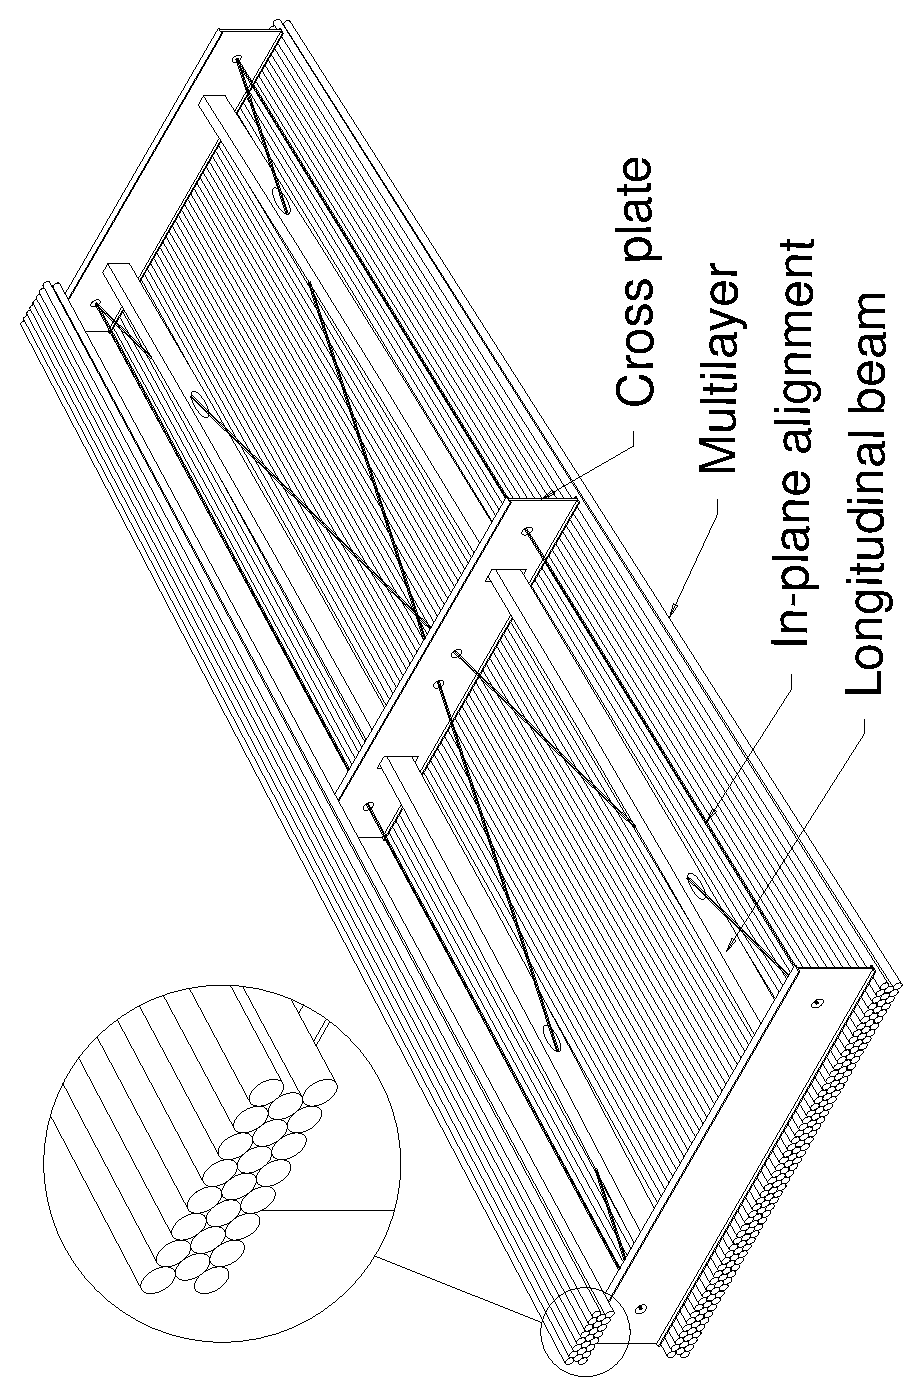
\includegraphics[angle=-90,origin=c,width=0.4\textwidth]{figures/Atlas/MDTchamber}
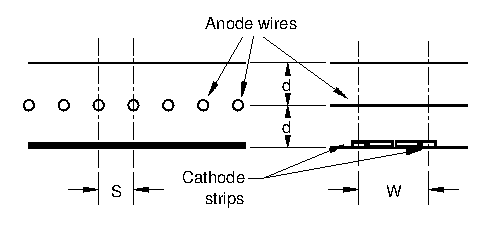
\includegraphics[width=0.59\textwidth]{figures/Atlas/CSC}
\end{center}
\caption[Schematic of muon precision tracking chambers]{A schematic of the MDT (left) and CSC (right) muon precision tracking chambers is shown~\cite{Muon_TDR}.}
\label{fig:muon_tracking}
\end{figure}

%
\subsection{Trigger Chambers}
In addition to the precision tracking capabilities provided by the MDT and CSC, the MS includes two triggering chambers, shown in~\Fig{\ref{fig:muon_trigger}}. 606 Resistive Plate Chambers (RPC) operate in the barrel region for $|\eta|<1.05$, while 3,588 Thin Gap Chambers (TGC) operate in the end-cap region for $1.05<|\eta|<2.4$. Due to the slow drift time of the MDT, assigning events to a specific bunch crossing requires additional input. The RPC and TGC were therefore designed to have sufficiently precise temporal resolution to assign muons to specific bunch crossings, making it possible to make event-by-event triggering decisions for specified \pt thresholds. Additionally, the coordinate of tracks perpendicular to the bending plane is provided by the triggering chambers.

The barrel RPC contain no wires: two resistive, parallel plates made of phenolic-melaminic plastic laminate are separated by 2\,mm with insulating spacers, while a gaseous mixture of 94.7\,\% C$_2$H$_2$F$_4$, 5\,\% Iso-C$_4$H$_{10}$, and 0.3\,\% SF$_6$ fills the interior. An electric field of 4.9\,kV/mm is applied between the plates, which facilitates avalanches
%\footnote{This is distinct from most other gas detectors in ATLAS which operate in proportional mode rather than avalanche mode.} 
from passing muons ionizing the gas. A thin layer of graphite is painted on the outside of the resistive plates, forming the HV and ground electrodes. Signals are read out via capacitively coupled pick up strips: 17\,$\mu$m thick copper strips are placed on the outside of the plates
%\footnote{The direction of the strips is perpendicular between the two plates.} 
with insulating 190\,$\mu$m PET film. Besides having a low operational voltage, the selected gas for the RPC has a low drift time, enabling a time resolution of 1.5\,ns. 

\begin{figure}[tb]
\begin{center}
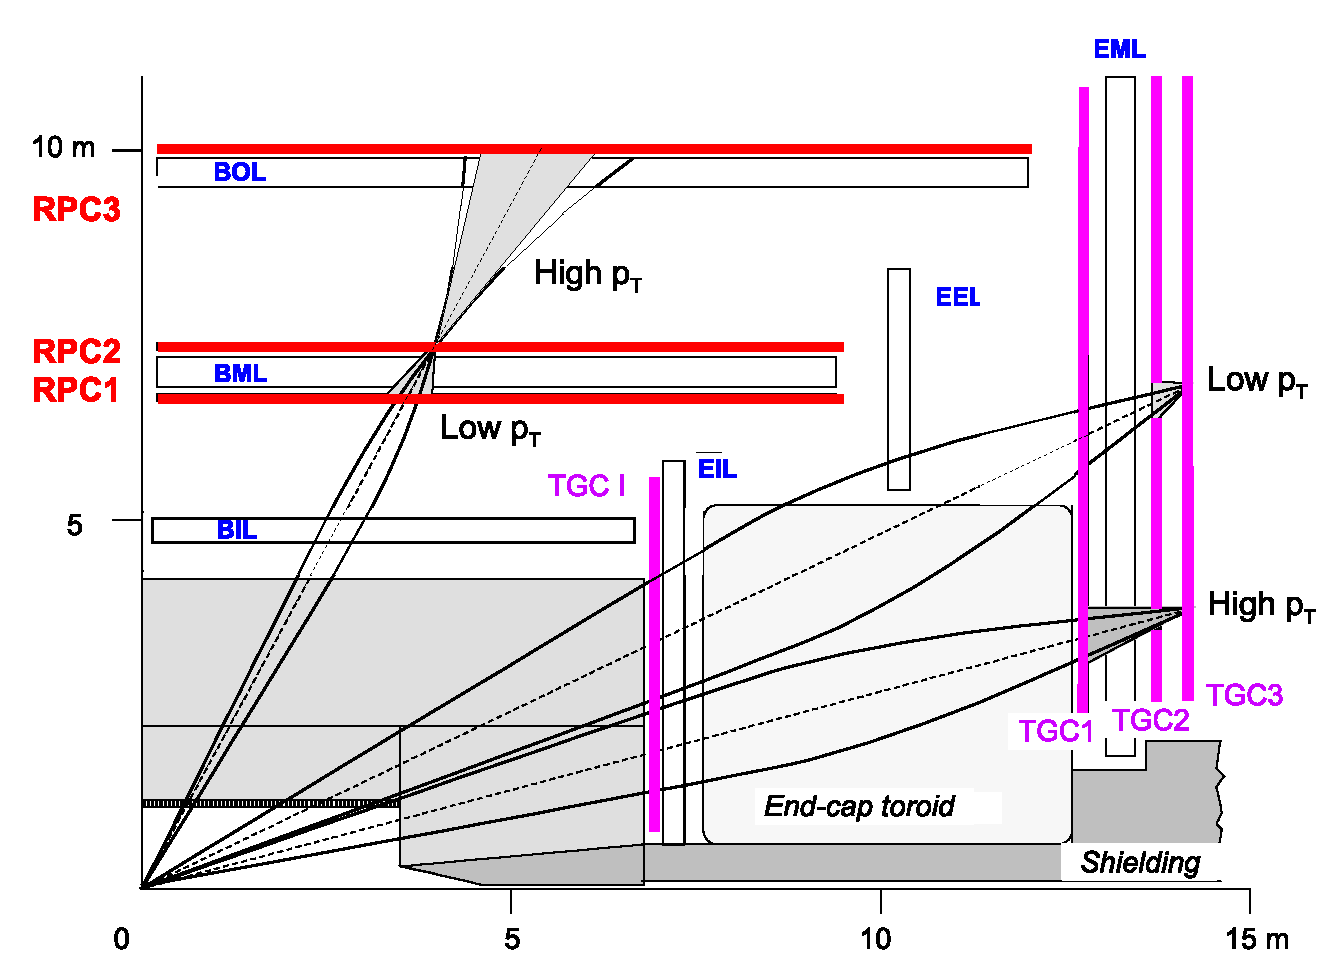
\includegraphics[width=0.8\textwidth]{figures/Atlas/RPC_TGC_schematics}
\end{center}
\caption[Schematic of muon trigger chambers]{Placement of the RPC and TGC layers is shown. RPC layers 1 and 2 book-end the middle MDT layer, and RPC layer 3 lies just outside the outermost MDT layer. TGC layers 1 and 2 surround MDT wheel 2 while TGC layer 3 is just beyond that. An additional TGC layer is placed just inside the end-cap toroid~\cite{ATLAS}.}
\label{fig:muon_trigger}
\end{figure}

In the forward region, the TGC faces several challenges: the end-cap sees ten times the radiation in the barrel, and no bending of muon tracks is provided as the chambers lie outside the end-cap toroidal magnet. To fulfill the triggering requirements, high granularity in $\eta$ and quick response time is achieved with the TGC, using identical principles to those in the multi-wire proportional chambers of the CSC. The gap is filled with a highly-quenching gaseous mixture of 55\,\% CO$_2$ and 45\,\% n-C$_5$H$_{12}$ (n-pentane), while the 50\,$\mu$m diameter gold plated tungsten anode wires are kept at a 2.9\,kV potential. In the TGC, the wire-to-cathode distance of 1.4\,mm is smaller than the wire-to-wire distance of 1.8\,mm, lending to a quick response. High spatial resolution is achieved by varying the number of wires grouped per read-out channel. 

\begin{figure}[tbp]
\begin{center}
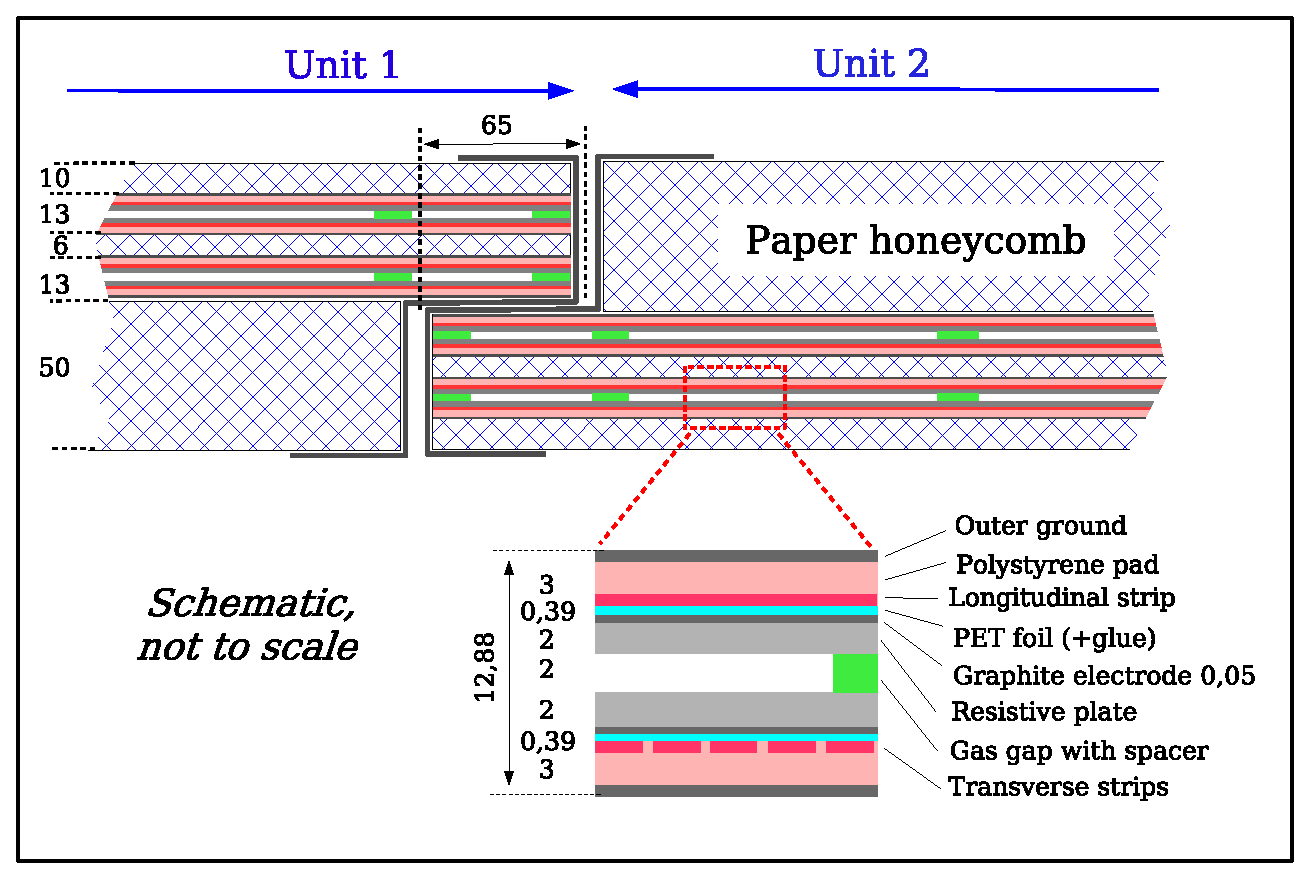
\includegraphics[width=0.4\textwidth]{figures/Atlas/RPC_structure}
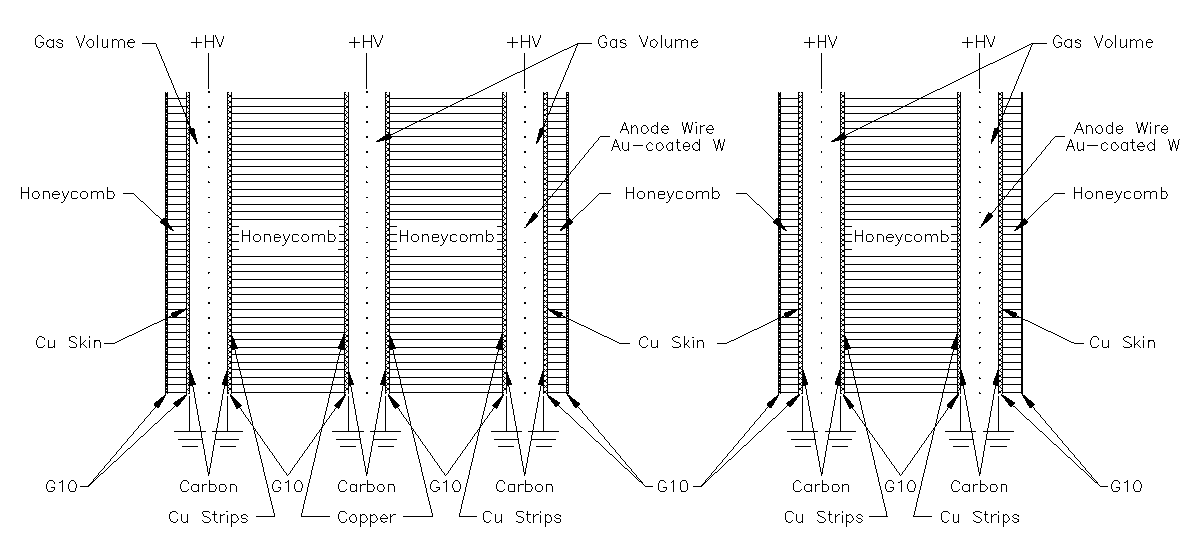
\includegraphics[width=0.59\textwidth]{figures/Atlas/TGC_structure}
\end{center}
\caption[Structure of the muon Resistive Plate Chambers and Thin Gap Chambers]{(left) Structure of the wireless resistive plate RPC and (right) multi-wire proportional chamber TGC~\cite{ATLAS}.}
\label{fig:muon_trigger_struct}
\end{figure}

The structure of the RPC and TGC modules are shown in~\Fig{\ref{fig:muon_trigger_struct}}. The triggering chamber $\phi$ measurement is used if the $\eta$ coordinate for a muon track in nearby MDT and triggering chambers match. There is a vanishing probability of more than one uncorrelated muon track per event in an MDT/triggering chamber pair.
%\footnote{If there are two uncorrelated tracks, it is ambiguous how to match the tracks.} 
However, two correlated, nearby muon tracks could appear from the decay of low mass particles, in which case the track must be matched with the ID. To control for fake rates, coincidence in both $\eta$ and $\phi$ is required for hits in all three triggering layers. In the RPC (TGC), layer 2 (layer 3) is used as a ``pivot-plane'' when determining triggering thresholds. A line from the IP to a hit in the pivot-plane is used as a reference for a straight-trajectory particle. Low (6-9\,\GeV) and high (9-35\,\GeV) \pt thresholds are determined by comparing the slope between hits in specified layers\footnote{
	The low (high) \pt threshold in the RPC is determined by measuring the slope between hits in layer 2 and layer 1 (layer 2 and layer 3). This slope is compared to the slope determined by the path from the IP to the hit in the pivot plane, layer 2. The trigger is passed if the difference in slope is above a threshold.
} and the slope of the reference straight-trajectory particle as depicted in~\Fig{\ref{fig:muon_trigger}}.


%%
\section{Forward Detectors}
Besides the detector systems already mentioned, three forward detectors are present, primarily to aid in luminosity measurements. The locations and coverage of the forward detectors are described in~\Tab{\ref{tab:fwd_loc}}. 

\begin{table}[tbp]
\begin{center}
\begin{tabular}{llr}
\hline
\textbf{Detector} & \textbf{Coverage} & \textbf{Dist. from IP} \\
&&($|z|$ [m]) \\\hline\hline
LUCID & $5.6 < |\eta| < 5.9$ &17\\
ZDC    & $8.3<|\eta|$ &140\\
ALFA  & $10.6 < |\eta|<13.5$ &240\\\hline
\end{tabular}
\end{center}
\caption[Location of forward detectors]{Location and coverage of the forward detectors.}
\label{tab:fwd_loc}
\end{table}

The Luminosity Measurement Using Cherenkov Integrating Detector (LUCID) measures inelastic $pp$ collisions in the forward region and primarily monitors the relative online luminosity.
%\footnote{A measure of the absolute luminosity is also possible with LUCID, but requires calibration either from simulation or other detector measurements.}. 
LUCID consists of 20 aluminum cones directed at the IP filled with C$_4$F$_{10}$ at 1.2-1.4\,bar, in order to measure Cherenkov radiation\footnote{
	Radiation emitted when charged particles travel through a dielectric medium faster than the phase velocity of light in that medium.
} from incident particles. By assuming the number of particles detected is proportional to the number of interactions in the bunch crossing, LUCID is able to measure $\mu$ in order to calculate the luminosity.  In Run II, the original LUCID detector was upgraded to LUCID-2~\cite{LUCID_2} to deal with several challenges: fast aging from a large total integrated luminosity, constraints on electronics from 25\,ns bunch crossings, increased particle fluxes saturating PMTs and counting algorithms, and a new beam pipe material\footnote{
	Moving from stainless steel to aluminum approximately increases the flux of particles through LUCID by a factor of four.
}. The new design no longer uses a gas, but rather quartz windows as the Cherenkov medium.


The Zero-Degree Calorimeter (ZDC) measures neutrons in the extremely forward region of $|\eta|>8.3$ for heavy-ion collisions.
%\footnote{ZDC can also help with low luminosity $pp$ collisions by measuring diffractive processes and aiding beam tuning.} 
ZDC plays an important role in determining the centrality
%\footnote{Centrality of heavy-ion collisions describes the amount of overlap between two colliding nuclei.} 
of heavy-ion collisions, since the number of neutrons in the forward region is highly correlated with the centrality of the collision. ZDC is a sampling calorimeter with tungsten absorber plates perpendicular to the beam line threaded with quartz rods, which serve as the active medium measuring Cherenkov radiation. 

The Absolute Luminosity For ATLAS (ALFA) detector determines the absolute cross section and luminosity by measuring elastic $pp$ scattering at an extremely small angle of 3\,$\mu$rad. The optical theorem relates the scattering amplitude in the extremely forward region to the exact cross section. The detector consists of scintillating fibres and sits inside a Roman pot
%\footnote{The name comes from the CERN Rome group at the Intersecting Storage Rings accelerator in the 1970's who first developed the technique.} 
which can be moved as close as 1\,mm from the beam axis. The detector can only be used during special runs with low emittance and high $\beta^{*}$.
%\footnote{Low emittance corresponds to particles confined tightly together with nearly the same momentum. High $\beta^{*}$ corresponds to a long tapering of the cross section of the beam, or low ``squeeze''.}

%%%
\iffalse
%%%
During the LHC shut down period between 2015 and 2016, part of the ATLAS Forward Proton (AFP) Detector~\cite{AFP_TDR} was installed, while the rest was installed between 2016 and 2017. The AFP is designed to measure forward protons from inelastic collisions, sitting  at $|z|=206$\,m (tracker) and $|z|=218$\,m (time-of-flight detector). The detectors are placed in Roman pots so they can be moved very close to the beam axis. The time-of-flight detector can help reduce pile-up by accurately determining the vertex position. The tracker sensors and read-out are based on the IBL 3D pixel sensors and FE-I4 chips.  At low luminosities, AFP is sensitive to diffractive events, while at high luminosities it is sensitive to anomalous couplings between photons and $W$ or $Z$ bosons. 
%%%
\fi
%%%

The Beam Conditions Monitor (BCM) helps with monitoring the beam stability and determining the luminosity.  If several proton bunches impact the collimators in front of the detectors, the large instantaneous radiation dose may cause severe damage. Thus, the BCM is designed to monitor the stability using precise time of flight measurements and trigger a beam dump if necessary. BCM modules consist of diamond sensors placed at $|z|=1.8$\,m and $R=5.5$\,cm. In Run-II, the Diamond Beam Monitor (DBM)~\cite{DBM} was added to complement the BCM, which can saturate at instantaneous luminosities of $10^{34}$\,cm$^{-2}$s$^{-1}$. The DBM, located approximately one meter from the IP, adds tracking capabilities with chemical vapor deposition diamond sensors. 


%%
\section{Magnet System}
The ATLAS magnet system~\cite{Magnet_TDR} allows for the measurement of the momentum of charged particles by bending their trajectories. The system consists of a central solenoid magnet, a barrel toroid magnet, and two end-cap toroid magnets, depicted in~\Fig{\ref{fig:mag_layout}}.

\begin{figure}[htbp]
\begin{center}
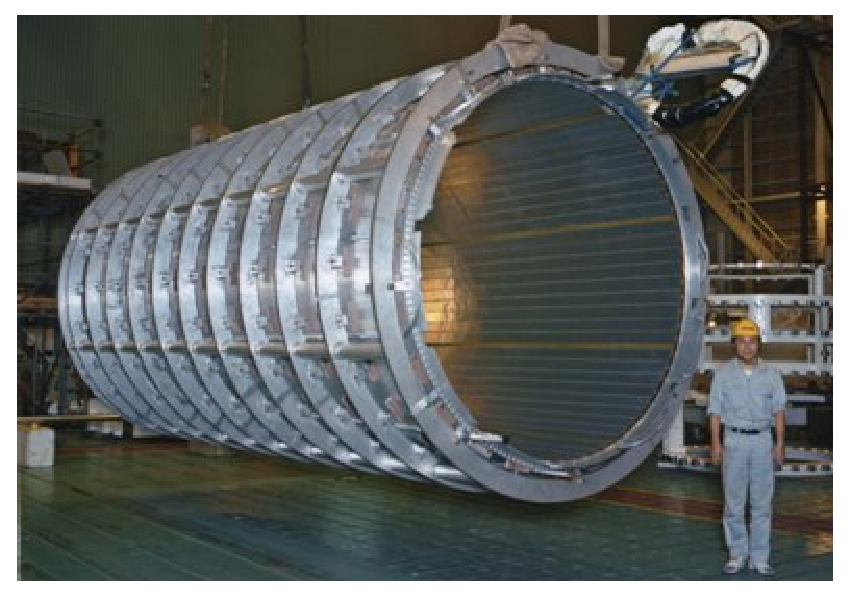
\includegraphics[width=0.48\textwidth]{figures/Atlas/sol_mag}
\includegraphics[width=0.51\textwidth]{figures/Atlas/bar_tor}
\caption[Photo of ATLAS solenoid and barrel toroid magnets]{The ATLAS solenoid magnet (left) after completion of the coil winding and barrel toroid magnets (right) after installation is shown, both next to a physicist for scale~\cite{ATLAS}.}
\label{fig:mag_layout}
\end{center}
\end{figure}

The central solenoid magnet surrounds the ID while sitting in front of the calorimeters. It provides a constant 2\,T axial field for the ID, and is relatively thin at 0.66\,$X_0$, to minimize energy losses and showering of particles before they enter the calorimeter. To minimize the material thickness yet still produce a strong field, the superconducting magnet uses Al-stabilized NbTi conductor wires wound inside an aluminum support. The 5 tonne solenoid magnet has over 9\,km of superconducting wire and measures 5.3\,m along the beam axis, with an inner diameter of 2.46\,m and an outer diameter of 2.56\,m.

%\begin{figure}[htbp]
\begin{wrapfigure}{r}{.51\textwidth}
\begin{center}
\includegraphics[width=0.5\textwidth]{figures/Atlas/atlas-ma-field}
\end{center}
\caption[Magnetic field of barrel toroid magnet]{The magnetic field of the barrel toroid magnet system at $z=0$~\cite{Atlas_mag}.}
\label{fig:atlas_magfield}
\end{wrapfigure}
%\end{figure}

The barrel toroidal magnet system consists of eight identical toroids azimuthally distributed around the beam axis. The system provides on average a 0.5\,T azimuthal field outside the calorimeters, shown in~\Fig{\ref{fig:atlas_magfield}}, to bend muons passing through the MS. The barrel toroid has over 100\,km of superconducting wire, with an envelope that is 25.3\, long with an inner diameter of 9.4\,m and an outer diameter of 20.1\,m.

Two end-cap toroid magnet systems sit on either side of the barrel toroid, to provide on average a 1.0\,T azimuthal field for muons in the end-cap region. The end-cap toroids can be retracted to access the inner subdetectors of ATLAS in the barrel region. The end-cap toroids are composed of eight flat square coils interspaced with keystone wedges. Each end cap toroid measures 5\,m along the beam axis, with an inner diameter of 1.7\,m and an outer diameter of 10.7\,m. 

%%
\section{Trigger and Data Acquisition}
Since data from one raw event is $\mathcal{O}$(1)\,MB\footnote{
	The event size increased from 1.6\,MB in Run-I to 2.4\,MB in Run-II in part due to a 20\,\% increase in read-out channels; however, the event size also depends on the pile-up. 
}, operating at the full LHC design frequency of 40\,MHz (25\,ns bunch spacing) corresponds to a total recording rate near $\mathcal{O}$(10)\,TB/s,
%\footnote{The exact rate fluctuates with the filling scheme, as not every bunch is filled with protons during normal operations.} 
if no filtering is implemented. Due to limitations in processing power and storage in the data acquisition system, however, this rate is intractable. The original design of the Trigger and Data Acquisition (TDAQ) system, utilized in Run-I, consists of a three level triggering system with a final recording rate of approximately 300\,MB/s. In Run-II, nearly all components received an upgrade, to maintain acceptably low \pt thresholds while dealing with increasingly challenging demands: increased center-of-mass energy from 8\,\TeV\,to 13\,\TeV, increased pile-up ($\mu$), decreased bunch spacing interval from 50\,ns to 25\,ns, and increased instantaneous luminosity~\cite{trigger_2015, trigger_evo}. The Run-II TDAQ architecture and parameters are shown in~\Fig{\ref{fig:tdaq_run1_run2_v2}} and~\Tab{\ref{tab:tdaq_run1_run2}}.

\begin{wrapfigure}{r}{.51\textwidth}
\begin{center}
\includegraphics[width=0.49\textwidth]{figures/Atlas/tdaq_run2_v1}
\end{center}
\caption[Trigger and Data Acquisition architecture in Run-II]{The TDAQ architecture was modified in Run-II by consolidating the Level-2 and Event Filter stages into one High Level Trigger stage. The total event rate increased from 600\,Hz in Run-I to 1\,kHz in Run-II, in a more challenging environment, with the help of the upgrades and optimizations implemented~\cite{trigger_evo}.}
\label{fig:tdaq_run1_run2_v2}
\end{wrapfigure}

The first level of the trigger system is a hardware-based Level-1 (L1) trigger which slims the 40\,MHz input event rate to a 100\,kHz output rate.
%\footnote{Although the L1 rate has increased from Run-I, the 100\,kHz output rate is hardware-limited by the read-out capabilities of the ATLAS subdetectors; thus, in future upgrades of the LHC, the trigger architecture and detector read-outs will need upgrades to accommodate the ever-increasing luminosity and $\mu$.} 
The L1 trigger tries to identify high-\pt electrons, photons, muons, jets, and hadronically decaying $\tau$-leptons, as well as large \MET and $E_{\rm T}^{\text{tot}}$. Sums of calorimeter energy deposits from 7000 trigger towers, with an approximate granularity of $\Delta\eta\times\Delta\phi=0.1\times0.1$, are collected by the ``L1Calo'' trigger, while RPC and TGC track information is collected by the ``L1Muon'' trigger.  A ``trigger menu'' consisting of 512 ``trigger items'', logical combinations of trigger inputs from L1Calo and L1Muon, is processed by the Central Trigger Processor (CTP) which produces a trigger decision within 2.5\,$\mu$s. Event data must be buffered while the L1 trigger decision is being formed. The trigger items in the trigger menu can be ``pre-scaled'' so that a predetermined fraction of events passing the trigger item are randomly ignored, thereby reducing the overall trigger rate. The CTP is also responsible for limiting the time between L1 accepts (simple dead time) and a leaky bucket algorithm to limit the number of L1 accepts in a given number of bunch crossings (complex dead time)~\cite{Leaky_bucket}. A detector may issue a ``busy'' signal to the CTP in order to signal that its buffers are full, preventing further L1 accepts until the busy signal is cleared.
\begin{table}[tbp]
\begin{center}
\begin{tabular}{lrr}
\hline
Property & Run-I & Run-II \\\hline\hline
$\sqrt{s}$ [\TeV] & 8 & 13\\
L$_{\text{peak}}$ [$10^{33}$\,cm$^{-2}$s$^{-1}$] & $5.0$ & $13.8$\\
Bunch spacing [ns] & 50 & 25 \\
\# bunches & 1380 & 1380-2700\\
Avg. pile-up & 20.7 & 24.9 \\
Event size [MB] & 1.6 & 2.4 \\
L1 inputs (items) & 160 (256) & 512 (512) \\
L1 rate [kHz] & 70 & 100 \\
Total output rate [kHz (GB/s)] & 0.6 (0.96) & 1.0 (2.4) \\
\hline
\end{tabular}
\end{center}
\caption[Trigger and Data Acquisition parameters in Run-I and Run-II]{Comparison of LHC and TDAQ parameters between Run-I and Run-II (up to 2016). The increased luminosity, center of mass energy, and pile-up required updated algorithms and architecture to address the increased production rate and keep the output rate reasonable.}
\label{tab:tdaq_run1_run2}
\end{table}

Event data is buffered on detector-specific front-end electronics until a L1 trigger decision is received. Upon an L1 accept, the next stage in the data acquisition system is the transfer of the buffered event data to a read out system (ROS) at approximately 240\,GB/s. A data collection (DC) system interfaces with fragments from the ROS to provide requested event information to the next level of the trigger, the High Level Trigger (HLT). 

The second level of the triggering system is the software-based HLT\footnote{The current HLT performs the combined functions of the Run-I Level-2 trigger and Event Filter.}, which reduces the 100\,kHz L1 rate to a final 1\,kHz event output rate, with an average latency of 200\,ms. The HLT uses regions of interest (ROI) identified by the L1 trigger (approximately 2\,\% of the total event data) to access full or partial event information from the ROS through the DC interface. The L1 ROIs seed a system of approximately 2500 ``trigger chains'' in the HLT: a sequence of algorithms which increase in complexity and require more detector information. The HLT has access to full granularity calorimeter information, precision muon measurements, and ID tracking information, all of which is unavailable to the L1 trigger. The HLT utilizes a two-pass approach: a first quick reconstruction rejects the majority of events, and a second slower, more precise reconstruction filters the remaining events. Pending an HLT accept, event data buffered in the ROS is transferred to the Tier-0 storage facilities at CERN at 2.4\,GB/s for full offline event reconstruction. 




%%_______________________
%% METHODS:
%% Object Reconstruction & Id
%% Event Selection
%% Background and Signal Estimation
%%-----------------------
% !TEX root = ../main.tex
%%__________________________________
%% Object Reconstruction 
%% Data/MC, Analysis Strategy
%%----------------------------------

% !TEX root = ../../main.tex
\chapter{Object Reconstruction and Identification}
\label{ch:objreco}

Combining measurements from various ATLAS subdetectors allows for the identification of physics objects like electrons, muons, photons, and hadrons. The trajectory of a particle can be reconstructed by matching position measurements in the calorimeters and MS with track hits in the ID. Converging tracks extrapolated towards the IP identify vertices, and the one with the largest $\sum \pT^2$ for all associated tracks is labeled the primary vertex (PV).  Reconstructed objects are associated to the same interaction when their tracks extrapolate to the PV. In this analysis, the reconstructed objects of interest are: electrons, muons and jets. Additionally, missing transverse energy, $\MET$, is used to identify neutrinos which do not interact with the detector. This chapter describes the selections and algorithms used to identify these physics objects.

%
\section{Electrons}
\label{ch:objreco:el}
Electron objects are reconstructed by matching clusters of EM calorimeter energy deposits to reconstructed tracks in the ID. To build the EM cluster, a sliding window algorithm is used~\cite{sliding_window}. The window is a fixed-size grid of cells, $N_{\eta}\times N_{\phi}$=3\times5, in the middle layer of the LAr calorimeter where approximately $80\,\%$\,of the energy in an EM shower is deposited (\Sect{\ref{ch:atlas:particle_showers}}). For each cell, the energy is summed across all the longitudinal layers, forming a tower. If the transverse energy of the towers in the window is above 2.5\,\GeV\,and is a local maximum, a seed cluster is formed. 

After loose shower shape requirements are applied to the seed clusters, a cone-shaped region of interest (ROI) of $\Delta R<0.3$ from the seed barycenter is defined~\cite{electron_efficiency, electron_efficiency_2016}.  Pattern recognition and track fitting algorithms are then used to match ID tracks to seed clusters. Track seeds from the ID with $\pT>1\,\GeV$\, are tested against pion and electron pattern recognition algorithms, and are required to reside in a cluster ROI. A track fit is performed twice to extrapolate the ID track to the calorimeter, using the track momentum or the cluster momentum, and is required to be near the cluster. If either succeeds, a final optimized track reconstruction is performed using a Gaussian Sum Fitter (GSF)~\cite{gsm_filter}. 
%A summary of the track reconstruction and cluster matching parameters is shown in~\Tab{\ref{tab:el_cl_tr}}.

An electron candidate is formed if there is at least one ID track matched to the seed cluster. The EM cluster is then rebuilt by summing energy in a grid of $3\times 7$ cells in each layer, starting in the middle layer. After calibrations and corrections are applied, the four-momentum of the electron candidate is calculated using the energy measurement of the EM cluster and the $\eta$ and $\phi$ measurements from the track.

%\begin{table}[tb]
%\begin{center}
%\begin{tabular}{l|c|c|c|c}
%\hline\hline
%\textbf{Reconstruction} & \multicolumn{2}{c|}{$\Delta\phi_{\textrm{EM cluster}}$} & \multicolumn{2}{c}{$\Delta\eta_{\textrm{EM cluster}}$}  \\\cline{2-5}
%\textbf{Method}& Curve toward & Curve away & non-TRT-only & TRT-only \\\hline
%Track Momentum & $<0.2$ & $<0.05$ & $<0.05$ & --- \\\cline{2-5}
%Cluster Momentum & $<0.1$ & $<0.05$ & $<0.05$ & --- \\\hline
%\multicolumn{1}{l}{\textbf{Final}} &\multicolumn{4}{c}{\,} \\\hline
%$\quad$ non-TRT-only (GSF) & \multicolumn{2}{c|}{$<0.1$} & \multicolumn{2}{c}{---} \\\cline{2-5}
%$\quad$ TRT-only & $<0.03$ & $<0.02$ & --- & $<0.35$\\\hline\hline
%\end{tabular}
%\caption[Calorimeter cluster track matching requirements]{Requirements on the proximity of the extrapolated tracks to the calorimeter cluster seeds are shown for several reconstruction methods. The $\Delta\phi$ requirements depend on if the reconstructed track curves toward or away from the seed cluster. If extrapolation with either the track momentum or cluster momentum succeeds, a final track reconstruction is performed. For non-TRT-only tracks, the final reconstruction uses an optimized Gaussian Sum Filter (GSF) algorithm~\cite{gsm_filter}. }
%\label{tab:el_cl_tr}
%\end{center}
%\end{table}



Background objects like hadronic jets, non-prompt electrons from photon conversions, and semi-leptonic decays of hadrons with heavy quarks can ``fake'' an electron signature and be reconstructed at this stage as an electron candidate~\cite{electron_efficiency}. A multivariate analysis (MVA) technique takes into account several cluster and track variables to create a likelihood (LH) identification for each candidate as either signal or background. Different working points balancing signal efficiency with background rejection are provided as shown in~\Fig{\ref{fig:el_id_eff}}; in this analysis, the ``LooseLH'' and ``TightLH'' are considered, where TightLH is a subset of LooseLH. The LooseLH working point has very high signal efficiency and mostly offers light flavor jet discrimination. The TightLH working point has a lower signal efficiency, but additionally rejects photon conversions and heavy flavor jets.

In addition to the discrimination due to the LH identification, further suppression of background electrons is provided with isolation criteria~\cite{electron_efficiency_2016}. A real electron from, for example, a $W$ boson decay, will be produced in relative isolation while jets, converted photons, and other fake electrons will be accompanied by nearby energy deposits. Isolation is calculated both from the calorimeter EM cluster, and from the ID track. Calorimeter isolation, $E_{\rm T}^{\textrm{cone} 0.2}$, calculates the sum of transverse energy ($E_{\rm T}$) in a cone of $\Delta R<0.2$ around the 
\begin{wrapfigure}{r}{.6\textwidth}
\begin{center}
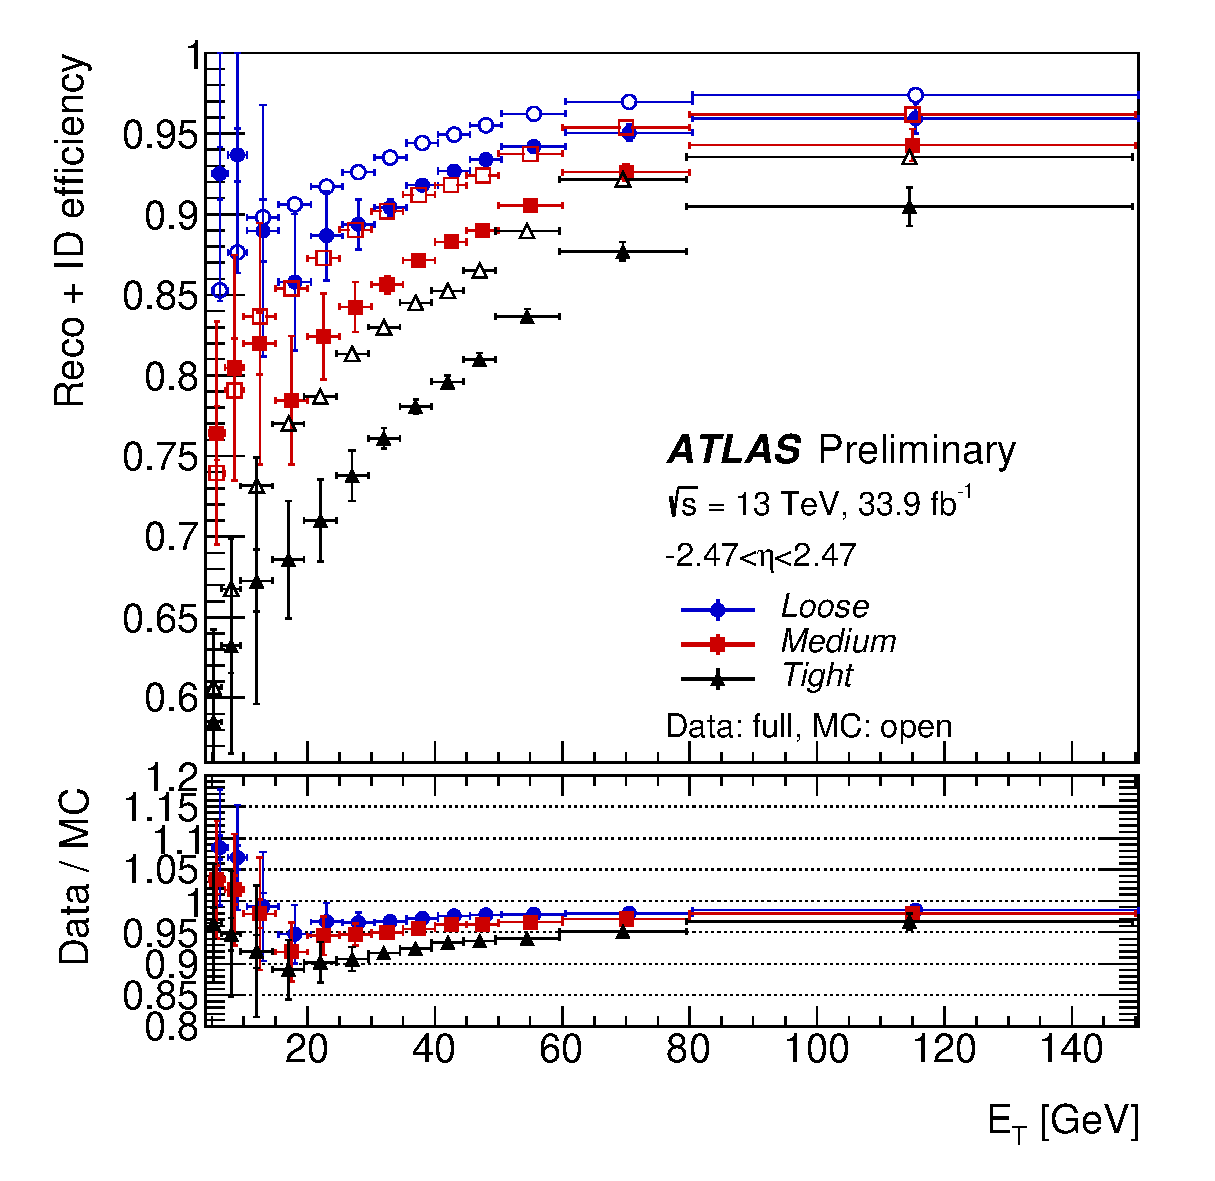
\includegraphics[width=.59\textwidth]{figures/ObjectReconstruction/el_id_eff}
\end{center}
\caption[Electron reconstruction and identification efficiencies]{The reconstruction and identification efficiencies for signal electrons is presented as a function of transverse energy for several working points~\cite{el_id_eff}.}
\label{fig:el_id_eff}
\end{wrapfigure}
electron center, and subtracts the $5\times7$ cell window contribution from the electron. Track isolation, $\pT^{\textrm{varcone} 0.2}$, calculates the sum of transverse momentum for quality tracks in a variable cone of size $\Delta R< \textrm{min}(0.2, 10\,\GeV/E_{\rm T})$ centered around and excluding the electron track. Working points using calorimeter and/or track based isolation are provided for either 1) a specific efficiency with variable cuts or 2) fixed cut values. The ``LooseTrackOnly'' and ``FixedCutTight'' isolation working points are used in this analysis. The LooseTrackOnly working point only uses the ID track based isolation for a constant $99\,\%$\, efficiency. The FixedCutTight working point cuts at $E_{\rm T}^{\textrm{cone} 0.2}/E_T < 0.06$ and $\pT^{\textrm{varcone} 0.2}/E_T < 0.06$.

The identification and isolation working points are optimized for electrons coming from the PV. This analysis additionally requires the recommended cuts on longitudinal ($z_0$) and transverse ($d_0$) impact parameters to verify the reconstructed electron is associated with the PV. Electrons are required to have $|\eta|<2.47$, excluding the calorimeter transition region between $1.37<|\eta|<1.52$, where the uncertainties can be large due to poor resolution. Finally, a minimum transverse momentum is required to avoid trigger turn-on curves, as discussed in~\Ch{\ref{ch:event_selection}}. This analysis uses two types of electrons, ``signal'' and ``veto'', which are defined and summarized in~\Tab{\ref{tab:lep_def}}. Veto electrons are used to avoid overlap with similar analyses with distinct final states. 

\begin{table}[htbp]
\begin{center}
\begin{tabular}{l|c|c|c|c}
\hline\hline
\multicolumn{1}{c|}{\textbf{Cut}} & \multicolumn{2}{c|}{\textbf{Electron Definition}} &  \multicolumn{2}{c}{\textbf{Muon Definition}} \\\cline{2-5}
& Veto & Signal & Veto & Signal \\\hline
\pt [\GeV] & $>7$ & $> 27$  & $>7$ & $> 27$ \\\hline
$|\eta|$ & \multicolumn{2}{c|}{$<2.47\notin[1.37, 1.52]$} & $<2.7$ & $<2.5$ \\\hline
Identification & LooseLH & TightLH & Loose & Medium  \\\hline
\vbox{\hbox{\strut Isolation}\hbox{\strut}} & \vbox{\hbox{\strut LooseTrack-}\hbox{\strut Only}} & \vbox{\hbox{\strut FixedCutTight}\hbox{\strut}} & \vbox{\hbox{\strut LooseTrack-}\hbox{\strut Only}} & \vbox{\hbox{\strut FixedCutTight-}\hbox{\strut TrackOnly}}\\\hline
$|d_0/\sigma(d_0)^{BL}|$ & \multicolumn{2}{c|}{$<5$} & \multicolumn{2}{c}{$<3$}\\\hline
$|z_0\sin\theta|$ [mm]& \multicolumn{4}{c}{$< 0.5$}  \\\hline\hline
\end{tabular}
\caption[Electron and muon object definitions]{The object definitions for electrons and muons used in this analysis are shown. Veto leptons are defined to reduce overlap with similar final state searches. }
\label{tab:lep_def}
\end{center}
\end{table}
%
\section{Muons}
Muon objects are reconstructed by matching track candidates independently created in the MS and ID~\cite{muon_eff}. In the MS, algorithms create segments by matching hits aligned in the bending plane between multiple layers. If multiple track segments match in different layers, a track candidate is formed. 

Using combinations of information from the ID, calorimeters, and MS, four types of muon candidates are defined. In decreasing priority, they are:
\begin{itemize}
	\item \underline{Combined (CB)}: The full muon track is reconstructed, starting in the MS and extrapolating towards the ID.
	\item \underline{Segment Tagged (ST)}: The ID track is extrapolated towards the MS, where it must match at least one MDT/CSC track segment (useful for low-\pT muons).
	\item \underline{Calo Tagged (CT)}: The ID track is extrapolated to the calorimeter, where it matches an energy deposit (useful in the region $|\eta|<0.1$ where the MS has no coverage).
	\item \underline{Stand Alone (SA)}: A MS track not matched to an ID track, but extrapolated close to the IP, is used to recover muons in the range $2.5<|\eta|<2.7$ that has poor ID coverage.
\end{itemize}

Background objects, such as decaying pions and kaons, can be reconstructed as a ``fake'' muon candidate. Using the four types of muon candidates, and additional cuts based on track and calorimeter based variables, working points for muon identification are created to balance signal efficiency with background rejection. In this analysis, the ``Medium'' and ``Loose'' identification working points are used, corresponding to approximate efficiencies of 96.1\,\% and 98.1\,\%, respectively. The Medium working point only uses CB and SA candidates, while the Loose working point considers all four types. 

Muon isolation is performed analogously to electron isolation: track-based and calorimeter-based isolation measurements are used to create working points with either 1) efficiency based variable cuts or 2) fixed cuts. The track-based muon isolation, $\pt^{\textrm{varcone} 0.3}$, uses a slightly larger cone, $\Delta R < 0.3$, with respect to the electron case.  In this analysis, ``LooseTrackOnly'' and ``FixedCutTightTrackOnly'' isolation working points are used. The LooseTrackOnly working point has a constant $99\,\%$\, efficiency. The FixedCutTightTrackOnly requires $\pt^{\textrm{varcone} 0.3}/\pT < 0.06$.

Finally, as with electrons, two types of muon objects are defined, ``signal'' and ``veto''. Recommended $\pT$, $\eta$, and PV association cuts are additionally placed on the muon objects, whose definitions are summarized in~\Tab{\ref{tab:lep_def}}. 

%
\section{Jets}
Hadronization of quarks from the initial hard scatter event, or subsequent hadronic decays of unstable particles ($W\ra q\overline{q}'$, $Z\ra q\overline{q}$), creates showers of lower energy particles, called jets, in the detector. Jets are formed by clustering nearby energy deposits in the calorimeter and matching the cluster with ID tracks. 

Topologically connected three dimensional cell clusters, or ``topo-clusters''~\cite{topo_cluster}, are used as constituents in the formation of a jet. Unlike the sliding-window calorimeter cluster seeds used for electrons, topo-clusters can have variable sizes. A topo-cluster is seeded if the energy of a cell is four standard deviations above the noise level ($E_{\textrm{cell}}>4 \sigma_{\textrm{cell}}^{\textrm{noise}}$), and connected cells are added to the cluster if $E_{\textrm{cell}}>2 \sigma_{\textrm{cell}}^{\textrm{noise}}$. 

The anti-$k_{\rm T}$ jet reconstruction algorithm~\cite{anti_kt_algo} is a sequential combination algorithm used in this analysis to combine topo-clusters into jet objects. A distance parameter is defined in~\Eqn{\ref{eq:anti_kt}}.
\begin{eqnarray}
\label{eq:anti_kt}
d_{ij} &=& \textrm{min}\left(\frac{1}{p_{\rm T,i}^2},\frac{1}{p_{\rm T,j}^2}\right)\frac{\Delta R_{ij}^2}{R^2}  \\
d_{iB} &=& \frac{1}{p_{\rm T,i}^2} 
\end{eqnarray}
The distance $d_{ij}$ measures the distance between two topo-clusters, while $d_{iB}$ measures the distance between a topo-cluster and the beam line. The distance parameter, $R$, roughly defines the size of the jet. The clustering procedure iteratively finds the smallest distance among all constituents. If the smallest distance is between two clusters, $d_{ij}$, the clusters are combined and the procedure continues. If it is between a cluster and the beam axis, $d_{iB}$, the cluster is defined as a jet and removed from the collection of remaining constituents. The distances are then recalculated and more jets are found until there are no remaining clusters. The anti-$k_{\rm T}$ algorithm tends to combine high-\pT constituents first and produces a roughly conical jet. ID tracks are matched with jets through a procedure known as ``ghost association''~\cite{ghost_assoc}. In effect, tracks are identified as particles with infinitesimal momentum and included in the clustering process. Their negligible momentum ensures the final jet clusters are not affected, but will include the tracks. In this analysis, ``small-R jets'' ($j$) and ``large-R jets'' ($J$), corresponding to $R=0.4$ and $R=1.0$, are used.

The energies of calorimeter jets are corrected for PU with a $\mu$-dependent subtraction. Additionally, a ``jet energy scale" (JES) response correction~\cite{jet_energy_measurement}  is applied to accurately calibrate both EM and hadronic showers. The JES aims to correct for the non-compensating nature of the calorimeters (hadrons have a lower detector response with respect to EM objects like electrons and photons), and energy loss in regions of the detector without measuring instruments. Small-R jets in this analysis use a simple JES scheme, called ``EM+JES'', in which the jets are measured at the EM scale\footnote{
	 The EM scale means the energy of an EM shower will be correctly measured.
} and a scale factor is applied based on the $\pT$ and $\eta$ measurements of the jet. For large-R jets, a local cluster weighting (LCW) procedure applies calibrations at a topo-cluster level, according to whether the cluster corresponds to a hadronic or EM energy deposit.  In this ``LCW+JES" scheme, jets are reconstructed from the locally calibrated clusters and a final JES scale factor is applied (smaller than in the EM+JES scheme). 
%
\subsection{Small-R Jets}
\label{ch:objectReconstruction:smallr}
Small-R jets ($R=0.4$) are used in this analysis to identify both VBF jets, and jets from $b$-quark decays. In VBF candidate events, the initial quarks, which radiate vector bosons, have a small deflection and hadronize into two jets with a large separation in $\eta$. Jets with $b$-hadrons, called $b$-jets, are useful for identifying candidate events from top quark pair decays ($t\bar{t}$). Candidate $b$-jets (VBF jets) must have $\pT>20\,\GeV$\, (30\,\GeV) and $|\eta| < 2.5$ (4.5).

Although a uniform PU subtraction is applied, local deviations may create PU jets. These jets can originate from both QCD effects (from a single PU vetex) and stochastic effects (contributions from multiple vertices). To reject both types of PU jets, a jet vertex tagger (JVT)~\cite{jvt} is used to assign jets to the PV. The JVT is a two-dimensional likelihood discriminant which factors in tracking and vertex information. For this analysis, the 92\,\% efficiency working point is used for jets with $\pT<60\,\GeV$\,and $|\eta|<2.4$. A residual 2\,\% of PU jets remain at this efficiency.

A multivariate $b$-tagging algorithm called MV2~\cite{b_jet} is used to tag small-R jets that contain $b$-hadrons. MV2 takes as input several $b$-tagging algorithms based on the impact parameter, secondary vertex reconstruction, and full decay chain reconstruction. The MV2 algorithm uses a boosted decision tree with background composition from $c$-jets (light-jets) of 7\,\% (93\,\%). Light-jets refer to jets from gluons or $u, d,$ or $s$ quarks. For this analysis, the 85\,\%\,efficiency $b$-tagging working point is used. The inverse of the corresponding mis-tag rate, called the rejection ratio, is 3.1 (33) for $c$-jets (light-jets)~\cite{b_jet_opt}. VBF candidate jets are required to fail $b$-tagging. A summary of the small-R jets definitions is shown in~\Tab{\ref{tab:small_j_def}}.

\begin{table}[htbp]
\begin{center}
\begin{tabular}{l|c|c}
\hline\hline
\multicolumn{1}{c|}{\textbf{Cut}} & \multicolumn{2}{c}{\textbf{Small-R Jet Definition}} \\\cline{2-3}
& $b$-jet Candidate & VBF jet Candidate  \\\hline
Algorithm & \multicolumn{2}{c}{Anti-$k_{\rm T}$ $R=0.4$}  \\\hline
Energy Calibration & \multicolumn{2}{c}{EM+JES} \\\hline
\pt [\GeV] &$>20$&$>30$\\\hline
$|\eta|$ &$<2.5$&$<4.5$\\\hline
\vbox{\hbox{\strut Pileup Removal}\hbox{\strut (JVT 92\,\% efficiency)}} & \multicolumn{2}{c}{\vbox{\hbox{\strut if\, $\pT<60\,\GeV$}\hbox{\strut \&\& $|\eta|<2.4$}}}  \\\hline
$b-$tag (MV2c10 85\,\% efficiency)& pass & fail \\\hline\hline
\end{tabular}
\caption[Small-R jet object definition]{The object definitions for small-R jets used in this analysis are shown.}
\label{tab:small_j_def}
\end{center}
\end{table}


%
\subsection{Large-R Jets}
\label{ch:objectReconstruction:larger}
Large-R jets ($R=1.0$) are used in this analysis to identify boosted hadronically decaying vector bosons.  Jets from the two-body decays of boosted vector bosons have a substructure typically absent from decays of gluons and light quarks~\cite{boost_trim}. To elucidate the substructure differences, grooming techniques remove soft contributions to the jet. In particular, this analysis uses a grooming technique called trimming, depicted in~\Fig{\ref{fig:jet_trim}}. Jet trimming further aims to improve the jet mass resolution by removing contamination from initial state radiation (radiation from the incoming hadrons), multiple parton interactions (further interactions among the partons after the hadron collision), and PU interactions. 
The trimming procedure in this analysis involves the following steps:
\begin{itemize}
	\item Re-cluster the large-R jet ($J$) constituents into ``sub-jets'' with the anti-$k_{\rm T}$ algorithm with distance parameter $R=0.2$.
	\item Remove sub-jets if $p_{\rm T}^{\textrm{sub-jet}}< 0.05\times p_{\rm T}^{J}$.
	\item Recombine the surviving sub-jets into a final trimmed jet.
\end{itemize}
\begin{figure}[tbp]
\begin{center}
\includegraphics[width=.8\textwidth]{figures/ObjectReconstruction/jet_trim}
\caption[Jet trimming illustration]{The jet trimming procedure is illustrated. In this analysis, sub-jets are created with the anti-$k_{\rm T}$ algorithm with distance parameter $R_{\textrm{sub}}=0.2$, and the fractional \pT threshold is set at $f_{\textrm{cut}}=0.05$~\cite{boost_trim}.}
\label{fig:jet_trim}
\end{center}
\end{figure}

Even with trimming, jet mass resolution can suffer in the high-\pT regime from a loss of angular information when multiple highly boosted decay products are reconstructed as a single topo-cluster. A track mass, $m_{\textrm{track}}$, based on ID charged particle tracks can be used to improve the mass resolution~\cite{jet_track_mass}. The track mass is calculated by ghost associating ID tracks with $\pT>0.4\,\GeV$ to the large-R jet, and then summing the masses associated with all matched tracks. To correct for the missing neutral particle contribution to $m_{\textrm{track}}$, a ratio of the calorimeter-based to track-based transverse momentum is applied to the track mass. The resulting quantity, called the track-assisted mass, is shown in~\Eqn{\ref{eq:m_ta}}.
\begin{equation}
m_{\textrm{TA}} \equiv m_{\textrm{track}}\times\frac{p_{\rm T}^{\textrm{calo}}}{p_{\rm T}^{\textrm{track}}}
\label{eq:m_ta}
\end{equation}

To take advantage of both the calorimeter and track-assisted mass, a weighted sum, minimizing the jet mass resolution and called the combined mass, is defined in~\Eqn{\ref{eq:m_comb}}~\cite{jet_comb_mass}.
\begin{equation}
m_{\textrm{comb}} \equiv w_{\textrm{calo}}\times m_{\textrm{calo}} + w_{\textrm{track}}\times m_{\textrm{TA}}
\label{eq:m_comb}
\end{equation}
In this analysis, $m_{\textrm{calo}}$ and $m_{\textrm{TA}}$ are taken to be uncorrelated (reflecting an approximate 10\,\%\,correlation for $\pT > 1\,\TeV$). The weights in~\Eqn{\ref{eq:m_comb}} can thus be expressed in terms of the estimated jet mass resolution, $\sigma_{\textrm{calo}}$ ($\sigma_{\textrm{TA}}$) for $m_{\textrm{calo}}$ ($m_{\textrm{TA}}$), as shown in~\Eqn{\ref{eq:m_comb_uncorr}}.
\begin{equation}
m_{\textrm{comb}} = \frac{\sigma_{\textrm{calo}}^{-2}m_{\textrm{calo}} +  \sigma_{\textrm{TA}}^{-2}m_{\textrm{TA}}}{\sigma_{\textrm{calo}}^{-2}+\sigma_{\textrm{TA}}^{-2}}
\label{eq:m_comb_uncorr}
\end{equation}
The estimated jet mass resolutions are calculated as a function of \pT and $\eta$. The improvement in jet mass resolution of the combined mass is shown in~\Fig{\ref{fig:m_comb_res}}. The jet transverse momentum is also re-scaled to be compatible with the combined mass, as shown in~\Eqn{\ref{eq:jet_pt_comb}}.
\begin{equation}
p_{\rm T}^{\textrm{comb}} \equiv p_{\rm T}^{\textrm{calo}}\times\frac{m_{\textrm{comb}}}{m_{\textrm{calo}}}
\label{eq:jet_pt_comb}
\end{equation}
In the rest of this thesis, the combined mass and combined transverse momentum of the large-R jet will be referred to as $m(J)$ and $\pT(J)$ respectively. To ensure a complementary overlap between calorimeter and tracking information, large-R jets are required to have $|\eta|<2.0$. This search focuses on boosted $W$ or $Z$ bosons; thus, the large-R jet is required to have $\pT(J)>200\,\GeV$ and $m(J)>50\GeV$.
\begin{figure}[tbp]
\begin{center}
\subfloat[]{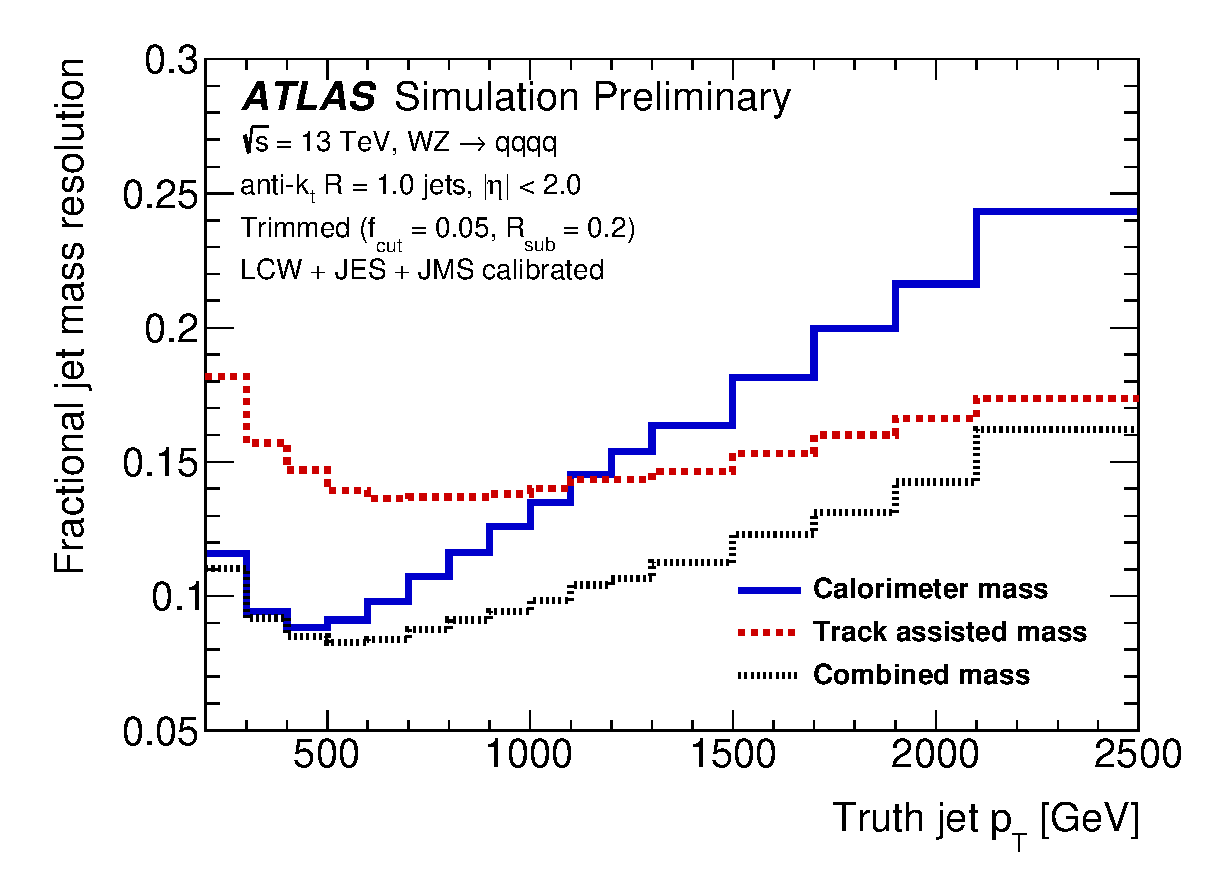
\includegraphics[width=.49\textwidth]{figures/ObjectReconstruction/m_comb_res}\label{fig:m_comb_res:a}}
\subfloat[]{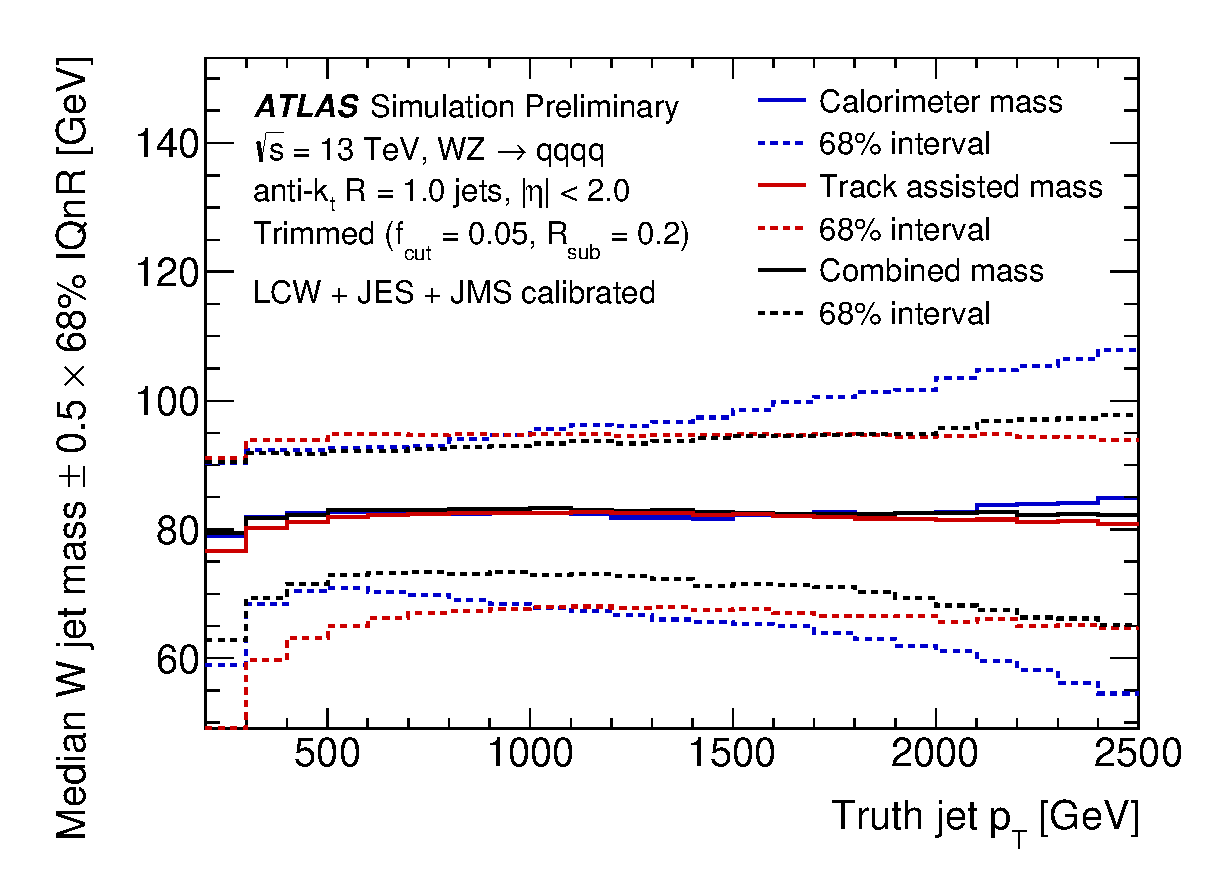
\includegraphics[width=.49\textwidth]{figures/ObjectReconstruction/med_reconst_w_mass}\label{fig:m_comb_res:b}}
\end{center}
\caption[Performance of combined mass for large-R jets]{Three jet mass definitions are used to compare \protect\subref{fig:m_comb_res:a} the fractional jet mass resolution and \protect\subref{fig:m_comb_res:b} the median reconstructed jet mass, for simulated boosted $W$ or $Z$ bosons, as a function of truth \pT. The combined mass improves jet mass resolution for $250\,\GeV<\pT<2.5\,\TeV$ and $|\eta|<2.0$~\cite{jet_track_mass}.}
\label{fig:m_comb_res}
\end{figure}


To further differentiate jets due to a two-body decay of boosted $W$ or $Z$ bosons from QCD jets due to single partons, a substructure variable ($D_2^{\beta=1}$), based on the ratio of generalized two and three point energy correlation functions, is introduced~\cite{d2_one, d2_two}, as shown in~\Eqnrange{\ref{eq:en_corr_func}}{\ref{eq:d2_def}}. 
\begin{eqnarray}
e_2^{\beta} & = & \frac{1}{\pT^2(J)}\sum_{1\leq i<j\leq n_j}\pT^i\pT^j\Delta R_{ij}^{\beta}  \label{eq:en_corr_func} \\
e_3^{\beta} & = & \frac{1}{\pT^2(J)}\sum_{1\leq i<j<k\leq n_j}\pT^i\pT^j\pT^k\Delta R_{ij}^{\beta}\Delta R_{ik}^{\beta}\Delta R_{jk}^{\beta} \\
D_{2}^{\beta=1} & = & \frac{e_3^{\beta=1}}{\left(e_2^{\beta=1}\right)^3} \label{eq:d2_def}
\end{eqnarray}
For $n_j$ constituents in the jet, $\pT^i$ is the transverse momentum of the i$^{\textrm{th}}$ constituent, and $\Delta R_{ij}$ is the previously defined angular separation between the i$^{\textrm{th}}$ and j$^{\textrm{th}}$ constituents.

A boson tagging algorithm, called SmoothedWZTagger~\cite{smoothed_wz_tagger}, identifies large-R jets as either a $W$ or $Z$ boson decay, based on the large-R jet combined mass and $D_2^{\beta=1}$ substructure variable, at fixed signal efficiency working points of $50\,\%$\, and $80\,\%$. The selections are optimized in \pT bins and a smoothing function is fit to the resulting mass-window and $D_2^{\beta=1}$ threshold cuts, as depicted in~\Fig{\ref{fig:smooth_cuts}}. A summary of the large-R jet definition is presented in~\Tab{\ref{tab:large_jet_def}}.
\begin{figure}[htbp]
\begin{center}
\subfloat[]{\includegraphics[width=.5\textwidth]{figures/ObjectReconstruction/MassWindow_newWZTagger}\label{fig:smooth_cuts:a}}
\subfloat[]{\includegraphics[width=.5\textwidth]{figures/ObjectReconstruction/D2UpperCut_newWZTagger}\label{fig:smooth_cuts:b}}
\caption[Boson tagger mass and substructure cuts]{The SmoothedWZTagger selections cuts for \protect\subref{fig:smooth_cuts:a} the combined mass window and \protect\subref{fig:smooth_cuts:b} the upper-cut on $D_2^{\beta=1}$, are shown as a function of \pT for both the $50\,\%$\,and $80\,\%$ efficiency working points. The $50\,\%$\,($80\,\%$) efficiency working point corresponds to a background rejection factor of 45-75 (11-13) and 50-70 (9-13) for $W$ and $Z$ bosons respectively.}
\label{fig:smooth_cuts}
\end{center}
\end{figure}
\begin{table}[htbp]
\begin{center}
\begin{tabular}{l|c}
\hline\hline
\textbf{Cut} &\textbf{Large-R Jet Definition} \\\hline
Algorithm & Anti-$k_{\rm T}$ $R=1.0$  \\\hline
Grooming & Trimming with $R_{\textrm{sub-jet}}=0.2$, $f_{\textrm{cut}}=0.05$ \\\hline
Energy Calibration & LCW+JES \\\hline
\pt [\GeV] &$>200$\\\hline
$|\eta|$ &$<2.0$\\\hline
Mass [\GeV] & $>50$ \\\hline
Boson Tagging & SmoothedWZTagger \\\hline\hline
\end{tabular}
\caption[Large-R jet definition]{The object definition for large-R jets used in this analysis.}
\label{tab:large_jet_def}
\end{center}
\end{table}


%
\section{Missing Transverse Energy}

Neutrinos produced in collisions pass through ATLAS without leaving energy deposits in the calorimeters, or tracks in the ID and MS. Since the colliding protons have no initial momentum transverse to the beam line, momentum conservation implies that the vector sum of the transverse momentum of all the final state particles should also be zero. Deviations from zero can indicate the presence of a non-interacting particle, like a neutrino, in the final state.  In \Eqn{\ref{eq:met_eq}}, the calculation of \MET is summarized as the negative vector sum of all reconstructed objects, and additional ``soft terms'' corresponding to tracks from the PV that are not matched to reconstructed objects.
\begin{eqnarray}
E^{\textrm{miss}}_{x(y)} &=& - \sum\limits_{e\in\{\textrm{electrons}\}} p_{x(y)}^{e}  - \sum\limits_{\mu\in\{\textrm{muons}\}} p_{x(y)}^{\mu}  - \sum\limits_{j\in\{\textrm{jets}\}} p_{x(y)}^{j}   - \sum\limits_{s\in\{\textrm{soft terms}\}} p_{x(y)}^{s} \nonumber \\
\MET & = & \sqrt{\left(E_x^{\textrm{miss}}\right)^2+ \left(E_y^{\textrm{miss}}\right)^2}
\label{eq:met_eq}
\end{eqnarray}
The use of soft terms that have ID tracks consistent with the PV ignores possible contributions from neutral particles. A calorimeter-based soft term, using topologically connected clusters unassociated with reconstructed particles, can be used to measure these contributions. However, the track-based soft terms offer better \MET resolution and are less pile-up dependent~\cite{met_perf}. As a result, the track-based soft terms are used in this analysis to reconstruct \MET. Photons and hadronically decaying taus are not used in this analysis, and are reconstructed as jets in the \MET calculation. 

In this analysis, the \MET is identified as the transverse momentum of the neutrino, $\pT^{\nu}$. To determine the $z$ component of the neutrino momentum, the $W$ boson from the $W\ra\ell\nu$ decay is constrained to be exactly on-shell with $m(W\ra\ell\nu)=80.4\,\GeV$. Using this constraint, a quadratic equation for the neutrino $p_z$ can be solved. If a solution is complex, the real part is taken, and if two unique solutions exist, the smallest in absolute value is taken. A more detailed discussion is presented in~\App{\ref{ch:neutrinopz}}.

%
\section{Overlap Removal}
As electrons, muons, and jets use a combination of tracking and calorimeter measurements, a single collection of energy deposits and tracks may be reconstructed independently as several physics objects. To remove any ambiguity, a procedure is defined to prioritize which reconstructed objects are kept and which are discarded.

\begin{itemize}
\item If there is a shared ID track between an electron candidate and a muon candidate, the electron is removed. In this case, the MS track from the muon candidate cannot be due to an electron. 
\item Next, if there is a small-R jet and electron candidate with $\Delta R(j,e)<0.2$, the small-R jet is removed since the reconstructed jet does not differentiate between hadronic and EM showers. However, the electron is removed if $0.2<\Delta R(j,e)<\textrm{min}(0.4,0.04+10\,\GeV/\pT(e))$. Electrons reconstructed near the edge of a jet are most likely from non-prompt decays of jet constituents. The sliding cone, with maximum size $R=0.4$ at low $\pT(e)$, recovers boosted prompt electrons that are close to the edge of jets. 
\item If there is a large-R jet and electron with $\Delta R(J,e)<1.0$, the large-R jet is removed. 
\item If a muon and small-R jet satisfy $\Delta R(j,\mu)<0.2$, and either 1) the jet has fewer than two tracks or 2) $\pT(\mu)/\pT(j)>0.5$ and $\pT(\mu)/\sum\pT(\textrm{tracks})>0.7$, the jet is discarded. This indicates the jet is most likely from the calorimeter energy loss of a muon. If the jet is not removed, a sliding cone is used to remove the muon if $\Delta R(j,\mu)<\textrm{min}(0.4,0.04+10\,\GeV/\pT(\mu))$. Similar to the electron case, boosted muons sufficiently far from the jet center are kept, while lower \pT muons likely from non-prompt decays near the jet edge are removed. 
\item There is no overlap removal between muons and large-R jets, as muons are unlikely to deposit enough calorimeter energy to be reconstructed as a jet with $\pT>200\,\GeV$.
\end{itemize}


% !TEX root = ../../main.tex
\chapter{Analysis Strategy}
\label{ch:analysisStrategy}
As motivated in~\Ch{\ref{ch:limitations}}, the boosted diboson resonance is a valuable probe of BSM physics. The semi-leptonic final state capitalizes on the properties of both hadronic and leptonic decays of weak bosons. In a $pp$ collider, the presence of an isolated high energy lepton in conjunction with \MET is a discerning feature that is useful for rejecting many QCD background processes. Requiring the other boson to decay hadronically takes advantage of a larger branching ratio, while mitigating the signal loss associated with the signal efficiencies of large-R jet boson tagging (\Sect{\ref{ch:objectReconstruction:larger}}).

In~\Sect{\ref{ch:analysisStrategy:evt_top}}, the boosted regime and the event topology of the search is described. The main SM background processes are detailed in~\Sect{\ref{ch:analysisStrategy:bkgs}}. Finally, the estimation of these SM backgrounds, as well as the benchmark signal models, through the use of Monte Carlo simulations is outlined in~\Sect{\ref{ch:analysisStrategy:sig_bkg_model}}. 

%
\section{Event Topology}
\label{ch:analysisStrategy:evt_top}
When hadronically decaying objects produced at the LHC have large transverse momentum, $\pt$, with respect to their rest mass, their decay products in the detector are very collimated, and they are referred to as boosted objects~\cite{lhc_boosted}. The search focuses on a heavy resonance decaying to a pair of boosted weak bosons: a $W$ boson decaying leptonically and either a $W$ or $Z$ boson decaying hadronically. The leptonically decaying $W$ is reconstructed as an isolated electron or muon, with a neutrino identified as \MET. The search considers topologies where the two quarks in the hadronic $W/Z$ decay cannot be separately resolved with the standard small-R jet reconstruction. Instead, they are reconstructed as a single boosted large-R jet with distance parameter $R=1.0$. 

%wrap was here

For diboson resonances produced just above threshold approximately at rest, the two decaying daughter bosons will have nearly equal \pT, as expressed in~\Eqn{\ref{eq:pt_larger}}. For each boson, the distance between the decay products is shown in~\Eqn{\ref{eq:dr_larger}}~\cite{LargeRjet_kin}. 
\begin{eqnarray}
\pt(V)&\simeq& m(WV)/2 \label{eq:pt_larger} \\
\Delta R(q,q)&\simeq&2m(V)/\pt(V) \label{eq:dr_larger}
\end{eqnarray}
When this separation becomes comparable to the distance parameter of reconstructed small-R jets ($R=0.4$), the reconstructed jets will partially or fully overlap, leading to degraded reconstruction efficiency and energy reconstruction. \Eqn{\ref{eq:dr_larger}} shows that, for SM weak bosons with $\pT(V)\simeq 200\,\GeV$, most of the hadronic activity can be recovered by the large-R jet. 
\begin{wrapfigure}{r}{.61\textwidth}
	\begin{center}
		\includegraphics[width=.6\textwidth]{figures/AnalysisStrategy/h_boosted_resolved_2}
		\caption[Boosted and resolved regimes]{Representation of the boosted and resolved regimes as a function of $\Delta R(q,q)$ between the two quarks in the large-R jet.}
		\label{fig:boosted_regime}
	\end{center}
\end{wrapfigure}
For weak bosons with $\pT(V)\simeq 200\,\GeV$, this corresponds approximately to resonances with $m(WV)>500\,\GeV$. In \Fig{\ref{fig:boosted_regime}}, the boosted and resolved regimes are shown, separated by $\Delta R(q,q)\simeq 0.8$ between the two quarks in the hadronically decaying boson.  The angular separation of the quarks in the hadronically decaying $W$ boson from a simulated HVT $Z'$ signal (\Sect{\ref{ch:analysisStrategy:sig_bkg_model}}) for several mass points are shown in \Fig{\ref{fig:dr_qq}}. 


\begin{figure}[t!bh]
	\begin{center}
		\subfloat[]{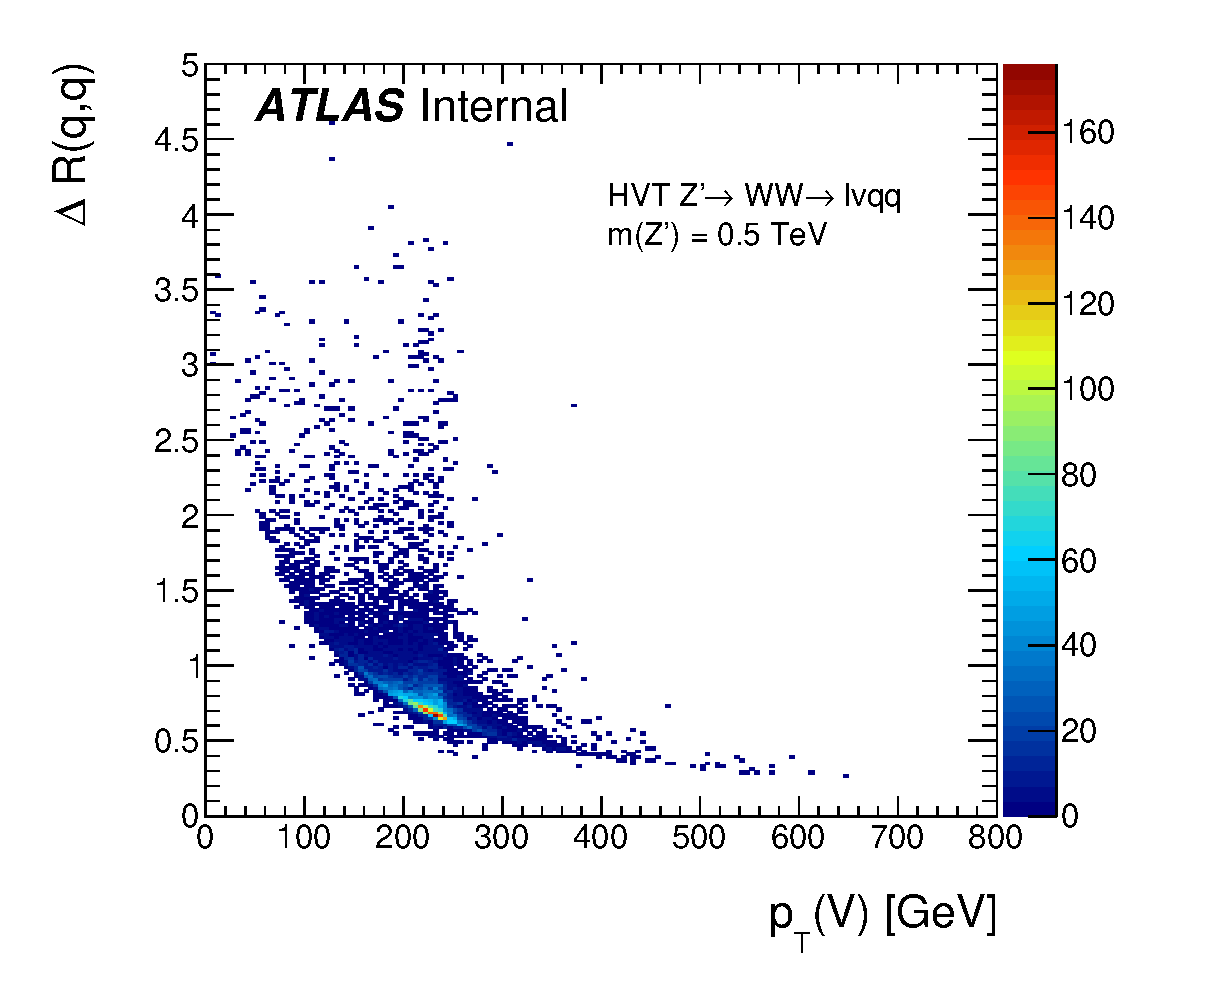
\includegraphics[width=.5\linewidth]{figures/AnalysisStrategy/h_DR_qq_W_500GeV}\label{fig:dr_qq_a}}
		\subfloat[]{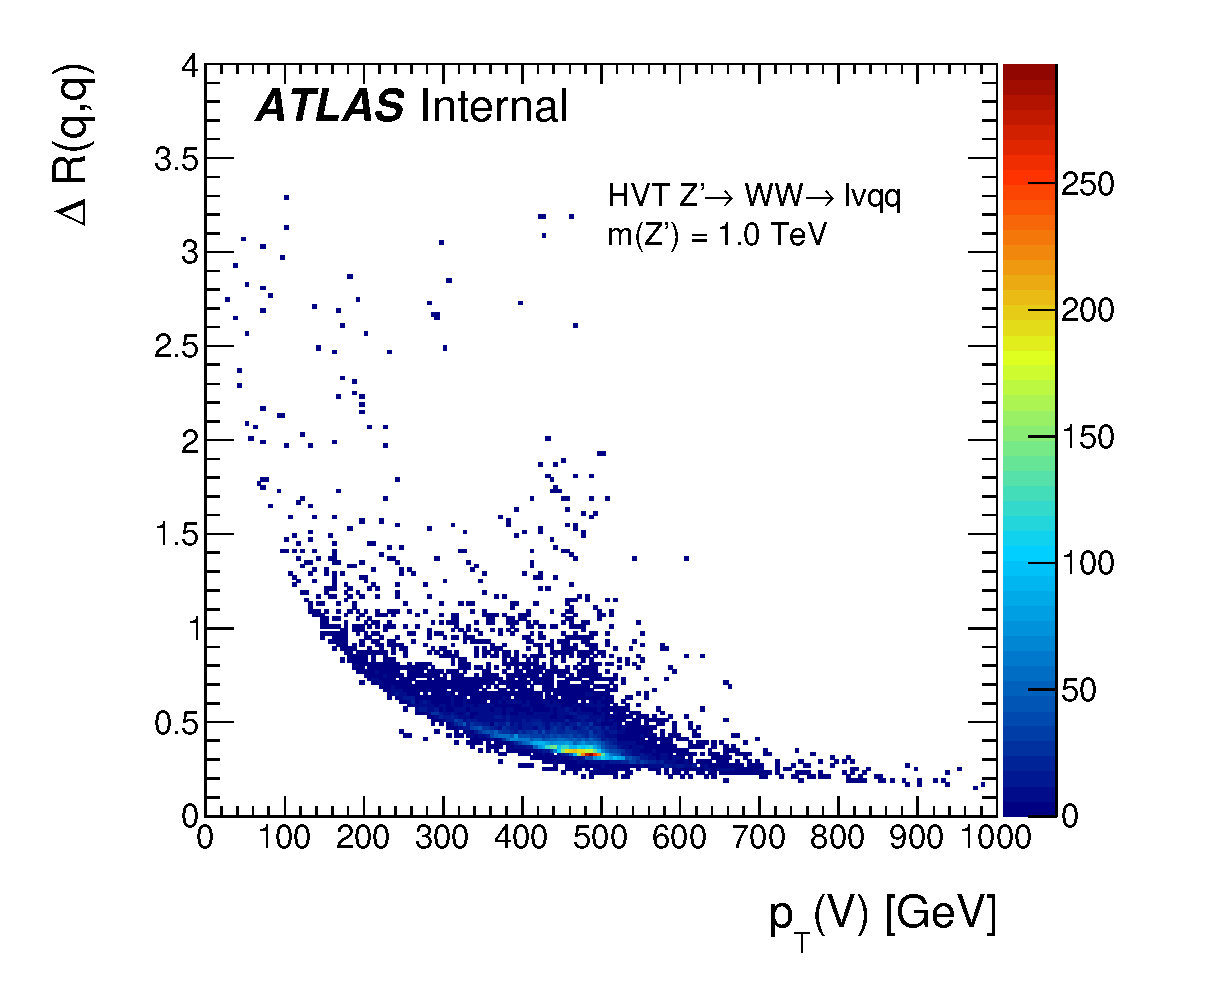
\includegraphics[width=.5\linewidth]{figures/AnalysisStrategy/h_DR_qq_W_1000GeV}\label{fig:dr_qq_b}}\\
		\subfloat[]{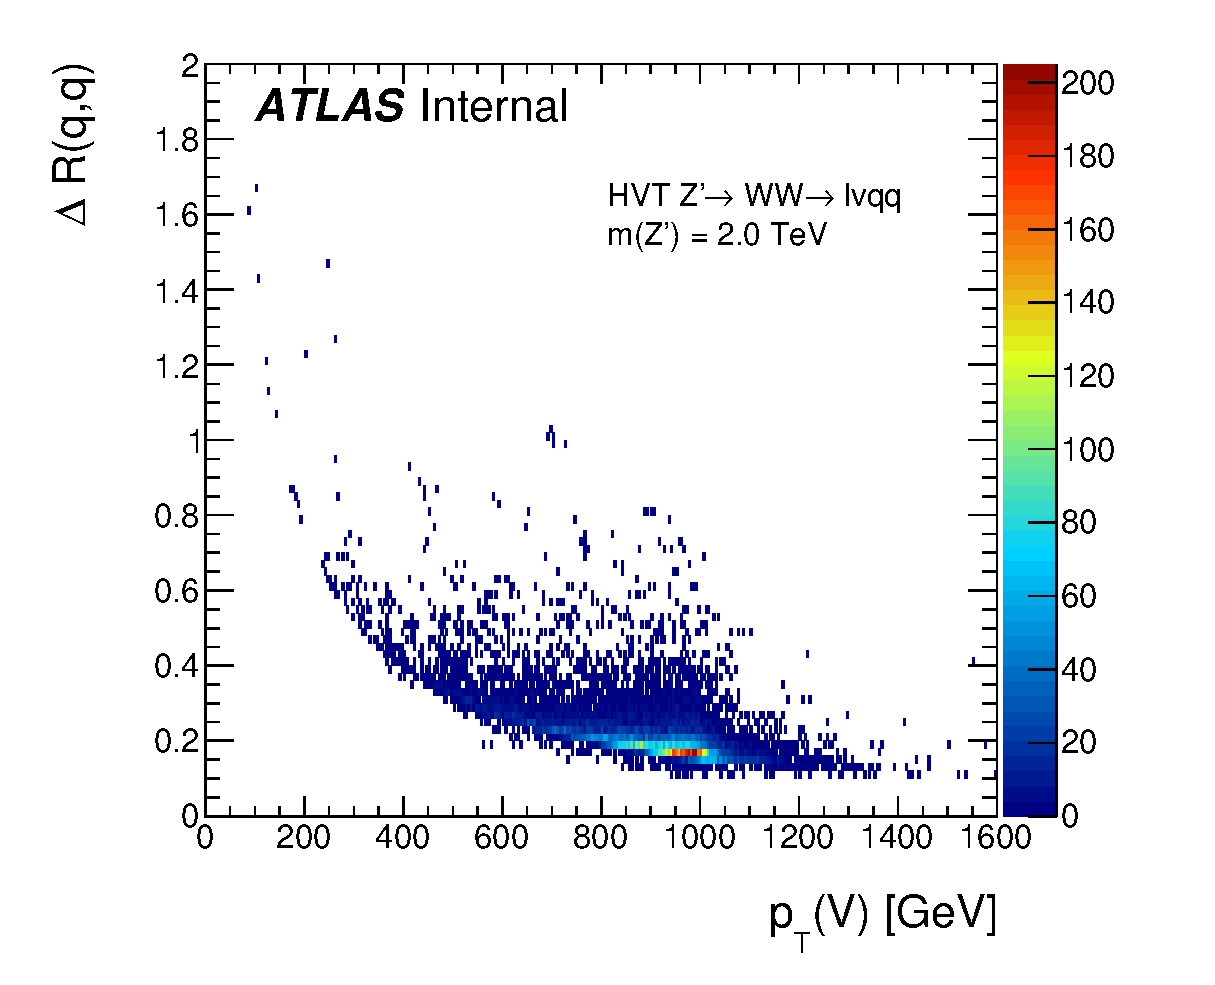
\includegraphics[width=.5\linewidth]{figures/AnalysisStrategy/h_DR_qq_W_2000GeV}\label{fig:dr_qq_c}}
		\subfloat[]{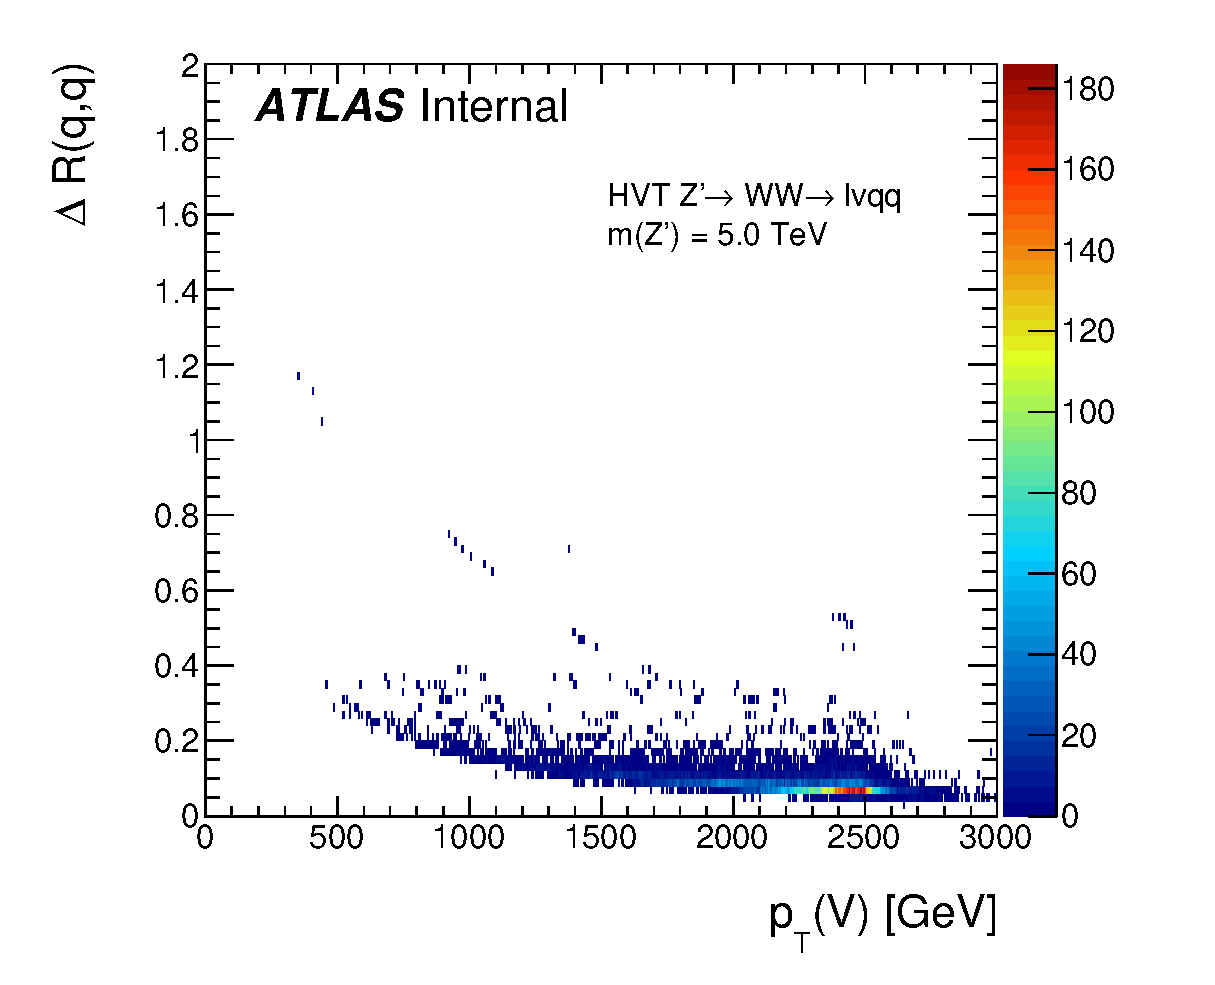
\includegraphics[width=.5\linewidth]{figures/AnalysisStrategy/h_DR_qq_W_5000GeV}\label{fig:dr_qq_d}}\\
		\caption[Separation of quarks as function of boson \pt]{Distribution of $\Delta R(q,q)$ vs $\pt(V)$ for HVT $Z'$ signal masses of \protect\subref{fig:dr_qq_a} 500 GeV, \protect\subref{fig:dr_qq_b} 1.0 TeV, \protect\subref{fig:dr_qq_c} 2.0 TeV, and \protect\subref{fig:dr_qq_d} 5.0 TeV.}
		\label{fig:dr_qq}
	\end{center}
\end{figure}


The search is split according to the signature of the production mechanism. In VBF production, the initial state quarks radiating vector bosons characteristically  hadronize with a large separation in $\eta$. These events are distinguished from gluon-gluon fusion and quark-quark fusion production by the presence of two additional small-R jets ($R=0.4$). The two event topologies of this analysis are depicted in~\Fig{\ref{fig:event_topology}}.

\begin{figure}[tb]
\begin{center}
\subfloat[]{\includegraphics[width=0.49\textwidth]{figures/AnalysisStrategy/event_topology}\label{evt_topology:a}}\hfill
\subfloat[]{\includegraphics[width=0.49\textwidth]{figures/AnalysisStrategy/vbf_topology}\label{evt_topology:b}}
\caption[Diagram of event topologies]{The event topologies for \protect\subref{evt_topology:a} quark-quark fusion or gluon-gluon fusion, and \protect\subref{evt_topology:b} vector boson fusion (VBF). In both topologies, the heavy resonance decays to a central $W$ boson, further decaying leptonically ($W\ra \ell \nu$), and a central $V=W, Z$ further decaying hadronically ($W, Z\ra qq$). The neutrino, $\nu$, in the leptonic decay is reconstructed as missing transverse energy, $\MET$, while the hadronically decaying $V$ is reconstructed as a single large-R jet ($R=1.0$), denoted by $J$. In the case of VBF, two small-R jets ($R=0.4$) with a large separation are also present.}
\label{fig:event_topology}
\end{center}
\end{figure}




%
\section{Main Backgrounds}
\label{ch:analysisStrategy:bkgs}
In the SM, there are various processes which can produce or be reconstructed as the same final state as a semi-leptonic diboson resonance. In order to make an accurate interpretation of the data, these backgrounds must be understood and estimated. Those backgrounds which reproduce the exact final state ($\ell\nu qq$) are called irreducible backgrounds, and cannot be completely eliminated by improved selections. Other backgrounds which are reconstructed as the same final state, due to detector and reconstruction inefficiencies, are called reducible backgrounds, and can be significantly reduced with appropriate selections. Leading order Feynman diagrams of the main backgrounds considered in this search are depicted in~\Fig{\ref{fig:bkg_feyn_lo}}.

The most significant SM background in this analysis is the non-resonant production of a leptonically decaying $W$ boson ($W\ra\ell \nu$) in association with one or more quarks and gluons. The associated quarks and gluons hadronize and are reconstructed as jets; thus, this background is denoted by \Wjets. The QCD jets in this background have a non-resonant mass spectrum, and a different substructure with respect to a hadronically decaying weak boson of the signal. By taking advantage of boson tagging techniques (\Sect{\ref{ch:objectReconstruction:larger}}), the contamination of this background can be reduced. 

The second largest SM background comes from non-resonant top-antitop quark pair production, denoted by \ttbar. The semi-leptonic final state can be reproduced through the decay $t\bar{t} \ra bW^+\bar{b}W^- \ra b\bar{b}l\nu q\bar{q}'$. A decay of a top quark to a lighter down-type quark ($s$, $d$) is strongly suppressed.
%($<10\,\%$).  Much smaller, should I find a number?
The \ttbar background is thus characterized by the presence of $b$-jets in association with the final state. The use of $b$-tagging (\Sect{\ref{ch:objectReconstruction:smallr}}) can improve \ttbar rejection if any $b$-jets lie outside the reconstructed large-R jet.  For both \Wjets and \ttbar backgrounds, the normalization is estimated in dedicated control regions, as described in~\Sect{\ref{ch:eventSelection:srcr}}, using a fit described in~\Ch{\ref{ch:stats}}. 

A single leptonically decaying $Z$ boson ($Z\ra \ell\ell$) in association with jets is also a SM background for the search, denoted by \Zjets. Unlike the \Wjets background, \Zjets can only reproduce the semi-leptonic final state if one of the leptons is incorrectly reconstructed, and is thus reducible. A strict requirement on the number of leptons in the final state can significantly reduce this background.

In addition to the production of a top-antitop quark pair, the electroweak production of a single top quark, denoted \Singlet, can reproduce the semi-leptonic final state. In the $s$-channel and $t-$channel production, the final state is reproduced if the top quark decays leptonically through a $W$ boson. In the $Wt$-channel, a top quark is produced in association with a $W$. As with \ttbar, detecting the presence of additional $b$-tagged jets can help reduce the \Singlet background.

Finally, the non-resonant SM production of two weak bosons, denoted by SM dibosons, must be estimated. 

The non-resonant QCD production of multiple jets (multijet) has an extremely large cross section. Contamination from this background can occur if some of the jets are incorrectly reconstructed as leptons or involve decays with non-prompt leptons, and the reconstructed \MET is too large from detector inefficiencies. Since the modeling of the multijet background is difficult, due to the large rejection rate of fake leptons, the multijet contribution is estimated with a data driven approach. A control region with an enhanced expected QCD contribution (looser lepton selection, low \MET) is used to extract the shape of the multijet distribution. By requiring $\MET>100\,\GeV$ and a cut on $\MET/\pT(W\ra e\nu)$ (\Ch{\ref{ch:event_selection}}), the multijet background can be effectively suppressed, and is estimated to have a negligible impact on this search. More details can be found in~\App{\ref{ch:qcd}}.

\begin{figure}[tbp]
\centering
\begin{minipage}{.32\linewidth}
	 \subfloat[]{
		\feynmandiagram [small, horizontal=a to b, tree layout] {
			a --[gluon, edge label =\(g\)] b,
			b -- [fermion, edge label=\(t\)] c,
			b -- [anti fermion, edge label=\(\bar{t}\)] d, 
			c -- [boson] c1 [particle=\(W^+\)],   
			c -- [fermion] c2 [particle=\(b\)],
			d -- [boson] d1 [particle=\(W^-\)], 
			d -- [anti fermion] d2[particle=\(\bar{b}\)],
		};\label{fig:bkg_feyn_lo:a}}
\end{minipage}
\begin{minipage}{.32\linewidth}
    \subfloat[]{
       \feynmandiagram [small, horizontal=i1 to f2] {
			i1 [particle=\(q\)] -- [fermion] a -- [gluon] f2 [particle={\(g\)}],
			a -- [fermion] b,
			i2 [particle=\(\bar{q}'\)] -- [anti fermion] b -- [boson] f1 [particle={\(W/Z\)}],
			i1 -- [draw=none] i2,
			f1 -- [draw=none] f2
		}; \label{fig:bkg_feyn_lo:b}} \\
	\subfloat[]{
 	   \feynmandiagram [small, horizontal=a to b] {
			i1 [particle=\(q\)] -- [fermion] a -- [fermion] i2 [particle={\(\bar{q}'\)}],
			a -- [boson, edge label={\(W, Z\)}] b,
			f1 [particle=\(W\)] -- [boson] b -- [boson] f2 [particle={\(Z, W\)}],
		}; \label{fig:bkg_feyn_lo:c}}    
\end{minipage}
\begin{minipage}{.32\linewidth}
    \subfloat[]{
       \feynmandiagram [small, horizontal=i1 to f2] {
			i1 [particle=\(b\)] -- [fermion] a -- [fermion] f2 [particle={\(t\)}],
			a -- [boson, edge label=\(W\)] b,
			i2 [particle=\(q\)] -- [fermion] b -- [fermion] f1 [particle={\(q'\)}],
			i1 -- [draw=none] i2,
			f1 -- [draw=none] f2
		}; \label{fig:bkg_feyn_lo:d}} \\
	\subfloat[]{
 	   \feynmandiagram [small, horizontal=a to b] {
			i1 [particle=\(b\)] -- [fermion] a -- [gluon] i2 [particle={\(g\)}],
			a -- [fermion] b,
			f1 [particle=\(W\)] -- [boson] b -- [fermion] f2 [particle={\(t\)}],
		}; \label{fig:bkg_feyn_lo:e}}    
\end{minipage}
\caption[Selected leading order Feynman diagrams for background processes]{Selected leading order Feynman diagrams for the main background processes considered in this search. \protect\subref{fig:bkg_feyn_lo:a} \ttbar (one $W$ decays leptonically) can be reduced by tagging $b$-jets, \protect\subref{fig:bkg_feyn_lo:b} \Wjets and \Zjets backgrounds can be reduced with the help of boson tagging in the large-R jet, \protect\subref{fig:bkg_feyn_lo:c} SM diboson production will have a non-resonant mass spectrum, \Singlet production in the \protect\subref{fig:bkg_feyn_lo:d} $t$-channel and \protect\subref{fig:bkg_feyn_lo:e} $Wt$-channel can be reduced by tagging $b$-jets.}
\label{fig:bkg_feyn_lo}
\end{figure}


%
\section{Signal and Background Modeling}
\label{ch:analysisStrategy:sig_bkg_model}
Monte Carlo (MC) techniques are used to simulate both signal and background processes, and to model the response of the ATLAS detector. MC generated events are then used to optimize the event selection, and to compare the collected data with the estimated SM background contributions. A full list of the signal and background MC samples used in this analysis is available in~\App{\ref{ch:samples}}.
% Do I need this? 
%Precise modeling of estimated background contributions is vital in order to maintain high sensitivity to new physics.

Proton collisions at the LHC involve both hard (perturbative QCD) and soft (non-perturbative QCD) processes. As such, the event generation procedure involves splitting the full calculation into several smaller stages with different methods of evaluation. The first ``matrix element'' step involves calculating the initial hard scattering process of a fixed number of incoming and outgoing partons, using perturbative methods at leading-order (LO), or next-to-leading order (NLO) in powers of $\alpha_s$, the strong coupling constant. The subsequent showering of the outgoing partons, and hadronization of the color connected constituents, is modeled next. Finally, the ``underlying event'' (UE), comprised of processes not originating from the hard scatter event, are modeled and overlaid on the event. This includes initial and final state radiation from the incoming and outgoing partons in the hard scatter event, and additional interactions of the fragments of the colliding protons.

For all simulated samples, \textsc{Pythia} 8.186~\cite{pythia8} is used to model additional inelastic $pp$ interactions in the same bunch crossing, denoted as pile-up (PU). These PU interactions are then overlaid on the generated events. The number of PU events is reweighted with the standard ATLAS ``PileupReweightingTool'' so that the distribution of the average number of interactions per bunch crossing, $\langle\mu\rangle$, in the MC samples matches that in data. The particles in the simulated events are then propagated through the detector using the \textsc{GEANT4}~\cite{geant4} based detector simulation. The standard ATLAS reconstruction software~\cite{atlas_sim} then produces an event output in the same format as data. Physics objects are created using the same algorithms described in~\Ch{\ref{ch:objreco}}.

%
\subsection{Monte Carlo Generators}
The collisions at the LHC often involve the associated production of multiple hard (high-\pT) jets. The task of modeling the hard jet multiplicity can be accomplished either at the matrix element evaluation stage, or the showering stage. \textsc{Pythia} and \textsc{Herwig++}~\cite{herwig} are general $2\ra2$ generators which calculate the hard scatter matrix element for exactly two incoming and two outgoing particles. Both are capable of also modeling the showering process, where additional hard jets can be created. \textsc{Powheg}~\cite{powheg, powhegbox} is also a $2\ra2$ matrix element generator, but must be interfaced with another generator to model the showering and hadronization. 

\textsc{Sherpa}~\cite{sherpa} and \textsc{MadGraph}~\cite{mg5_anlo} are $2\ra n$ generators. For these generators, events with the same jet multiplicity can be produced either at the matrix element stage, or showering stage. An ambiguity resolution procedure is defined in order to not double count events.  \textsc{Sherpa} uses its own showering simulation similar to \textsc{Pythia}.  \textsc{MadGraph} is useful for modeling new physics by configuring parameters of a new interaction Lagrangian.

In order to accurately model proton collisions at the LHC, MC generators use parton distribution functions (PDF). The PDFs describe the probability that a certain parton with a specified momentum fraction exists in the initial protons. The PDFs depend on the resolution scale, $Q^2$, of a virtual photon probing the structure of the proton. For low $Q^2$, the proton is dominated by gluons and $u$ and $d$ quarks, while at higher $Q^2$, anti-quarks and heavier flavor quarks begin to populate the proton. PDFs are determined by fitting a large amount of data from multiple experiments. In this analysis, the following PDF sets are used: \textsc{NNPDF2.3} LO and \textsc{NNPDF3.0} NNLO~\cite{nnpdf}, \textsc{CTEQ6L1} ~\cite{cteq6l}, and \textsc{CT10}~\cite{ct10}.
%\hlfix{UE tuning}{Should I talk about this?}

%
\subsection{Signal Modeling}
\label{ch:anstrat:sm}
The signal models considered in this analysis include a neutral, scalar heavy Higgs boson, two HVT models with $W'$ and $Z'$ bosons, and a spin-2 RS graviton. For all the benchmark signal models, samples are produced such that the $\ell\nu qq$ final state is selected at the generator level.

A neutral, scalar heavy Higgs boson is generated using \textsc{Poweheg-Box} v1 with the \textsc{CT10} PDF set. The ggF and VBF production channels are simulated separately~\cite{heavy_higgs_VBF,heavy_higgs_ggF}.  Showering, hadronization, and the UE are calculated with \textsc{Pythia}8.186 using the \textsc{CTEQ6L1} PDF set. The scalar is modeled in the narrow width approximation (NWA), where interference effects with the SM Higgs and SM diboson production are neglected. Samples are produced for resonance masses from 500\,\GeV\, to 3\,\TeV, with a width of $4\,\MeV$.  
%Include? -> UE with the \textsc{AZNLO} tune~\cite{aznlo}

Since the width of the HVT $W'$ and $Z'$ are less than the detector resolution, samples generated for the Model-A ($g_V=1$) interpretation are used for the Model-B ($g_V=3$) interpretation as well, with scaling applied to account for the difference in cross section. \textsc{MadGraph5\_aMC@NLO} v2.2.2 is used to produce the signal samples, while \textsc{Pythia}8.186 using the \textsc{NNPDF2.3} LO PDF set models the showering, hadronization, and UE. % Include? ->  UE with the A14 tune~\cite{pythia_tune}. 
Samples for the $q\bar{q}$ fusion (VBF) production channel are produced for resonance masses from 500\,\GeV\, to 5\,\TeV\,(4\,\TeV). Samples for the VBF production channel explicitly set the fermionic coupling of the new vector bosons to zero, $c_F=0$.

Signal samples for the bulk RS graviton, produced via ggF, are created using the same generators as for HVT. Samples are generated for resonance masses between 500\,\GeV\, and 5\,\TeV\, and $k/\overline{M}_{\textrm Pl}=1.0$. For $k/\overline{M}_{\textrm Pl}=0.5$, the graviton has a different width and an event reweighting is applied to the generated $k/\overline{M}_{\textrm Pl}=1.0$ samples. The shape reweighting is applied as a function of the resonance mass, calculated at the parton level.

%
\subsection{Background Modeling}
Both \Wjets and \Zjets ($V+$jets) are modeled with \textsc{Sherpa} v2.2.1 and the \textsc{NNPDF3.0} NNLO PDF set. To aid event generation speed, a simplified scale setting prescription is used in determining the multi-parton matrix elements. The samples are divided by $\textrm{max}(h_{\rm T},\pt(V))$, where $h_{\rm T}$ is the scalar sum of the \pt of the associated jets in the event. The samples are classified by the number of $b$ and $c$ quarks in the final state. Additional samples are produced using \textsc{MadGraph5\_aMC@NLO} v2.2.2 to estimate systematic uncertainties associated with $V+$jets production. The \textsc{MadGraph5} samples simulate showering, hadronization and the UE with \textsc{Pythia} 8.186 using the \textsc{NNPDF2.3} LO PDF set.
% Include? UE using the \textsc{A14} tune (for cross check samples)

Backgrounds from \ttbar (one is required to decay leptonically), and \Singlet production in the $s-$channel and associated $Wt$ channel are simulated with \textsc{Powheg-Box} v2 using the \textsc{CT10} PDF set. The EW $t-$channel single top quark production is simulated with \textsc{Powheg-Box} v1 using the  \textsc{CT10}4f PDF set. In this case, both the matrix element calculation and PDF set correspond to a fixed four flavor scheme. All top processes model showering, hadronization and the UE with \textsc{Pythia} 6.428 using the \textsc{CTE6QL1} PDF set. The top quark mass is explicitly set to 172.5\,\GeV\, in the simulation. High-\pt radiation is damped in \textsc{Powheg} by setting the parameter \textsc{Hdamp}$=m_t$ to ensure good agreement with data in this region~\cite{hdamp}. Showering and hadronization systematic uncertainties are estimated using additional \textsc{Powheg-Box} samples, where the showering is modeled with \textsc{Herwig++} 2.7.1.
%UE for syst uncer -> textsc{UEEE5}~\cite{ueee5} 

SM diboson samples ($WW, WZ, ZZ$) are generated with \textsc{Sherpa} v2.1.1 using the \textsc{CT10} PDF set, where one boson is required to decay leptonically and the other hadronically. Alternate samples to estimate systematic uncertainties are generated with \textsc{Powheg-Box} using the \textsc{CT10} PDF set, where the showering, hadronization and UE are modeled with \textsc{Pythia} 8.186 using the \textsc{CTE6QL1} PDF set.

Decays of the bottom and charm quark are simulated with \textsc{EvtGen} v1.2.0~\cite{evtgen}, except for samples generated with \textsc{Sherpa}.
Generators for all background processes use cross sections determined at next-to-next-to-leading order (NNLO)~\cite{single_diboson, rapidity_nnlo, ttbar_nnlo, top_pp_nnlo, singletop_nnll, singletop_twoloop}, with the exception of the diboson samples which use the NLO cross sections from the generator\footnote{
The $t\bar{t}$ cross section includes the re-summation of next-to-next-to-leading logarithmic (NNLL) soft gluon terms.
}. 


% !TEX root = ../../main.tex
% !TEX encoding = UTF-8 Unicode
\chapter{Event Selection}
\label{ch:event_selection}
The event selection is largely based on the strategy and optimizations from the previous Run-II analysis (13.2\,\ifb)~\cite{ichep2016supportnote, lvqq_conf_2016}. Additional optimizations have been made, as described in~\App{\ref{ch:opt}}. Among the improvements is the addition of a VBF signal region, an additional multijet cut, use of the large-R jet combined mass, and a redefinition of the signal regions to utilize both the 50\,\% and 80\,\%  $V$-tagging efficiency working points of the SmoothedWZTagger for the large-R jet identification. 

% How much gain in sensitivity for new LP wp, and VBF category?
% HP+LP fit improves sensitivity by 10\,\%

%
\section{Dataset}
This thesis is based on the full dataset from 2015-2016 $pp$ collisions with center-of-mass energy $\sqrt{s}=13\,\TeV$ recorded by the ATLAS experiment. Only events from ``good'' LBs are used, as defined by the ``Good Run List'' (GRL, \Sect{\ref{ch:event_selection:pre}}), corresponding to a total integrated luminosity of 36.1\,\ifb. A summary of the luminosity and PU conditions is presented in~\Tab{\ref{tab:data_lumi}}.
\begin{table}[htbp]
\centering
\begin{tabular}{c|ccc}
\hline\hline
Year & Max. $\mathcal{L}_{\rm inst.}$ [cm$^{-2}$s$^{-1}$]&$\int\mathcal{L}dt$ [\ifb]&$\langle\mu\rangle$\\\hline
2015&$0.50\times10^{34}$ & 3.2 &3.7 \\
2016&$1.37\times10^{34}$&32.9&24.9\\\hline\hline
\end{tabular}
\caption[Luminosity and pileup conditions of 2015 and 2016 data]{The maximum instantaneous luminosity, total integrated luminosity, and average simultaneous interactions per bunch crossing, $\langle\mu\rangle$, for data recorded by the ATLAS detector in 2015 and 2016. }
\label{tab:data_lumi}
\end{table}

%
\section{Trigger Selection}
This search includes an isolated, high-\pT electron ($e$-channel) or muon ($\mu$-channel) from the leptonic $W$ boson decay; thus, triggering algorithms sensitive to these leptons are used as a first step in reducing the dataset size. The trigger selection is listed in~\Tab{\ref{tab:trig_sel}}. 

\begin{table}[htb]
\centering
\resizebox{\columnwidth}{!}{
\begin{tabular}{l|c|c}
\hline\hline
Data Period&$e$-channel&$\mu$-channel\\\hline
&HLT\_e24\_lhmedium\_L1EM20 OR&\\
2015&HLT\_e60\_lhmedium OR&HLT\_xe70\\
&HLT\_el120\_lhloose&\\\hline
2016a (run $<$ 302919)&HLT\_e26\_lhtight\_nod0\_ivarloose OR&\\
($\mathcal{L}_{\rm inst.}<1.0\times 10^{34}$cm$^{-2}$s$^{-1}$)&HLT\_e60\_lhmedium\_nod0 OR&HLT\_xe90\_mht\_L1XE50\\
&HLT\_el140\_lhloose\_nod0&\\\hline
\vbox{\hbox{\strut 2016b (run $\geq 302919$)}\hbox{($\mathcal{L}_{\rm inst.}<1.4\times 10^{34}$cm$^{-2}$s$^{-1}$)}}&same as 2016a&HLT\_xe110\_mht\_L1XE50\\\hline\hline
\end{tabular}
}
\caption[Summary of lepton triggers used]{Summary of the electron and \MET triggers used in this search.}
\label{tab:trig_sel}
\end{table}

%isolation: $\pT^{\rm cone 20}/\pT<0.10$ for iloose. 
%e60 (non-isolated single e trigger)
For the $e$-channel, the lowest $E_{\rm T}$-threshold, un-prescaled\footnote{
Prescaled triggers randomly reject a fixed fraction of events, in order to keep their output event rate manageable.
}, single-electron triggers are considered. A logical OR between the three triggers is used to select events. The\\ HLT\_e26\_lhtight\_nod0\_ivarloose trigger requires electrons at HLT level with $E_{\rm T} > 26\, \GeV$, tight likelihood-based identification, no transverse impact parameter requirements, and loose variable cone isolation requirements. The higher $E_{\rm T}$ triggers have no isolation requirements, and progressively looser identification requirements. Since the triggering rates scale with the instantaneous luminosity, the lowest $E_{\rm T}$-threshold for un-prescaled triggers was increased in 2016 to maintain manageable event recording rates. The $\pT$-threshold for signal electrons, defined in \Sect{\ref{ch:objreco:el}}, is chosen $1\,\GeV$\, above the trigger threshold to account for offline calibration effects that may lead to different measurements of electron $\pT$ at trigger level and offline reconstruction level. The efficiency of the electron triggers is at least 90\,\% in the plateau region, as shown in~\Fig{\ref{fig:trig_eff}}~\cite{trig_eff_2016}.

\begin{figure}[htbp]
\centering
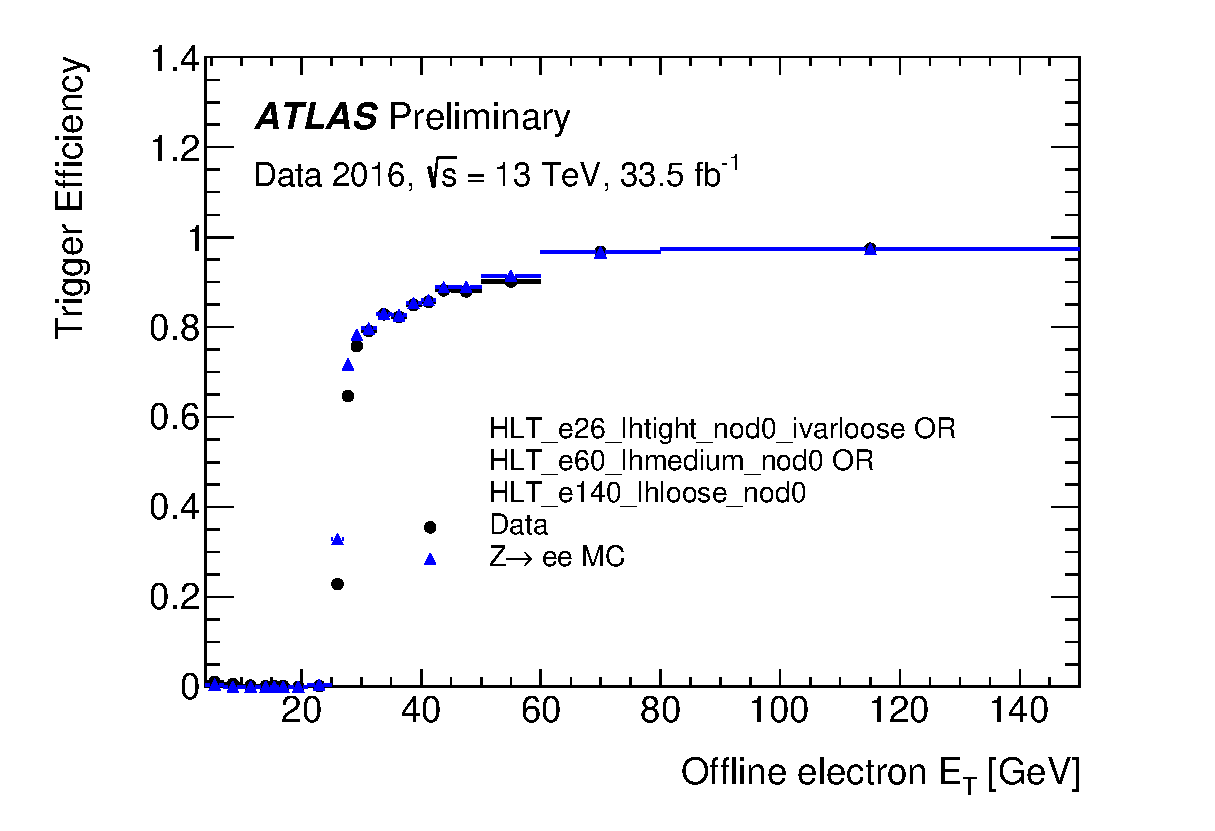
\includegraphics[width=0.55\textwidth]{figures/EventSelection/Eff_Et_singleOR_full2016}
\caption[Electron trigger efficiencies for 2016]{The efficiency of the logical OR between the three un-prescaled electron triggers used in this search~\cite{trig_eff_2016}.}
\label{fig:trig_eff}
\end{figure}

The corresponding lowest $E_{\rm T}$-threshold, un-prescaled, single muon triggers have only a 70\,\% efficiency in the plateau region, due to limited coverage of muon trigger hardware. The $\mu$-channel therefore uses a \MET trigger. At the trigger level, \MET is calculated only using calorimeter energy, ignoring contributions from muons in the MS. Effectively, the \MET measured at trigger level corresponds to the $E_{\rm T}(W\ra\mu\nu)$ measured at reconstruction level.  This trigger has an efficiency of approximately 100\,\% for events with \\$\pT(W\ra\mu\nu)>200\,\GeV$. Contamination from events with multiple muons or no muons can be mitigated by requiring exactly one signal muon. The increased acceptance of the \MET trigger corresponds to a 10\,\% improvement in sensitivity in the combined $e+\mu$ channel. Notably, the gain in efficiency is important in the high mass region, which is particularly sensitive to signal acceptance. 

Since \MET is strongly affected by $\langle\mu\rangle$, the \MET trigger thresholds were raised multiple times to combat the rising trigger rates. In 2015, \MET was calculated using the cell method: \MET is calculated as the negative sum of the $E_{\rm T}$ in all calorimeter cells. Starting in 2016, \MET was calculated using the the missing $H_{\rm T}$ (MHT) algorithm. For MHT, the negative vector sum of the \pT of calibrated anti-$k_{\rm T}$ jets is used to define \MET.

%
\section{Event Preselection}
\label{ch:event_selection:pre}
Before the analysis selection cuts are applied, a preselection is imposed to reject events with detector or reconstruction problems, and to reduce the dataset size. The first stage is called event cleaning, and is standardized for ATLAS physics analyses.

\begin{itemize}
\item\underline{Good Runs List}: A GRL selection is applied to ensure the data corresponds to periods of time (lumi-blocks) where the detector was fully operational, and the data collected was of adequate quality. The LHC beams are required to be stable, the magnets are required to be on (and not ramping), and all subdetectors are required to be on, with not too many noisy cells.
\item\underline{Primary Vertex}: The event is required to have a primary vertex with at least two tracks, each with $p_{\rm T, trk}>400\,\MeV$. If more than one vertex satisfies the requirement, the one with the largest $\sum p_{\rm T, trk}^2$ is selected. 
\item\underline{Subdetector Error Veto}: Corrupted events from the LAr and Tile calorimeters, and the SCT are vetoed. Events are also rejected if they occur close to a noise burst in the LAr calorimeter. 
\item\underline{Incomplete Events}: If for any reason a recorded event is missing detector information, it is rejected.
\end{itemize}

After the event cleaning cuts, the rest of the preselection cuts are applied, where signal and veto leptons are defined in~\Ch{\ref{ch:objreco}}:

\begin{itemize}
	\item\underline{Bad Jet Veto}: Noise bursts or coherent noise in the calorimeters, hardware issues, beam backgrounds, and cosmic muons can create fake jets. A high efficiency working point, called BadLoose, is defined to reject events with ``bad" jets~\cite{bad_jet}. These bad jets can degrade the calculation of \MET. Since electrons and muons can be reconstructed as bad jets, the overlap removal procedure between signal and veto leptons and jets is applied before the bad jet veto.  %\href{https://twiki.cern.ch/twiki/bin/view/AtlasProtected/HowToCleanJets2016}{Veto whole event} if there is a badjet after overlap removal.
    \item\underline{Second Lepton Veto}: The event is required to have exactly one lepton, with no ``veto'' leptons.
 	\item\underline{Signal lepton}: The lepton is required to pass the signal lepton definition.
	\item\underline{Trigger Matching}: The reconstructed signal lepton is required to match the physics object that passed the initial trigger. 
	%\item {$\pt(\ell\nu) > 75\,\GeV$}
	%\item {At least one large-R jet}
\end{itemize}

%
\section{Event Reweighting}
The generated MC samples require various weights in order to ensure their distribution agrees with the distribution observed in data. As mentioned in~\Sect{\ref{ch:analysisStrategy:sig_bkg_model}}, a PU reweighting is applied to MC samples to match the measured PU distribution. Weights are also applied due to the different efficiencies of reconstructed objects from MC and from data. For leptons, weights are applied to correct for reconstruction and isolation efficiencies. Electrons have additional weights for identification, and for trigger and matching efficiencies. Muons have weights applied for the efficiency of associating tracks to a vertex. Jets have weights applied due to efficiencies of $b$-tagging~\cite{b_jet} and the jet vertex tagger. Finally, the MC samples are scaled to the measured integrated luminosity, taking into account higher order corrections to cross sections and filter efficiencies (enforcing a specific final state, e.g. leptonic decay of a top quark).
%$N_{exp} = \sigma \times BR \times \mathcal\times k_{factor}\times \epsilon_{filter}\times{L}_{int}$
% $N_{pred} = N_{gen, pass selection} \times N_{exp} / N_{generated}$

%
\section{Event Categorization by Production Mechanism}
After preselection, events are categorized according to whether they are compatible with VBF production. As motivated in~\Sect{\ref{ch:evt_sel:sig_eff}}, the VBF production region is prioritized.  Events passing the selection criteria are categorized as ``VBF selection'', while, for brevity, events failing the selection criteria are categorized as ``ggF selection'', where the ggF selection is meant to encompass qqF production as well. 
%Moreover, there can be signal leak between categories, but every event will be classified as either a VBF selection or ggF selection.

The VBF selection is summarized in~\Tab{\ref{tab:vbf_sel}}. The selection requires at least two VBF candidate small-R jets, as defined in~\Sect{\ref{ch:objectReconstruction:smallr}}. If there are more than two such jets, the two with the highest invariant mass, $m^{\rm VBF}(j,j)$, are selected. Jets from VBF production are expected to have a small deflection from the beamline, thus, the jets are required to be in different hemispheres of the detector, $\eta(j_1)\cdot\eta(j_2)<0$.  The pair of jets are then required to satisfy, $m^{\rm VBF}(j,j)>770\,\GeV$, and have a separation of $|\Delta\eta^{\rm VBF}(j,j)|>4.7$.  

All events that fail the VBF selection are treated in the ggF selection category. The selection efficiency of VBF jets from signal samples with VBF production is approximately 28\,\%. Only 1\,\% of signal samples produced with ggF (or qqF) pass the VBF selection.
% The mass and separation cuts were chosen to harmonize with $llqq$ channel, and is consistent with the maximum sensitivity region of this analysis.

\begin{table}[htb]
\centering
\begin{tabular}{l|c}
\hline\hline
Selection & Requirement\\\hline
Num. VBF candidate jets &$\geq 2$\\
&(if $>2$, select highest $m^{\rm VBF}(j,j)$ pair)\\
Separate Hemispheres&$\eta(j_1)\cdot \eta(j_2)<0$\\
Invariant Mass [\GeV]&$m^{\rm VBF}(j,j)>770$\\
Separation&$|\Delta\eta^{\rm VBF}(j,j)|>4.7$\\\hline\hline
\end{tabular}
\caption[Vector boson fusion event selection criteria]{Summary of the criteria for the VBF event selection.}
\label{tab:vbf_sel}
\end{table}

%
\section{Kinematic and Topological Selections}
After the event is categorized according to the production mechanism, a series of kinematic and topological cuts are placed in order to select events from the boosted regime. 
\begin{itemize}
\item\underline{Large-R Jet}: At least one large-R jet satisfying the definition in~\Sect{\ref{ch:objectReconstruction:larger}} is required. If more than one exists, the one with the largest $\pT$ is selected. For the VBF event selection, the large-R jet is required to not overlap with the VBF selected jets: $\Delta R(j_1^{\rm VBF},J)>1.5$ and $\Delta R(j_2^{\rm VBF},J)>1.5$.
\item\underline{Multijet Cleaning:} Requiring $\MET>100\,\GeV$\, removes nearly all the multijet background. A further requirement is placed to remove a small number of multijet events which fake a high-\pT electron with an associated low amount of \MET. The $e$-channel is required to satisfy: $\MET/\pT(W\ra e\nu)>0.2$. The multijet background is estimated to be negligible after these cuts, as detailed in~\App{\ref{ch:qcd}}. 
\item\underline{Boosted Regime:} The leptonically decaying boson is required to be sufficiently boosted: $\pT(W\ra\ell\nu)>200\,\GeV$. This also ensures the \MET trigger is fully efficient in the $\mu$-channel.
\item\underline{Relative Boson \pT}: Since the weak bosons from the resonance decay are expected to have \pT equal to approximately half the resonance mass, events are rejected if the ratio of the weak boson \pT to the invariant mass of the $WV\ra\ell\nu J$ system is too low. The optimal cut values were found not to depend on signal mass, and for simplicity, the thresholds for the leptonic and hadronic decays are equal. The VBF threshold is lower to increase signal efficiency. 
\begin{itemize}
\item $\pT(W\ra\ell\nu)/m(WV\ra\ell\nu J) > 0.3\, (0.4)$ for VBF (ggF) selection
\item $\pT(J)/m(WV\ra\ell\nu J) > 0.3\, (0.4)$ for VBF (ggF) selection
\end{itemize}
\end{itemize}



%
\section{Signal and Control Regions}
\label{ch:eventSelection:srcr}
This search is sensitive to both charged and neutral resonances. Two channels exist, corresponding to whether the large-R jet is tagged as a $W$ or $Z$ boson. Since the SmoothedWZTagger uses a mass window to identify the boson, there is a large overlap between the $WW$-channel and the $WZ$-channel. The overlap is acceptable since signal models will only be evaluated in one channel. Both the 50\,\% and 80\,\% efficiency working points of the SmoothedWZTagger are used to define the signal regions (SR) and control regions (CR). A high purity (HP) region is defined in~\Sect{\ref{ch:evt_sel:hp}}, and a low purity (LP) region, meant to recover additional signal events, is defined in~\Sect{\ref{ch:evt_sel:lp}}.

%
\subsection{High Purity Selection}
\label{ch:evt_sel:hp}
The HP selection is designed to have the highest sensitivity to signals in the high mass region, where the SM background is expected to be low. The HP SR is defined by the following selection:
\begin{itemize}
\item\underline{$b$-jet Veto}: Events with a small-R jet tagged as a $b$-jet (\Sect{\ref{ch:objectReconstruction:smallr}}) are vetoed if the $b$-jet lies outside the large-R jet: $\Delta R(J,b)>1.0$. This cut rejects approximately 70\,\% of \ttbar events, while maintaining a signal efficiency of approximately 95\,\%.
\item\underline{Boson Tagging}: The large-R jet is required to pass the 50\,\% efficiency working point for the $W$ or $Z$ boson mass window cut (it is possible for a large-R jet to pass both). Additionally, the large-R jet is required to pass the 50\,\% efficiency working point for the \pT-dependent upper cut on the $D_2^{\beta=1}$ substructure variable. 
\end{itemize}
In~\Fig{\ref{fig:evt_sigbkg_hp}}, shape differences between background and signal MC distributions of the large-R jet mass, $D_2^{\beta=1}$, and relative \pT are shown in the HP SR.

\begin{figure}[tbp]
\centering
\subfloat[]{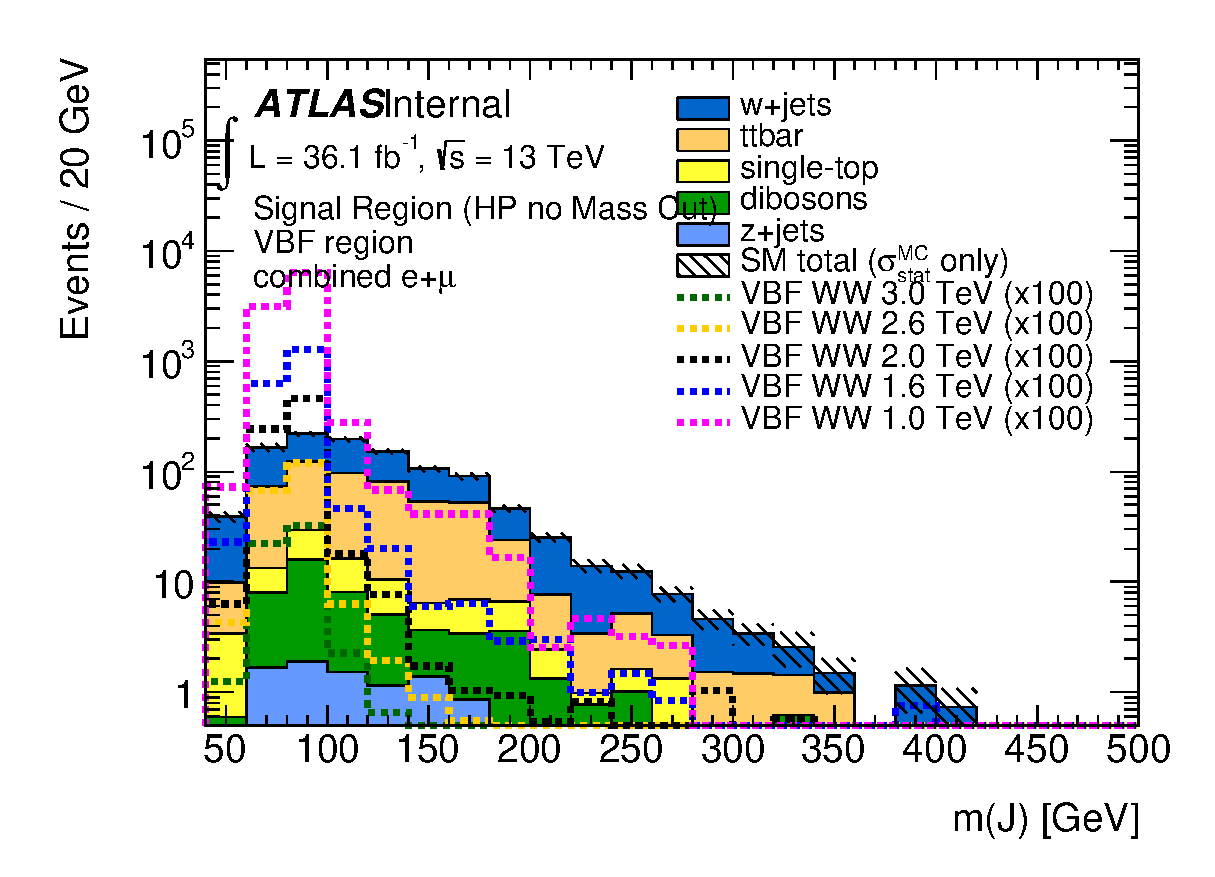
\includegraphics[width=.49\textwidth]{figures/EventSelection/JM_5_comb_VBF}\label{fig:evt_sigbkg_hp:a}}
\subfloat[]{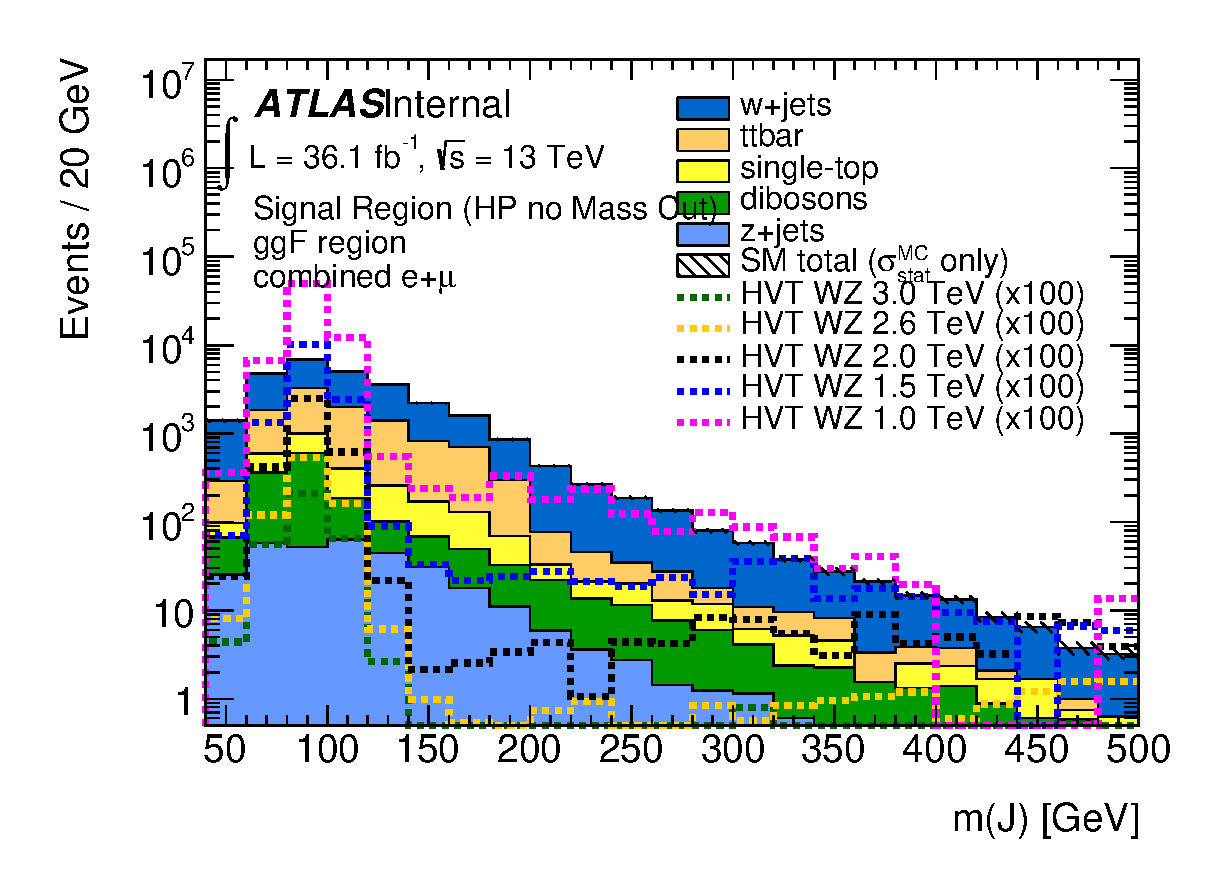
\includegraphics[width=.49\textwidth]{figures/EventSelection/JM_5_comb_ggF}\label{fig:evt_sigbkg_hp:b}}\\
\subfloat[]{\includegraphics[width=.49\textwidth]{figures/EventSelection/JD2_1_comb_VBF}\label{fig:evt_sigbkg_hp:c}}
\subfloat[]{\includegraphics[width=.49\textwidth]{figures/EventSelection/JD2_1_comb_ggF}\label{fig:evt_sigbkg_hp:d}}\\
\subfloat[]{\includegraphics[width=.49\textwidth]{figures/EventSelection/JPt_over_M_6_comb_VBF}\label{fig:evt_sigbkg_hp:e}}
\subfloat[]{\includegraphics[width=.49\textwidth]{figures/EventSelection/JPt_over_M_6_comb_ggF}\label{fig:evt_sigbkg_hp:f}}
\caption[Large-R jet distributions in the high purity signal regions]{Large-R jet mass in the HP SR (without $m(J)$ window cut) for the \protect\subref{fig:evt_sigbkg_hp:a} VBF and \protect\subref{fig:evt_sigbkg_hp:b} ggF selection. Large-R jet $D_2^{\beta=1}$ distribution in the HP SR (without $D_2^{\beta=1}$ upper cut) for the  \protect\subref{fig:evt_sigbkg_hp:c} VBF and \protect\subref{fig:evt_sigbkg_hp:d} ggF selection. Large-R jet relative \pT in the HP SR (without relative \pT cuts) for the \protect\subref{fig:evt_sigbkg_hp:e}VBF selection and \protect\subref{fig:evt_sigbkg_hp:f} ggF selection. Signal samples for masses between 1\,\TeV\, and 3\,\TeV\, are overlaid and scaled to 100 times the cross section. A scalar Higgs (HVT $W'$) model is used for the VBF (ggF) selection. All samples are scaled to 36.1\,\ifb.}
\label{fig:evt_sigbkg_hp}
\end{figure}

In the HP SR, the principal backgrounds are \Wjets and \ttbar, contributing approximately 50\,\% (60\,\%) and 45\,\% (30\,\%), respectively in the VBF (ggF) selection region. Dedicated CRs are defined to estimate the normalizations for both of these backgrounds, and verify accurate modeling. The CRs are crafted to be orthogonal to the SR, yet as kinematically similar as possible. The HP CRs are defined as follows:
\begin{itemize}
\item\underline{\Wjets CR (HP)}: The \Wjets CR is defined in the mass sidebands of the large-R jet. The selection is the same as the HP SR, with the exception of the mass window cut. The large-R jet is required to fail the 80\,\% efficiency working point for both the $W$ and $Z$ mass window. Events falling in the region between the 80\,\% and 50\,\% efficiency working points for the mass window will be recovered in the LP SR defined in~\Sect{\ref{ch:evt_sel:lp}}. \Wjets events comprise approximately 55\,\% (70\,\%) of the background in this region for the VBF (ggF) selection, while the remaining background is mostly from \ttbar.
\item\underline{\ttbar CR (HP)}: The \ttbar CR is defined with the same selection as the HP SR, with the exception of the $b-$jet veto. Events are required to have at least one such $b$-jet. Over 85\,\% of the background in the region is from \ttbar. 
\end{itemize}

In both CRs, the signal contamination is negligible. The normalizations of the \Wjets and \ttbar backgrounds are estimated using a simultaneous fit of the CRs discussed in~\Ch{\ref{ch:stats}}. Although the purity in the $\Wjets$ CR is somewhat poor, the high purity of the \ttbar CR allows an accurate determination of the \Wjets normalization in the simultaneous fit. 

%
\subsection{Low Purity Selection}
\label{ch:evt_sel:lp}
Since the HP SR uses the 50\,\% efficiency working point to identify the large-R jet, a LP SR is defined to recover signal events which do not pass the stringent HP requirements. The LP SR requirements include:
\begin{itemize}
\item\underline{$b$-jet Veto}: The same $b$-jet veto as the HP SR is applied.
\item\underline{Boson Tagging}: The large-R jet is required to fail {\em at least one} of the 50\,\% efficiency working points (i.e. either mass window, $D_2^{\beta=1}$, or both). Additionally, the large-R jet must pass {\em both} of the 80\,\% efficiency working points (i.e. both mass window and $D_2^{\beta=1}$).
\end{itemize}
The background composition in the LP SR for the VBF (ggF) selection is approximately 70\,\% (75\,\%) \Wjets and 25\,\% (20\,\%) \ttbar. LP CRs are defined analogously to the HP CRs:
\begin{itemize}
\item\underline{\Wjets CR (LP)}: A $b$-veto is applied, as in the LP SR; however, the large-R jet must fail the 80\,\% working point for the mass window. The large-R jet is additionally required to fail the 50\,\% working point for $D_2^{\beta=1}$ but pass the 80\,\% working point. Approximately 60\,\% (75\,\%) of the background in this region, for the VBF (ggF) selection is due to \Wjets.
\item\underline{\ttbar CR (LP)}: The selection is the same as the LP SR, with the exception of the $b$-veto, which is inverted. Approximately 85\,\% of the background in this region is due to \ttbar.
\end{itemize}

The approximate background composition in the SRs and CRs is summarized in~\Tab{\ref{tab:evt_sel:bkg_comp}}. In~\App{\ref{ch:eventCutflow}}, the event cut flow is presented for the background and selected signal MC samples, for all SRs and CRs.
In~\Fig{\ref{fig:sig_mvv}}, the invariant mass distribution of the diboson system in the SRs is shown for simulated background and signal MC.  An illustration of the HP SR and LP SR selection for large-R jets is given in~\Fig{\ref{fig:hplp_def}}. The complete SR and CR selections are summarized in~\Tab{\ref{tab:SRdefinitions}}.
\begin{table}[hb]
\centering
\begin{tabular}{l|rr|rr|rr|rr}
\hline\hline
Region&\multicolumn{2}{c|}{\Wjets}&\multicolumn{2}{c|}{Top}&\multicolumn{2}{c|}{Diboson}&\multicolumn{2}{c}{\Zjets}\\
&ggF&VBF&ggF&VBF&ggF&VBF&ggF&VBF\\\hline
SR HP (inclusive)&58.3&48.8&32.8&44.4&7.8&5.8&1.0&0.9\\
Top CR HP &6.7&6.3&92.2&92.1&0.8&1.5&0.2&0.2\\
\Wjets CR HP &68.7&55.4&27.4&40.2&2.5&3.4&1.4&1.0\\\hline
SR LP (inclusive)&74.8&67.7&19.8&26.6&4.0&4.1&1.5&1.7\\
Top CR LP&14.5&12.5&84.1&86.1&1.0&1.0&0.5&0.4\\
\Wjets CR LP&73.8&57.8&22.8&38.4&1.9&2.4&1.4&1.5\\\hline\hline
\end{tabular}
\caption[Background composition in signal regions and control regions]{The background composition percentage for each background in the signal regions and control regions. The Top background includes both \ttbar and \Singlet. The inclusive signal regions (SR) includes events from $WW$ or $WZ$ SR. }
\label{tab:evt_sel:bkg_comp}
\end{table}

% Bkg Comp
\begin{figure}[tbp]
\centering
\subfloat[]{\includegraphics[width=.49\textwidth]{figures/EventSelection/VVM_0_comb_VBF}\label{fig:sig_mvv:a}}
\subfloat[]{\includegraphics[width=.49\textwidth]{figures/EventSelection/VVM_0_comb_ggF}\label{fig:sig_mvv:b}}\\
\subfloat[]{\includegraphics[width=.49\textwidth]{figures/EventSelection/VVM_11_comb_VBF}\label{fig:sig_mvv:c}}
\subfloat[]{\includegraphics[width=.49\textwidth]{figures/EventSelection/VVM_11_comb_ggF}\label{fig:sig_mvv:d}}
\caption[Invariant mass distribution of signal and background samples in the signal regions]{The distribution of $m(WV\ra\ell\nu J)$ for simulated background and signal MC events, in the HP SR for \protect\subref{fig:sig_mvv:a} VBF selection and \protect\subref{fig:sig_mvv:b} ggF selection; and in the LP SR for \protect\subref{fig:sig_mvv:c} VBF selection and \protect\subref{fig:sig_mvv:d} ggF selection. Signal samples for masses between 1\,\TeV\, and 3\,\TeV\, are overlaid and scaled to 100 times the cross section. A scalar Higgs (HVT $W'$) model is used for the VBF (ggF) selection. All samples are scaled to an integrated luminosity of 36.1\,\ifb.}
\label{fig:sig_mvv}
\end{figure}

\begin{figure}[t]
\centering
\caption[Illustration of high purity and low purity signal region for large-R jets]{Illustration of $WW$ (shaded) and $WZ$ (dashed) HP and LP SRs for large-R jets. The SmoothedWZTagger 50\,\% and 80\,\% efficiency $V$-tagging working points define the HP (red) and LP (purple) regions. The value of the $D_2^{\beta=1}$ and mass window cuts depend on $\pt(J)$. The LP SR excludes the HP SR to ensure orthogonality. The $W+$jets CR is defined by the SR mass sidebands (orthogonal to both $WW$ and $WZ$ SR).}
\includegraphics[width=.75\textwidth]{figures/EventSelection/HPLPdefinition}
\label{fig:hplp_def}
\end{figure}
\begin{table}[b]
\centering
\begin{tabular}{l|l|c|c|c}
\hline\hline
\multicolumn{2}{l|}{Selection: HP (LP)} &SR&$W$ CR&\ttbar CR\\ \hline
Production& VBF & \multicolumn{3}{c}{ $m^{\textrm{VBF}}(j,j)>770\,\GeV$ and $|\Delta\eta^{\textrm{VBF}}(j,j)|>4.7$} \\ \cline{2-5}
Category& ggF & \multicolumn{3}{c}{Fail VBF selection} \\ \hline
&\vphantom{\Large B} Signal leptons & \multicolumn{3}{c}{ $1$} \\\cline{2-5}
&\vphantom{\Large B} Veto leptons & \multicolumn{3}{c}{ $0$} \\\cline{2-5}
$W\rightarrow \ell\nu$&\vphantom{\Large B} \met [\GeV]& \multicolumn{3}{c}{ $>100$ } \\ \cline{2-5}
%&\vphantom{\Large B} $\pt(\ell\nu)$ [\GeV]& \multicolumn{3}{c}{ $>200$ } \\ \cline{2-5}
&\vphantom{\Large B} $\met/\pt(e\nu) $ & \multicolumn{3}{c}{ $ > 0.2$ } \\\cline{2-5} 
&\vphantom{\Large B} $\pt(\ell\nu)$ [\GeV]& \multicolumn{3}{c}{ $>200$} \\\hline
&\vphantom{\Large B} Large-$R$ jets & \multicolumn{3}{c}{ $\geq 1$ } \\ \cline{2-5}
&\vphantom{\Large B} $D^{(\beta=1)}_2$ 50\,\% WP &pass (fail$\dagger$)&pass (fail)&pass (fail$\dagger$)\\ \cline{2-5}
$W/Z\rightarrow J$&\vphantom{\Large B} $D^{(\beta=1)}_2$ 80\,\% WP &--- (pass)&--- (pass)&--- (pass)\\ \cline{2-5}
&\vphantom{\Large B} $W/Z$ mass 50\,\% WP &pass (fail$\dagger$)&---  (---)&pass (fail$\dagger$)\\ \cline{2-5}
&\vphantom{\Large B} $W/Z$ mass 80\,\% WP &--- (pass)&fail (fail)&--- (pass)\\ \hline
Topology&\vphantom{\Large B} $\pt(\ell\nu) / m(WV)$ & \multicolumn{3}{c}{ $>0.3$ for VBF and $> 0.4$ for ggF selection}\\\cline{2-5}
Cuts&\vphantom{\Large B} $\pt(J) / m(WV)$ & \multicolumn{3}{c}{$>0.3$ for VBF and $> 0.4$ for ggF selection} \\ \hline
Num. $b$-jets&\vphantom{\Large B} $\Delta R(J,b)>1.0$ & \multicolumn{2}{c|}{0} &$\geq 1$ \\ \hline\hline
\end{tabular}
\caption[Event selection criteria]{Summary of the selection criteria used to define the SR, $W$+jets CR and \ttbar CR, for the HP and LP selections. The LP selections are listed in parentheses. Events are categorized according to their production mechanism where the VBF selection is prioritized.\\ $\dagger$ For the LP SR and LP \ttbar CR, the large-R jet can fail either the 50\,\% efficiency $D_2^{\beta=1}$ working point or the 50\,\% efficiency mass window working point. } 
\label{tab:SRdefinitions}
\end{table}
%\end{figure}

%
\clearpage
\section{Signal Efficiency and Acceptance}
\label{ch:evt_sel:sig_eff}
Signal efficiency times acceptance ($\epsilon\times A$) is defined as the ratio of the number of reconstructed signal events passing the signal region selection, to the total number of generated signal events. In~\Fig{\ref{fig:sig_acc_vbf}} and~\Fig{\ref{fig:sig_acc_ggf}}, $\epsilon\times A$ is plotted as a function of $m(WV\ra\ell\nu J)$ for all signal models with VBF production and ggF (or qqF) production, respectively. \Fig{\ref{fig:sig_acc_vbf}} shows that, for signal models with VBF production, a substantial fraction of signal events leak into the ggF selection category, and the overall $\epsilon\times A$ is smaller than for samples with ggF (or qqF) production. Less than 1\,\% of signals produced by ggF (or qqF) leak into the VBF selection category. Due to these factors, and the smaller cross section for models with VBF production, the VBF selection is prioritized over the ggF selection to increase the sensitivity of the search.

The search is most efficient for higher resonance masses, with most signal models reaching a plateau in $\epsilon\times A$ for $m(WV)>1\,\TeV$. For the models with ggF (or qqF) production, the plateau region corresponds to a total $\epsilon\times A$ between approximately 30\,\% and 35\,\%. The scalar heavy Higgs samples notably have a smaller total $\epsilon\times A$, approximately 20\,\% to 23\,\%. 
In models of higher spin resonances, the two weak bosons are preferentially produced in the central barrel region, while in the scalar resonance model, the production angle of the two weak bosons is uniformly distributed.
%The distribution of the two weak bosons is more peaked in the central barrel region for higher spin resonances than in scalar resonance models. 
Thus, the cuts on $\pT(V)/m(WV)$ reject more signal events for the scalar resonance model than for higher spin resonance models, since a larger fraction of the daughter weak bosons will be produced at larger $|\eta|$, with correspondingly lower \pT, in the scalar model. For most mass points, there is approximately a 50\,\% increase in $\epsilon\times A$ by including the LP SR in addition to the HP SR.

\begin{figure}[tbp]
\centering
\subfloat[]{\includegraphics[width=.49\textwidth]{figures/EventSelection/VBF-HVTWW_effacc}\label{fig:sig_acc_vbf:a}}
\subfloat[]{\includegraphics[width=.49\textwidth]{figures/EventSelection/VBF-HVTWZ_effacc}\label{fig:sig_acc_vbf:b}}\\
\subfloat[]{\includegraphics[width=.49\textwidth]{figures/EventSelection/VBFWWNWA_effacc}\label{fig:sig_acc_vbf:c}}
\caption[Signal efficiency times acceptance for models with vector boson fusion production]{Signal efficiency times acceptance ($\epsilon\times A$) is plotted as a function of $m(WV\ra\ell\nu J)$ for models with VBF production in the high purity (blue) and low purity (red) VBF selection (hollow) and ggF selection (filled) categories, as well as the total combined $\epsilon\times A$ (black star). The signal models include \protect\subref{fig:sig_acc_vbf:a} an HVT $Z'$, \protect\subref{fig:sig_acc_vbf:b} an HVT $W'$, and \protect\subref{fig:sig_acc_vbf:c} a scalar heavy Higgs (NWA). $\epsilon\times A$ is defined as the ratio of the number of signal events reconstructed in the signal region, to the total number of generated signal events. }
\label{fig:sig_acc_vbf}
\end{figure}

\begin{figure}[tbp]
\centering
\subfloat[]{\includegraphics[width=.49\textwidth]{figures/EventSelection/HVTWW_effacc}\label{fig:sig_acc_ggf:a}}
\subfloat[]{\includegraphics[width=.49\textwidth]{figures/EventSelection/HVTWZ_effacc}\label{fig:sig_acc_ggf:b}}\\
\subfloat[]{\includegraphics[width=.49\textwidth]{figures/EventSelection/RSGWW_effacc}\label{fig:sig_acc_ggf:c}}
\subfloat[]{\includegraphics[width=.49\textwidth]{figures/EventSelection/ggHWWNWA_effacc}\label{fig:sig_acc_ggf:d}}
\caption[Signal efficiency times acceptance for models with gluon gluon fusion production]{Signal efficiency times acceptance ($\epsilon\times A$) is plotted as a function of $m(WV\ra\ell\nu J)$ for models with ggF (or qqF) production in the high purity (blue) and low purity (red) ggF selection categories, as well as the total combined $\epsilon\times A$ (black star). The signal models include \protect\subref{fig:sig_acc_ggf:a} an HVT $Z'$, \protect\subref{fig:sig_acc_ggf:b} an HVT $W'$, \protect\subref{fig:sig_acc_ggf:c} a bulk RS Graviton ($k/\overline{M}_{\textrm Pl}=1.0$), and \protect\subref{fig:sig_acc_ggf:d} a scalar heavy Higgs (NWA). $\epsilon\times A$ is defined as the ratio of the number of signal events reconstructed in the signal region, to the total number of generated signal events.}
\label{fig:sig_acc_ggf}
\end{figure}

%
\clearpage
\section{Background Validation}
To validate the background modeling in the control regions, recorded data is overlaid with the background predicted using MC samples. The $m(\ell\nu J)$ distribution is shown in the HP CRs in~\Fig{\ref{fig:datamc_hpcr}}, and in the LP CRs in~\Fig{\ref{fig:datamc_lpcr}}. The ratio of the data to the MC prediction is included, with MC statistical uncertainties overlaid. 

In most regions, the agreement is fairly good, with no noticeable slopes in the ratio plot. The MC samples in the \Wjets CRs predict a higher event yield than is observed. However, the overall normalization will be determined by the fit in~\Ch{\ref{ch:stats}}, and therefore it is only important to examine the agreement in the slopes of the distributions. The CRs for the VBF selection in general show a larger normalization discrepancy between data and MC prediction, with respect to the ggF selection. This behavior has been observed in other similar analyses at ATLAS, and is not an issue in this search because separate normalizations will be determined for the ggF and VBF selections. Distributions for all major kinematic variables related to the event selection were checked, and a similar level of agreement was observed. After the fit, systematic uncertainties (\Ch{\ref{ch:syst}}) will be included in the uncertainty bands, representing a more conservative total estimated uncertainty. 

\begin{figure}[htbp]
\centering
\subfloat[]{\includegraphics[width=.48\textwidth]{figures/BackgroundValidation/VVM_3_comb_VBF}\label{fig:datamc_hpcr:a}}
\subfloat[]{\includegraphics[width=.48\textwidth]{figures/BackgroundValidation/VVM_3_comb_ggF}\label{fig:datamc_hpcr:b}}\\
\subfloat[]{\includegraphics[width=.48\textwidth]{figures/BackgroundValidation/VVM_2_comb_VBF}\label{fig:datamc_hpcr:c}}
\subfloat[]{\includegraphics[width=.48\textwidth]{figures/BackgroundValidation/VVM_2_comb_ggF}\label{fig:datamc_hpcr:d}}
\caption[Data and Monte Carlo comparison in the high purity control regions]{The distribution of $m(\ell\nu J)$ for data from 2015+2016 (36.1\,\ifb) and for the background MC prediction. The VBF selection HP \protect\subref{fig:datamc_hpcr:a} \Wjets CR and \protect\subref{fig:datamc_hpcr:c} \ttbar CR, and the ggF selection HP \protect\subref{fig:datamc_hpcr:b} \Wjets CR and \protect\subref{fig:datamc_hpcr:d} \ttbar CR, are shown. The simulated MC backgrounds are normalized to the recorded luminosity. In the bottom panel, the ratio of the observed data to MC prediction is plotted, with the MC statistical uncertainty overlaid as the shaded band. }
\label{fig:datamc_hpcr}
\end{figure}

\begin{figure}[htbp]
\centering
\subfloat[]{\includegraphics[width=.48\textwidth]{figures/BackgroundValidation/VVM_12_comb_VBF}\label{fig:datamc_lpcr:a}}
\subfloat[]{\includegraphics[width=.48\textwidth]{figures/BackgroundValidation/VVM_12_comb_ggF}\label{fig:datamc_lpcr:b}}\\
\subfloat[]{\includegraphics[width=.48\textwidth]{figures/BackgroundValidation/VVM_13_comb_VBF}\label{fig:datamc_lpcr:c}}
\subfloat[]{\includegraphics[width=.48\textwidth]{figures/BackgroundValidation/VVM_13_comb_ggF}\label{fig:datamc_lpcr:d}}
\caption[Data and Monte Carlo comparison in the low purity control regions]{The distribution of $m(\ell\nu J)$ for data from 2015+2016 (36.1\,\ifb) and for background MC prediction. The VBF selection LP \protect\subref{fig:datamc_lpcr:a} \Wjets CR and \protect\subref{fig:datamc_lpcr:c} \ttbar CR, and ggF selection LP \protect\subref{fig:datamc_lpcr:b} \Wjets CR and \protect\subref{fig:datamc_lpcr:d} \ttbar CR, are shown. The simulated MC backgrounds are normalized to the recorded luminosity. In the bottom panel, the ratio of the observed data to MC prediction is plotted, with the MC statistical uncertainty overlaid as the shaded band.}
\label{fig:datamc_lpcr}
\end{figure}








%%________________
%% DATA:
%% Background Validation
%% Systematics
%% Results
%%----------------
% !TEX root = ../main.tex
%%__________________________________
%% 
%% Systematics, Statistical Analysis,
%% Results
%%----------------------------------


% !TEX root = ../../main.tex
\chapter{Systematic Uncertainties} 
\label{ch:syst}

In this chapter, the systematic uncertainties considered in this analysis are specified. In \Sect{\ref{ch:syst:exp_unc}}, experimental uncertainties related to physics objects are described. \Sect{\ref{ch:syst:bkg_unc}} outlines the systematic uncertainties related to background modeling.  In \Sect{\ref{ch:syst:sig_unc}}, the theoretical uncertainties related to signal modeling are explained. In the statistical analysis described in~\Ch{\ref{ch:stats}}, each systematic uncertainty is treated as a nuisance parameter (NP). Event yields for the background and signal samples are determined corresponding to varying the systematic uncertainties by $\pm 1\sigma$.

%%
\section{Experimental Uncertainties}
\label{ch:syst:exp_unc}
Experimental uncertainties related to reconstructed physics objects are considered.  These uncertainties can affect both the shape and the normalization of simulated background and signal distributions. 

%
\subsection{General Uncertainties}
The total integrated luminosity for the 2015 + 2016 dataset used in this analysis has a 3.2\,\% uncertainty, measured following the prescription in~\Ref{\cite{lumi_unc}}. A calibration of the luminosity scale was performed in August 2015 and May 2016 with $x-y$ beam separation scans. This uncertainty is applied to the scaled event yields of all generated MC samples.

Variation in the PU re-weighting of MC is included to cover the uncertainty on the ratio between the predicted and measured inelastic cross section in the fiducial volume defined by $M_X>13\, \GeV$, where $M_X$ is the mass of the hadronic system~\cite{prw_unc}. The variation in re-weighting is applied to all generated MC samples. 

%
\subsection{Leptons}
Uncertainties for reconstructed leptons have a minor impact on this analysis. Uncertainties are considered for trigger efficiencies, reconstruction and identification efficiencies, isolation efficiencies, and determination of the momentum scale and resolution~\cite{electron_efficiency_2016, muon_eff}. For muons, the uncertainty on the \MET trigger efficiency is considered, including efficiency differences between \ttbar and \Wjets MC samples. The rest of the uncertainties are estimated using data and MC samples corresponding to $Z\ra \ell^+\ell-$ and $J/\Psi\ra\ell^+\ell^-$ resonances, with a tag and probe method where isolated leptons are used to tag the event. The estimated uncertainties depend on both $\eta$ and $\pT$. They are propagated and applied to the scale factors used to correct the simulated MC samples. The uncertainty on the electron (muon) reconstruction and identification efficiencies is $<0.5\,\%$ ($<1.0\,\%$). For muons, this includes an uncertainty corresponding to the efficiency of the track to vertex association. For both types of leptons, the isolation efficiency has an associated uncertainty below $1\,\%$. The momentum scale and momentum resolution have approximate uncertainties of $0.5\,\%$ ($0.05\,\%$) and $1\,\%$ ($2\,\%$) for electrons (muons), respectively. The uncertainty applied to the muon momentum scale includes charge-dependent effects.  

%
\subsection{Small-R Jets}

For small-R jets, uncertainties are included to account for the efficiency of the jet vertex tagger (JVT), the jet energy scale and resolution (JES, JER) calibrations, and $b$-tagging efficiencies. To account for the JVT efficiencies, an uncertainty of approximately 1\,\% is propagated to the scale factor applied to MC samples. 

The dominant systematic uncertainty for small-R jets is the uncertainty on the JES. Over 80 nuisance parameters (NP) are combined into a ``globally reduced'' set of 21 parameters that depend on $\eta$ and $\pT$~\cite{jes_unc}. There are eight {\em in situ} NPs related to the \pT balance between jets and reference objects ($Z$ boson, photon, multijets) and their response in data and MC. The remaining NPs are MC-based and cover effects including eta inter-calibration, PU, and jet flavor. The total JES uncertainty is presented in~\Fig{\ref{fig:jes_unc}}. For central jets, the relative uncertainty ranges from approximately $6\,\%$ for jets with $\pT=25\,\GeV$\, to 1\,\% for jets with $\pt=1\,\TeV$. The energy resolution of the small-R jet has an associated uncertainty ranging from approximately $10-20\,\%$ for jets with $\pT=20\,\GeV$\, to less than $5\,\%$ for jets with $\pT>200\,\GeV$. 

\begin{figure}[tb]
\centering
\subfloat[]{\includegraphics[width=.48\textwidth]{figures/SystematicUncertainties/jes_unc}\label{fig:jes_unc:a}}
\subfloat[]{\includegraphics[width=.48\textwidth]{figures/SystematicUncertainties/jes_eta}\label{fig:jes_unc:b}}
\caption[Fractional jet energy scale uncertainty for small-R jets]{The fractional jet energy scale uncertainty for central small-R jets, as a function of \protect\subref{fig:jes_unc:a} \pt (with $\eta=0$) and \protect\subref{fig:jes_unc:b} $\eta$\, (for $\pT=60\,\GeV$)~\cite{jes_unc}.}
\label{fig:jes_unc}
\end{figure}

Uncertainties on $b$-tagging efficiency and misidentification rates for small-R jets are considered~\cite{b_jet, b_jet_opt}. The uncertainties are propagated to the scale factors applied to MC samples using a reduced set of 14 NPs, called the ``medium'' prescription. There are three, four, and five NPs considered for the tagging efficiency of jets from $b$-hadrons, $c$-hadrons, and light flavor quarks, respectively. Additional NPs account for jets with $\pT$ values above the kinematic reach of the calibration sample, and for extrapolating $c$-jet scale factors to \tau-induced jets. % About 5-10\% uncertainty for b-tag jets

%
\subsection{Large-R Jets}
\label{ch:syst:largerjets}
Uncertainties related to the scale of large-R jet $\pT$, mass, and $D_2^{\beta=1}$ are considered~\cite{J_scale_unc}. Several recommended configurations are provided; however, the choice was determined to have a negligible impact on this study. For consistency with similar searches, the ``medium'' configuration is used.  In this prescription, the $\pT$ and mass scale uncertainties are fully correlated, while the $D_2^{\beta=1}$ scale uncertainty is left independent.  Four NPs are considered for both the substructure, and kinematic scale uncertainties (eight total). These account for differences between data and MC, modeling differences between MC generators, tracking uncertainties, and statistical uncertainties. The uncertainties are estimated using the ratio of calorimeter-based to track-assisted-based variables in data and MC. The ratios are evaluated at both the calorimeter jet mass scale, and the track-assisted jet mass scale. The large-R jet scale uncertainties range from approximately $2-5\,\%$, as shown in~\Fig{\ref{fig:J_unc}}.

\begin{figure}[tb]
\centering
\subfloat[]{\includegraphics[width=.48\textwidth]{figures/SystematicUncertainties/J_comb_scale}\label{fig:J_unc:a}}
\subfloat[]{\includegraphics[width=.48\textwidth]{figures/SystematicUncertainties/J_d2_scale}\label{fig:J_unc:b}}
\caption[Fractional scale uncertainty for large-R jet \pT, mass, and $D_2^{\beta=1}$]{The fractional scale uncertainty for large-R jet \protect\subref{fig:J_unc:a} combined mass and \protect\subref{fig:J_unc:b} $D_2^{\beta=1}$, as a function of  \pt. Plots are updated from the procedure used in~\Ref{\cite{jet_comb_mass}}.}
\label{fig:J_unc}
\end{figure}


Resolution uncertainties are applied for large-R jet $\pT$, mass, and $D_2^{\beta=1}$. The recommended procedure is to apply a 2\,\% absolute uncertainty for \pT resolution, and a 20\,\% (15\,\%) relative uncertainty for mass resolution ($D_2^{\beta=1}$ resolution). The absolute uncertainty is applied by smearing the large-R jet \pT with a Gaussian of width, $\sigma=\pT\times2\,\%$. 

The relative uncertainties are applied such that the reconstructed mass ($D_2^{\beta=1}$) has an increased resolution of 20\,\% (15\,\%). First, the MC response of the variable (ratio of reconstructed to truth value) is fit with a Gaussian to extract the width, which gives an estimate of the nominal resolution, $\sigma_{\rm nom}$. The nominal resolution is then smeared with a Gaussian of width $0.66\times\sigma_{\rm nom}$ ($0.57\times\sigma_{\rm nom}$) to increase the measured resolution by 20\,\% (15\,\%)\footnote{
	To increase the resolution by 20\,\%, $(1.2\sigma_{\rm nom})^2 = \sigma_{\rm nom}^2 + (f_{\rm smear}\sigma_{\rm nom})^2$. This corresponds to $f_{\rm smear}=0.66$.
}. The $D_2^{\beta=1}$ response distribution is not approximated well by a Gaussian fit, thus the inter-quartile range is used to estimate the nominal resolution. To be conservative, an additional 2\,\% is added to the smearing value for both the mass and $D_2^{\beta=1}$ resolution. In~\Fig{\ref{fig:larger_res}}, the measured mass and $D_2^{\beta=1}$ resolutions are presented as a function of $\pT$. The $\eta$ dependence, and the difference in resolutions between $W$ and $Z$ jets, were determined to be negligible. Therefore, the smearing is applied only as a function of $\pT$.

\begin{figure}[htb]
\centering
\subfloat[]{\includegraphics[width=.48\textwidth]{figures/SystematicUncertainties/mass_resolution}\label{fig:larger_res:a}}
\subfloat[]{\includegraphics[width=.48\textwidth]{figures/SystematicUncertainties/d2_resolution}\label{fig:larger_res:b}}
\caption[Large-R jet mass and substructure resolution]{The measured large-R jet \protect\subref{fig:larger_res:a} mass resolution and \protect\subref{fig:larger_res:b} $D_2^{\beta=1}$ resolution. The mass resolution is measured separately for high purity and low purity large-R jets. The $D_2^{\beta=1}$ resolution is estimated with the interquartile range (instead of a gaussian fit), resulting in a very conservative uncertainty.}
\label{fig:larger_res}
\end{figure}


%
\subsection{Missing Transverse Energy}
The systematic uncertainties associated with all the reconstructed objects used to build the event \MET are propagated to the reconstructed \MET object, and taken as fully correlated to the uncertainties of the constituent objects. This is the main source of \MET uncertainty. Additional uncertainties are calculated to cover the soft terms in the reconstructed \MET, which involve tracks that are unassociated with any reconstructed object. An uncertainty of approximately 2\,\% is included to cover variations in resolution and scale of the soft term~\cite{met_syst}.


%%
\section{Background Uncertainties}
\label{ch:syst:bkg_unc}
Several systematic uncertainties are included to account for uncertainties in the modeling of the simulated backgrounds. For the two main backgrounds in this search, \Wjets and \ttbar, the normalizations are free to float in the fit (\Ch{\ref{ch:stats}}), and systematics uncertainties are estimated to account for the shape of the $m(\ell\nu J)$ distribution in the SRs.

Both the \Singlet and \Zjets backgrounds contribute a small amount to the total estimated SM background in this search. The shapes for these backgrounds are derived exclusively from the MC prediction. A systematic uncertainty is applied to the normalizations of the \Singlet and \Zjets backgrounds to account for the uncertainty in the SM cross section measurement. The normalizations are allowed to float, with an imposed Gaussian constraint with 11\,\% width.

The SM diboson production cross section is fixed to the inclusive NLO calculation. A systematic uncertainty on the normalization is applied in the same manner as for the \Singlet and \Zjets backgrounds. In this case, the width of the Gaussian constraint is set to 30\,\%, in order to cover both the production cross section uncertainty ($\sim11\,\%$) and the factorization and renormalization scale uncertainty ($\sim20\,\%$). Alternative samples produced with \textsc{Powheg-Box+Pythia} are compared to the nominal \textsc{Sherpa} samples, and used to evaluate any shape modeling uncertainty. The shape difference of the invariant mass distribution between the two MC generators was determined to be negligible. 

%
\subsection{\Wjets Shape Uncertainties}
% Factorization scale: separate hard from soft QCD processes (pert. vs non-pert)
% Renorm scale: Energy scale where you set mu when you renormalize, i.e. top mass etc
% Resummation scale: deal with gluon radiation (otherwise diverges) done at leading log (LL)

Following the recommended procedure, the following modeling variations are considered to estimate the uncertainty in the shape of the \Wjets background:
\begin{itemize}
\item Factorization and renormalization scale variations
\item PDF variations
\item $\alpha_s$ variations
\item CKKW matching scale variations~\cite{ckkw} (for $2\ra n$ processes, how to combine matrix element calculations with parton showering calculations without double counting)
\item Resummation scale variations
\end{itemize}
The corresponding parameters are varied in the nominal generator, \textsc{Sherpa}, to estimate the uncertainty. Additionally, alternative samples generated with \textsc{MadGraph} are compared to the nominal \textsc{Sherpa} samples to estimate systematic uncertainties related to parton showering and matrix element implementations.

For each systematic variation, the normalization is fixed such that the event yield in the \Wjets CR is equal to that of the nominal sample. In each SR, the ratio between the variation and nominal $m(\ell\nu J)$ distribution is calculated on a bin-by-bin basis. A linear fit is applied to the ratio in each SR in order to characterize the uncertainty on the shape modeling from the variation. In~\Fig{\ref{fig:wj_syst}}, the HP \Wjets CR is shown for both the VBF and ggF selection, with the dominant systematic shape uncertainties overlaid.

\begin{figure}[htb]
\centering
\subfloat[]{\includegraphics[width=.49\textwidth]{figures/SystematicUncertainties/VVM_CRWHP_ggF}\label{fig:wj_syst:a}}
\subfloat[]{\includegraphics[width=.49\textwidth]{figures/SystematicUncertainties/VVM_CRWHP_VBF}\label{fig:wj_syst:b}}
\caption[\Wjets modeling variations in the \Wjets high purity control region]{The $m(\ell\nu J)$ distribution in the \Wjets CR for \protect\subref{fig:wj_syst:a} ggF selection and \protect\subref{fig:wj_syst:b} VBF selection. Dominant \Wjets modeling uncertainties affecting the shape are shown by colored lines: factorization and renormalization scale variation (red), $\alpha_s$ variation (violet), PDF variation (blue) and \textsc{Sherpa}/\textsc{MadGraph} difference (cyan). The normalization is allowed to float in the final fit described in~\Ch{\ref{ch:stats}}.}
\label{fig:wj_syst}
\end{figure}

%
\subsection{\ttbar Shape Uncertainties}
To estimate the shape uncertainty of the $m(\ell\nu J)$ distribution for the \ttbar background, alternative samples generated with \textsc{MC@NLO} are compared to the nominal samples generated with \textsc{Powheg-Box}. Additional uncertainties related to parton showering are estimated by comparing alternative samples using \textsc{Herwig++} to the nominal samples using \textsc{Pythia}. Renormalization and factorization scale uncertainties are estimated by setting the corresponding parameters in the nominal generator to one half, and to double their nominal values. 

Analogous to the \Wjets procedure, the normalization of the systematic variations are fixed such that the event yield in the \ttbar CR is equal to that of the nominal sample. For each SR, the ratio between the variation and the nominal $m(\ell\nu J)$ distribution is calculated bin-by-bin. Finally, a linear fit is applied to the ratio to estimate the uncertainty on the shape modeling from the variation. 


%%
\section{Signal Uncertainties}
\label{ch:syst:sig_unc}
The largest contributions to the uncertainty on the event yield of the generated signal samples are from initial state and final state radiation (ISR and FSR, respectively), and choice of PDF. 

%
\subsection{Initial State and Final State Radiation Uncertainties}
Following the prescription in~\Ref{\cite{pythia_tune}}, five variations are considered to account for ISR and FSR uncertainties. The variations account for uncertainties related to the underlying event (one), jet substructure (one), and aspects of extra jet production (three). The variations are summed in quadrature and compared to the nominal distribution to estimate the uncertainty. A fourth-order polynomial is fit to the uncertainties, as shown in~\Fig{\ref{fig:isrfsr}}. For most signal models, the estimated uncertainty is approximately 4\,\%.

%
\subsection{Parton Distribution Function Uncertainties}
The uncertainty on the event yield due to choice of PDF is evaluated by comparing samples with the nominal PDF choice, \textsc{NNPDF3.0}, to alternative samples generated with \textsc{MMHT2014}~\cite{mmht} and \textsc{CT14}~\cite{CT14} PDFs\footnote{
	The nominal RS $G^*$ samples are generated with the \textsc{CT14} PDF set, thus the uncertainty is estimated with alternative samples using the \textsc{NNPDF3.0} and \textsc{MMHT2014} PDF sets.
}. Following the prescription in~\Ref{\cite{pdf_env}}, the 68\,\% uncertainty bands for each PDF set are used to evaluate the variations, and the envelope of the three variations is kept to estimate the signal uncertainty. The uncertainty is measured on the ratio of the efficiency times acceptance ($\epsilon\times A$) of the variation samples to the nominal samples. In~\Fig{\ref{fig:pdf}}, the estimated uncertainty due to choice of PDF is shown for the HVT $Z'$ signal model. The estimated uncertainties range among the signal models from approximately $0.5-2.0\,\%$.
\begin{figure}[tb]
\centering
\subfloat[]{\includegraphics[width=.49\textwidth]{figures/SystematicUncertainties/ISRFSR_HVT3}\label{fig:isrfsr:a}}
\subfloat[]{\includegraphics[width=.49\textwidth]{figures/SystematicUncertainties/ISRFSR_RSG3}\label{fig:isrfsr:b}}
\caption[Initial state and final state radiation uncertainties]{Estimated uncertainties related to ISR and FSR in the HP SR for \protect\subref{fig:isrfsr:a} the HVT $W'$ signal model and \protect\subref{fig:isrfsr:b} the RS $G^*$ signal model.}
\label{fig:isrfsr}

\end{figure}
\begin{figure}[htb]
\centering
\subfloat[]{\includegraphics[width=.49\textwidth]{figures/SystematicUncertainties/pdfUncertaintyTotal_HVTWW}\label{fig:pdf:a}}
\subfloat[]{\includegraphics[width=.49\textwidth]{figures/SystematicUncertainties/pdfUncertaintyTotal_HVTWWVBF}\label{fig:pdf:b}}
\caption[Parton distribution function uncertainties]{The estimated PDF uncertainty from \textsc{NNPDF3.0} (black), \textsc{MMHT} (blue), and \textsc{CT14} (red) on the relative signal acceptance for the HVT $Z'$ signal model with \protect\subref{fig:pdf:a} ggF production and \protect\subref{fig:pdf:b} VBF production. The envelope of these variations is chosen as the signal uncertainty.}
\label{fig:pdf}
\end{figure}


% !TEX root = ../../main.tex
\chapter{Statistical Analysis}
\label{ch:stats}

In this chapter, the quantitative strategy used to compare the recorded data to SM predictions, and to set limits on BSM theoretical models, is outlined. The invariant mass distribution, $m(\ell\nu J)$, is used as a discriminant in this search, with an optimized binning strategy as detailed in~\Sect{\ref{ch:stats:vb}}. In \Sect{\ref{ch:stats:ml}}, a maximum-likelihood (ML) fit of the data to a background-only hypothesis, to determine the normalizations of the \Wjets and \ttbar backgrounds, is described. The systematic uncertainties described in~\Ch{\ref{ch:syst}} are included in the fit as nuisance parameters (NP), and the SRs and CRs are fit simultaneously. In \Sect{\ref{ch:stats:ul}}, a test statistic based on the profiled log likelihood ratio, used to create upper limits on production cross sections, is outlined. 

%
\section{Variable Binning}
\label{ch:stats:vb}
In the ML fit (\Sect{\ref{ch:stats:ml}}), the $m(\ell\nu J)$ distribution is binned. In order to optimize the number of bins, and the width of each bin, simulated signal samples are used to find the mass resolution of the signal model as a function of signal mass.  For each mass point, the $m(\ell\nu J)$ distribution is fit with a Breit-Wigner function\footnote{
	Although using a model with a Breit-Wigner convolved with a Gaussian would extract a width close to the simulated width, the approximate experimental resolution of the width is of interest for determining the binning.
}. The mean and width are extracted from the fit, where the width is used as an estimate of the signal mass resolution. In~\Fig{\ref{fig:sig_fit}}, an HVT $Z'$ signal model at $m=2\,\TeV$ is used to illustrate the fit and extraction of the mass resolution. In~\Tab{\ref{tab:resns}}, the natural resonance width and the extracted resonance width are provided for the HVT $Z'$ and RS $G^*$ signal models. In~\Fig{\ref{fig:binning}}, a linear fit is used to parameterize the extracted mass resolutions for both signal models.  For the HVT $Z'$ (RS $G^{*}$) model, the natural width is approximately 3\,\% (6\,\%) the resonance mass, while the extracted resolution is approximately 5\,\% (9\,\%) the resonance mass, indicating detector effects inflate the natural resonance width by approximately 2-3\,\%. 

\begin{wrapfigure}{r}{.5\textwidth}
\includegraphics[width=.99\linewidth]{figures/StatisticalAnalysis/fit_HVT_WW_15}
\caption[Extraction of signal mass resolution]{An HVT $Z'$ signal sample at $m=2\,\TeV$\,is fit with a Breit-Wigner function to extract the width, $\Gamma$, and estimate the signal mass resolution.}
\label{fig:sig_fit}
\end{wrapfigure}

The final binning is optimized using the HVT $Z'$ 
signal model with ggF selection. This search uses 500\,\GeV\, as the lowest bin edge, adding bins with a width at least as large as the resolution determined from the extracted linear fit. In the high mass region, there are low background statistics. To avoid bins with too few entries, in this region bin widths are enlarged such that the ratio of the statistical uncertainty to the background expectation in a bin is below a threshold. The final binning for the ggF selection includes 20 bins, with all overflows included in the last bin. For the VBF selection, background statistics decrease much more rapidly, and only 11 bins are used. The first nine bins are identical to the ggF selection, while the final two bins are enlarged to address the decreasing background statistics. 

\begin{table}[htb]
\centering
\begin{tabular}{c|c|c|c|c}
\hline\hline
Signal Mass [\TeV] & \multicolumn{2}{c|}{HVT $Z'$} & \multicolumn{2}{c}{RSG $G^{*}$} \\\cline{2-5}
& $\Gamma_{\rm exp.}$ [\GeV] & $\Gamma_{\rm meas.}$ [\GeV]& $\Gamma_{\rm exp.}$ [\GeV] & $\Gamma_{\rm meas.}$ [\GeV]\\\hline
0.8 & 32 & 74 & 46 & 90 \\
1.6 & 51 & 113 & 96 & 149 \\
2.4 & 74 & 153 & 148 & 238 \\\hline\hline
\end{tabular}
\caption[Expected and measured resonance widths]{Theoretical and measured resonance widths for HVT $Z'$ (model-B, $g_v=3$) and RS $G^{*}$ ($k/\overline{M}_{\rm Pl}=1.0$) signal models. The natural width for the HVT $Z'$ (RS $G^{*}$) signal model is approximately 3\,\% (6\,\%) the mass of the resonance, while experimental effects inflate the resolution by approximately 2\,\% (3\,\%).}
\label{tab:resns}
\end{table}



\begin{figure}[htb]
\centering
%\subfloat[]{\includegraphics[width=.49\textwidth]{figures/StatisticalAnalysis/HVT_WZ}\label{fig:binning:a}}
\subfloat[]{\includegraphics[width=.49\textwidth]{figures/StatisticalAnalysis/HVT_WW}\label{fig:binning:b}} %\\
\subfloat[]{\includegraphics[width=.49\textwidth]{figures/StatisticalAnalysis/RS_G_WW}\label{fig:binning:c}}
\caption[Resolution of simulated signal samples]{Mass resolution of simulated signal samples as a function of $m(WV)$ for %\protect\subref{fig:binning:a} HVT $W'$, 
\protect\subref{fig:binning:b} HVT $Z'$ and \protect\subref{fig:binning:c} RS $G^*$ signal models. The fit to the HVT $Z'$ signal model was used to determine the binning in this analysis.} 
\label{fig:binning}
\end{figure}



%
\section{Binned Maximum Likelihood Fit}
\label{ch:stats:ml}
A simultaneous binned ML fit~\cite{lh_stats} of the $m(\ell\nu J)$ distribution in the SRs and CRs is performed on the MC prediction to the recorded data. Due to their large overlap, the $WW$ and $WZ$ channels are analyzed separately. Additionally, the VBF and ggF selections are fit separately. Signal models with ggF (or qqF) production are analyzed with the fit to the ggF selection, while signal models with VBF production are analyzed with the fit to the VBF selection. A summary of which of the four fits is considered for each benchmark signal model is given in~\Tab{\ref{tab:sig_fits}}. For each fit, there is a common normalization factor for the HP and LP regions, for each of the two main backgrounds ($\Wjets$ and $\ttbar$). These normalizations are free to float in the fit and constrained by the dedicated CRs.

\begin{table}[b!]
\bigskip
\centering
\resizebox{\textwidth}{!}{%
\begin{tabular}{l|cc|cc}
\hline\hline
Model&\multicolumn{2}{c|}{ggF Selection (SRs \& CRs)}&\multicolumn{2}{c}{VBF Selection (SRs \& CRs)}\\\cline{2-5}
&$WW$&$WZ$&$WW$&$WZ$\\\hline
\textbf{Scalar Heavy Higgs}&&&&\\
\,\hfill ggF prod.&\checkmark&&&\\
\,\hfill VBF prod.&&&\checkmark&\\\hline
\textbf{HVT} $\mathbf{Z'}$&&&&\\
\,\hfill qqF prod.&\checkmark&&&\\
\,\hfill VBF prod.&&&\checkmark&\\\hline
\textbf{HVT} $\mathbf {W'}$&&&&\\
\,\hfill qqF prod.&&\checkmark&&\\
\,\hfill VBF prod.&&&&\checkmark\\\hline
\textbf{RS} $\mathbf{G^{*}}$&\checkmark&&&\\\hline\hline
\end{tabular}
}
\caption[Selection regions used in the simultaneous maximum likelihood fit for the benchmark signal models]{Summary of the selection regions included in the maximum likelihood fit for each benchmark signal model. For each selection, all of the corresponding high purity (HP) and low purity (LP) signal regions (SR) and control regions (CR) are included. For example, in the fit corresponding to the ggF selection, $WW$ channel, the following regions are included in the simultaneous fit: HP SR ($WW$), LP SR ($WW$), HP \Wjets CR, LP \Wjets CR, HP \ttbar CR and LP \ttbar CR, with all regions passing the ggF selection.}
\label{tab:sig_fits}
\end{table}

The likelihood function is a product of the Poisson distributions for each selection region and bin included in the fit. The Poisson distribution for observing a number of events, $n_{\rm obs}$, with an expected number of events, $n_{\rm exp}$, is given in~\Eqn{\ref{eq:pois_prob}}. Systematic uncertainties are included as constrained NPs in the fit with Gaussian, or log-normal distributions. 
The histograms for the backgrounds are based on MC samples with finite statistics. The Barlow-Beeston ``lite'' method~\cite{bin_stats} is used to account for bin-by-bin statistical uncertainties by adding a NP for each bin in each region. These NPs represent the statistical uncertainty in a bin from each background, added in quadrature.
The normalizations for the minor backgrounds are included as NPs in the fit, with Gaussian constraints on the production cross section of 11\,\%, 11\,\%, and 30\,\% for the \Zjets, \Singlet, and SM diboson backgrounds, respectively, according to SM measurements. The full likelihood function is expressed in~\Eqn{\ref{eq:lh_func}}.
\begin{eqnarray}
P(n_{\rm obs}|n_{\rm exp}) &=& \frac{\left(n_{\rm exp}\right)^{n_{\rm obs}}e^{-n_{\rm exp}}}{n_{\rm obs}!} \label{eq:pois_prob}\\
L(\mu,\bm{\theta})&=&\prod_{j\in\{\rm SRs,\, CRs\}}\prod_{i\in\{\rm bins\}} P(N_{ij}|\mu s_{ij}+ B_{ij})\prod_{l\in\{\rm NPs\}}{\rm Nuis}(\theta_l) \label{eq:lh_func} \\
B_{ij}&=&\mu_{\ttbar} b_{ij}^{\ttbar} + \mu_{\Wjets}b_{ij}^{\Wjets}+ b_{ij}^{\rm other} \label{eq:bkg_exp}
\end{eqnarray}
The signal strength, $\mu$, parameterizes the production of signal events, where $\mu=1$ corresponds to the nominal signal hypothesis and $\mu=0$ corresponds to the background-only hypothesis.  The parameter $\bm{\theta}$ represents the collection of all NPs. In the likelihood function, the index $j$ runs over the SRs and CRs in the fit, the index $i$ runs over the bins of the $m(\ell\nu J)$ distribution in each region, and the index $l$ runs over all of the NPs considered. In the Poisson distribution functions, for each bin $i$ and region $j$, $N_{ij}$, is the number of observed data events, $s_{ij}$ is the number of expected signal events, and $B_{ij}$ is the number of expected background events. $B_{ij}$ is defined in~\Eqn{\ref{eq:bkg_exp}}, where $\mu_{\ttbar}$ ($\mu_{\Wjets}$) is the normalization factor for the \ttbar (\Wjets) background, and $b_{ij}^{x}$ is the expected number of background events for background process $x$ (i.e. \ttbar, \Wjets, or other = \Singlet, \Zjets, and SM dibosons). 

For each systematic uncertainty, ``up'' and ``down'' histograms are generated, corresponding to the variation of the systematic uncertainty by $\pm 1\sigma$. The impact of the systematic uncertainty on the nominal event yield is parameterized by a NP, $\theta$, such that $\theta=\pm1$ corresponds to the variation of the systematic uncertainty by $\pm 1 \sigma$. The event yield is thus factored according to the separate contributions from each NP, as shown in~\Eqns{\ref{eq:syst_imp}}{\ref{eq:delta_np}}, where $(\mu s +B)^{\pm,\,0}$ corresponds to the event yield from the ``up'' ($+$), ``down'' ($-$), or nominal ($0$) variations. The NPs have an applied Gaussian or log-normal constraint, centered at 0 with width 1. This parameterization of the impact of the systematic uncertainty variations is denoted by $\text{Nuis}(\theta_l)$ in~\Eqn{\ref{eq:lh_func}}. For each NP, correlations are taken into account between bins in the final discriminant, between regions in the fit, and between background and signal distributions. 

\begin{eqnarray}
\mu s+B&=&(\mu s+B)^0\prod_l\left(1+\Delta_l\theta_l\right)\label{eq:syst_imp}\\
\Delta_l&=& \begin{cases}\frac{(\mu s+B)^+-(\mu s+B)^0}{(\mu s+B)^0} & \theta_l\geq 0 \\ \frac{(\mu s+B)^0-(\mu s+B)^-}{(\mu s+B)^0} & \theta_l<0  \end{cases} \label{eq:delta_np}
\end{eqnarray}


For some of the systematic uncertainties, their estimated variations were calculated using MC samples with limited statistics. In order to avoid the effects of statistical fluctuations, some of the variations of the systematic uncertainties are smoothed. The event yield in bin $i$ for the ``up'' or ``down'' histogram of a smoothed systematic uncertainty is set according to the prescription in~\Eqns{\ref{eq:smoothing:a}}{\ref{eq:smoothing:b}}.

\begin{eqnarray}
(\mu s+B)^{\pm}_i&=&(\mu s + B)^0_i\left[1+\lambda_i^{\pm}\right] \label{eq:smoothing:a}\\
\lambda_i^{\pm}&=&\frac{1}{4}\left( \left[(\mu s+B)^{\pm}_{i-1}-(\mu s+B)^0_{i-1}\right] +2\left[(\mu s+B)^{\pm}_{i} - (\mu s+B)^0_{i}\right]  \right.\nonumber \\
& & \left.+ \left[(\mu s+B)^{\pm}_{i+1}-(\mu s+B)^0_{i+1}\right]  \right) \label{eq:smoothing:b}
\end{eqnarray}


%
\section{Upper Limits on Cross Section}
\label{ch:stats:ul}
A test statistic, $\tilde{q}_{\mu}$, based on the log of the profile likelihood ratio~\cite{lh_stats}, is used to test values of the signal strength, $\mu$, for each signal model, and set upper limits on the production cross section. The profile likelihood ratio, $\tilde{\lambda}(\mu)$, is defined in~\Eqn{\ref{eq:plr}}, where the signal strength is constrained to be non-negative ($\mu\geq0$) because the contribution to the event yield from a signal model is assumed to be non-negative.

\begin{equation}
\tilde{\lambda}(\mu)=\begin{cases} \frac{L(\mu,\hat{\hat{\bm{\theta}}}(\mu))}{L(\hat{\mu},\hat{\bm{\theta}})}&\hat{\mu}\geq 0 \\ \frac{L(\mu,\hat{\hat{\bm{\theta}}}(\mu))}{L(0,\hat{\hat{\bm{\theta}}}(0))} & \hat{\mu}< 0 \end{cases}
\label{eq:plr}
\end{equation}

In the numerator, $\hat{\hat{\bm{\theta}}}(\mu)$ represents the value of $\bm{\theta}$ that maximizes the likelihood function, $L$, for a fixed value of $\mu$. This is the conditional ML estimator of $\bm{\theta}$, and is a function of $\mu$. The denominator is the ML function; that is, $\hat{\mu}$ and $\hat{\bm{\theta}}$ are the unconditional ML estimators of $\mu$ and $\bm{\theta}$. The value of the estimator, $\hat{\mu}$, that maximizes the likelihood function is allowed to be negative so that it can be modeled by a Gaussian distributed variable. For cases where $\hat{\mu}<0$, the denominator in the profile likelihood ratio is fixed to the physical value that best describes the data, with $\mu=0$ and $\hat{\hat{\bm{\theta}}}(\mu=0)$.

The value of $\tilde{\lambda}$ is constrained by $0\leq\tilde{\lambda}\leq 1$, where values closer to 1 indicate better agreement between the observed data and the hypothesized signal model with signal strength, $\mu$. The test statistic, $\tilde{q}_{\mu}$, is defined in~\Eqn{\ref{eq:qmu}}, where larger values of $\tilde{q}_{\mu}$ indicate less compatibility between the observed data and the hypothesized signal strength. The test statistic is set to zero for $\hat{\mu}>\mu$ because an estimated $\hat{\mu}$ larger than the hypothesized value does not represent lower compatibility with the observed data, and is not part of the region rejected by a one-sided upper limit. 

\begin{equation}
\tilde{q}_{\mu} = \begin{cases}-2\ln\tilde{\lambda}(\mu)&\hat{\mu}\leq \mu\\ 0 & \hat{\mu}>\mu \end{cases} \label{eq:qmu}
\end{equation}

In order to quantify the level of agreement, a $p$-value can be calculated from the test statistic with the probability distribution function (PDF) of the test statistic, $f(\tilde{q}_{\mu}|\mu)$, as shown in~\Eqn{\ref{eq:pmu}}. Asymptotic distributions of $f(\tilde{q}_{\mu}|\mu)$ are taken from~\Ref{\cite{lh_stats}} and used for tested signal mass points below $1.6\,\TeV$\,($1.0\,\TeV$) for fits to regions with ggF (VBF) selection. For higher signal masses, the PDFs are estimated with an ensemble of 50,000 generated pseudo-experiments using toy MC methods. Near the boundary between the two regimes, the asymptotic and pseudo-experiment limits are found to agree well, while in the highest mass region above $4\,\TeV$, a discrepancy of approximately 20-30\,\% is found, with the pseudo-experiment distributions producing more conservative upper limits. 

\begin{equation}
p_{\mu} = \int_{\tilde{q}_{\mu,\,\rm obs}}^{\infty} f(\tilde{q}_{\mu}|\mu) d\tilde{q}_{\mu}  \label{eq:pmu}
\end{equation}
 

A modified frequentist approach, called the $CL_s$ method~\cite{cls_stats}, is employed to set the final upper limits. The $CL_s$ method uses the ratio of two frequentist confidence levels (CL) as shown in~\Eqnrange{\ref{eq:cls:a}}{\ref{eq:cls:d}}.
Values of $CL_{s+b}$ close to zero indicate the signal model is highly disfavored. 
%Values of $CL_b$ close to one indicate the background-only hypothesis is highly disfavored. 
A model with signal strength, $\mu$, is excluded if $CL_s<0.05$, corresponding to a CL of 95\,\%. By scanning values of $\mu$ for a specific model, the 95\,\% CL upper limit is set by finding $\mu^{\rm up}$ such that $CL_s=0.05$. In \Eqn{\ref{eq:cls:c}}, $p_{s+b}$ describes the probability, under the assumption of the signal plus background hypothesis with signal strength $\mu$, of measuring a test statistic, $\tilde{q}_{\mu}$, that is equally or less compatible with the tested signal strength than the observed test statistic, $\tilde{q}_{\mu,\,\rm obs}$.  Likewise,~\Eqn{\ref{eq:cls:d}} describes the probability, under the assumption of the background-only hypothesis, of measuring a value of the test statistic greater than or equal to the value observed. That is, the probability to correctly reject the tested value of $\mu$ when the background-only hypothesis is correct. 

\begin{eqnarray}
CL_s&=&\frac{CL_{s+b}}{CL_b}\label{eq:cls:a} \\
&=&\frac{p_{s+b}}{1-p_b}\label{eq:cls:b}\\
p_{s+b}&=& \int_{\tilde{q}_{\mu,\,\rm obs}}^{\infty} f(\tilde{q}_{\mu}|\mu) d\tilde{q}_{\mu} \label{eq:cls:c}\\
1-p_b&=& \int_{\tilde{q}_{\mu,\,\rm obs}}^{\infty} f(\tilde{q}_{\mu}|\mu=0) d\tilde{q}_{\mu}  \label{eq:cls:d}
\end{eqnarray}

With respect to a true frequentist CL, the $CL_s$ method is conservative~\cite{cls_stats}. The denominator ($1-p_b$) is always less than or equal to one, thus the requirement $CL_s<0.05$ is more stringent than $p_{s+b}<0.05$.  The benefit of the $CL_s$ approach is that the p-value is penalized for regions where the search has no sensitivity. If a search has a small sensitivity to $\mu$ (expected signal yield is small or zero with respect to the background yield), the model will still be rejected with a probability close to 5\,\%. In the $CL_s$ method, the PDFs of the test statistic for the signal model and for the background-only model have a large overlap if the search has a low sensitivity; thus, as $p_{s+b}$ decreases so does $(1-p_b)$, preventing $CL_s<0.05$. 





% HVT WZ
% bins: 500 559 622 689 760 835 915 1000 1090 1185 1286 1393 1507 1628 1756 1892 2036 2189 2351 2523 3593 3841
% bw: 59 63 67 71 75 80 85 90 95 101 107 114 121 128 136 144 153 162 172 1070 248
% No stats
% bins: 500 559 622 689 760 835 915 1000 1090 1185 1286 1393 1507 1628 1756 1892 2036 2189 2351 2523 2706 2900 3106 3324 3556 3802
% bw: 59 63 67 71 75 80 85 90 95 101 107 114 121 128 136 144 153 162 172 183 194 206 218 232 246

% HVTWW
% bins: 500 557 617 680 747 817 891 969 1051 1137 1227 1322 1422 1527 1638 1754 1876 2005 2140 2282 2432 2589
% bw: 57 60 63 67 70 74 78 82 86 90 95 100 105 111 116 122 129 135 142 150 157
% No stats
% bins: 500 557 617 680 747 817 891 969 1051 1137 1227 1322 1422 1527 1638 1754 1876 2005 2140 2282 2432 2589 2755 2967 3152 3347 3552 3768
% bw: 57 60 63 67 70 74 78 82 86 90 95 100 105 111 116 122 129 135 142 150 157 166 212 185 195 205 216

% RSGWW
% bins: 500 556 617 684 757 837 924 1019 1122 1235 1358 1492 1639 1799 1974 2165 2373 2600
% bw: 56 61 67 73 80 87 95 103 113 123 134 147 160 175 191 208 227
% No stats
% bins: 500 556 617 684 757 837 924 1019 1122 1235 1358 1492 1639 1799 1974 2165 2373 2600 2848 3118 3413 3735
% bw: 56 61 67 73 80 87 95 103 113 123 134 147 160 175 191 208 227 248 270 295 322
% !TEX root = ../../main.tex
\chapter{Results}
\label{ch:results}

The results after performing the statistical analysis outlined in \Ch{\ref{ch:stats}} are presented in this chapter. In~\Sect{\ref{sec:results:bkgonly}}, a background-only fit is performed to the data. Signal region $m(\ell\nu J)$ distributions, event yields for observed data and all fitted SM backgrounds, and the fitted normalizations for the \Wjets and \ttbar backgrounds are presented. In~\Sect{\ref{sec:limits}}, model-dependent fits are performed using the profile likelihood ratio to set upper limits on the expected and observed cross sections times branching ratio to $WV$, for the selected benchmark signal models. The systematic uncertainties (\Ch{\ref{ch:syst}}) with the largest impact on the signal strength fits are discussed. Event displays showcasing signal region events with the highest invariant mass are presented in \App{\ref{ch:eventDisplay}}.


%%
\section{Background-Only Fit} 
\label{sec:results:bkgonly}
No significant excesses above the SM prediction are observed after the simultaneous binned likelihood fit to the data with the background-only hypothesis (fixed signal strength $\mu=0$). The post-fit $m(\ell\nu J)$ distributions for the VBF selection are shown for the HP and LP regions in~\Fig{\ref{fig:pf_hp_vbf}} and~\Fig{\ref{fig:pf_lp_vbf}}, respectively. The corresponding distributions for the ggF selection are shown for the HP and LP regions in~\Fig{\ref{fig:pf_hp_ggf}} and~\Fig{\ref{fig:pf_lp_ggf}}, respectively. Pre-fit signal distributions for $m=2\,\TeV$\, ($m=1.2\,\TeV$) are overlaid for the ggF (VBF) selection regions. The total post-fit uncertainty, accounting for both statistical uncertainties and systematic uncertainties, is included. 

% Post fit plots
\begin{figure}[htb]
\centering
\subfloat[]{\includegraphics[width=.48\textwidth]{figures/Results/new/final_pf/postFit_VBF_HVTWW_1000_SRWW_HP}\label{fig:pf_hp_vbf:a}}
\subfloat[]{\includegraphics[width=.48\textwidth]{figures/Results/new/final_pf/postFit_VBF_HVTWZ_1000_SRWZ_HP}\label{fig:pf_hp_vbf:b}}\\
\subfloat[]{\includegraphics[width=.48\textwidth]{figures/Results/new/final_pf/postFit_VBF_HVTWW_1000_WCR_HP}\label{fig:pf_hp_vbf:c}}
\subfloat[]{\includegraphics[width=.48\textwidth]{figures/Results/new/final_pf/postFit_VBF_HVTWW_1000_TCR_HP}\label{fig:pf_hp_vbf:d}}
\caption[Post-fit $m(\ell\nu J)$ distribution for high purity, vector boson fusion selection]{The post-fit $m(\ell\nu J)$ distributions for the HP VBF selection in \protect\subref{fig:pf_hp_vbf:a} the $WW$ SR, \protect\subref{fig:pf_hp_vbf:b} the $WZ$ SR, \protect\subref{fig:pf_hp_vbf:c} the \Wjets CR, and   \protect\subref{fig:pf_hp_vbf:d} the \ttbar CR. The pre-fit HVT (VBF production) signal prediction for $m=1.2\,\TeV$\, is overlaid. The shaded band denotes the total post-fit statistical and systematic uncertainty on the background. The ratio of the observed data to SM background prediction is shown in the lower panel. All overflow events are included in the final bin. }
\label{fig:pf_hp_vbf}
\end{figure}

\begin{figure}[htb]
\centering
\subfloat[]{\includegraphics[width=.48\textwidth]{figures/Results/new/final_pf/postFit_VBF_HVTWW_1000_SRWW_LP}\label{fig:pf_lp_vbf:a}}
\subfloat[]{\includegraphics[width=.48\textwidth]{figures/Results/new/final_pf/postFit_VBF_HVTWZ_1000_SRWZ_LP}\label{fig:pf_lp_vbf:b}}\\
\subfloat[]{\includegraphics[width=.48\textwidth]{figures/Results/new/final_pf/postFit_VBF_HVTWW_1000_WCR_LP}\label{fig:pf_lp_vbf:c}}
\subfloat[]{\includegraphics[width=.48\textwidth]{figures/Results/new/final_pf/postFit_VBF_HVTWW_1000_TCR_LP}\label{fig:pf_lp_vbf:d}}
\caption[Post-fit $m(\ell\nu J)$ distribution for low purity, vector boson fusion selection]{The post-fit $m(\ell\nu J)$ distributions for the LP VBF selection in \protect\subref{fig:pf_lp_vbf:a} the $WW$ SR, \protect\subref{fig:pf_lp_vbf:b} the $WZ$ SR, \protect\subref{fig:pf_lp_vbf:c} the \Wjets CR, and   \protect\subref{fig:pf_lp_vbf:d} the \ttbar CR.  The pre-fit HVT (VBF production) signal prediction for $m=1.2\,\TeV$\, is overlaid. The shaded band denotes the total post-fit statistical and systematic uncertainty on the background. The ratio of the observed data to SM background prediction is shown in the lower panel. All overflow events are included in the final bin.}
\label{fig:pf_lp_vbf}
\end{figure}

\begin{figure}[htb]
\centering
\subfloat[]{\includegraphics[width=.48\textwidth]{figures/Results/new/final_pf/postFit_HVTWW_2000_SRWW_HP}\label{fig:pf_hp_ggf:a}}
\subfloat[]{\includegraphics[width=.48\textwidth]{figures/Results/new/final_pf/postFit_HVTWZ_2000_SRWZ_HP}\label{fig:pf_hp_ggf:b}}\\
\subfloat[]{\includegraphics[width=.48\textwidth]{figures/Results/new/final_pf/postFit_HVTWW_2000_WCR_HP}\label{fig:pf_hp_ggf:c}}
\subfloat[]{\includegraphics[width=.48\textwidth]{figures/Results/new/final_pf/postFit_HVTWW_2000_TCR_HP}\label{fig:pf_hp_ggf:d}}
\caption[Post-fit $m(\ell\nu J)$ distribution for high purity, gluon-gluon fusion selection]{The post-fit $m(\ell\nu J)$ distributions for the HP ggF selection in \protect\subref{fig:pf_hp_ggf:a} the $WW$ SR, \protect\subref{fig:pf_hp_ggf:b} the $WZ$ SR, \protect\subref{fig:pf_hp_ggf:c} the \Wjets CR, and   \protect\subref{fig:pf_hp_ggf:d} the \ttbar CR. The pre-fit HVT (qqF production) signal prediction for $m=2.0\,\TeV$\, is overlaid. The shaded band denotes the total post-fit statistical and systematic uncertainty on the background. The ratio of the observed data to SM background prediction is shown in the lower panel. All overflow events are included in the final bin.}
\label{fig:pf_hp_ggf}
\end{figure}

\begin{figure}[htb]
\centering
\subfloat[]{\includegraphics[width=.48\textwidth]{figures/Results/new/final_pf/postFit_HVTWW_2000_SRWW_LP}\label{fig:pf_lp_ggf:a}}
\subfloat[]{\includegraphics[width=.48\textwidth]{figures/Results/new/final_pf/postFit_HVTWZ_2000_SRWZ_LP}\label{fig:pf_lp_ggf:b}}\\
\subfloat[]{\includegraphics[width=.48\textwidth]{figures/Results/new/final_pf/postFit_HVTWW_2000_WCR_LP}\label{fig:pf_lp_ggf:c}}
\subfloat[]{\includegraphics[width=.48\textwidth]{figures/Results/new/final_pf/postFit_HVTWW_2000_TCR_LP}\label{fig:pf_lp_ggf:d}}
\caption[Post-fit $m(\ell\nu J)$ distribution for low purity, gluon-gluon fusion selection]{The post-fit $m(\ell\nu J)$ distributions for the LP ggF selection in \protect\subref{fig:pf_lp_ggf:a} the $WW$ SR, \protect\subref{fig:pf_lp_ggf:b} the $WZ$ SR, \protect\subref{fig:pf_lp_ggf:c} the \Wjets CR, and   \protect\subref{fig:pf_lp_ggf:d} the \ttbar CR. The pre-fit HVT (qqF production) signal prediction for $m=2.0\,\TeV$\, is overlaid. The shaded band denotes the total post-fit statistical and systematic uncertainty on the background. The ratio of the observed data to SM background prediction is shown in the lower panel. All overflow events are included in the final bin.}
\label{fig:pf_lp_ggf}
\end{figure}

\clearpage
Across all SRs and CRs, the fitted background distributions agree well with the observed data distributions, within the total estimated uncertainty. The shape of the $m(\ell\nu J)$ distribution is modeled well, with no apparent trends in the ratio plots in the lower panels. 
%Several bins show small fluctuations outside the estimated uncertainty bands; however, these fluctuations are mostly accompanied by nearby fluctuations in the opposite direction. 
The strong agreement in the CRs, where no signal leak is expected, lends confidence to the estimation and modeling of the two principal backgrounds, \Wjets and \ttbar. 


The \Wjets and \ttbar normalization factors, defined as the ratio of the number of simulated events after the fit to the number of simulated events before the fit, are shown in~\Tab{\ref{tab:bkg_norms}}. The values were constrained by the simultaneous fit to the SRs and dedicated CRs, but allowed to float. Fitted normalization factors close to unity indicate accurate modeling of the cross sections of the respective background processes.  All normalization factors are consistent with unity, within approximately one standard deviation of the measured value. The uncertainty on the normalization factor includes statistical and systematic uncertainties.

For each of the four fits, the event yields for the observed data and the post-fit simulated SM backgrounds are calculated for the HP SR and CRs, and the LP SR and CRs. In~\Tab{\ref{tab:yields_VBFWW}}, the event yields are shown for the $WW$ and $WZ$ channel fits, with VBF selection. In~\Tab{\ref{tab:yields_WW}}, the event yields are shown for the $WW$ and $WZ$ channel fits, with ggF selection. The numbers of observed data events are listed without uncertainty. The SM background event yields include statistical and systematic uncertainties. Event yields for each individual background process, and the total background prediction, are included. Correlations between the SM backgrounds are taken into account; therefore, the quoted uncertainty for the total background prediction does not necessarily correspond to the sum in quadrature of each individual background uncertainty. For each region, the observed number of data events matches the total SM prediction within the estimated uncertainty. 

% Normalization factors
\begin{table}[tb]
\centering
\caption[Normalization factors for the \Wjets and $\ttbar$ backgrounds]{Normalization factors for the \Wjets and \ttbar backgrounds for the $WW$ and $WZ$ channels, separated into ggF and VBF selections. The normalization factor is the ratio between the number of fitted events from simulation to the number of predicted events from simulation. The uncertainties include both statistical and systematic uncertainties.}
\begin{tabular}{r|cc|cc}
\hline\hline
Bkg. & \multicolumn{2}{c|}{$WW$ Selection} & \multicolumn{2}{c}{$WZ$ Selection}\\\cline{2-5}
Norm. & ggF & VBF & ggF & VBF \\\hline
\Wjets&$0.95\pm0.06$&$0.89\pm0.18$&$0.97\pm0.06$&$0.84\pm0.16$\\\hline
\ttbar&$1.03\pm0.06$&$1.21\pm0.18$&$1.00\pm0.06$&$1.10\pm0.17$\\\hline\hline
\end{tabular}
\label{tab:bkg_norms}
\end{table}

% Yields
\begin{table}[tbp]
\renewcommand{\arraystretch}{1.25}
\caption[Expected and observed event yields (vector boson fusion selection)]{Expected and observed event yields in the signal regions and control regions for the VBF $WW$ and $WZ$ selections.  Yields and uncertainties are evaluated after a background-only fit to the data in all regions indicated above.  The uncertainty on the total background estimate can be smaller than the quadratic sum of the individual background contributions due to anti-correlations between the estimates of different background sources.}
\begin{center}
\resizebox{\textwidth}{!}{%
\begin{tabular}{c | c@{\ $\pm$\ }c c@{\ $\pm$\ }c c@{\ $\pm$\ }c | c@{\ $\pm$\ }c  c@{\ $\pm$\ }c c@{\ $\pm$\ }c}
\hline
\hline
VBF $WW$&\multicolumn{6}{c|}{High Purity}&\multicolumn{6}{c}{Low Purity}\\
\cline{2-13}
Selection&\multicolumn{2}{c}{SR}&\multicolumn{2}{c}{$W$+jets CR}&\multicolumn{2}{c|}{Top CR}&\multicolumn{2}{c}{SR}&\multicolumn{2}{c}{$W$+jets CR}&\multicolumn{2}{c}{Top CR}\\
\hline
$W$+jets&71&15&183&26&18&4&268&31&294&35&55&11\\
$\ttbar$&84&16&179&22&346&19&115&24&225&30&500&27\\
Single-$t$&13&3&24&6&30&5&23&5&31&6&47&9\\
SM Diboson&9.8&3.4&13&4&3.3&1.1&17&6&16&5&6.7&3.2\\
$Z$+jets&1.6&0.5&4.5&0.9&0.5&0.3&6.7&2.1&8.7&2.1&2.0&0.7\\
\hline
Total Background&178&12&403&19&398&18&431&20&573&23&611&23\\
\hline
Observed&\multicolumn{2}{c}{176}&\multicolumn{2}{c}{402}&\multicolumn{2}{c|}{398}&\multicolumn{2}{c}{436}&\multicolumn{2}{c}{567}&\multicolumn{2}{c}{613}\\
\hline
\hline
\end{tabular}
}
\label{tab:yields_VBFWW}
\end{center}
%\end{table}
%
%\begin{table}[tbp]
\renewcommand{\arraystretch}{1.25}
%\caption{Expected and observed yields in signal and control regions for the VBF $WZ$ signal hypothesis.  Yields and uncertainties are evaluated after a background-only fit to the data in all regions indicated above.  The uncertainty on the total background estimate can be smaller than the quadratic sum of the individual background contributions due to anti-correlations between the estimates of different background sources.}
\begin{center}
\resizebox{\textwidth}{!}{%
\begin{tabular}{c | c@{\ $\pm$\ }c c@{\ $\pm$\ }c c@{\ $\pm$\ }c | c@{\ $\pm$\ }c  c@{\ $\pm$\ }c c@{\ $\pm$\ }c}
\hline
\hline
VBF $WZ$&\multicolumn{6}{c|}{High Purity}&\multicolumn{6}{c}{Low Purity}\\
\cline{2-13}
Selection&\multicolumn{2}{c}{SR}&\multicolumn{2}{c}{$W$+jets CR}&\multicolumn{2}{c|}{Top CR}&\multicolumn{2}{c}{SR}&\multicolumn{2}{c}{$W$+jets CR}&\multicolumn{2}{c}{Top CR}\\
\hline
$W$+jets&75&17&187&27&18&5&323&42&302&41&58&12\\
$\ttbar$&106&24&175&45&346&36&161&49&224&56&496&52\\
Single-$t$&12&6&24&10&31&10&26&11&30&9&47&19\\
SM Diboson&10&5&11&5&2.7&1.1&22&10&14&5&5.9&4.1\\
$Z$+jets&1.6&1.5&4.6&2.3&0.4&0.2&7.8&6.0&8.4&3.9&1.9&1.2\\
\hline
Total Background&205&28&402&52&398&41&540&49&578&47&609&66\\
\hline
Observed&\multicolumn{2}{c}{201}&\multicolumn{2}{c}{402}&\multicolumn{2}{c|}{398}&\multicolumn{2}{c}{550}&\multicolumn{2}{c}{567}&\multicolumn{2}{c}{613}\\
\hline
\hline
\end{tabular}
}
\label{tab:yields_VBFWZ}
\end{center}
\end{table}

%\input{figures/Results/new/VBFWZ_yields.tex}
\begin{table}[tbp]
\renewcommand{\arraystretch}{1.25}
\caption[Expected and observed event yields (gluon-gluon fusion selection)]{Expected and observed event yields in the signal regions and control regions for the ggF $WW$ and $WZ$ selections.  Yields and uncertainties are evaluated after a background-only fit to the data in all regions indicated above.  The uncertainty on the total background estimate can be smaller than the quadratic sum of the individual background contributions due to anti-correlations between the estimates of different background sources.}
\begin{center}
\resizebox{\textwidth}{!}{%
\begin{tabular}{c | c@{\ $\pm$\ }c c@{\ $\pm$\ }c c@{\ $\pm$\ }c | c@{\ $\pm$\ }c  c@{\ $\pm$\ }c c@{\ $\pm$\ }c}
\hline
\hline
ggF $WW$&\multicolumn{6}{c|}{High Purity}&\multicolumn{6}{c}{Low Purity}\\
\cline{2-13}
Selection&\multicolumn{2}{c}{SR}&\multicolumn{2}{c}{$W$+jets CR}&\multicolumn{2}{c|}{Top CR}&\multicolumn{2}{c}{SR}&\multicolumn{2}{c}{$W$+jets CR}&\multicolumn{2}{c}{Top CR}\\
\hline
$W$+jets&3116&165&6848&206&540&60&10790&251&10972&255&1424&167\\
$\ttbar$&2043&142&2920&180&6883&138&2648&187&3790&222&8738&235\\
Single-$t$&374&44&487&57&704&84&493&56&553&64&819&97\\
SM Diboson&353&94&167&45&51&14&431&118&201&55&70&20\\
$Z$+jets&49&6&143&17&15&3&205&25&215&27&54&9\\
\hline
Total Background&5935&70&10565&96&8192&87&14566&120&15730&124&11105&104\\
\hline
Observed&\multicolumn{2}{c}{5885}&\multicolumn{2}{c}{10619}&\multicolumn{2}{c|}{8178}&\multicolumn{2}{c}{14566}&\multicolumn{2}{c}{15707}&\multicolumn{2}{c}{11133}\\
\hline
\hline
\end{tabular}
}
\label{tab:yields_WW}
\end{center}
%\end{table}
%\begin{table}[tbp]
\renewcommand{\arraystretch}{1.25}
%\caption{Expected and observed yields in signal and control regions for the $WZ$ signal hypothesis.  Yields and uncertainties are evaluated after a background-only fit to the data in all regions indicated above.  The uncertainty on the total background estimate can be smaller than the quadratic sum of the individual background contributions due to anti-correlations between the estimates of different background sources.}
\begin{center}
\resizebox{\textwidth}{!}{%
\begin{tabular}{c | c@{\ $\pm$\ }c c@{\ $\pm$\ }c c@{\ $\pm$\ }c | c@{\ $\pm$\ }c  c@{\ $\pm$\ }c c@{\ $\pm$\ }c}
\hline
\hline
ggF $WZ$&\multicolumn{6}{c|}{High Purity}&\multicolumn{6}{c}{Low Purity}\\
\cline{2-13}
Selection&\multicolumn{2}{c}{SR}&\multicolumn{2}{c}{$W$+jets CR}&\multicolumn{2}{c|}{Top CR}&\multicolumn{2}{c}{SR}&\multicolumn{2}{c}{$W$+jets CR}&\multicolumn{2}{c}{Top CR}\\
\hline
$W$+jets&3679&173&6958&191&556&61&13356&299&11091&247&1496&173\\
$\ttbar$&2283&146&2812&167&6842&141&3447&233&3681&218&8611&241\\
Single-$t$&410&50&485&57&749&90&655&75&556&65&854&102\\
SM Diboson&356&98&162&44&51&14&498&138&193&53&71&21\\
$Z$+jets&56&7&148&18&15&3&244&31&212&26&55&9\\
\hline
Total Background&6784&76&10564&96&8211&88&18201&136&15733&124&11087&104\\
\hline
Observed&\multicolumn{2}{c}{6751}&\multicolumn{2}{c}{10619}&\multicolumn{2}{c|}{8178}&\multicolumn{2}{c}{18188}&\multicolumn{2}{c}{15707}&\multicolumn{2}{c}{11133}\\
\hline
\hline
\end{tabular}
}
\label{tab:yields_WZ}
\end{center}
\end{table}

%\input{figures/Results/new/WZ_yields.tex}


%%
\clearpage
\section{Expected and Observed Upper Limits} 
\label{sec:limits}

With no significant excesses above the SM background prediction observed, the fit is performed again with the signal plus background hypothesis (signal with strength $\mu$ not fixed at zero). In~\Tab{\ref{tab:NPranks}}, the top five systematic uncertainties after the fit are listed. The dominant systematic uncertainties for the ggF (VBF) selection are evaluated for the fit performed with the 2\,\TeV\, (1.2\,\TeV) signal mass hypothesis, where the search has a high sensitivity. Additionally, the contributions to the total uncertainty from data statistics and total systematic uncertainties are provided. The uncertainty from data statistics is estimated using a conditional fit, with all the NPs fixed to their best-fit values, $\hat{\theta}$.
%, while the total uncertainty on the signal strength, $\Delta\mu_{\rm tot}$, is estimated from the unconstrained fit where all NPs are floated. 
%The uncertainties listed for each NP, $\Delta\hat{\mu}$, represent the uncertainty on the best-fit signal strength when all the NPs are floated, except the NP in question which is fixed to it's best-fit value.
%, subtracted in quadrature from the total uncertainty: $\Delta\mu_{NP}=\sqrt{(\Delta\mu_{\rm tot})^2-(\Delta\mu_{\rm tot}^{NP {\rm\, fixed}})}$. 
The impact on signal strength is calculated by fixing only the selected NP at its best-fit value, $\hat{\theta}$, and then performing the fit again.
%, varying the NP by its post-fit uncertainty, $\pm\sigma_{\hat{\theta}}$. 
The change in the signal strength from its best-fit value is denoted $\Delta\hat{\mu}$, and indicates how sensitive the signal strength is to the specified NP.

Data statistics are a dominant source of uncertainty in the high mass region, while in the lower mass region, systematic uncertainties related to large-R jet kinematics dominate.  Most of the leading systematic uncertainties are due to modeling of the \Wjets and \ttbar backgrounds.  The relatively conservative uncertainty placed on the SM diboson cross section increases its impact on the signal strength uncertainty.   
The systematic uncertainties related to the large-R jet mass resolution and $D_2^{\beta=1}$ resolution also have significant contributions. As discussed in~\Sect{\ref{ch:syst:largerjets}}, both of these systematic uncertainties have a conservative estimation. 
%For the VBF selection, the \ttbar background comprises a larger percentage of the total SM background with respect to the ggF selection. Consequently, the sensitivity of the signal strength to $b$-tagging increases in this region.

% Systematic uncertainty impact
\begin{table}[tb]
\centering
\caption[Leading systematic uncertainties after the combined fit]{Relative change in signal strength ($\Delta \hat{\mu}$) with respect to the best-fit value after the fit to data. The five dominant uncertainty sources are presented for the ggF and VBF selections, along with the effect of the data statistical uncertainties. These are evaluated from the 2\,\TeV\, (1.2\,\TeV) mass point for the ggF (VBF) selection. To evaluate the impact on $\mu$, the production cross section is assumed the be the expected upper limit at the mass point.}
\vspace{7pt}
\label{tab:NPranks}
\resizebox{\textwidth}{!}{%
\begin{tabular}{cc|cc}
\hline
\hline
 %\multicolumn{2}{c|}{ggF Selection (Fractional uncertainties)} &  \multicolumn{2}{c}{VBF Selection (Fractional uncertainties)} \\
%\hline
%Source & $\Delta \mu_{\rm NP} / \Delta \mu_{\rm total}$ (\%) & Source & $\Delta \mu_{\rm NP} / \Delta \mu_{\rm total}$ (\%) \\
%& $m(WZ) =$  2000 \GeV&  &  $m(WW) =$ 1200 \GeV \\
%\hline
%Simulation statistics              & 28  & Simulation statistics              & 34 \\
%$W$+jets modeling \textsc{MadGraph}& 20  & \Wjets PDF          & 12 \\
%$W$+jets normalization             & 13  & \Wjets $\alpha_s$       & 9 \\
%SM diboson normalization           & 11  & \Wjets normalization    & 9 \\
%$W$+jets modeling scale             & 8   & Top modeling radiation                 & 7 \\
%Top modeling \textsc{MC@NLO}             & 8   & $b$-tagging                        & 7 \\
%\hline
%Total systematic uncertainties     & 41  & Total systematic uncertainties     & 45 \\
%Data statistics                    & 91  & Data statistics                    & 89 \\
%\hline\hline
 %\multicolumn{4}{c}{}\\
 %\multicolumn{4}{c}{}\\
%\hline\hline
 \multicolumn{2}{c|}{ggF Selection (Impact on $\mu$)} &  \multicolumn{2}{c}{VBF Selection (Impact on $\mu$)} \\\hline
%Source & $\Delta \mu_{\rm NP} / \mu$ (\%) & Source & $\Delta \mu_{\rm NP} / \mu$ (\%) \\
Source & $\Delta \hat{\mu} / \mu$ (\%) & Source & $\Delta \hat{\mu} / \mu$ (\%) \\
& $m(WZ) =$  2000 \GeV&  &  $m(WW) =$ 1200 \GeV \\
\hline
$W$+jets modeling \textsc{MadGraph} &  8 & Large-$R$ jets mass resolution           & 5 \\
$W$+jets modeling scale               &  5 & \Wjets PDF                        & 5 \\
SM diboson normalization            &  4 & Top modeling \textsc{Herwig}            & 5 \\
Large-$R$ jets mass resolution      &  4 & $W$+jets normalization & 5 \\
Large-$R$ jets D$_{2}$ resolution   &  4 & Top modeling radiation                  &  4 \\
\hline
Total systematic uncertainties      & 20  & Total systematic uncertainties     & 24 \\
Data statistics                     & 50  & Data statistics                    & 52 \\
\hline \hline
\end{tabular}
}
\end{table}


For each simulated mass point of the selected benchmark signal models, the test statistic $\tilde{q}_{\mu}$, based on the profile log likelihood ratio, is used to set upper limits on the production cross section times branching ratio to $WV$. The $CL_s$ method is used to determine the 95\,\% CL upper limits. The expected upper limit corresponds to the value of $\mu$ such that $\tilde{q}_{\mu}$ is the median of the background-only hypothesis (i.e. evaluated from the distribution, $f(\tilde{q}_{\mu}|\mu=0)$, of the test statistic), and produces a $p$-value at the given threshold (i.e $0.05$ for 95\,\% CL) for the signal plus background hypothesis (i.e. evaluated from the distribution, $f(\tilde{q}_{\mu}|\mu)$, of the test statistic). This is evaluated with the so-called ``Asimov'' dataset\footnote{
	The Asimov dataset, or ``representative'' dataset, is determined by suppressing all statistical fluctuations, and setting all observed values to their expected values, and all NPs to their nominal values. 
} in the asymptotic limit, and with pseudo-experiments for signal masses above $1.6\,\TeV$\,($1.0\,\TeV$) for fits with ggF (VBF) selection.  Due to statistical fluctuations in data, the measured upper limit may not correspond to the median expected value, even if the true signal strength is zero. Thus, uncertainty bands corresponding to $\pm 1\sigma$ and $\pm 2\sigma$ for the expected upper limits are estimated and overlaid. 

The expected and observed upper limits on the cross section times branching ratio for the RS $G^*\ra WW$ benchmark signal model are shown in~\Fig{\ref{fig:lim_RSGWW}}, for $k/\overline{M}_{\rm Pl}=1.0$ and $k/\overline{M}_{\rm Pl}=0.5$. The theoretical cross sections are overlaid. In~\Fig{\ref{fig:lim_HVT}}, the expected and observed upper limits on the cross section times branching ratio are shown for the HVT $W'\ra WZ$ and HVT $Z'\ra WW$ signal models, with the ggF selection. As discussed in~\Sect{\ref{ch:anstrat:sm}}, the HVT signal samples are generated in the NWA, thus model-A ($g_v=1$) samples are used for the interpretation of both model-A and model-B ($g_v=3$). The theoretical cross sections for both model-A and model-B are overlaid. 


For VBF and scalar signal models, no theoretical cross sections are provided; thus, only the expected and observed upper limits on the production cross section times branching ratio to $WV$ are presented. In~\Fig{\ref{fig:lim_VBF_HVT}}, the upper limits are shown for the HVT $W'jj\ra WZjj$ and HVT $Z'jj\ra WWjj$ signal models, with the VBF selection. The VBF topology is denoted by the two VBF-tagged small-R jets, ``jj''. Finally, in~\Fig{\ref{fig:lim_scalar}}, the upper limits are shown for the heavy neutral Higgs model, for both the ggF and VBF selections.


% Upper limits
\clearpage
\begin{figure}[H]
\centering
\subfloat[]{\includegraphics[width=0.8\textwidth]{figures/Results/new/final_lim/RSGWW_LPHP_ggF}\label{fig:lim_RSGWW:a}}\\
\subfloat[]{\includegraphics[width=0.8\textwidth]{figures/Results/new/final_lim/RSGWW_ReWeight_LPHP_ggF}\label{fig:lim_RSGWW:b}}\\
\caption[Observed and expected upper limits for RS $G^*$ model (gluon-gluon fusion selection)]{The observed and expected 95\,\% CL upper limits on cross section times branching ratio for RS $G* \rightarrow WW$ in the combined LP and HP signal regions, for the ggF selection, are shown for \protect\subref{fig:lim_RSGWW:a} $k/\overline{M}_{\rm Pl}=1.0$ and  \protect\subref{fig:lim_RSGWW:b} $k/\overline{M}_{\rm Pl}=0.5$. The theoretical cross sections for the signal models are overlaid. Limits are calculated with an asymptotic approximation for mass points below 1.6\,\TeV, and with pseudo-experiments above 1.6\,\TeV.}
\label{fig:lim_RSGWW}
\end{figure}
\begin{figure}[H]
\centering
\subfloat[]{\includegraphics[width=0.8\textwidth]{figures/Results/new/final_lim/HVTWW_LPHP_ggF}\label{fig:lim_HVT:a}}\\
\subfloat[]{\includegraphics[width=0.8\textwidth]{figures/Results/new/final_lim/HVTWZ_LPHP_ggF}\label{fig:lim_HVT:b}}\\
\caption[Observed and expected upper limits for HVT $Z'$ and $W'$ model (gluon-gluon fusion selection)]{The observed and expected 95\,\% CL upper limits on cross section times branching ratio for \protect\subref{fig:lim_HVT:a} HVT $Z' \rightarrow WW$ and \protect\subref{fig:lim_HVT:b} HVT $W' \rightarrow WZ$, in the combined LP and HP signal regions, for the ggF selection. The theoretical cross sections for model-A ($g_V=1$) and model-B ($g_V=3$) are overlaid. Limits are calculated with an asymptotic approximation for mass points below 1.6\,\TeV, and with pseudo-experiments above 1.6\,\TeV.}
\label{fig:lim_HVT}
\end{figure}
\begin{figure}[H]
\centering
\subfloat[]{\includegraphics[width=0.8\textwidth]{figures/Results/new/final_lim/VBF_HVTWW_LPHP_VBF}\label{fig:lim_VBF_HVT:a}}\\
\subfloat[]{\includegraphics[width=0.8\textwidth]{figures/Results/new/final_lim/VBF_HVTWZ_LPHP_VBF}\label{fig:lim_VBF_HVT:b}}\\
\caption[Observed and expected upper limits for HVT $Z'$ and $W'$ model (vector boson fusion selection)]{The observed and expected 95\,\% CL upper limits on cross section times branching ratio for \protect\subref{fig:lim_VBF_HVT:a} HVT $Z' jj\rightarrow WWjj$ and \protect\subref{fig:lim_VBF_HVT:b} HVT $W'jj \rightarrow WZjj$, in the combined LP and HP signal regions, for the VBF selection. The mass region greater than 1.5\,\TeV\, is covered by two bins in the final discriminant, while the observed limit markers represent the tested signal points. Limits are calculated with an asymptotic approximation for mass points below 1.0\,\TeV, and with pseudo-experiments above 1.0\,\TeV.}
\label{fig:lim_VBF_HVT}
\end{figure}
\begin{figure}[H]
\centering
\subfloat[]{\includegraphics[width=0.8\textwidth]{figures/Results/new/final_lim/ggHWWNWA_LPHP_ggF}\label{fig:lim_scalar:a}}\\
\subfloat[]{\includegraphics[width=0.8\textwidth]{figures/Results/new/final_lim/VBFWWNWA_LPHP_VBF}\label{fig:lim_scalar:b}}\\
\caption[Observed and expected upper limits for narrow, heavy Higgs model (gluon-gluon fusion and vector boson fusion selection)]{The observed and expected 95\,\% CL upper limits on cross section times branching ratio for a neutral heavy scalar (NWA) in the combined LP and HP signal regions, for the \protect\subref{fig:lim_scalar:a} ggF selection and \protect\subref{fig:lim_VBF_HVT:b} VBF selection. Signal samples generated with ggF (VBF) production are used for the ggF selection (VBF selection). The mass region greater than 1.5\,\TeV\, is covered by two bins in the final discriminant, while the observed limit markers represent the tested signal points. For the ggF (VBF) selection, limits are calculated with an asymptotic approximation for mass points below $1.6\,\TeV$\, ($1.0\,\TeV$), and with pseudo-experiments above $1.6\,\TeV$\,($1.0\,\TeV$).}
\label{fig:lim_scalar}
\end{figure}

The largest discrepancy between the expected and observed upper limits occur for signal models with VBF production, for masses between approximately $1.5-2.0\,\TeV$. The local $p$-values for the background-only hypothesis are shown in~\Fig{\ref{fig:p0}},  for the tested HVT $W'$ and $Z'$ signal models with VBF production. For the $Z'$ model, the maximum local significance, which does not take into account the look-elsewhere effect, is approximately $2.6\sigma$ for the fit at $m(W')=1.7\,\TeV$. In the post-fit plot for the HP SR with VBF selection (\Fig{\ref{fig:pf_hp_vbf}}), there are three events observed in the bin at 1.7\,\TeV, with less than one expected in the $WW$ channel. In the $WZ$ channel (which has a large overlap), three events are observed in the bin at 1.7\,\TeV\, as well, but the background expectation is slightly higher at $\sim1.5$ events. With only two bins covering the region $m(\ell\nu J)>1.5\,\TeV$, the larger than expected upper limits for tested mass points in this region are mostly due to the entries in this single bin.


\begin{figure}[H]
\centering
\subfloat[]{\includegraphics[width=0.49\textwidth]{figures/Results/new/final_lim/VVM_p0_VBF_HVTWW_VBF}\label{fig:p0:a}}
\subfloat[]{\includegraphics[width=0.49\textwidth]{figures/Results/new/final_lim/VVM_p0_VBF_HVTWZ_VBF}\label{fig:p0:b}}
\caption[Local $p$-value for HVT signal (vector boson fusion selection)]{Local $p$-value for the tested \protect\subref{fig:p0:a} HVT $W'$ and \protect\subref{fig:p0:b} HVT $Z'$ signal models. The mass region greater than 1.5\,\TeV\, is covered by two bins in the final discriminant. }
\label{fig:p0}
\end{figure}

%Excluded Masses
%\afterpage{\clearpage}
\section{Comparison with Previous Results}

Signal masses for which the theoretical cross section is larger than the observed cross section can be excluded at 95\,\% CL. The expected and observed excluded masses are shown in~\Tab{\ref{tab:excluded}}. The most recent CMS result~\cite{CMS_diboson_run2} included up to $2.7\,\ifb$\,of $pp$ data with center-of-mass energy $\sqrt{s}=13\,\TeV$, and excluded $W'$ and $Z'$ resonance masses below $2.3\,\TeV$\,($2.4\,\TeV$) for HVT model-A (model-B). The most recent ATLAS result~\cite{diboson_comb_2016} included $3.2\,\ifb$\, of $pp$ data with center-of-mass energy $\sqrt{s}=13\,\TeV$, and excluded $W'$ and $Z'$ resonance masses below $2.35\,\TeV$\,($2.6\,\TeV$) for HVT model-A (model-B). This thesis extends the excluded mass range from the ATLAS result by $450\,\GeV$\,($390\,\GeV$) for $W'$ resonances and by $380\,\GeV$\,($400\,\GeV$) for $Z'$ resonances in model-A (model-B).

The most recent ATLAS result excluded bulk RS graviton masses below $1.1\,\TeV$ for $k/\overline{M}_{\rm Pl}=1.0$, while this thesis extends the excluded mass range by $650\,\GeV$. Upper limits on production cross section times branching ratio to $VV=WW/ZZ$\footnote{
	 For heavy scalar models (NWA) and bulk RS $G^{*}$ models, the most recent results present upper limits on the cross section times branching ratio to $VV=WW/ZZ$. For comparison, the ratio of the $WW:ZZ$ decay is approximately $2:1$. Thus, upper limits for the $VV$ combined channel are approximately 1.5 times the upper limits for $WW$ channel presented here. 
} for a bulk RS $G^{*}$ with $k/\overline{M}_{\rm Pl}=0.5$ were set by CMS ranging from $1.2\,$pb ($600\,\GeV$) to $3\,$fb ($4\,\TeV$). This thesis improves upon those results and sets upper limits on cross section times branching ratio to $WW$ ranging from $0.5\,$pb (500\,\GeV) to $0.6\,$fb (5\,\TeV), and presents the first excluded mass range for a bulk RS graviton with $k/\overline{M}_{\rm Pl}=0.5$. 

ATLAS set upper limits on production cross section times branching ratio to $VV=WW/ZZ$ for a narrow scalar resonance ranging from $1\,$pb at $500\,\GeV$\,to $6\,$fb at $3\,\TeV$~\cite{diboson_comb_2016}. This thesis improves upon those results and sets upper limits on production cross section times branching ratio to $WW$ for a narrow scalar resonance ranging from $0.2\,$pb at $500\,\GeV$\,(model with VBF production) to $1.8\,$fb at $3\,\TeV$\,(model with ggF production). Finally, the first upper limits on production cross section times branching ratio to $WV$ are set for HVT $W'$ and $Z'$ resonances with VBF production.
%
% Excluded Masses
\begin{table}[htb]
\centering
\begin{tabular}{l|c|c}
\hline\hline
\textbf{Signal Model}\quad\quad\quad\quad\,&\multicolumn{2}{c}{\textbf{Excluded Masses at 95\,\% CL}}\\\hline%\cline{2-3}
$WZ$ Selection&Expected [\GeV]&Observed [\GeV]\\\hline
%&&\\
\rule{0pt}{2.5ex}\,\,\,HVT $W'$&&\\
\,\hfill Model A ($g_v=1$)&$<2880$&$<2800$\\
\,\hfill Model B ($g_v=3$)&$<3220$&$<2990$\\\hline
\multicolumn{3}{c}{\,}\\\hline
$WW$ Selection\quad\quad\quad\quad\,&Expected [\GeV]&Observed [\GeV]\\\hline
\rule{0pt}{2.5ex}\,\,\,HVT $Z'$&&\\
\,\hfill Model A ($g_v=1$)&$<2830$&$<2730$\\
\,\hfill Model B ($g_v=3$)&$<3170$&$<3000$\\
\rule{0pt}{2.5ex}\,\,\,RS $G^*$&&\\
\,\hfill $k/\overline{M}_{\rm Pl}=1.0$&$<1740$&$<1750$\\
\,\hfill $k/\overline{M}_{\rm Pl}=0.5$&$<1250$&$<980$ and $1020-1350$\\
\hline\hline
\end{tabular}
\caption[Observed and expected excluded masses at 95\,\% confidence level]{Observed and expected excluded masses at 95\,\% CL for HVT $W'$, HVT $Z'$, and RS $G^*$ signal models.}
\label{tab:excluded}
\end{table}


\clearpage





%%________________
%% CONCLUSIONS 
%%----------------
% !TEX root = ../../main.tex
\chapter{Conclusions}
\label{sec:conclusions}
% NWA -> width of 5\,\% is comparable to experimental mass resolution
% re-define abbreviations?

In this thesis, a search for new diboson resonances decaying to a boosted semi-leptonic final state ($WV\ra\ell\nu qq$) is presented, using 36.1\,\ifb\, of $pp$ collision data at a center-of-mass energy of $\sqrt{s}=13\,\TeV$, recorded in 2015 and 2016 by the ATLAS detector at the LHC. The data recorded represents the highest center-of-mass energy, instantaneous luminosity, and integrated luminosity in a hadron collider to date. The observed data is compatible with the SM background prediction, with no significant excesses observed. The search significantly extends the excluded mass ranges for several benchmark signal models, with respect to the most recent results~\cite{diboson_comb_2016, ATLAS_comb_run1, lvjj_run1, CMS_diboson_run2, CMS_diboson_run1run2, CMS_dijet_run1, CMS_diboson_run1}.

% Small discussion on theoritcal motivation, summary of the signal models
New diboson resonances are predicted by many BSM theories to help explain shortcomings of the SM. Theories of an extended Higgs sector predict new scalar resonances, and can provide mechanisms for CP violation, candidates for Dark Matter, and relax the constraints of the SM Higgs sector\footnote{ 
In particular, needing to explain both the non-zero masses of the weak gauge bosons, and the fermionic masses through {\em ad hoc} Yukawa couplings. 
}. A neutral, heavy Higgs (NWA) signal is used as a benchmark model for spin-0 resonances decaying to $WW$, with either ggF or VBF production.  
New spin-1 resonances are general predictions of models with an extended gauge sector or a new strongly interacting sector, and can offer explanations for charge quantization and the fine tuning problem.  
% Say what these explain
%, including GUTs, theories of extra dimensions, and composite Higgs models. 
An HVT model with $W'$ and $Z'$ resonances is used to characterize charged and neutral spin-1 resonances produced via qqF or VBF, using a simplified, phenomenological Lagrangian.  Two models are considered: model-A ($g_v=1$), which is representative of an extended gauge group, and model-B ($g_v=3$), which is representative of a composite Higgs model with suppressed fermionic couplings. A neutral spin-2 resonance is predicted by Randall-Sundrum (RS) theories of warped extra dimensions, offering a geometrical explanation for the hierarchy problem. The first Kaluza-Klein excitation of the bulk RS graviton is considered with ggF production, for $k/\overline{M}_{\rm Pl}=1.0$ and $k/\overline{M}_{\rm Pl}=0.5$. 

The search focuses on the so-called boosted regime, for resonance masses above $500\,\GeV$. In this kinematic region, the mass resolution is improved through the use of large-R jets ($R=1.0$) to reconstruct the boosted weak boson from the highly collimated quarks in the hadronic decay ($V\ra q\bar{q}'/q\bar{q}$ for $q,q'=u,d,c,s,b$). The mass resolution is further improved through the novel use of the combined mass, taking into account both calorimeter-based measurements and track-assisted-based measurements. Requiring one of the boosted weak bosons to decay leptonically ($W\ra\ell\nu$ for $\ell=e,\mu$) offers a compromise between the clean and efficient reconstruction of high-energy leptons in the noisy QCD background of a hadron collider, and the larger branching ratio of the weak bosons' decays to quarks. 

The sensitivity to new physics is improved from previous iterations of the search through further optimizations of the event selection. A new multijet cut is implemented to remove a small QCD contamination in the high-$\pT$ region of the $e$-channel. The signal region definitions are adapted to include both 50\,\% and 80\,\% efficiency working points of the large-R jet boson tagger, increasing the signal acceptance times efficiency of the search.  New signal regions are included through the addition of a VBF selection, in order to set independent limits on the selected benchmark signal models based on their production mechanism. 


Upper limits on cross section times branching ratio to $WV$ are calculated as a function of resonance mass for the selected benchmark signal models at 95\,\% CL. The simulated signal samples are generated separately for VBF, and ggF or qqF production. Signal mass points above 500\,\GeV\, are tested, up to 3\,\TeV\, for scalar models, and up to 5\,\TeV\,(4\,\TeV) for spin-1 and spin-2 models produced via ggF or qqF (VBF, spin-1 model only). For the HVT signal model with qqF production, $W'$ resonances are excluded at 95\,\% CL for masses below $2.80\,\TeV$\, and $2.99\,\TeV$\, for model-A and model-B, respectively; while $Z'$ resonances are excluded at 95\,\% CL for masses below $2.73\,\TeV$\, and $3.00\,\TeV$ for model-A and model-B, respectively. A bulk RS graviton resonance produced via ggF is excluded for masses below $1.75\,\TeV$\, for $k/\overline{M}_{\rm Pl}=1.0$ at 95\,\% CL. For $k/\overline{M}_{\rm Pl}=0.5$, masses below $0.98\,\TeV$\, and masses between $1.02-1.35\,\TeV$\, are excluded at 95\,\% CL.  

With respect to the previous results~\cite{diboson_comb_2016,CMS_diboson_run2}, the excluded mass range is extended by 450\,\GeV\, (390\,\GeV) for an HVT $W'$ resonance with model-A (model-B), 380\,\GeV\, (400\,\GeV) for an HVT $Z'$ resonance with model-A (model-B), and 650\,\GeV\, for a bulk RS graviton with $k/\overline{M}_{\rm Pl}=1.0$. The first excluded mass range for a bulk RS graviton with $k/\overline{M}_{\rm Pl}=0.5$ is presented. Stringent upper limits are set for a scalar, heavy Higgs resonance (NWA), and for $W'$ and $Z'$ resonances in an HVT model produced via VBF. 

As the LHC continues operation, the search for new diboson resonances remains a vital probe of physics beyond the SM. After a planned upgrade in 2019-2020, Run-III will feature an increase in the center-of-mass energy (up to $\sqrt{s}=14\,\TeV$), an increase in the instantaneous luminosity ($\sim 2.0\times 10^{34}$ cm$^{-2}$s$^{-1}$), and an increase in the total integrated luminosity ($\sim 300\,\ifb$).  Further on the horizon, during the High Luminosity LHC phase ($\sim2026$), additional upgrades will allow for an instantaneous luminosity of up to seven times the nominal value, and facilitate the collection of up to $3000\,\ifb\,$of data.
These improvements will lend increased sensitivity to exceedingly rare processes in the continuing search for a more complete description of particle physics. 




\cleardoublepage                             % allows next section to jump correctly

%%_____________
%% BIBLIOGRAPHY
%%-------------
%%\part{Bibliography}
\phantomsection \label{sec:bibliography}     % need this to jump to section correctly
\addcontentsline{toc}{chapter}{Bibliography} % add to TOC
\bibliographystyle{sty/atlasBibStyleWoTitle2} % ATLAS style refs, no title
\bibliography{refs.bib}                      % file with all the refs
\cleardoublepage                             % allows next section to jump correctly 

%%____________
%% APPENDICES
%%------------
\phantomsection \label{sec:appendices}       % need this to jump to section correctly
\addcontentsline{toc}{chapter}{Appendices}   % add to TOC
\markboth{}{}                                % since unnumbered, remove prev leftmark
\part*{Appendices}                           % make unnumbered 'part'-styled page
\appendix                                    % start appendices
% !TEX root = ../main.tex

%%__________________________________
%% Appendices
%%----------------------------------

% !TEX root = ../../main.tex
% !TEX encoding = UTF-8 Unicode
\chapter{Event Displays}
\label{ch:eventDisplay}

Atlantis~\cite{Atlantis} event display is a java application which generates a graphical representation of ATLAS events overlaid on the detector geometry. Using energy and position measurements from recorded events, physics objects, trajectories, and energy deposits can be plotted to give an intuitive picture of the event topology and physics processes. 

In the inner detector, charged particle trajectories are shown by colored curved paths: the highest \pt tracks are colored magenta while all others above 1 \pt are shown in light blue. Calorimeter energy deposits in the LAr (Tile) calorimeters are presented as yellow (red) histograms. Electrons (muons) are represented by green (red) solid lines while jets are represented by translucent white cones. The vector sum of the missing transverse energy, \MET, is shown as a light blue arrow.

Three event displays are presented for high $m(WV)$ events which pass the signal region selection of this analysis: highest VBF candidate (\Sect{\ref{sec:high_vbf}}), highest ggF candidate $e-$channel (\Sect{\ref{sec:high_ggf_e}}), and highest ggF candidate $\mu-$channel (\Sect{\ref{sec:high_ggf_m}}). \Tab{\ref{tab:ed_stats_zzzz}} details event information for the three selected events.

\begin{table}[hbtp]
\begin{center}
\begin{tabular}{rrrr}
\hline
 & VBF Candidate & ggF Candidate ($e$) & ggF Candidate ($\mu$) \\ \hline
 \multicolumn{1}{l}{\textbf{Run Information}} & & &\\ 
 Run Number & 308047  &303421 & 302831 \\
 Event Number & 969360152  & 1781248229 & 91880981 \\
 Lumi Block & 244  & 493 & 37 \\
 \multicolumn{1}{l}{\textbf{Kinematic Information}}& & & \\
 $m(WV\rightarrow \ell\nu J)$ [GeV] & 2759.33  & 3854.56 & 3415.38\\
 \MET [GeV]& 362.13  & 1733.75 & 580.00 \\
 \pt(lepton) [GeV]& 777.14 & 70.58 & 939.74 \\
 \pt($W\rightarrow \ell\nu$) [GeV]& 1137.71  & 1763.09 & 1519.64 \\
 $m(J)$\, [GeV] & 88.80  & 108.19 & 114.25 \\
 $D_2^{\beta=1}$ & 1.632 & 2.355 & 1.542\\
 $m^{\text{VBF}}(j,j)$\, [GeV] & 811.55 & --- & --- \\
 $\Delta\eta^{\text{VBF}}(j,j)$ & 5.680 & --- & --- \\ 
 \multicolumn{1}{l}{\textbf{Boson Tagger$^{\dagger}$}} & & & \\
 Pass $D_2^{\beta = 1}$\, 50\,\% (80\,\%) & No (Yes) & No (Yes) &  Yes (Yes)\\
 Pass $W$ mass 50\,\% (80\,\%) & Yes (Yes) & No (No)& No (No) \\
 Pass $Z$ mass 50\,\% (80\,\%) & Yes (Yes)  & No (Yes) & No (Yes)\\
 \hline
\end{tabular}
\caption[Event information for selected high mass events]{Kinematic and selection information for the three high $m(WV)$ events.  For the VBF candidate, $m^{\text{VBF}}$ and $\Delta\eta^{\text{VBF}}$ are the mass and $\eta$ separation of the two selected VBF small-R jets.\\
\,$^{\dagger}$ The SmoothedWZTagger 50\,\% and 80\,\% working points are used to classify the High-Purity and Low-Purity regions. The working points are \pt-dependent and described in \Ch{\ref{ch:event_selection}}.}
\label{tab:ed_stats_zzzz}
\end{center}
\end{table}

\clearpage
\section{Highest VBF Candidate: $2.76\,\TeV$}
\label{sec:high_vbf}
\begin{figure}[h!tbp]
\begin{center}
\includegraphics[width=\linewidth]{figures/Appendix/highest_vbf_cand}
\caption[Event display for highest mass candidate (vector boson fusion selection)]{Event display for the event with the largest $m(WV)$ ($2.76\,\TeV$) passing VBF event selection. The top panel shows the event projection in the $R-\phi$ plane looking down the beamline, and the bottom panel shows the event projection in the $R-z$ plane.  In the bottom panel, the two forward VBF jets are clearly visible. The $W\rightarrow \ell\nu$ decay is shown by the electron (green line) and \MET (blue arrow) and is nearly back to back with the hadronically decaying boson which is reconstructed as a central large-R jet (white cone).}
\end{center}
\label{fig:vbf_ed}
\end{figure}

\clearpage
\section{Highest ggF $e$-channel Candidate: $3.85\,\TeV$}
\label{sec:high_ggf_e}

\begin{figure}[h!tbp]
\begin{center}
\includegraphics[width=\linewidth]{figures/Appendix/highest_e_candidate}
\caption[Event display for highest mass candidate (gluon-gluon fusion selection, $e$-channel)]{Event display for event with largest $m(WV)$ ($3.85\,\TeV$) passing ggF event selection for the $e$-channel. The top panel shows the event projection in the $R-\phi$ plane looking down the beamline, and the bottom panel shows the event projection in the $R-z$ plane. The $W\rightarrow \ell\nu$ decay is shown by the electron (green line) and \MET (blue arrow) and is nearly back to back with the hadronically decaying boson which is reconstructed as a central large-R jet (white cone).}
\end{center}
\label{fig:ggf_e_ed}
\end{figure}

\clearpage
\section{Highest ggF $\mu$-channel Candidate: $3.41\,\TeV$}
\label{sec:high_ggf_m}

\begin{figure}[h!tbp]
\begin{center}
\includegraphics[width=\linewidth]{figures/Appendix/highest_mu_candidate}
\caption[Event display for highest mass candidate (gluon-gluon fusion selection, $\mu$-channel)]{Event display for event with largest $m(WV)$ ($3.41\,\TeV$) passing ggF event selection for the $\mu$-channel. The top panel shows the event projection in the $R-\phi$ plane looking down the beamline, and the bottom panel shows the event projection in the $R-z$ plane. The $W\rightarrow \ell\nu$ decay is shown by the muon (red line) and \MET (blue arrow) and is nearly back to back with the hadronically decaying boson which is reconstructed as a central large-R jet (white cone).}
\end{center}
\label{fig:ggf_mu_ed}
\end{figure}


% !TEX root = ../../main.tex
\chapter{Reconstructing Neutrino $p_z$}
\label{ch:neutrinopz}

Along the beam axis, $\hat{z}$, an unknown fraction of energy from the event escapes. This restricts the ability to constrain missing energy to the transverse $\hat{x}-\hat{y}$ plane, as described in \Ch{\ref{ch:objreco}}. 
For the event topology of this analysis, $WV\to l\nu J$, the neutrino escapes the detector leaving virtually no energy deposit; thus, the missing energy in the transverse plane, $E_{\mathrm T}^{\rm miss}$, is attributed to the transverse momentum of the neutrino, $p_{\mathrm{T}, \nu}$. The invariant mass of the $WV$ system is given below in \Eqn{\ref{eq:wv_m}}.
\begin{equation}
m_{WV}^2 = \left(E_{J} + E_{l} + E_{\nu}\right)^2 - \left(\vec{p}_{J} + \vec{p}_{l} + \vec{p}_{\nu}\right)^2
\label{eq:wv_m}
\end{equation}

Since only the transverse momentum of the neutrino is known, however, \Eqn{\ref{eq:wv_mt}} for the transverse mass, $m_{\mathrm{T}}$, must be used.
\begin{equation}
m_{\mathrm{T}, WV}^2 = \left(E_{\mathrm{T}, J} + E_{\mathrm{T}, l} + E_{\mathrm{T}, \nu}\right)^2 - \left(\vec{p}_{\mathrm{T}, J} + \vec{p}_{\mathrm{T}, l} + \vec{p}_{\mathrm{T}, \nu}\right)^2
\label{eq:wv_mt}
\end{equation}

The transverse mass, $m_{\mathrm{T}, WV}$, will have a dependence on the angle between the daughter particles, and will have worse resolution than the invariant mass. It would be more desirable to be able to use \Eqn{\ref{eq:wv_m}} to provide a better signal to background ratio.


It is therefore advantageous to reconstruct the $\hat{z}$ component of the neutrino momentum vector, $p_{z,\nu}$, with the constraint of the $W$ boson mass, $m_W$ (80.385\,\GeV). Using energy-momentum 4-vectors, $p^{\mu}=(E, \vec{p})$, for the $W$ boson, lepton, and neutrino, it is possible to derive a quadratic expression for $p_{z,\nu}$ in terms of $m_W$, $\vec{p}_l$, and $p_{\mathrm{T}, \nu}$. 
\begin{eqnarray}
    m_W^2 &=&p_W^{\mu}p_{W,\mu} = (p^{\mu}_l+p^{\mu}_{\nu})(p_{l,\mu}+p_{\nu, \mu}) \nonumber \\
    &=& m_l^2 + m_{\nu}^2 + 2(\Cline[red]{E_l}E_{\nu}-\vec{p}_l\cdot\vec{p}_{\nu}) \label{eq:n_first} \\
    &=& 2\Cline[red]{\sqrt{p_{\mathrm{T},l}^2+p_{z,l}^2}}\sqrt{p_{\mathrm{T},\nu}^2+p_{z, \nu}^2}\nonumber\\
    &&-2\vec{p}_{\mathrm{T},l}\cdot \vec{p}_{\mathrm{T},\nu}-2p_{z,l}p_{z,\nu} \label{eq:n_el}\\
\left(\Cline[green]{m_W^2+2\vec{p}_{\mathrm{T},l}\cdot \vec{p}_{\mathrm{T},\nu}}+2p_{z,l}p_{z,\nu}\right)^2    &=&4(p_{\mathrm{T},l}^2+p_{z,l}^2)(p_{\mathrm{T},\nu}^2+p_{z, \nu}^2) \label{eq:n_c} \\
 \Cline[green]{C}^2 + 4\Cline[green]{C}p_{z,l}p_{z,\nu}+\Cline[blue]{4p_{z,l}^2p_{z,\nu}^2}&=&   4\left[p_{\mathrm{T},l}^2p_{z,\nu}^2+p_{\mathrm{T},\nu}^2(p_{\mathrm{T},l}^2+p_{z,l}^2)+\Cline[blue]{p_{z,l}^2p_{z,\nu}^2}\right] \label{eq:n_cancel}\\
   0&=& \left[4p_{\mathrm{T},l}^2\right]p_{z,\nu}^2 - \left[4Cp_{z,l}\right]p_{z,\nu}+ \nonumber \\ 
   &&\left[4p_{\mathrm{T},\nu}^2(p_{\mathrm{T},l}^2+p_{z,l}^2)-C^2\right] \label{eq:n_final}
\end{eqnarray}

In \Eqn{\ref{eq:n_el}}, the limit where the neutrino mass is negligible is taken. It is also prudent to take the limit where the lepton momentum is much larger than the mass, $m_l$, which drops out as well in \Eqn{\ref{eq:n_el}}. 
The lepton energy, $E_l$, underlined in red in \Eqn{\ref{eq:n_first}} is then approximated to be equal to the magnitude of the lepton momentum, $\vec{p_l}$, underlined in red in \Eqn{\ref{eq:n_el}}. The radical in \Eqn{\ref{eq:n_el}} is removed in \Eqn{\ref{eq:n_c}} by isolating it and squaring both sides. The green underlined quantity in \Eqn{\ref{eq:n_c}} is redefined as a constant, $C$, in  \Eqn{\ref{eq:n_cancel}}. In \Eqn{\ref{eq:n_cancel}}, the blue underlined quantities cancel out, leading to the result in \Eqn{\ref{eq:n_final}} which is a quadratic equation for $p_{z,\nu}$.

There can be up to two solutions in this case for $p_{z,\nu}$, which are handled as follows:
\begin{enumerate}
	\item If a solution is complex, remove the imaginary part
	\item If two unique solutions exist, compare the magnitudes and keep the smallest one
\end{enumerate}

The effect of these choices are minimal, and presented in \Fig{\ref{fig:neutrinoPz}}. In \Fig{\ref{fig:mass_vs_mt}}, the reconstructed invariant mass (using the $p_{z,\nu}$ defined above) is compared to the transverse mass. It is clear that the invariant mass reproduces the signal mass with a sharper peak, smaller width, and more accurate mean value. 

\begin{figure}[hp]
 \begin{center}
\subfloat[]{\includegraphics[width=0.49\linewidth]{figures/Appendix/h_pz_low_high}\label{fig:nz_lowhigh}}
\subfloat[]{\includegraphics[width=0.49\linewidth]{figures/Appendix/h_real_complex}\label{fig:nz_realcomplex}}
\end{center}
  \caption[Neutrino $p_{z}$ solution comparisons]{The invariant mass is constructed for choice of $p_{z, \nu}$ \protect\subref{fig:nz_lowhigh} lowest (blue) vs highest (red) solution and \protect\subref{fig:nz_realcomplex} real (blue) vs complex (red) solution. The ratio (blue/red) is shown for each choice. Truth invariant mass (green) is shown as a reference.  HVT $Z'$ benchmark signal at $m=2.0\,\TeV$ is used.}
  \label{fig:neutrinoPz}
\end{figure}

\begin{figure}[hp]
  \begin{center}
\includegraphics[width=0.6\linewidth]{figures/Appendix/h_m_mt}
     \end{center}
  \caption[Comparison between reconstructed invariant mass and reconstructed transverse mass]{The reconstructed invariant mass, $m_{WV}$ (blue), and the reconstructed transverse mass, $m_{\mathrm{T}, WV}$ (red) are shown for the HVT $Z'$ benchmark signal at $m=2.0\,\TeV$. Truth invariant mass (green) is shown as a reference. There is a significant improvement in the reconstructed mass: the peak is more centered and sharper, while the width is smaller.}
  \label{fig:mass_vs_mt}
\end{figure}




% !TEX root = ../../main.tex
\chapter{QCD Estimation}
\label{ch:qcd}

Although the lepton isolation and identification working points (\Ch{\ref{ch:objreco}}) have large rejection ratios, the QCD multijet cross section is very large, and may contaminate the control regions and signal regions after reconstruction as fake leptons. The most common sources of fake electrons are from heavy quark decays, photon conversions, and hadrons faking electrons. Non-prompt muons from decays of $b$ and $c$ hadrons are the main source of fake muons. 

The multijet background is steeply falling with \MET. As a first step at rejecting this reducible background, a cut requiring $\MET>100\,\GeV$ is required. During a previous iteration of this search, corresponding to an integrated luminosity of 13.2\,\ifb, the ICHEP analysis~\cite{ichep2016supportnote} determined this cut was sufficient to eliminate the multijet contamination to less than $1\,\%$.  However, the electron channel ($e$-channel) exhibited a discrepancy between data and MC for electrons with high-\pT in the \Wjets control region (CR). This effect was not observed in the muon channel ($\mu$-channel). To account for the discrepancy, a systematic uncertainty on the \Wjets background was added.

Following the ICHEP analysis, an investigation into the discrepancy was performed. It was found that high-\pT events in the $e$-channel with correspondingly small \MET (with respect to the $\pT(e)$) where most likely the result of multijet events faking an electron. The relatively low stats in the high-\pT region amplified the effect of the previously estimated small QCD contamination. In \Sect{\ref{ch:qcd:mjcut}}, a discussion of the implemented multijet cut, to address these high-$\pT(e)$ events is presented. After implementing the multijet cut, a data driven QCD estimation is again performed in~\Sect{\ref{ch:qcd:est}}.

%
\section{Multijet Cut}
\label{ch:qcd:mjcut}
The discrepancy observed in the \Wjets CR for high-$\pT$ electrons was thought to come from multijet events. Since multijet events characteristically have low \MET, the ratio of $\MET/\pT(W\ra e\nu)$ should be relatively low for multijets faking high-\pT electrons. \Fig{\ref{fig:qcd_reg}} shows $\MET/\pT(W\ra e\nu)$ in the \Wjets CR with inverted and relaxed \MET cuts.  
\begin{figure}[h!tb]
\centering
\subfloat[]{\includegraphics[width=.46\textwidth]{figures/Appendix/qcd/jetjet/InvMET_HP_WCR_e}\label{fig:qcd_reg:a}}
\subfloat[]{\includegraphics[width=.46\textwidth]{figures/Appendix/qcd/jetjet/InvMET_LP_WCR_e}\label{fig:qcd_reg:b}}\\
\subfloat[]{\includegraphics[width=.46\textwidth]{figures/Appendix/qcd/jetjet/RelaxedMET_HP_WCR_e}\label{fig:qcd_reg:c}}
\subfloat[]{\includegraphics[width=.46\textwidth]{figures/Appendix/qcd/jetjet/RelaxedMET_LP_WCR_e}\label{fig:qcd_reg:d}}
\caption[Distribution of $\MET/\pT(W\ra e\nu)$ in the \Wjets control region with inverted and relaxed \MET cuts. ]{Distribution of $\MET/\pT(W\ra e\nu)$ in the \Wjets CR with inverted \MET selection for \protect\subref{fig:qcd_reg:a} high purity (HP) and  \protect\subref{fig:qcd_reg:b} low purity (LP). The same distribution in the \Wjets CR with relaxed \MET selection for \protect\subref{fig:qcd_reg:c} HP and \protect\subref{fig:qcd_reg:d} LP. }
\label{fig:qcd_reg}
\end{figure}

\clearpage
The inverted \MET selection represents an enriched QCD region. The mis-modeling between data and MC is largest for small values of $\MET/\pT(W\ra e\nu)$ as expected. The relaxed \MET selection shows mis-modeling in the same region as the multijet enriched selection. A di-jet MC sample generated with \textsc{Pythia8} was used as a cross check. In~\Fig{\ref{fig:qcdpt_el}}, the di-jet MC confirms the concentration of QCD contamination in the high-$\pT(e)$ region.
\begin{figure}[h!tb]
\centering
\subfloat[]{\includegraphics[width=.48\textwidth]{figures/Appendix/qcd/elPt_SRWWHP}\label{fig:qcdpt_el:a}}
\subfloat[]{\includegraphics[width=.48\textwidth]{figures/Appendix/qcd/elPt_SRWWLP}\label{fig:qcdpt_el:b}}\\
\subfloat[]{\includegraphics[width=.48\textwidth]{figures/Appendix/qcd/elPt_CRWHP}\label{fig:qcdpt_el:c}}
\subfloat[]{\includegraphics[width=.48\textwidth]{figures/Appendix/qcd/elPt_CRWLP}\label{fig:qcdpt_el:d}}
\caption[Electron $\pT$ distribution including a di-jet Monte Carlo sample]{Distribution of $\pT(e)$ for \protect\subref{fig:qcdpt_el:a} high purity (HP) SR, \protect\subref{fig:qcdpt_el:b} low purity (LP) SR, \protect\subref{fig:qcdpt_el:c} HP \Wjets CR, and \protect\subref{fig:qcdpt_el:d} LP \Wjets CR. The \textsc{Pythia8} di-jet MC samples verify concentration of multijet contamination in the high-\pT region.}
\label{fig:qcdpt_el}
\end{figure}

\clearpage
In~\Fig{\ref{fig:metpt_el}}, the di-jet MC indicates the multijet contribution is largely concentrated in the region $\MET/\pT(W\ra e\nu)<0.2$ for the $e$-channel, as hinted by~\Fig{\ref{fig:qcd_reg}}. \Fig{\ref{fig:metpt_mu}} confirms the negligible contamination in the $\mu$-channel.  
\begin{figure}[htb]
\centering
\subfloat[]{\includegraphics[width=.48\textwidth]{figures/Appendix/qcd/jetjet/metpt_0_el}\label{fig:metpt_el:a}}
\subfloat[]{\includegraphics[width=.48\textwidth]{figures/Appendix/qcd/jetjet/metpt_11_el}\label{fig:metpt_el:b}}\\
\subfloat[]{\includegraphics[width=.48\textwidth]{figures/Appendix/qcd/jetjet/metpt_3_el}\label{fig:metpt_el:c}}
\subfloat[]{\includegraphics[width=.48\textwidth]{figures/Appendix/qcd/jetjet/metpt_12_el}\label{fig:metpt_el:d}}
\caption[Distribution of $\MET/\pT(W\ra e\nu)$ including a di-jet Monte Carlo sample]{Distribution of $\MET/\pT(W\ra\ell\nu)$ for the $e$-channel in \protect\subref{fig:metpt_el:a} high purity (HP) SR, \protect\subref{fig:metpt_el:b} low purity (LP) SR, \protect\subref{fig:metpt_el:c} HP \Wjets CR, and \protect\subref{fig:metpt_el:d} LP \Wjets CR. The \textsc{Pythia8} di-jet MC samples verify the multijet contamination is mostly concentrated in the region $\MET/\pT(W\ra e\nu)$. }
\label{fig:metpt_el}
\end{figure}
\begin{figure}[h!tb]
\centering
\subfloat[]{\includegraphics[width=.48\textwidth]{figures/Appendix/qcd/jetjet/metpt_0_mu}\label{fig:metpt_mu:a}}
\subfloat[]{\includegraphics[width=.48\textwidth]{figures/Appendix/qcd/jetjet/metpt_11_mu}\label{fig:metpt_mu:b}}\\
\subfloat[]{\includegraphics[width=.48\textwidth]{figures/Appendix/qcd/jetjet/metpt_3_mu}\label{fig:metpt_mu:c}}
\subfloat[]{\includegraphics[width=.48\textwidth]{figures/Appendix/qcd/jetjet/metpt_12_mu}\label{fig:metpt_mu:d}}
\caption[Distribution of $\MET/\pT(W\ra \mu \nu)$ including a di-jet Monte Carlo sample]{Distribution of $\MET/\pT(W\ra\ell\nu)$ for the $\mu$-channel in \protect\subref{fig:metpt_mu:a} high purity (HP) SR, \protect\subref{fig:metpt_mu:b} low purity (LP) SR, \protect\subref{fig:metpt_mu:c} HP \Wjets CR, and \protect\subref{fig:metpt_mu:d} LP \Wjets CR. The \textsc{Pythia8} di-jet MC samples verify negligible contamination in the $\mu$-channel.}
\label{fig:metpt_mu}
\end{figure}

% Signal efficiency
\clearpage
To remove this contamination, a multijet cut is proposed by requiring $\MET/\pT(W\ra e\nu)>0.2$, for the $e$-channel only. \Fig{\ref{fig:metpt_eff}} shows the efficiency and significance for various minimum cut values of $\MET/\pT(W\ra e\nu)$ for a simulated HVT $W$' ($qq$ fusion production) and heavy Higgs (VBF production) at various resonant masses. The proposed multijet cut has over 90\,\% signal efficiency for all masses.
\begin{figure}[htb]
\centering
\subfloat[]{\includegraphics[width=.48\textwidth]{figures/Appendix/qcd/2d_eff_HVTWZ_met_over_ptlv}\label{fig:metpt_eff:a}}
\subfloat[]{\includegraphics[width=.48\textwidth]{figures/Appendix/qcd/2d_sig_HVTWZ_met_over_ptlv}\label{fig:metpt_eff:b}}\\
\subfloat[]{\includegraphics[width=.48\textwidth]{figures/Appendix/qcd/2d_eff_vbfNWA_met_over_ptlv}\label{fig:metpt_eff:c}}
\subfloat[]{\includegraphics[width=.48\textwidth]{figures/Appendix/qcd/2d_sig_vbfNWA_met_over_ptlv}\label{fig:metpt_eff:d}}
\caption[Signal efficiency and significance of multijet cut for an HVT $W$' and a heavy Higgs]{Using simulated HVT $W$' MC samples for masses from 500\,\GeV\, to 5\,\TeV, the \protect\subref{fig:metpt_eff:a} signal and background efficiency and \protect\subref{fig:metpt_eff:b} expected significance is shown for minimum cut values of $\MET/\pT(W\ra e\nu)$. Simulated heavy Higgs samples with VBF production, for masses from 500\,\GeV\, to 3\,\TeV, are used in \protect\subref{fig:metpt_eff:c} and \protect\subref{fig:metpt_eff:d}. The significance is calculated in a window of $\pm 2\sigma_m$ around the center of the signal mass distribution as $\sigma_{sig}=\sqrt{2\times(s+b)\times\log\left(1+(s/b)\right) - 2s}$.}
\label{fig:metpt_eff}
\end{figure}


%
\clearpage
\section{Data Driven QCD Estimation}
\label{ch:qcd:est}

After implementation of the multijet cut defined in~\Sect{\ref{ch:qcd:mjcut}} to the $e$-channel, a data driven estimation of the QCD contamination is performed with data corresponding to an integrated luminosity of 13.2\,\ifb. A CR is defined, which is expected to be enriched with multijet events, in order to extract a shape template. The multijet shape template is then used to fit the nominal \Wjets CR and estimate the contamination. 

To define the CR for the multijet shape extraction, the lepton identification and isolation requirements are loosened. For the $e$-channel, the electron is required to fail the nominal isolation and LH identification cuts. For the $\mu$-channel, the muon is required to fail the nominal isolation and impact parameter cuts\footnote{
	For the $\mu$-channel, in addition to the nominal \MET triggers used, single muon triggers were added to avoid the trigger turn on for events with low \MET. For 2015 data, the trigger was HLT\_mu20\_iloose\_L1MU15 OR HLT\_mu50. For data from 2016, the trigger was HLT\_mu26\_ivarmedium OR HLT\_mu50. 
}. Both channels are required to pass the ``Loose'' isolation\footnote{
The Loose isolation working point provides variable cuts to ensure 99\,\% efficiency for both calorimeter and track isolation.
} and ``Loose'' identification working points. Events are then required to have exactly one ``loose'' lepton, and no cut on \MET is applied. Then, all events passing the rest of the cuts for either the signal region (SR) or \Wjets CR are considered. The shape is fit separately for high purity (HP) and low purity (LP) regions. 

The non-multijet background is estimated with the same MC samples used in the analysis (\Wjets, \Zjets, \ttbar, \Singlet, and SM diboson samples). In the multijet CR, a multijet shape is extracted by subtracting the MC from the observed data using the \MET distribution. The shape extracted from the multijet CR is used to fit\footnote{
The shape of the MC below 50\,\GeV\, indicates the triggers are still affecting regions of low \MET, so the fit is performed only above 50\,\GeV.
} the \MET distribution in the \Wjets CR (with no \MET cut applied). The normalization of the MC background is allowed to float within statistical uncertainties in the fit. 

The results of the QCD shape extraction and fit for the $e$-channel and $\mu$-channel are shown in~\Fig{\ref{fig:qcdshape_fit_el}} and~\Fig{\ref{fig:qcdshape_fit_mu}}, respectively. For the $e$-channel, the contamination for $\MET>100\,\GeV$ (the selection used in the nominal analysis) is consistent with zero events. The fit for the $e$-channel had a $\chi^2/$ndf value of 1.04 (4.01) for the HP (LP) region. For the $\mu$-channel, the multijet contamination in the multijet CR is already negligible, and the fit region confirms the MC describes the data well.
\begin{figure}[h!bt]
\centering
\subfloat[]{\includegraphics[width=.48\textwidth]{figures/Appendix/qcd/met_qcdshape_el_hp}\label{fig:qcdshape_fit_el:a}}
\subfloat[]{\includegraphics[width=.48\textwidth]{figures/Appendix/qcd/met_wjfit_el_hp}\label{fig:qcdshape_fit_el:b}}\\
\subfloat[]{\includegraphics[width=.48\textwidth]{figures/Appendix/qcd/met_qcdshape_el_lp}\label{fig:qcdshape_fit_el:c}}
\subfloat[]{\includegraphics[width=.48\textwidth]{figures/Appendix/qcd/met_wjfit_el_lp}\label{fig:qcdshape_fit_el:d}}
\caption[Multijet estimation for the electron channel]{Multijet estimation for the $e$-channel. The shape extracted from the \protect\subref{fig:qcdshape_fit_el:a} high purity (HP) multijet region and \protect\subref{fig:qcdshape_fit_el:c} low purity (LP) multijet region is used to fit the \Wjets \protect\subref{fig:qcdshape_fit_el:b} HP CR and  \protect\subref{fig:qcdshape_fit_el:d} LP CR. Both fits show a negligible contamination for $\MET>100\,\GeV$.}
\label{fig:qcdshape_fit_el}
\end{figure}

\begin{figure}[htb]
\centering
\subfloat[]{\includegraphics[width=.48\textwidth]{figures/Appendix/qcd/met_qcdshape_mu_hp}\label{fig:qcdshape_fit_mu:a}}
\subfloat[]{\includegraphics[width=.48\textwidth]{figures/Appendix/qcd/met_wjfit_mu_hp}\label{fig:qcdshape_fit_mu:b}}\\
\subfloat[]{\includegraphics[width=.48\textwidth]{figures/Appendix/qcd/met_qcdshape_mu_lp}\label{fig:qcdshape_fit_mu:c}}
\subfloat[]{\includegraphics[width=.48\textwidth]{figures/Appendix/qcd/met_wjfit_mu_lp}\label{fig:qcdshape_fit_mu:d}}
\caption[Multijet estimation for the muon channel]{Multijet estimation for the $\mu$-channel. The shape extracted from the \protect\subref{fig:qcdshape_fit_mu:a} high purity (HP) multijet region and \protect\subref{fig:qcdshape_fit_mu:c} low purity (LP) multijet region shows a negligible multijet contribution. The fit in the \Wjets \protect\subref{fig:qcdshape_fit_mu:b} HP CR and \protect\subref{fig:qcdshape_fit_mu:d} LP CR is consistent with the MC simulated backgrounds.}
\label{fig:qcdshape_fit_mu}
\end{figure}	

\clearpage
A final check of the contamination in the high-$\pT(e)$ region is shown in ~\Fig{\ref{fig:qcdfit_highpt}}. The multijet contribution for $\MET>100\,\GeV$ is negligible. Thus, the multijet cut removes the mis-modeling in the high-\pT region for the $e$-channel, and the estimated QCD contamination in the signal regions and control regions is negligible. The multijet background is therefore neglected in this analysis.
\begin{figure}[tb]
\centering
\subfloat[]{\includegraphics[width=.48\textwidth]{figures/Appendix/qcd/met_wjfit_el_hp_pt4}\label{fig:qcdfit_highpt:a}}
\subfloat[]{\includegraphics[width=.48\textwidth]{figures/Appendix/qcd/met_wjfit_el_lp_pt4}\label{fig:qcdfit_highpt:b}}
\caption[Multijet estimation for events with high transverse momentum electrons]{Multijet estimation in the $e$-channel for events with $\pT(e)>400\,\GeV$. The fit in the \Wjets \protect\subref{fig:qcdfit_highpt:a} high purity CR and \protect\subref{fig:qcdfit_highpt:b} low purity CR show a negligible contribution for $\MET>100\,\GeV$.}
\label{fig:qcdfit_highpt}
\end{figure}



% !TEX root = ../../main.tex
\chapter{Impact of Multijet Cut}
\label{ch:costhetastar}

As discussed in~\App{\ref{ch:qcd}}, a cut on the electron channel is introduced to suppress multijet background events which can be reconstructed as a mis-identified electron:
$$\frac{\MET}{\pt(W\rightarrow\ell\nu)} > 0.2$$
The cut effectively reduces the multijet background to less than $1$\,\%, including the previously problematic high-\pt region above $400$\,\GeV. The signal efficiency of the cut for the combined $e+\mu$ channel is 97\,\% for the HVT $Z'$ signal model for $m=2\,\TeV$\footnote{
	The cut is only included for the electron channel, which has a 93\,\% signal efficiency 
}. \Fig{\ref{fig:sens_mj}} illustrates the negligible impact of the cut on the sensitivity of the analysis.

\begin{figure}[htbp]
\begin{center}
\includegraphics[width=0.7\textwidth]{figures/Appendix/sens_comparison}
\end{center}
\caption[Sensitivity comparison of multijet cut]{Projected sensitivity for 30\,\ifb with the nominal selection (red dotted line) and updated selection (green dotted line) which includes the multijet cut for the electron channel. The HVT $Z'\rightarrow WW$ Model-A interpretation is used. The multijet cut has a minimal impact on the projected sensitivity.}
\label{fig:sens_mj}
\end{figure}

%The Collis-Soper reference frame minimizes the smearing of $\cos\theta*$ due to initial \pt of the resonance, however the effect is expected to be small compared to the expected uncertainties.
Following the conventions laid out in \Ref{\cite{spin_parity}}, let $\theta_{e,W}$ be the polar angle between the electron and $W$ boson in the rest frame of the leptonically decaying $W$.
$$\cos\theta_{e,W} =  -\frac{\vec{q}_V\cdot\vec{q}_e}{|\vec{q}_V|\cdot|\vec{q}_e|}$$
Here, the three-momenta $\vec{q}_V, \vec{q}_e$ are defined in the $W$ rest frame, and $V$ corresponds to the hadronically decaying $W/Z$. As shown in \Fig{\ref{fig:costhetastar}}, the multijet cut removes events with $\cos\theta_{e,W}\sim1$\footnote{
	Events with small $\MET/\pt(W)$ tend to have the neutrino traveling backwards from the $W$ direction, while the electron is collinear. 
}.

The angular distributions of the electron from a left-handed, right-handed, and longitudinally polarized $W^{\pm}$ boson are
described by $(1\mp\cos\theta_{e,W})^2$  , $(1\pm\cos\theta_{e,W})^2$, and $\sin^2\theta_{eW}$, respectively~\cite{w_polarization}. The majority of $W$ bosons produced from scalar decays at high-\pt are longitudinally polarized~\cite{w_polarization_2}. Likewise, the $W'/Z'\rightarrow WV$ decay favors longitudinal polarization of the final state bosons in the limit of heavy $W'/Z'$ mass~\cite{hvt_polarization}\footnote{
	In this high $W'/Z'$ mass limit, the equivalence theorem indicates that the decay to longitudinal polarization states is enhanced as these modes become the goldstone bosons.
}. In the bulk RS graviton model, the localization of the Higgs field on the \TeV\,brane enhances the decay of the graviton to longitudinal weak bosons~\cite{rs_graviton}. \Fig{\ref{fig:costhetastar}} confirms this assertion for both $W^+$ and $W^-$ as their $\cos\theta_{e,W}$ distributions are mainly proportional to $\sin^2\theta_{e,W}$.
A high signal efficiency is thus expected. If there is a model which produces mainly right(left)-handed $W^+$($W^-$) bosons in the final state, the signal efficiency may be poor for the electron channel.
Since the cut is only applied for the electron channel, this signal model could still be observed by measuring an asymmetry between the electron and muon channels.

\begin{figure}[htbp]
\begin{center}
%\includegraphics[width=.6\textwidth]{figures/Appendix/h_costhetastar}
\includegraphics[width=.65\textwidth]{figures/Appendix/h_costhetastar_HVTWW}\\
\includegraphics[width=.65\textwidth]{figures/Appendix/h_costhetastar_VBFWW}
\end{center}
\caption[Cos$\theta_{e,W}$ between electron and W boson before and after QCD cut]{The $\cos\theta_{e,W}$ distribution in the signal region for the electron channel is shown before (black) and after (red dotted) a cut on $\MET/\pt$. The $W^+$ (blue) and $W-$ (green) distributions indicate a predominance of longitudinal polarization. An HVT $Z'\rightarrow WW$ (top) and VBF $H\rightarrow WW$ (bottom) signal sample is used for $m=2$\,\TeV. Most of the events cut are from the region $\cos\theta_{e,W}\sim1$, the $\mu$-channel can be used to detect an asymmetry.}
\label{fig:costhetastar}
\end{figure}


% !TEX root = ../../main.tex
\chapter{Signal Region Optimizations}
\label{ch:opt}

Several optimizations of the event selection have been implemented with respect to the previous Run-II analysis (13.2\,\ifb)~\cite{ichep2016supportnote, lvqq_conf_2016}. In~\Sect{\ref{ch:opt:newlp}}, a new low purity (LP) signal region (SR) definition is studied. In~\Sect{\ref{ch:opt:vbf}}, the method of selecting VBF jets is explored, for the new VBF selection. In~\Sect{\ref{sec:TAmass}}, the improvement offered by the track assisted mass in the high-\pT region is verified. 



%Add VBF mjj vs dy?

%
\section{Low Purity Signal Region Definition}
\label{ch:opt:newlp}
The LP SR has been updated to include the 80\,\% $V$-tagging efficiency working points of the SmoothedWZTagger. The updated definition is intended to increase the sensitivity of the search, and to harmonize the signal regions with other diboson search channels at ATLAS. The two definitions are summarized below:
\begin{itemize}
\item\underline{New}: Large-R jet must fail {\em at least one} 50\,\% efficiency working point (i.e. mass window, $D_2^{\beta=1}$ upper cut, or both). Additionally, the large-R jet must pass {\em both} the 80\,\% efficiency mass window working point and the 80\,\% efficiency $D_2^{\beta=1}$ working point.
\item\underline{Old}: Large-R jet must pass the 50\,\% efficiency mass window working point, and fail the 50\,\% efficiency $D_2^{\beta=1}$ working point.
\end{itemize}

To quantify the sensitivity of the two LP SR definitions, the significance around signal mass points are calculated. A window of $\pm2\sigma_m$ from the center of the signal mass distribution is used. The significance is then evaluated as:
$$\sigma_{sig}=\sqrt{2\times(s+b)\times\log\left(1+\frac{s}{b}\right) - 2s}$$
Where $s$ is the number of signal events, and $b$ is the number of background events passing the selection.

In~\Fig{\ref{fig:lp_sr_def}}, the significance is plotted as a function of resonance mass for both VBF and ggF selections. For both the VBF and ggF selection, a scalar heavy Higgs (NWA) model is used for signal masses ranging from 500\,\GeV\, to 3\,\TeV. In all cases, the new definition of the LP SR increases the sensitivity of the search. Since the HP SR is prioritized, changing the LP SR definition while leaving the HP SR definition unchanged does not affect the sensitivity of the HPSR.

\begin{figure}[tbp]
\centering
\subfloat[]{\includegraphics[width=.48\textwidth]{figures/Appendix/opt/WZtag/comp_ggf_sig_ggf_reg_el}\label{fig:lp_sr_def:a}}
\subfloat[]{\includegraphics[width=.48\textwidth]{figures/Appendix/opt/WZtag/comp_ggf_sig_ggf_reg_mu}\label{fig:lp_sr_def:b}}\\
\subfloat[]{\includegraphics[width=.48\textwidth]{figures/Appendix/opt/WZtag/comp_vbf_sig_vbf_reg_el}\label{fig:lp_sr_def:c}}
\subfloat[]{\includegraphics[width=.48\textwidth]{figures/Appendix/opt/WZtag/comp_vbf_sig_vbf_reg_mu}\label{fig:lp_sr_def:d}}
\caption[Low purity region definition optimization]{The gain in sensitivity due to the new LP SR definition is illustrated. The LP SR definitions for the ggF selection is shown for the \protect\subref{fig:lp_sr_def:a} $e$-channel  and \protect\subref{fig:lp_sr_def:b} $\mu$-channel. The LP SR definitions for the VBF selection is shown for the \protect\subref{fig:lp_sr_def:c} $e$-channel and \protect\subref{fig:lp_sr_def:d} $\mu$-channel. For both ggF and VBF selections, a heavy scalar Higgs (NWA) model was used, for masses between 500\,\GeV\, and 3\,\TeV.}
\label{fig:lp_sr_def}
\end{figure}

%
\clearpage
\section{Selection of  Vector Boson Fusion Jets}
\label{ch:opt:vbf}
In the newly added VBF selection, there were two proposed methods to select the small-R jets from the initial quarks radiating vector bosons.  The updated definition was introduced to harmonize the selection with other diboson search channels at ATLAS. The two definitions are summaried below:
\begin{itemize}
\item\underline{$m^{\rm VBF}(j,j)$}: Select pair of small-R jets with the largest invariant mass first, $m^{\rm VBF}(j,j)$. Then select the large-R jet (if any) for the boosted hadronic decay, provided the large-R jet does not overlap with either VBF-tagged small-R jet. Finally, the rest of the VBF selections are applied.
\item\underline{Highes $\pT(j)$}: The large-R jet is selected first. Then, VBF jets are selected by finding the two small-R jets with the highest $\pT$. Finally, the rest of the VBF selections are applied.
\end{itemize}

The sensitivity of both definitions is quantified using the significance definition described in~\Sect{\ref{ch:opt:newlp}}. In~\Fig{\ref{fig:mjj_comb}}, the combined HP SR and LP SR is shown for both VBF selections. In~\Fig{\ref{fig:mjj_lp}}, the sensitivity for just the LP SR is shown. A heavy scalar Higgs (NWA) model is used for signal mass points from 500\,\GeV\, to 3\,\TeV. For all mass points, selecting the pair with highest $m^{\rm VBF}(j,j)$ improves the sensitivity of the selection. \Fig{\ref{fig:mjj_comb}} demonstrates the gain in sensitivity is most pronounced for the LP SR. 
\begin{figure}[htb]
\centering
\subfloat[]{\includegraphics[width=.48\textwidth]{figures/Appendix/opt/mjj_pt/comb_reg_el}\label{fig:mjj_comb:a}}
\subfloat[]{\includegraphics[width=.48\textwidth]{figures/Appendix/opt/mjj_pt/comb_reg_mu}\label{fig:mjj_comb:b}}
\caption[Sensitivity of selection method of vector boson fusion jets in the combined signal region]{Sensitivity of the VBF jet selection in the combined HP+LP SR for the \protect\subref{fig:mjj_comb:a} $e$-channel and \protect\subref{fig:mjj_comb:b} $\mu$-channel. A heavy scalar Higgs (NWA) model was used, for masses between 500\,\GeV\, and 3\,\TeV. For nearly all signal masses, selecting the pair of small-R jets with the largest invariant mass improves the sensitivity.}
\label{fig:mjj_comb}
%\end{figure}
%\begin{figure}[tb]
\centering
\subfloat[]{\includegraphics[width=.48\textwidth]{figures/Appendix/opt/mjj_pt/lp/comp_vbf_sig_vbf_reg_el}\label{fig:mjj_lp:a}}
\subfloat[]{\includegraphics[width=.48\textwidth]{figures/Appendix/opt/mjj_pt/lp/comp_vbf_sig_vbf_reg_mu}\label{fig:mjj_lp:b}}
\caption[Sensitivity of selection method of vector boson fusion jets in the low purity signal region]{Sensitivity of the VBF jet selection in the LP SR for the \protect\subref{fig:mjj_lp:a} $e$-channel and \protect\subref{fig:mjj_lp:b} $\mu$-channel. A heavy scalar Higgs (NWA) model was used, for masses between 500\,\GeV\, and 3\,\TeV. For all signal masses, selecting the pair of small-R jets with the largest invariant mass improves the sensitivity.}
\label{fig:mjj_lp}
\end{figure}


%
\clearpage
\section{Track Assisted Mass}
\label{sec:TAmass}
In this search, the evaluation of large-R jet mass has been updated. Instead of exclusively using calorimeter information to calculate the large-R jet mass, track information can be used to calculate a track-based mass. Since the tracker only measures the momentum of charged particles, a track assisted mass is defined to compensate for the fraction of neutral particles in the jet. The track assisted (TA) mass of the large-R jet is defined by:
\begin{equation}
m_{\textrm{TA}} = m_{{\rm trk}} \times \frac{\pt}{p_{{\rm T,trk}}},
\end{equation}
Here, \pt is the transverse momentum of the large-R jet reconstructed by the calorimeter topo-clusters.  The ratio of the calorimeter-based \pT to the track-based \pT ($p_{{\rm T,trk}}$) compensates for the neutral particle fraction in the jet.

For boosted jets, the particles in the shower may begin overlapping in the calorimeter, degrading the jet mass resolution. The high granularity tracker allows for precise discrimination between nearby tracks. This increased granularity can recover performance loss in the high-\pT region. The response of the track-assisted mass is nearly constant since the \pt of the jet is calibrated, and the tracker gives the momentum scale of the tracks.

The TA mass and calorimeter mass of the large-R jet, near the mass of the $W$ boson, is plotted for simulated jets in~\Fig{\ref{fig:ta_vs_calo_m}}. An HVT $Z$' model is used for signal masses between 500\,\GeV\, and 5\,\TeV. The mass resolution of the large-R jet is defined as $\text{res}(J) = (m_{\text{reco}}-m_{\text{truth}})/m_{\text{truth}}$. The response is determined by fitting the resolution with a gaussian, in slices of $\pT(J)$, and calculating the standard deviation, $\sigma$, of the fit.  The response of the large-R jet mass is plotted as a function of the truth \pT and reconstructed \pT in~\Fig{\ref{fig:ta_vs_calo_res}}.

In this search, a combination of the track assisted mass and calorimeter mass, called the combined mass, is used. The combined mass minimizes the jet mass response in each \pT bin. For lower-\pT, the combined mass is weighted heavily with the calorimeter mass, while in the high-\pT regime, the TA mass is weighted more.
 

\begin{figure}[htbp]
\centering
  \includegraphics[width=0.7\textwidth]{figures/Appendix/opt/TA/TA_vs_Calo_m}
  \caption[Track assisted mass versus calorimeter mass of the large-R jet]{ The TA mass is plotted against the calorimeter mass of the large-R jet. Simulated HVT $Z'$ signal samples are used for resonance masses between 500\,\GeV and 5\,\TeV.}
  \label{fig:ta_vs_calo_m}
\end{figure}

\begin{figure}[htbp]
\centering
  \subfloat[][\label{fig:ta_vs_calo_resa}]{\includegraphics[width=0.48\textwidth]{figures/Appendix/opt/TA/TA_Calo_MassResolution_pttruth}}
  \subfloat[][\label{fig:ta_vs_calo_resb}]{\includegraphics[width=0.48\textwidth]{figures/Appendix/opt/TA/TA_Calo_MassResolution_ptreco}}
  \caption[Response of track assisted mass and calorimeter mass of large-R jet]{ The mass resolution of the large-R jet is calculated as $\text{res}(J) = (m_{\text{reco}}-m_{\text{truth}})/m_{\text{truth}}$. The response is calculated by fitting the resolution, in slices of $p_{\rm T}(J)$, with a Gaussian and the standard deviation, $\sigma$, is measured.
	The response is plotted as a function of ~\subref{fig:ta_vs_calo_resa} $p_{\rm T}(J_{\text{truth}})$ and
	~\subref{fig:ta_vs_calo_resb} $p_{\rm T}(J_{\text{reco}})$. The improved response of the TA mass in the high-\pT region is verified.}
  \label{fig:ta_vs_calo_res}
\end{figure}


% !TEX root = ../../main.tex
\chapter{Event Cutflow}
\label{ch:eventCutflow}

The event selection for this analysis is detailed in~\Ch{\ref{ch:event_selection}}. The efficiencies of the preselection cuts for the background MC samples are listed in~\Tab{\ref{tab:pre_cutflow}}. In~\Tab{\ref{tab:ggf_cutflow}} and~\Tab{\ref{tab:vbf_cutflow}}, the weighted event yields and cumulative efficiencies (with respect to event yields after preselection) for the background MC samples are presented for the ggF selection and VBF selection, respectively. 
%The background composition percentage of each simulated background, in each of the signal and control regions, is given in~\Tab{\ref{tab:bkg_comp}}. 
The raw event yields, and cumulative efficiencies (with respect to event yields after preselection) for a simulated 2\,\TeV\, HVT $Z'$ and 2\,\TeV\, heavy Higgs is presented in~\Tab{\ref{tab:sig_cutflow_ggF}} and~\Tab{\ref{tab:sig_cutflow_VBF}}, respectively.



\begin{table}[htbp]
\centering
\begin{tabular}{l|rrrrr}
\hline\hline
Cut & Total Bkg. & \Wjets & Top & Diboson & \Zjets \\ \hline
Bad Jet Veto&99.71&99.67&99.77&99.96&99.91\\
Second Lepton Veto&96.96&97.00&97.20&97.22&	96.01\\
%Lepton \pT&90.08&89.99&91.03&91.14&	89.02\\
Signal Lepton&87.38&87.39&88.03&88.52&	85.66\\
%Trigger&87.38&87.39&88.03&88.52&	85.66\\
Trigger \& Matching&86.89&86.91&87.59&88.12&	85.01\\\hline\hline
\end{tabular}
\caption[Preselection event cutflow]{Cumulative efficiencies (\%) of the preselection cuts for background MC samples. The top background includes both \ttbar and \Singlet.}
\label{tab:pre_cutflow}
\end{table}


%ggF
\begin{landscape}
\begin{table}[tbp]
\centering
\begin{tabular}{l|rr|rr|rr|rr|rr}
\hline\hline
Cut&\multicolumn{2}{c|}{Total Bkg.}& \multicolumn{2}{c|}{\Wjets}&\multicolumn{2}{c|}{Top}&\multicolumn{2}{c|}{Diboson}&\multicolumn{2}{c}{\Zjets}\\
&Events&Eff.&Events&Eff.&Events&Eff.&Events& Eff.&Events&Eff.\\\hline
Fail VBF&14593511.7&59.03&11019117.9&57.23&2367361.7&66.43&132117.3&63.33&1074914.9&63.39\\
$n(J)>1$&1917949.7&7.76&1315368.2&6.83&516870.4&14.50&27279.7&13.08&58431.3&3.45\\
$\MET>100\,\GeV$&896635.6&3.63&604994.3&3.14&263895.1&7.40&12518.5&6.00&15227.7&0.90\\
$\MET/\pT(e\nu)>0.2$&896198.4&3.62&604629.9&3.14&263842.6&7.40&12501.6&5.99&15224.3&0.90\\
$\pT(\ell\nu)>200\,\GeV$&662701.9&2.68&465166.6&2.42&177584.1&4.98&9887.1&4.74&10064.1&0.59\\
$\pT(\ell\nu)/m(\ell\nu J)>0.4$&436307.5&1.76&328896.7&1.71&94441.7&2.65&6555.6&3.14&6413.5&0.38\\
$\pT(J)/m(\ell\nu J)>0.4$&379466.5&1.53&287757.8&1.49&80380.8&2.26&5537.5&2.65&5790.5&0.34\\\hline
%Boson Tag&21058.3&0.09&6888.1&0.04&13123.1&0.37&920.5&0.44&126.6&0.01\\
SR HP (inclusive)&10613.5&0.04&6188.6&0.03&3485.6&0.10&832.4&0.40&106.9&0.01\\
SR $WZ$ HP&8574.2&0.03&4900.8&0.03&2909.6&0.08&677.4&0.32&86.4&0.01\\
SR $WW$ HP&7466.0&0.03&4190.8&0.02&2513.4&0.07&691.7&0.33&70.1&$<0.01$\\
Top CR HP&10487.4&0.04&704.8&$<0.01$&9674.6&0.27&87.9&0.04&20.1&$<0.01$\\
\Wjets CR HP&14775.6&0.06&10143.5&0.05&4054.0&0.11&374.0&0.18&204.1&0.01\\\hline
SR LP (inclusive)&28285.3&0.11&21153.8&0.11&5595.7&0.16&1121.9&0.54&413.9&0.02\\
SR $WZ$ LP&23494.0&0.10&17564.4&0.09&4648.0&0.13&937.6&0.45&344.0&0.02\\
SR $WW$ LP&19262.2&0.08&14658.2&0.08&3521.8&0.10&793.5&0.38&288.7&0.02\\
Top CR LP&14562.4&0.06&2113.3&0.01&12243.5&0.34&140.0&0.07&65.6&$<0.01$\\
\Wjets CR LP&22384.9&0.09&16529.4&0.09&5111.7&0.14&427.1&0.20&316.6&0.02\\\hline\hline
\end{tabular}
\caption[Cutflow, background Monte Carlo samples (gluon-gluon fusion selection)]{Cutflow for background MC samples for the ggF selection. The efficiency (\%) is cumulative, and with respect to event yields after preselection. The Top background includes both \ttbar and \Singlet. The inclusive signal regions (SR) includes events from $WW$ or $WZ$ SR. }
\label{tab:ggf_cutflow}
\end{table}
\end{landscape}


%VBF
\begin{landscape}
\begin{table}[tbp]
\centering
\begin{tabular}{l|rr|rr|rr|rr|rr}
\hline\hline
Cut&\multicolumn{2}{c|}{Total Bkg.}& \multicolumn{2}{c|}{\Wjets}&\multicolumn{2}{c|}{Top}&\multicolumn{2}{c|}{Diboson}&\multicolumn{2}{c}{\Zjets}\\
&Events&Eff.&Events&Eff.&Events&Eff.&Events& Eff.&Events&Eff.\\\hline
Pass VBF&509462.9&2.061&351102.4&1.823&105145.9&2.950&6500.1&3.116&46714.5&2.755\\
$n(J)>1$&55006.5&0.222&31980.0&0.166&19119.9&0.536&1089.4&0.522&2817.2&0.166\\
$\MET>100\,\GeV$&22831.2&0.092&12656.9&0.066&9326.1&0.262&449.7&0.216&398.4&0.023\\
$\MET/\pT(e\nu)>0.2$&22823.0&0.092&12651.5&0.066&9324.6&0.262&448.5&0.215&398.4&0.023\\
$\pT(\ell\nu)>200\,\GeV$&14463.3&0.059&8094.5&0.042&5853.3&0.164&314.2&0.151&201.4&0.012\\
$\pT(\ell\nu)/m(\ell\nu J)>0.4$&12549.8&0.051&6955.5&0.036&5146.2&0.144&284.2&0.136&163.8&0.010\\
$\pT(J)/m(\ell\nu J)>0.4$&12013.9&0.049&6589.8&0.034&4995.9&0.140&270.6&0.130&157.6&0.009\\\hline
%Boson Tag&842.4&0.003&207.1&0.001&603.5&0.017&27.8&0.013&4.1&0.000\\
SR HP (inclusive)&356.2&0.001&174.0&0.001&158.2&0.004&20.8&0.010&3.2&$<0.001$\\
SR $WZ$ HP&281.0&0.001&130.7&0.001&129.8&0.004&18.2&0.009&2.4&$<0.001$\\
SR $WW$ HP&242.0&0.001&119.8&0.001&104.9&0.003&14.9&0.007&2.5&$<0.001$\\
Top CR HP&481.3&0.002&30.3&$<0.001$&443.2&0.012&7.0&0.003&0.8&$<0.001$\\
\Wjets CR HP&635.6&0.003&352.3&0.002&255.4&0.007&21.6&0.010&6.3&$<0.001$\\\hline
SR LP (inclusive)&948.5&0.004&641.9&0.003&252.0&0.007&38.6&0.019&16.0&0.001\\
SR $WZ$ LP&791.2&0.003&541.6&0.003&203.0&0.006&32.5&0.016&14.1&0.001\\
SR $WW$ LP&633.2&0.003&438.9&0.002&157.8&0.004&24.9&0.012&11.6&0.001\\
Top CR LP&777.5&0.003&97.5&0.001&669.8&0.019&7.4&0.004&2.9&$<0.001$\\
\Wjets CR LP&913.4&0.004&527.7&0.003&350.6&0.010&21.6&0.010&13.5&0.001\\\hline\hline
\end{tabular}
\caption[Cutflow, background Monte Carlo samples (vector boson fusion selection)]{Cutflow for background MC samples for the VBF selection. The efficiency (\%) is cumulative, and with respect to event yields after preselection. The Top background includes both \ttbar and \Singlet. The inclusive signal regions (SR) includes events from $WW$ or $WZ$ SR. }
\label{tab:vbf_cutflow}
\end{table}
\end{landscape}

% Bkg Comp
%\begin{table}[tbp]
%\centering
%\begin{tabular}{l|rr|rr|rr|rr}
%\hline\hline
%Region&\multicolumn{2}{c|}{\Wjets}&\multicolumn{2}{c|}{Top}&\multicolumn{2}{c|}{Diboson}&\multicolumn{2}{c}{\Zjets}\\
%&ggF&VBF&ggF&VBF&ggF&VBF&ggF&VBF\\\hline
%SR HP (inclusive)&58.3&48.8&32.8&44.4&7.8&5.8&1.0&0.9\\
%Top CR HP &6.7&6.3&92.2&92.1&0.8&1.5&0.2&0.2\\
%\Wjets CR HP &68.7&55.4&27.4&40.2&2.5&3.4&1.4&1.0\\\hline
%SR LP (inclusive)&74.8&67.7&19.8&26.6&4.0&4.1&1.5&1.7\\
%Top CR LP&14.5&12.5&84.1&86.1&1.0&1.0&0.5&0.4\\
%\Wjets CR LP&73.8&57.8&22.8&38.4&1.9&2.4&1.4&1.5\\\hline\hline
%\end{tabular}
%\caption[Background composition in signal regions and control regions]{The background composition percentage for each background in the signal regions and control regions. The Top background includes both \ttbar and \Singlet. The inclusive signal regions (SR) includes events from $WW$ or $WZ$ SR. }
%\label{tab:bkg_comp}
%\end{table}

% Sig Eff
% ggF
\begin{table}[tbp]
\centering
\begin{tabular}{l|rr|rr}
\hline\hline
Cut& \multicolumn{2}{c|}{$e$-channel}&\multicolumn{2}{c}{$\mu$-channel}\\
&Raw Evts.&Eff.&Raw Evts.&Eff\\\hline
Fail VBF&6535&98.23&6521&98.73\\
$n(J)>1$&6430&96.65&6451&97.67\\
$\MET>100\,\GeV$&6062&91.12&6081&92.07\\
$\MET/\pT(e\nu)>0.2$&5721&85.99&--&--\\
$\pT(\ell\nu)>200\,\GeV$&5720&85.98&6079&92.04\\
$\pT(\ell\nu)/m(\ell\nu J)>0.4$&4727&71.05&4660&70.55\\
$\pT(J)/m(\ell\nu J)>0.4$&4530&68.09&4469&67.66\\\hline
SR HP (inclusive)&2336&35.11&2351&35.59\\
Top CR HP&165&2.48&178&2.69\\
\Wjets CR HP&126&1.89&117&1.77\\\hline
SR LP (inclusive)&2139&32.15&2065&31.26\\
Top CR LP&131&1.97&118&1.79\\
\Wjets CR LP&62&0.93&73&1.11\\\hline\hline
\end{tabular}
\caption[Cutflow, 2\,\TeV\,HVT $Z'$ signal sample (gluon-gluon fusion selection)]{Cutflow for 2\,\TeV\, HVT $Z'$ MC sample for the ggF selection. The efficiency (\%) is cumulative, and with respect to event yields after preselection. After preselection, the weighted number of events per \ifb\, is 1.23 (1.22) for the $e$-channel ($\mu$-channel). The Top background includes both \ttbar and \Singlet. The inclusive signal regions (SR) includes events from $WW$ or $WZ$ SR. }
\label{tab:sig_cutflow_ggF}
\end{table}


% VBF
\begin{table}[tbp]
\centering
\begin{tabular}{l|rr|rr}
\hline\hline
Cut& \multicolumn{2}{c|}{$e$-channel}&\multicolumn{2}{c}{$\mu$-channel}\\
&Raw Evts.&Eff.&Raw Evts.&Eff\\\hline
Pass VBF&4279&27.50&4531&28.11\\
$n(J)>1$&3102&19.94&3318&20.58\\
$\MET>100\,\GeV$&2934&18.86&3094&19.19\\
$\MET/\pT(e\nu)>0.2$&2773&17.82&--&--\\
$\pT(\ell\nu)>200\,\GeV$&2773&17.82&3092&19.18\\
$\pT(\ell\nu)/m(\ell\nu J)>0.4$&2499&16.06&2707&16.79\\
$\pT(J)/m(\ell\nu J)>0.4$&2419&15.55&2605&16.16\\\hline
SR HP (inclusive)&1316&8.46&1449&8.99\\
Top CR HP&22&0.14&28&0.17\\
\Wjets CR HP&77&0.49&91&0.56\\\hline
SR LP (inclusive)&1063&6.83&1140&7.07\\
Top CR LP&46&0.30&54&0.34\\
\Wjets CR LP&10&0.06&6&0.04\\\hline\hline
\end{tabular}
\caption[Cutflow, 2\,\TeV\,heavy Higgs signal sample (vector boson fusion selection)]{Cutflow for 2\,\TeV\, heavy Higgs (NWA) MC sample for the VBF selection. The efficiency (\%) is cumulative, and with respect to event yields after preselection. After preselection, the weighted number of events per \ifb\, is 0.90 (0.93) for the $e$-channel ($\mu$-channel). The Top background includes both \ttbar and \Singlet. The inclusive signal regions (SR) includes events from $WW$ or $WZ$ SR. }
\label{tab:sig_cutflow_VBF}
\end{table}






% !TEX root = ../../main.tex
\chapter{Monte Carlo Sample List}
\label{ch:samples}

All of the Monte Carlo (MC) samples used for the Standard Model (SM) background estimation and benchmark signal modeling are listed in this Appendix.


\section{Background Monte Carlo Samples}
\Tabrange{\ref{tabular:mc_samples_Wenujets}}{\ref{tabular:mc_samples_diboson}} describe the the MC samples used to 
estimate the SM background expectation for this analysis: namely, \Wjets, \ttbar, \Zjets, \Singlet and SM Dibosons. 
For each MC sample, the dataset ID (DS ID), sample name including MC generator, cross section times branching ratio\footnote{
	The branching ratio is to the final state as can be discerned from the sample name, for example a $Zee$ sample will list the cross section times branching ratio of $Z\rightarrow ee$ for the specific phase space of the sample
}, k-factor\footnote{
	The k-factor is a ratio of the cross section for a particular process at different orders (NLO/LO for example), acting as a correction to a lower order estimate of the cross section that the MC samples are generated with. The factor can depend strongly on phase space and the particular pdfs used~\cite{Kfactors}. 
	}, filter efficiency \footnote{
	When generating a MC sample, a ``filter" is placed to produce only certain decays for a specified final state (for example filtering out $W\rightarrow qq$ if $W\rightarrow \ell\nu$ is desired. The efficiency of such a filter is quoted.)
		}, and total number of generated events are listed. 

\begin{landscape}
%\mbox{}\\

% W->e nu
\begin{table}[p]
\caption[$W\to e\nu+$ jets Monte Carlo samples for background estimation]{$W \to e\nu$+jets samples used in the analysis. The dataset ID, sample name including MC generator, production cross section, k-factor, filter efficiency and total number of generated events are shown.}
\label{tabular:mc_samples_Wenujets}
\begin{footnotesize}
\begin{center}
\begin{tabular}{c|l|c|c|c|cr}
	\hline\hline
	DS ID & Name & $\sigma\times\text{BR}$ [pb] & k-factor & $\epsilon_{\text{filter}}$ & Events \\ \hline\hline
364170 & Sherpa\_221\_NNPDF30NNLO\_Wenu\_MAXHTPTV0\_70\_CVetoBVeto & 19127 & 0.9702 & 0.82447 & 24740000 \\
364171 & Sherpa\_221\_NNPDF30NNLO\_Wenu\_MAXHTPTV0\_70\_CFilterBVeto & 19130 & 0.9702 & 0.1303 & 9853500 \\
364172 & Sherpa\_221\_NNPDF30NNLO\_Wenu\_MAXHTPTV0\_70\_BFilter & 19135 & 0.9702 & 0.044141 & 17242400 \\
364173 & Sherpa\_221\_NNPDF30NNLO\_Wenu\_MAXHTPTV70\_140\_CVetoBVeto & 942.58 & 0.9702 & 0.66872 & 14660500 \\
364174 & Sherpa\_221\_NNPDF30NNLO\_Wenu\_MAXHTPTV70\_140\_CFilterBVeto & 945.67 & 0.9702 & 0.22787 & 9818400 \\
364175 & Sherpa\_221\_NNPDF30NNLO\_Wenu\_MAXHTPTV70\_140\_BFilter & 945.15 & 0.9702 & 0.10341 & 9801900 \\
364176 & Sherpa\_221\_NNPDF30NNLO\_Wenu\_MAXHTPTV140\_280\_CVetoBVeto & 339.81 & 0.9702 & 0.59691 & 9879000 \\
364177 & Sherpa\_221\_NNPDF30NNLO\_Wenu\_MAXHTPTV140\_280\_CFilterBVeto & 339.87 & 0.9702 & 0.28965 & 7410000 \\
364178 & Sherpa\_221\_NNPDF30NNLO\_Wenu\_MAXHTPTV140\_280\_BFilter & 339.48 & 0.9702 & 0.10898 & 9880900 \\
364179 & Sherpa\_221\_NNPDF30NNLO\_Wenu\_MAXHTPTV280\_500\_CVetoBVeto & 72.084 & 0.9702 & 0.54441 & 4923800 \\
364180 & Sherpa\_221\_NNPDF30NNLO\_Wenu\_MAXHTPTV280\_500\_CFilterBVeto & 72.128 & 0.9702 & 0.31675 & 2963400 \\
364181 & Sherpa\_221\_NNPDF30NNLO\_Wenu\_MAXHTPTV280\_500\_BFilter & 72.113 & 0.9702 & 0.13391 & 2958000 \\
364182 & Sherpa\_221\_NNPDF30NNLO\_Wenu\_MAXHTPTV500\_1000 & 15.224 & 0.9702 & 1 & 5916800 \\
364183 & Sherpa\_221\_NNPDF30NNLO\_Wenu\_MAXHTPTV1000\_E\_CMS & 1.2334 & 0.9702 & 1 & 3947000 \\
	\hline\hline
\end{tabular}
\end{center}
\end{footnotesize}
\end{table}

% W->mu nu
\begin{table}[!htb]
\caption[$W\to \mu\nu+$ jets Monte Carlo samples for background estimation]{$W \to \mu\nu$+jets samples used in the analysis. The dataset ID, sample name including MC generator, production cross section, k-factor, filter efficiency and total number of generated events are shown.}
\label{tabular:mc_samples_Wmunujets}
\begin{footnotesize}
\begin{center}
\begin{tabular}{c|l|c|c|c|cr}
	\hline\hline
	DS ID & Name & $\sigma\times\text{BR}$ [pb] & k-factor & $\epsilon_{\text{filter}}$ & Events \\ \hline\hline
364156 & Sherpa\_221\_NNPDF30NNLO\_Wmunu\_MAXHTPTV0\_70\_CVetoBVeto & 19143 & 0.9702 & 0.8238 & 24723000 \\
364157 & Sherpa\_221\_NNPDF30NNLO\_Wmunu\_MAXHTPTV0\_70\_CFilterBVeto & 19121 & 0.9702 & 0.1304 & 9847000 \\
364158 & Sherpa\_221\_NNPDF30NNLO\_Wmunu\_MAXHTPTV0\_70\_BFilter & 19135 & 0.9702 & 0.044118 & 17226200 \\
364159 & Sherpa\_221\_NNPDF30NNLO\_Wmunu\_MAXHTPTV70\_140\_CVetoBVeto & 944.85 & 0.9702 & 0.67463 & 14788000 \\
364160 & Sherpa\_221\_NNPDF30NNLO\_Wmunu\_MAXHTPTV70\_140\_CFilterBVeto & 937.78 & 0.9702 & 0.23456 & 9853800 \\
364161 & Sherpa\_221\_NNPDF30NNLO\_Wmunu\_MAXHTPTV70\_140\_BFilter & 944.63 & 0.9702 & 0.075648 & 19639000 \\
364162 & Sherpa\_221\_NNPDF30NNLO\_Wmunu\_MAXHTPTV140\_280\_CVetoBVeto & 339.54 & 0.9702 & 0.62601 & 9882000 \\
364163 & Sherpa\_221\_NNPDF30NNLO\_Wmunu\_MAXHTPTV140\_280\_CFilterBVeto & 340.06 & 0.9702 & 0.28947 & 7408000 \\
364164 & Sherpa\_221\_NNPDF30NNLO\_Wmunu\_MAXHTPTV140\_280\_BFilter & 339.54 & 0.9702 & 0.10872 & 9826000 \\
364165 & Sherpa\_221\_NNPDF30NNLO\_Wmunu\_MAXHTPTV280\_500\_CVetoBVeto & 72.067 & 0.9702 & 0.54647 & 4940000 \\
364166 & Sherpa\_221\_NNPDF30NNLO\_Wmunu\_MAXHTPTV280\_500\_CFilterBVeto & 72.198 & 0.9702 & 0.31743 & 2958000 \\
364167 & Sherpa\_221\_NNPDF30NNLO\_Wmunu\_MAXHTPTV280\_500\_BFilter & 72.045 & 0.9702 & 0.13337 & 2959500 \\
364168 & Sherpa\_221\_NNPDF30NNLO\_Wmunu\_MAXHTPTV500\_1000 & 15.01 & 0.9702 & 1 & 5910500 \\
364169 & Sherpa\_221\_NNPDF30NNLO\_Wmunu\_MAXHTPTV1000\_E\_CMS & 1.2344 & 0.9702 & 1 & 3959000 \\
	\hline\hline
\end{tabular}
\end{center}
\end{footnotesize}
\end{table}

% W->tau nu
\begin{table}[!htb]
\caption[$W\to\tau\nu+$ jets Monte Carlo samples for background estimation]{$W \to \tau\nu$+jets samples used in the analysis. The dataset ID, sample name including MC generator, production cross section, k-factor, filter efficiency and total number of generated events are shown.}
\label{tabular:mc_samples_Wtaunujets}
\begin{footnotesize}
\begin{center}
\begin{tabular}{c|l|c|c|c|cr}
	\hline\hline
	DS ID & Name & $\sigma\times\text{BR}$ [pb] & k-factor & $\epsilon_{\text{filter}}$ & Events \\ \hline\hline
364184 & Sherpa\_221\_NNPDF30NNLO\_Wtaunu\_MAXHTPTV0\_70\_CVetoBVeto & 19152 & 0.9702 & 0.82495 & 24784000 \\
364185 & Sherpa\_221\_NNPDF30NNLO\_Wtaunu\_MAXHTPTV0\_70\_CFilterBVeto & 19153 & 0.9702 & 0.12934 & 9865600 \\
364186 & Sherpa\_221\_NNPDF30NNLO\_Wtaunu\_MAXHTPTV0\_70\_BFilter & 19163 & 0.9702 & 0.044594 & 17273200 \\
364187 & Sherpa\_221\_NNPDF30NNLO\_Wtaunu\_MAXHTPTV70\_140\_CVetoBVeto & 947.65 & 0.9702 & 0.67382 & 14808500 \\
364188 & Sherpa\_221\_NNPDF30NNLO\_Wtaunu\_MAXHTPTV70\_140\_CFilterBVeto & 946.73 & 0.9702 & 0.22222 & 9860000 \\
364189 & Sherpa\_221\_NNPDF30NNLO\_Wtaunu\_MAXHTPTV70\_140\_BFilter & 943.3 & 0.9702 & 0.10391 & 9857000 \\
364190 & Sherpa\_221\_NNPDF30NNLO\_Wtaunu\_MAXHTPTV140\_280\_CVetoBVeto & 339.36 & 0.9702 & 0.59622 & 9899000 \\
364191 & Sherpa\_221\_NNPDF30NNLO\_Wtaunu\_MAXHTPTV140\_280\_CFilterBVeto & 339.63 & 0.9702 & 0.29025 & 7405000 \\
364192 & Sherpa\_221\_NNPDF30NNLO\_Wtaunu\_MAXHTPTV140\_280\_BFilter & 339.54 & 0.9702 & 0.11799 & 9834000 \\
364193 & Sherpa\_221\_NNPDF30NNLO\_Wtaunu\_MAXHTPTV280\_500\_CVetoBVeto & 72.065 & 0.9702 & 0.54569 & 4931200 \\
364194 & Sherpa\_221\_NNPDF30NNLO\_Wtaunu\_MAXHTPTV280\_500\_CFilterBVeto & 71.976 & 0.9702 & 0.31648 & 2956400 \\
364195 & Sherpa\_221\_NNPDF30NNLO\_Wtaunu\_MAXHTPTV280\_500\_BFilter & 72.026 & 0.9702 & 0.13426 & 2954100 \\
364196 & Sherpa\_221\_NNPDF30NNLO\_Wtaunu\_MAXHTPTV500\_1000 & 15.046 & 0.9702 & 1 & 5945000 \\
	\hline\hline
\end{tabular}
\end{center}
\end{footnotesize}
\end{table}

% Z->ee samples
\begin{table}[!htb]
\caption[$Z\to ee +$ jets Monte Carlo samples for background estimation]{$Z \to ee$+jets samples used in the analysis. The dataset ID, sample name including MC generator, production cross section, k-factor, filter efficiency and total number of generated events are shown.}
\label{tabular:mc_samples_Zeejets}
\begin{footnotesize}
\begin{center}
\begin{tabular}{c|l|c|c|c|cr}
	\hline\hline
	DS ID & Name & $\sigma\times\text{BR}$ [pb] & k-factor & $\epsilon_{\text{filter}}$ & Events \\ \hline\hline
364114 & Sherpa\_221\_NNPDF30NNLO\_Zee\_MAXHTPTV0\_70\_CVetoBVeto & 1981.8 & 0.9751 & 0.82106 & 7900000 \\
364115 & Sherpa\_221\_NNPDF30NNLO\_Zee\_MAXHTPTV0\_70\_CFilterBVeto & 1980.8 & 0.9751 & 0.11295 & 4940500 \\
364116 & Sherpa\_221\_NNPDF30NNLO\_Zee\_MAXHTPTV0\_70\_BFilter & 1981.7 & 0.9751 & 0.063809 & 7883600 \\
364117 & Sherpa\_221\_NNPDF30NNLO\_Zee\_MAXHTPTV70\_140\_CVetoBVeto & 110.5 & 0.9751 & 0.69043 & 5925000 \\
364118 & Sherpa\_221\_NNPDF30NNLO\_Zee\_MAXHTPTV70\_140\_CFilterBVeto & 110.63 & 0.9751 & 0.18382 & 1972600 \\
364119 & Sherpa\_221\_NNPDF30NNLO\_Zee\_MAXHTPTV70\_140\_BFilter & 110.31 & 0.9751 & 0.11443 & 5855000 \\
364120 & Sherpa\_221\_NNPDF30NNLO\_Zee\_MAXHTPTV140\_280\_CVetoBVeto & 40.731 & 0.9751 & 0.61452 & 4949000 \\
364121 & Sherpa\_221\_NNPDF30NNLO\_Zee\_MAXHTPTV140\_280\_CFilterBVeto & 40.67 & 0.9751 & 0.23044 & 2962600 \\
364122 & Sherpa\_221\_NNPDF30NNLO\_Zee\_MAXHTPTV140\_280\_BFilter & 40.694 & 0.9751 & 0.14927 & 12330900 \\
364123 & Sherpa\_221\_NNPDF30NNLO\_Zee\_MAXHTPTV280\_500\_CVetoBVeto & 8.6743 & 0.9751 & 0.56134 & 1932800 \\
364124 & Sherpa\_221\_NNPDF30NNLO\_Zee\_MAXHTPTV280\_500\_CFilterBVeto & 8.6711 & 0.9751 & 0.26294 & 988900 \\
364125 & Sherpa\_221\_NNPDF30NNLO\_Zee\_MAXHTPTV280\_500\_BFilter & 8.6766 & 0.9751 & 0.17223 & 1976850 \\
364126 & Sherpa\_221\_NNPDF30NNLO\_Zee\_MAXHTPTV500\_1000 & 1.8081 & 0.9751 & 1 & 2973000 \\
364127 & Sherpa\_221\_NNPDF30NNLO\_Zee\_MAXHTPTV1000\_E\_CMS & 0.14857 & 0.9751 & 1 & 988000 \\
	\hline\hline
\end{tabular}
\end{center}
\end{footnotesize}
\end{table}

% Z->mumu samples
\begin{table}[!htb]
\caption[$Z \to \mu\mu +$ jets Monte Carlo samples for background estimation]{$Z \to \mu\mu$+jets samples used in the analysis. The dataset ID, sample name including MC generator, production cross section, k-factor, filter efficiency and total number of generated events are shown.}
\label{tabular:mc_samples_Zmumujets}
\begin{footnotesize}
\begin{center}
\begin{tabular}{c|l|c|c|c|cr}
	\hline\hline
	DS ID & Name & $\sigma\times\text{BR}$ [pb] & k-factor & $\epsilon_{\text{filter}}$ & Events \\ \hline\hline
364100 & Sherpa\_221\_NNPDF30NNLO\_Zmumu\_MAXHTPTV0\_70\_CVetoBVeto & 1983 & 0.9751 & 0.8221 & 7891000 \\
364101 & Sherpa\_221\_NNPDF30NNLO\_Zmumu\_MAXHTPTV0\_70\_CFilterBVeto & 1978.4 & 0.9751 & 0.11308 & 4917000 \\
364102 & Sherpa\_221\_NNPDF30NNLO\_Zmumu\_MAXHTPTV0\_70\_BFilter & 1982.2 & 0.9751 & 0.064161 & 7902000 \\
364103 & Sherpa\_221\_NNPDF30NNLO\_Zmumu\_MAXHTPTV70\_140\_CVetoBVeto & 108.92 & 0.9751 & 0.68873 & 5917000 \\
364104 & Sherpa\_221\_NNPDF30NNLO\_Zmumu\_MAXHTPTV70\_140\_CFilterBVeto & 109.42 & 0.9751 & 0.18596 & 1969800 \\
364105 & Sherpa\_221\_NNPDF30NNLO\_Zmumu\_MAXHTPTV70\_140\_BFilter & 108.91 & 0.9751 & 0.11375 & 5900600 \\
364106 & Sherpa\_221\_NNPDF30NNLO\_Zmumu\_MAXHTPTV140\_280\_CVetoBVeto & 39.878 & 0.9751 & 0.60899 & 4943000 \\
364107 & Sherpa\_221\_NNPDF30NNLO\_Zmumu\_MAXHTPTV140\_280\_CFilterBVeto & 39.795 & 0.9751 & 0.23308 & 2954400 \\
364108 & Sherpa\_221\_NNPDF30NNLO\_Zmumu\_MAXHTPTV140\_280\_BFilter & 39.908 & 0.9751 & 0.14618 & 12339300 \\
364109 & Sherpa\_221\_NNPDF30NNLO\_Zmumu\_MAXHTPTV280\_500\_CVetoBVeto & 8.5375 & 0.9751 & 0.55906 & 1973000 \\
364110 & Sherpa\_221\_NNPDF30NNLO\_Zmumu\_MAXHTPTV280\_500\_CFilterBVeto & 8.5403 & 0.9751 & 0.26528 & 986000 \\
364111 & Sherpa\_221\_NNPDF30NNLO\_Zmumu\_MAXHTPTV280\_500\_BFilter & 8.4932 & 0.9751 & 0.17559 & 1971400 \\
364112 & Sherpa\_221\_NNPDF30NNLO\_Zmumu\_MAXHTPTV500\_1000 & 1.7881 & 0.9751 & 1 & 2960500 \\
364113 & Sherpa\_221\_NNPDF30NNLO\_Zmumu\_MAXHTPTV1000\_E\_CMS & 0.14769 & 0.9751 & 1 & 988000 \\
	\hline\hline
\end{tabular}
\end{center}
\end{footnotesize}
\end{table}

% Z-> tautau samples
\begin{table}[!htb]
\caption[$Z\to \tau\tau + $ jets Monte Carlo samples for background estimation]{$Z \to \tau\tau$+jets samples used in the analysis. The dataset ID, sample name including MC generator, production cross section, k-factor, filter efficiency and total number of generated events are shown.}
\label{tabular:mc_samples_Ztautaujets}
\begin{footnotesize}
\begin{center}
\begin{tabular}{c|l|c|c|c|cr}
	\hline\hline
	DS ID & Name & $\sigma\times\text{BR}$ [pb] & k-factor & $\epsilon_{\text{filter}}$ & Events \\ \hline\hline
364128 & Sherpa\_221\_NNPDF30NNLO\_Ztautau\_MAXHTPTV0\_70\_CVetoBVeto & 1981.6 & 0.9751 & 0.82142 & 7907000 \\
364129 & Sherpa\_221\_NNPDF30NNLO\_Ztautau\_MAXHTPTV0\_70\_CFilterBVeto & 1978.8 & 0.9751 & 0.11314 & 4941000 \\
364130 & Sherpa\_221\_NNPDF30NNLO\_Ztautau\_MAXHTPTV0\_70\_BFilter & 1981.8 & 0.9751 & 0.064453 & 7890600 \\
364131 & Sherpa\_221\_NNPDF30NNLO\_Ztautau\_MAXHTPTV70\_140\_CVetoBVeto & 110.37 & 0.9751 & 0.68883 & 5935500 \\
364132 & Sherpa\_221\_NNPDF30NNLO\_Ztautau\_MAXHTPTV70\_140\_CFilterBVeto & 110.51 & 0.9751 & 0.1829 & 1961200 \\
364133 & Sherpa\_221\_NNPDF30NNLO\_Ztautau\_MAXHTPTV70\_140\_BFilter & 110.87 & 0.9751 & 0.1283 & 5912550 \\
364134 & Sherpa\_221\_NNPDF30NNLO\_Ztautau\_MAXHTPTV140\_280\_CVetoBVeto & 40.781 & 0.9751 & 0.60821 & 4956000 \\
364135 & Sherpa\_221\_NNPDF30NNLO\_Ztautau\_MAXHTPTV140\_280\_CFilterBVeto & 40.74 & 0.9751 & 0.22897 & 2973000 \\
364136 & Sherpa\_221\_NNPDF30NNLO\_Ztautau\_MAXHTPTV140\_280\_BFilter & 40.761 & 0.9751 & 0.13442 & 4932950 \\
364137 & Sherpa\_221\_NNPDF30NNLO\_Ztautau\_MAXHTPTV280\_500\_CVetoBVeto & 8.5502 & 0.9751 & 0.56036 & 1973000 \\
364138 & Sherpa\_221\_NNPDF30NNLO\_Ztautau\_MAXHTPTV280\_500\_CFilterBVeto & 8.6707 & 0.9751 & 0.26245 & 986000 \\
364139 & Sherpa\_221\_NNPDF30NNLO\_Ztautau\_MAXHTPTV280\_500\_BFilter & 8.6804 & 0.9751 & 0.17313 & 1974950 \\
364140 & Sherpa\_221\_NNPDF30NNLO\_Ztautau\_MAXHTPTV500\_1000 & 1.8096 & 0.9751 & 1 & 2944800 \\
364141 & Sherpa\_221\_NNPDF30NNLO\_Ztautau\_MAXHTPTV1000\_E\_CMS & 0.14834 & 0.9751 & 1 & 980000 \\
	\hline\hline
\end{tabular}
\end{center}
\end{footnotesize}
\end{table}

% ttbar & Single-t samples
\begin{table}[!htb]
\caption[\ttbar and single-$t$ Monte Carlo samples for background estimation]{$t\bar{t}$ and single top samples used in the analysis. The dataset ID, sample name including MC generator, production cross section, k-factor, filter efficiency and total number of generated events are shown.}
\label{tabular:mc_samples_top}
\begin{footnotesize}
\begin{center}
\begin{tabular}{c|l|c|c|cr}
	\hline\hline
	DS ID  & Name & $\sigma\times\text{BR}$ [pb]  & k-factor & $\epsilon_{\text{filter}}$ & Events \\ \hline\hline
410000 & PowhegPythiaEvtGen\_P2012\_ttbar\_hdamp172p5\_nonallhad & 831.76 & 1 & 0.543 & 48138600 \\
410011 & PowhegPythiaEvtGen\_P2012\_singletop\_tchan\_lept\_top & 43.739 & 1.0094 & 1 & 4986200 \\
410012 & PowhegPythiaEvtGen\_P2012\_singletop\_tchan\_lept\_antitop & 25.778 & 1.0193 & 1 & 4989800 \\
410013 & PowhegPythiaEvtGen\_P2012\_Wt\_inclusive\_top & 34.009 & 1.054 & 1 & 4985800 \\
410014 & PowhegPythiaEvtGen\_P2012\_Wt\_inclusive\_antitop & 33.989 & 1.054 & 1 & 4985600 \\
410025 & PowhegPythiaEvtGen\_P2012\_SingleTopSchan\_noAllHad\_top & 2.0517 & 1.0046 & 1 & 997800 \\
410026 & PowhegPythiaEvtGen\_P2012\_SingleTopSchan\_noAllHad\_antitop & 1.2615 & 1.0215 & 1 & 995400 \\
	\hline\hline
\end{tabular}
\end{center}
\end{footnotesize}
\end{table}

% SM Diboson
\begin{table}[!htb]
\caption[Standard Model diboson Monte Carlo samples for background estimation]{Standard Model (SM) Diboson samples used in the analysis. The dataset ID, sample name including MC generator, production cross section, k-factor, filter efficiency and total number of generated events are shown.}
% check k-filter (I am not sure)
\label{tabular:mc_samples_diboson}
\begin{footnotesize}
\begin{center}
\begin{tabular}{c|l|c|c|cr}
	\hline\hline
        DS ID  & Name & $\sigma\times\text{BR}$ [pb]  & k-factor & $\epsilon_{\text{filter}}$ & Events \\ \hline\hline
361091 & Sherpa\_CT10\_WplvWmqq\_SHv21\_improved & 24.885 & 0.91 & 1 & 3993900 \\
361092 & Sherpa\_CT10\_WpqqWmlv\_SHv21\_improved & 24.857 & 0.91 & 1 & 3993700 \\
361093 & Sherpa\_CT10\_WlvZqq\_SHv21\_improved & 11.494 & 0.91 & 1 & 3993600 \\
361094 & Sherpa\_CT10\_WqqZll\_SHv21\_improved & 3.4234 & 0.91 & 1 & 3990500 \\
361095 & Sherpa\_CT10\_WqqZvv\_SHv21\_improved & 6.777 & 0.91 & 1 & 4962400 \\
361096 & Sherpa\_CT10\_ZqqZll\_SHv21\_improved & 16.445 & 0.91 & 0.14307 & 3988900 \\
\hline\hline
\end{tabular}
\end{center}
\end{footnotesize}
\end{table}

\end{landscape}

%%
\clearpage
\section{Signal Monte Carlo Samples}

\Tab{\ref{tabular:mc_samples_graviton}} lists the signal samples used for the (spin-2) bulk RS Graviton decaying through $WW \to \ell\nu qq$, for masses from 300\,\GeV\, to 5\,\TeV\footnote{
	The width of the Graviton is proportional to $(k/\bar{M}_{\rm pl})^2$ where $k$ is the curvature and $\bar{M}_{\rm pl}$ is the reduced Planck scale. Thus, for interpretations with different choices of $k/\bar{M}_{\rm pl}$, a generated sample must be re-weighted to account for the difference in width. 
}.
\Tabrange{\ref{tabular:mc_samples_Zprime}}{\ref{tabular:mc_samples_WprimeVBF}} list the signal samples for the (spin-1) HVT $W'$ and $Z'$ decaying to $WZ\to \ell\nu qq$ and $WW\to \ell\nu qq$ respectively, for masses from 300\,\GeV\, to 5\,\TeV (4\,\TeV\, for the VBF samples)\footnote{
	Two interpretations for HVT signals are presented, Model A and Model B. While Model A represents a weakly coupled vector boson, as an extension of the gauge group and Model B represents a composite Higgs model, their widths are equal. Thus, Model A MC samples are produced for both interpretations, and the final cross section predictions are simply scaled for Model B.
}.
\Tabrange{\ref{tabular:mc_samples_ggFH_NWA}}{\ref{tabular:mc_samples_VBFH_NWA}} list the signal samples for the scalar (spin-0) Narrow Width Approximation (NWA) neutral heavy Higgs decaying via $WW\rightarrow\ell\nu qq$, for masses from 300\,\GeV\, to 3\,\TeV. For each MC sample, the dataset ID (DS ID), decay mode, theoretical model, signal mass, MC generator, cross section times branching ratio, filter efficiency, and total number of generated events are listed. The cross sections are taken from the ATLAS Metadata Interface (AMI)\cite{AMI}.

\begin{landscape}

% RS G* k/Mpl =?
\begin{table}[!htb]
\caption[RS Graviton Monte Carlo samples]{RS Graviton (spin-2) with $k/\bar{M}_{\textrm pl}=1$ samples used in the analysis. The dataset ID (DS ID), decay mode, theoretical model, signal mass, MC generator, cross section times branching ratio, filter efficiency, and total number of generated events are shown.}
\label{tabular:mc_samples_graviton}
\begin{footnotesize}
\begin{center}
\begin{tabular}{c|l|c|c|c|cr}
	\hline\hline
	DS ID  & Process & Generator & $\sigma\times\text{BR}$ [nb]  & $\epsilon_{\text{filter}}$ & Events \\ \hline\hline
	307474 & RS $G \to WW \to \ell\nu qq ~c=1  ~m=300$ GeV& MadGraph 5 + Pythia 8 & 3.172E-02  & 1.0 & 29000 \\
	307475 & RS $G \to WW \to \ell\nu qq ~c=1  ~m=400$ GeV& MadGraph 5 + Pythia 8 & 7.262E-03  & 1.0 & 30000 \\
  303224 & RS $G \to WW \to \ell\nu qq ~c=1  ~m=500$ GeV& MadGraph 5 + Pythia 8 & 1.815E-03   &1.0& 30000 \\
  303225 & RS $G \to WW \to \ell\nu qq ~c=1  ~m=600$ GeV& MadGraph 5 + Pythia 8 & 6.132E-04   &1.0& 29000 \\
  303226 & RS $G \to WW \to \ell\nu qq ~c=1  ~m=700$ GeV& MadGraph 5 + Pythia 8 & 2.522E-04   &1.0& 29000 \\
  303227 & RS $G \to WW \to \ell\nu qq ~c=1  ~m=800$ GeV& MadGraph 5 + Pythia 8 & 1.181E-04   &1.0& 29000 \\
  303228 & RS $G \to WW \to \ell\nu qq ~c=1  ~m=900$ GeV& MadGraph 5 + Pythia 8 & 6.054E-05   &1.0& 30000 \\
  303229 & RS $G \to WW \to \ell\nu qq ~c=1 ~m=1000$ GeV& MadGraph 5 + Pythia 8 & 3.3215E-05  &1.0& 29000 \\
  303230 & RS $G \to WW \to \ell\nu qq ~c=1 ~m=1100$ GeV& MadGraph 5 + Pythia 8 & 1.913E-05   &1.0& 30000 \\
  303231 & RS $G \to WW \to \ell\nu qq ~c=1 ~m=1200$ GeV& MadGraph 5 + Pythia 8 & 1.152E-05   &1.0& 30000 \\
  303232 & RS $G \to WW \to \ell\nu qq ~c=1 ~m=1300$ GeV& MadGraph 5 + Pythia 8 & 7.164E-06   &1.0& 29000 \\
  303233 & RS $G \to WW \to \ell\nu qq ~c=1 ~m=1400$ GeV& MadGraph 5 + Pythia 8 & 4.579E-06   &1.0& 30000 \\
  303234 & RS $G \to WW \to \ell\nu qq ~c=1 ~m=1500$ GeV& MadGraph 5 + Pythia 8 & 2.997E-06   &1.0& 30000 \\
  303235 & RS $G \to WW \to \ell\nu qq ~c=1 `m=1600$ GeV& MadGraph 5 + Pythia 8 & 2.002E-06   &1.0& 30000 \\
  303236 & RS $G \to WW \to \ell\nu qq ~c=1 ~m=1700$ GeV& MadGraph 5 + Pythia 8 & 1.362E-06   &1.0& 30000 \\
  303237 & RS $G \to WW \to \ell\nu qq ~c=1 ~m=1800$ GeV& MadGraph 5 + Pythia 8 & 9.381E-07   &1.0& 30000 \\
  303238 & RS $G \to WW \to \ell\nu qq ~c=1 ~m=1900$ GeV& MadGraph 5 + Pythia 8 & 6.565E-07   &1.0& 29000 \\
  303239 & RS $G \to WW \to \ell\nu qq ~c=1 ~m=2000$ GeV& MadGraph 5 + Pythia 8 & 4.641E-07   &1.0& 30000 \\
  303240 & RS $G \to WW \to \ell\nu qq ~c=1 ~m=2200$ GeV& MadGraph 5 + Pythia 8 & 2.397E-07   &1.0& 29000 \\
  303241 & RS $G \to WW \to \ell\nu qq ~c=1 ~m=2400$ GeV& MadGraph 5 + Pythia 8 & 1.279E-07   &1.0& 30000 \\
  303242 & RS $G \to WW \to \ell\nu qq ~c=1 ~m=2600$ GeV& MadGraph 5 + Pythia 8 & 7.015E-08   &1.0& 30000 \\
  303243 & RS $G \to WW \to \ell\nu qq ~c=1 ~m=2800$ GeV& MadGraph 5 + Pythia 8 & 3.926E-08   &1.0& 29000 \\
  303244 & RS $G \to WW \to \ell\nu qq ~c=1 ~m=3000$ GeV& MadGraph 5 + Pythia 8 & 2.2365E-08  &1.0& 30000 \\
  303245 & RS $G \to WW \to \ell\nu qq ~c=1 ~m=3500$ GeV& MadGraph 5 + Pythia 8 & 5.831E-09   &1.0& 29000 \\
  303246 & RS $G \to WW \to \ell\nu qq ~c=1 ~m=4000$ GeV& MadGraph 5 + Pythia 8 & 1.613E-09   &1.0& 30000 \\
  303247 & RS $G \to WW \to \ell\nu qq ~c=1 ~m=4500$ GeV& MadGraph 5 + Pythia 8 & 4.658E-10   &1.0& 30000 \\
  303248 & RS $G \to WW \to \ell\nu qq ~c=1 ~m=5000$ GeV& MadGraph 5 + Pythia 8 & 1.403E-10   &1.0& 30000 \\ 
	\hline\hline
\end{tabular}
\end{center}
\end{footnotesize}
\end{table}

% HVT WW Model A
\begin{table}[!htb]
\caption[HVT $Z'$ Monte Carlo samples]{HVT $Z'$ (spin-1) Model A ($g_V=1$) samples used in the analysis. The dataset ID (DS ID), decay mode, theoretical model, signal mass, MC generator, cross section times branching ratio, filter efficiency, and total number of generated events are shown.}
\label{tabular:mc_samples_Zprime}
\begin{footnotesize}
\begin{center}
\begin{tabular}{c|l|c|c|c|cr}
\hline \hline
DS ID  & Process & Generator & $\sigma\times\text{BR}$ [nb]  & $\epsilon_{\text{filter}}$ & Events \\ \hline \hline
	307365 & $Z' \to WW \to \ell\nu qq $ , Model-A $g_V=1$ $m=300$  GeV& MadGraph 5 + Pythia 8 & 1.381E-02 &1.0& 29000 \\
	307366 & $Z' \to WW \to \ell\nu qq $ , Model-A $g_V=1$ $m=400$  GeV& MadGraph 5 + Pythia 8 & 4.367E-03 &1.0& 30000 \\
	302116 & $Z' \to WW \to \ell\nu qq $ , Model-A $g_V=1$ $m=500$  GeV& MadGraph 5 + Pythia 8 & 1.745E-03  &1.0& 25000 \\
	302117 & $Z' \to WW \to \ell\nu qq $ , Model-A $g_V=1$ $m=600$  GeV& MadGraph 5 + Pythia 8 & 8.184E-04  &1.0& 30000 \\
	302118 & $Z' \to WW \to \ell\nu qq $ , Model-A $g_V=1$ $m=700$  GeV& MadGraph 5 + Pythia 8 & 4.29E-04   &1.0& 29000 \\
	302119 & $Z' \to WW \to \ell\nu qq $ , Model-A $g_V=1$ $m=800$  GeV& MadGraph 5 + Pythia 8 & 2.434E-04  &1.0& 30000 \\
	302120 & $Z' \to WW \to \ell\nu qq $ , Model-A $g_V=1$ $m=900$  GeV& MadGraph 5 + Pythia 8 & 1.474E-04  &1.0& 19000 \\
	302121 & $Z' \to WW \to \ell\nu qq $ , Model-A $g_V=1$ $m=1000$ GeV& MadGraph 5 + Pythia 8 & 9.314E-05  &1.0& 30000 \\
	302122 & $Z' \to WW \to \ell\nu qq $ , Model-A $g_V=1$ $m=1100$ GeV& MadGraph 5 + Pythia 8 & 6.114E-05  &1.0& 25000 \\
	302123 & $Z' \to WW \to \ell\nu qq $ , Model-A $g_V=1$ $m=1200$ GeV& MadGraph 5 + Pythia 8 & 4.13E-05   &1.0& 30000 \\
	302124 & $Z' \to WW \to \ell\nu qq $ , Model-A $g_V=1$ $m=1300$ GeV& MadGraph 5 + Pythia 8 & 2.859E-05  &1.0& 28000 \\
	302125 & $Z' \to WW \to \ell\nu qq $ , Model-A $g_V=1$ $m=1400$ GeV& MadGraph 5 + Pythia 8 & 2.023E-05  &1.0& 29000 \\
	302126 & $Z' \to WW \to \ell\nu qq $ , Model-A $g_V=1$ $m=1500$ GeV& MadGraph 5 + Pythia 8 & 1.449E-05  &1.0& 15000 \\
	302127 & $Z' \to WW \to \ell\nu qq $ , Model-A $g_V=1$ $m=1600$ GeV& MadGraph 5 + Pythia 8 & 1.052E-05  &1.0& 29000 \\
	302128 & $Z' \to WW \to \ell\nu qq $ , Model-A $g_V=1$ $m=1700$ GeV& MadGraph 5 + Pythia 8 & 7.784E-06  &1.0& 24000 \\
	302129 & $Z' \to WW \to \ell\nu qq $ , Model-A $g_V=1$ $m=1800$ GeV& MadGraph 5 + Pythia 8 & 5.816E-06  &1.0& 10000 \\
	302130 & $Z' \to WW \to \ell\nu qq $ , Model-A $g_V=1$ $m=1900$ GeV& MadGraph 5 + Pythia 8 & 4.38E-06   &1.0& 30000 \\
	302131 & $Z' \to WW \to \ell\nu qq $ , Model-A $g_V=1$ $m=2000$ GeV& MadGraph 5 + Pythia 8 & 3.328E-06  &1.0& 24000 \\
	302132 & $Z' \to WW \to \ell\nu qq $ , Model-A $g_V=1$ $m=2200$ GeV& MadGraph 5 + Pythia 8 & 1.971E-06  &1.0& 24000 \\
	302133 & $Z' \to WW \to \ell\nu qq $ , Model-A $g_V=1$ $m=2400$ GeV& MadGraph 5 + Pythia 8 & 1.193E-06  &1.0& 30000 \\
	302134 & $Z' \to WW \to \ell\nu qq $ , Model-A $g_V=1$ $m=2600$ GeV& MadGraph 5 + Pythia 8 & 7.374E-07  &1.0& 29000 \\
	302135 & $Z' \to WW \to \ell\nu qq $ , Model-A $g_V=1$ $m=2800$ GeV& MadGraph 5 + Pythia 8 & 4.6252E-07 &1.0& 23000 \\
	302136 & $Z' \to WW \to \ell\nu qq $ , Model-A $g_V=1$ $m=3000$ GeV& MadGraph 5 + Pythia 8 & 2.949E-07  &1.0& 30000 \\
	302137 & $Z' \to WW \to \ell\nu qq $ , Model-A $g_V=1$ $m=3500$ GeV& MadGraph 5 + Pythia 8 & 9.894E-08  &1.0& 30000 \\
	302138 & $Z' \to WW \to \ell\nu qq $ , Model-A $g_V=1$ $m=4000$ GeV& MadGraph 5 + Pythia 8 & 3.45E-08   &1.0& 25000 \\
	302139 & $Z' \to WW \to \ell\nu qq $ , Model-A $g_V=1$ $m=4500$ GeV& MadGraph 5 + Pythia 8 & 1.224E-08  &1.0& 30000 \\
	302140 & $Z' \to WW \to \ell\nu qq $ , Model-A $g_V=1$ $m=5000$ GeV& MadGraph 5 + Pythia 8 & 4.383E-08  &1.0& 30000 \\
\hline\hline
\end{tabular}
\end{center}
\end{footnotesize}
\end{table}

% HVT WZ Model A
\begin{table}[!htb]
\caption[HVT $W'$ Monte Carlo samples]{HVT $W'$ (spin-1) Model A ($g_V=1$) samples used in the analysis. The dataset ID (DS ID), decay mode, theoretical model, signal mass, MC generator, cross section times branching ratio, filter efficiency, and total number of generated events are shown.}
\label{tabular:mc_samples_Wprime}
\begin{footnotesize}
\begin{center}
\begin{tabular}{c|l|c|c|c|cr}
	\hline\hline
	DS ID & Process & Generator & $\sigma\times\text{BR}$ [nb] & $\epsilon_{\text{filter}}$ & Events \\ \hline\hline
	307374 & $W' \to WZ \to \ell\nu qq $ , Model-A $g_V=1$ $m=300$  GeV& MadGraph 5 + Pythia 8 & 3.172E-02  & 1.0& 30000 \\ 
	307375 & $W' \to WZ \to \ell\nu qq $ , Model-A $g_V=1$ $m=400$  GeV& MadGraph 5 + Pythia 8 & 7.262E-03 & 1.0& 29000 \\ 
	302191 & $W' \to WZ \to \ell\nu qq $ , Model-A $g_V=1$ $m=500$  GeV& MadGraph 5 + Pythia 8 & 1.891E-03 & 1.0& 30000 \\ 
	302192 & $W' \to WZ \to \ell\nu qq $ , Model-A $g_V=1$ $m=600$  GeV& MadGraph 5 + Pythia 8 & 8.808E-04 & 1.0& 25000 \\ 
	302193 & $W' \to WZ \to \ell\nu qq $ , Model-A $g_V=1$ $m=700$  GeV& MadGraph 5 + Pythia 8 & 4.614E-04 & 1.0& 10000 \\ 
	302194 & $W' \to WZ \to \ell\nu qq $ , Model-A $g_V=1$ $m=800$  GeV& MadGraph 5 + Pythia 8 & 2.627E-04 & 1.0& 30000 \\ 
	302195 & $W' \to WZ \to \ell\nu qq $ , Model-A $g_V=1$ $m=900$  GeV& MadGraph 5 + Pythia 8 & 1.594E-04 & 1.0& 25000 \\ 
	302196 & $W' \to WZ \to \ell\nu qq $ , Model-A $g_V=1$ $m=1000$ GeV& MadGraph 5 + Pythia 8 & 1.008E-04 & 1.0& 29000 \\ 
	302197 & $W' \to WZ \to \ell\nu qq $ , Model-A $g_V=1$ $m=1100$ GeV& MadGraph 5 + Pythia 8 & 6.645E-05 & 1.0& 30000 \\ 
	302198 & $W' \to WZ \to \ell\nu qq $ , Model-A $g_V=1$ $m=1200$ GeV& MadGraph 5 + Pythia 8 & 4.499E-05 & 1.0& 30000 \\ 
	302199 & $W' \to WZ \to \ell\nu qq $ , Model-A $g_V=1$ $m=1300$ GeV& MadGraph 5 + Pythia 8 & 3.119E-05 & 1.0& 29000 \\ 
	302200 & $W' \to WZ \to \ell\nu qq $ , Model-A $g_V=1$ $m=1400$ GeV& MadGraph 5 + Pythia 8 & 2.216E-05 & 1.0& 29000 \\ 
	302201 & $W' \to WZ \to \ell\nu qq $ , Model-A $g_V=1$ $m=1500$ GeV& MadGraph 5 + Pythia 8 & 1.60E-05  & 1.0& 30000 \\ 
	302202 & $W' \to WZ \to \ell\nu qq $ , Model-A $g_V=1$ $m=1600$ GeV& MadGraph 5 + Pythia 8 & 1.172E-05 & 1.0& 30000 \\ 
	302203 & $W' \to WZ \to \ell\nu qq $ , Model-A $g_V=1$ $m=1700$ GeV& MadGraph 5 + Pythia 8 & 8.66E-06  & 1.0& 25000 \\ 
	302204 & $W' \to WZ \to \ell\nu qq $ , Model-A $g_V=1$ $m=1800$ GeV& MadGraph 5 + Pythia 8 & 6.494E-06 & 1.0& 30000 \\ 
	302205 & $W' \to WZ \to \ell\nu qq $ , Model-A $g_V=1$ $m=1900$ GeV& MadGraph 5 + Pythia 8 & 4.905E-06 & 1.0& 20000 \\ 
	302206 & $W' \to WZ \to \ell\nu qq $ , Model-A $g_V=1$ $m=2000$ GeV& MadGraph 5 + Pythia 8 & 3.748E-06 & 1.0& 20000 \\
	302207 & $W' \to WZ \to \ell\nu qq $ , Model-A $g_V=1$ $m=2200$ GeV& MadGraph 5 + Pythia 8 & 2.225E-06 & 1.0& 20000 \\
	302208 & $W' \to WZ \to \ell\nu qq $ , Model-A $g_V=1$ $m=2400$ GeV& MadGraph 5 + Pythia 8 & 1.353E-06 & 1.0& 30000 \\
	302209 & $W' \to WZ \to \ell\nu qq $ , Model-A $g_V=1$ $m=2600$ GeV& MadGraph 5 + Pythia 8 & 8.401E-07 & 1.0& 30000 \\
	302210 & $W' \to WZ \to \ell\nu qq $ , Model-A $g_V=1$ $m=2800$ GeV& MadGraph 5 + Pythia 8 & 5.272E-07 & 1.0& 30000 \\
	302211 & $W' \to WZ \to \ell\nu qq $ , Model-A $g_V=1$ $m=3000$ GeV& MadGraph 5 + Pythia 8 & 3.349E-07 & 1.0& 27000 \\
	302212 & $W' \to WZ \to \ell\nu qq $ , Model-A $g_V=1$ $m=3500$ GeV& MadGraph 5 + Pythia 8 & 1.126E-07 & 1.0& 30000 \\
	302213 & $W' \to WZ \to \ell\nu qq $ , Model-A $g_V=1$ $m=4000$ GeV& MadGraph 5 + Pythia 8 & 3.908E-08 & 1.0& 30000 \\
	302214 & $W' \to WZ \to \ell\nu qq $ , Model-A $g_V=1$ $m=4500$ GeV& MadGraph 5 + Pythia 8 & 1.378E-08 & 1.0& 15000 \\
	302215 & $W' \to WZ \to \ell\nu qq $ , Model-A $g_V=1$ $m=5000$ GeV& MadGraph 5 + Pythia 8 & 4.883E-09 & 1.0 & 30000 \\
\hline\hline
\end{tabular}
\end{center}
\end{footnotesize}
\end{table}

% VBF HVT WW Model A
\begin{table}[!htb]
\caption[HVT $Z'$ Monte Carlo samples (vector boson fusion production)]{VBF HVT $Z'$ (spin-1) Model A ($g_V=1$) samples used in the analysis. The dataset ID (DS ID), decay mode, theoretical model, signal mass, MC generator, cross section times branching ratio, filter efficiency, and total number of generated events are shown.}
\label{tabular:mc_samples_ZprimeVBF}
\begin{footnotesize}
\begin{center}
\begin{tabular}{c|l|c|c|c|cr}
	\hline\hline
	DS ID & Process & Generator & $\sigma\times\text{BR}$ [nb] & $\epsilon_{\text{filter}}$ & Events \\ \hline\hline
	307563 & $q\bar{q} \to Z'\left(\to WW \to \ell\nu qq\right) jj$ , Model-A $g_V=1$ $m=300$  GeV& MadGraph 5 + Pythia 8 & 5.483e-05 & 1  & 48000 \\
	307564 & $q\bar{q} \to Z'\left(\to WW \to \ell\nu qq\right) jj$ , Model-A $g_V=1$ $m=400$  GeV& MadGraph 5 + Pythia 8 & 1.359e-05 & 1  & 47000 \\
	307565 & $q\bar{q} \to Z'\left(\to WW \to \ell\nu qq\right) jj$ , Model-A $g_V=1$ $m=500$  GeV& MadGraph 5 + Pythia 8 & 5.033e-06 & 1  & 50000 \\
	307566 & $q\bar{q} \to Z'\left(\to WW \to \ell\nu qq\right) jj$ , Model-A $g_V=1$ $m=600$  GeV& MadGraph 5 + Pythia 8 & 2.24e-06 & 1  & 49000 \\ 
	307567 & $q\bar{q} \to Z'\left(\to WW \to \ell\nu qq\right) jj$ , Model-A $g_V=1$ $m=700$  GeV& MadGraph 5 + Pythia 8 & 1.108e-06 & 1  & 50000 \\
	307568 & $q\bar{q} \to Z'\left(\to WW \to \ell\nu qq\right) jj$ , Model-A $g_V=1$ $m=800$  GeV& MadGraph 5 + Pythia 8 & 5.931e-07 & 1  & 48000 \\
	307569 & $q\bar{q} \to Z'\left(\to WW \to \ell\nu qq\right) jj$ , Model-A $g_V=1$ $m=900$  GeV& MadGraph 5 + Pythia 8 & 3.383e-07 & 1  & 48000 \\
	307570 & $q\bar{q} \to Z'\left(\to WW \to \ell\nu qq\right) jj$ , Model-A $g_V=1$ $m=1000$ GeV& MadGraph 5 + Pythia 8 & 2.027e-07 & 1  & 49000 \\
	307571 & $q\bar{q} \to Z'\left(\to WW \to \ell\nu qq\right) jj$ , Model-A $g_V=1$ $m=1100$ GeV& MadGraph 5 + Pythia 8  & 1.254e-07 & 1  & 50000 \\
	307572 & $q\bar{q} \to Z'\left(\to WW \to \ell\nu qq\right) jj$ , Model-A $g_V=1$ $m=1200$ GeV& MadGraph 5 + Pythia 8 & 7.984e-08 & 1  & 49000 \\
	307573 & $q\bar{q} \to Z'\left(\to WW \to \ell\nu qq\right) jj$ , Model-A $g_V=1$ $m=1300$ GeV& MadGraph 5 + Pythia 8 & 5.235e-08 & 1  & 50000 \\
	307574 & $q\bar{q} \to Z'\left(\to WW \to \ell\nu qq\right) jj$ , Model-A $g_V=1$ $m=1400$ GeV& MadGraph 5 + Pythia 8 & 3.489e-08 & 1  & 50000 \\
	307575 & $q\bar{q} \to Z'\left(\to WW \to \ell\nu qq\right) jj$ , Model-A $g_V=1$ $m=1500$ GeV& MadGraph 5 + Pythia 8 & 2.367e-08 & 1  & 47000 \\
	307576 & $q\bar{q} \to Z'\left(\to WW \to \ell\nu qq\right) jj$ , Model-A $g_V=1$ $m=1600$ GeV& MadGraph 5 + Pythia 8 & 1.642e-08 & 1  & 46000 \\
	307577 & $q\bar{q} \to Z'\left(\to WW \to \ell\nu qq\right) jj$ , Model-A $g_V=1$ $m=1700$ GeV& MadGraph 5 + Pythia 8 & 1.145e-08 & 1  & 50000 \\
	307578 & $q\bar{q} \to Z'\left(\to WW \to \ell\nu qq\right) jj$ , Model-A $g_V=1$ $m=1800$ GeV& MadGraph 5 + Pythia 8 & 8.099e-09 & 1  & 49000 \\
	307579 & $q\bar{q} \to Z'\left(\to WW \to \ell\nu qq\right) jj$ , Model-A $g_V=1$ $m=1900$ GeV& MadGraph 5 + Pythia 8 & 5.788e-09 & 1  & 50000 \\
	307580 & $q\bar{q} \to Z'\left(\to WW \to \ell\nu qq\right) jj$ , Model-A $g_V=1$ $m=2000$ GeV& MadGraph 5 + Pythia 8 & 4.168e-09 & 1  & 48000 \\
	307581 & $q\bar{q} \to Z'\left(\to WW \to \ell\nu qq\right) jj$ , Model-A $g_V=1$ $m=2200$ GeV& MadGraph 5 + Pythia 8 & 2.236e-09 & 1  & 47000 \\
	307582 & $q\bar{q} \to Z'\left(\to WW \to \ell\nu qq\right) jj$ , Model-A $g_V=1$ $m=2400$ GeV& MadGraph 5 + Pythia 8 & 1.221e-09 & 1  & 50000 \\
	307583 & $q\bar{q} \to Z'\left(\to WW \to \ell\nu qq\right) jj$ , Model-A $g_V=1$ $m=2600$ GeV& MadGraph 5 + Pythia 8 & 6.887e-10 & 1  & 50000 \\
	307584 & $q\bar{q} \to Z'\left(\to WW \to \ell\nu qq\right) jj$ , Model-A $g_V=1$ $m=2800$ GeV& MadGraph 5 + Pythia 8 & 3.929e-10 & 1  & 49000 \\
	307585 & $q\bar{q} \to Z'\left(\to WW \to \ell\nu qq\right) jj$ , Model-A $g_V=1$ $m=3000$ GeV& MadGraph 5 + Pythia 8 & 2.283e-10 & 1  & 50000 \\
	307586 & $q\bar{q} \to Z'\left(\to WW \to \ell\nu qq\right) jj$ , Model-A $g_V=1$ $m=3500$ GeV& MadGraph 5 + Pythia 8 & 6.143e-11 & 1  & 49000 \\
	307587 & $q\bar{q} \to Z'\left(\to WW \to \ell\nu qq\right) jj$ , Model-A $g_V=1$ $m=4000$ GeV& MadGraph 5 + Pythia 8 & 1.739e-11 & 1  & 49000 \\
\hline\hline
\end{tabular}
\end{center}
\end{footnotesize}
\end{table}

% VBF HVT WZ Model A
\begin{table}[!htb]
\caption[HVT $W'$ Monte Carlo samples (vector boson fusion production)]{VBF HVT $W'$ (spin-1) Model A ($g_V=1$) samples used in the analysis. The dataset ID (DS ID), decay mode, theoretical model, signal mass, MC generator, cross section times branching ratio, filter efficiency, and total number of generated events are shown.}
\label{tabular:mc_samples_WprimeVBF}
\begin{footnotesize}
\begin{center}
\begin{tabular}{c|l|c|c|c|cr}
	\hline\hline
	DS ID & Process & Generator & $\sigma\times\text{BR}$ [nb] & $\epsilon_{\text{filter}}$ & Events \\ \hline\hline
	307647 & $q\bar{q} \to W'\left(\to WZ \to \ell\nu qq\right) jj$ , Model-A $g_V=1$ $m=300$  GeV& MadGraph 5 + Pythia 8 & 5.4802e-05 & 1  & 50000 \\
	307648 & $q\bar{q} \to W'\left(\to WZ \to \ell\nu qq\right) jj$ , Model-A $g_V=1$ $m=400$  GeV& MadGraph 5 + Pythia 8 & 1.193e-05 & 1  & 50000 \\
	307649 & $q\bar{q} \to W'\left(\to WZ \to \ell\nu qq\right) jj$ , Model-A $g_V=1$ $m=500$  GeV& MadGraph 5 + Pythia 8 & 4.1372e-06 & 1  & 48000 \\
	307650 & $q\bar{q} \to W'\left(\to WZ \to \ell\nu qq\right) jj$ , Model-A $g_V=1$ $m=600$  GeV& MadGraph 5 + Pythia 8 & 1.789e-06 & 1  & 49000 \\
	307651 & $q\bar{q} \to W'\left(\to WZ \to \ell\nu qq\right) jj$ , Model-A $g_V=1$ $m=700$  GeV& MadGraph 5 + Pythia 8 & 8.642e-07 & 1  & 50000 \\
	307652 & $q\bar{q} \to W'\left(\to WZ \to \ell\nu qq\right) jj$ , Model-A $g_V=1$ $m=800$  GeV& MadGraph 5 + Pythia 8 & 4.5785e-07 & 1  & 47000 \\
	307653 & $q\bar{q} \to W'\left(\to WZ \to \ell\nu qq\right) jj$ , Model-A $g_V=1$ $m=900$  GeV& MadGraph 5 + Pythia 8 & 2.591e-07 & 1  & 47000 \\
	307654 & $q\bar{q} \to W'\left(\to WZ \to \ell\nu qq\right) jj$ , Model-A $g_V=1$ $m=1000$ GeV& MadGraph 5 + Pythia 8 & 1.543e-07 & 1  & 50000 \\
	307655 & $q\bar{q} \to W'\left(\to WZ \to \ell\nu qq\right) jj$ , Model-A $g_V=1$ $m=1100$ GeV& MadGraph 5 + Pythia 8 & 9.479e-08 & 1  & 47000 \\
	307656 & $q\bar{q} \to W'\left(\to WZ \to \ell\nu qq\right) jj$ , Model-A $g_V=1$ $m=1200$ GeV& MadGraph 5 + Pythia 8 & 6.071e-08 & 1  & 50000 \\
	307657 & $q\bar{q} \to W'\left(\to WZ \to \ell\nu qq\right) jj$ , Model-A $g_V=1$ $m=1300$ GeV& MadGraph 5 + Pythia 8 & 3.939e-08 & 1  & 47000 \\
	307658 & $q\bar{q} \to W'\left(\to WZ \to \ell\nu qq\right) jj$ , Model-A $g_V=1$ $m=1400$ GeV& MadGraph 5 + Pythia 8 & 2.628e-08 &  1 & 48000 \\
	307659 & $q\bar{q} \to W'\left(\to WZ \to \ell\nu qq\right) jj$ , Model-A $g_V=1$ $m=1500$ GeV& MadGraph 5 + Pythia 8 & 1.8e-08 & 1  & 50000 \\
	307660 & $q\bar{q} \to W'\left(\to WZ \to \ell\nu qq\right) jj$ , Model-A $g_V=1$ $m=1600$ GeV& MadGraph 5 + Pythia 8 & 1.251e-08 & 1  & 50000 \\
	307661 & $q\bar{q} \to W'\left(\to WZ \to \ell\nu qq\right) jj$ , Model-A $g_V=1$ $m=1700$ GeV& MadGraph 5 + Pythia 8 & 8.723e-09 & 1  & 49000 \\
	307662 & $q\bar{q} \to W'\left(\to WZ \to \ell\nu qq\right) jj$ , Model-A $g_V=1$ $m=1800$ GeV& MadGraph 5 + Pythia 8 & 6.2035e-09 & 1  & 48000 \\
	307663 & $q\bar{q} \to W'\left(\to WZ \to \ell\nu qq\right) jj$ , Model-A $g_V=1$ $m=1900$ GeV& MadGraph 5 + Pythia 8 & 4.481e-09 & 1  & 48000 \\
	307664 & $q\bar{q} \to W'\left(\to WZ \to \ell\nu qq\right) jj$ , Model-A $g_V=1$ $m=2000$ GeV& MadGraph 5 + Pythia 8 & 3.222e-09 & 1  & 50000 \\
	307665 & $q\bar{q} \to W'\left(\to WZ \to \ell\nu qq\right) jj$ , Model-A $g_V=1$ $m=2200$ GeV& MadGraph 5 + Pythia 8 & 1.7372e-09 & 1  & 50000 \\
	307666 & $q\bar{q} \to W'\left(\to WZ \to \ell\nu qq\right) jj$ , Model-A $g_V=1$ $m=2400$ GeV& MadGraph 5 + Pythia 8 & 9.602e-10 & 1  & 48000 \\
	307667 & $q\bar{q} \to W'\left(\to WZ \to \ell\nu qq\right) jj$ , Model-A $g_V=1$ $m=2600$ GeV& MadGraph 5 + Pythia 8 & 5.446e-10 & 1  & 49000 \\
	307668 & $q\bar{q} \to W'\left(\to WZ \to \ell\nu qq\right) jj$ , Model-A $g_V=1$ $m=2800$ GeV& MadGraph 5 + Pythia 8 & 3.131e-10 & 1  & 49000 \\
	307669 & $q\bar{q} \to W'\left(\to WZ \to \ell\nu qq\right) jj$ , Model-A $g_V=1$ $m=3000$ GeV& MadGraph 5 + Pythia 8 & 1.8333e-10 & 1  & 50000 \\
	307670 & $q\bar{q} \to W'\left(\to WZ \to \ell\nu qq\right) jj$ , Model-A $g_V=1$ $m=3500$ GeV& MadGraph 5 + Pythia 8 & 5.009e-11 & 1  & 48000 \\
	307671 & $q\bar{q} \to W'\left(\to WZ \to \ell\nu qq\right) jj$ , Model-A $g_V=1$ $m=4000$ GeV& MadGraph 5 + Pythia 8 & 1.448e-11 & 1  & 48000 \\
\hline\hline
\end{tabular}
\end{center}
\end{footnotesize}
\end{table}

% NWA Higgs ggF
\begin{table}[!htb]
\caption[Narrow Higgs Monte Carlo samples (gluon-gluon fusion production)]{NWA Higgs (spin-0) samples used in the analysis produced via gluon-gluon fusion. 
The dataset ID (DS ID), decay mode, theoretical model, signal mass, MC generator, cross section times branching ratio, filter efficiency, and total number of generated events are shown.}
\label{tabular:mc_samples_ggFH_NWA}
\begin{footnotesize}
\begin{center}
\begin{tabular}{c|l|c|c|c|cr}
	\hline\hline
	DS ID & Process & Generator & $\sigma\times\text{BR}$ [nb] & $\epsilon_{\text{filter}}$ & Events \\ \hline\hline
	341037 & $gg \to H(300) \to WW \to \ell\nu qq$, $\Gamma_H=0.4\,\%$ & \textsc{Powheg}+\textsc{Pythia8} & 6.6460E-03 & 4.3692E-01 & 99600 \\
	341038 & $gg \to H(400) \to WW \to \ell\nu qq$, $\Gamma_H=0.4\,\%$ & \textsc{Powheg}+\textsc{Pythia8} & 6.3551E-03 & 4.3689E-01 & 99800 \\
	341039 & $gg \to H(500) \to WW \to \ell\nu qq$, $\Gamma_H=0.4\,\%$ & \textsc{Powheg}+\textsc{Pythia8} & 3.0766E-03 & 4.3760E-01 & 99600 \\
	341040 & $gg \to H(600) \to WW \to \ell\nu qq$, $\Gamma_H=0.4\,\%$ & \textsc{Powheg}+\textsc{Pythia8} & 1.3755E-03 & 4.3695E-01 & 100000 \\
	341041 & $gg \to H(700) \to WW \to \ell\nu qq$, $\Gamma_H=0.4\,\%$ & \textsc{Powheg}+\textsc{Pythia8} & 6.4050E-04 & 4.3775E-01 & 99800 \\
	343467 & $gg \to H(750) \to WW \to \ell\nu qq$, $\Gamma_H=0.4\,\%$ & \textsc{Powheg}+\textsc{Pythia8} &  4.4634E-04 & 4.3929E-01 & 98000 \\
	341042 & $gg \to H(800) \to WW \to \ell\nu qq$, $\Gamma_H=0.4\,\%$ & \textsc{Powheg}+\textsc{Pythia8} & 3.1537E-04 & 4.3736E-01 & 99800 \\
	341043 & $gg \to H(900) \to WW \to \ell\nu qq$, $\Gamma_H=0.4\,\%$ & \textsc{Powheg}+\textsc{Pythia8} & 1.6359E-04 & 4.3745E-01 & 100000 \\
	341044 & $gg \to H(1000) \to WW \to \ell\nu qq$, $\Gamma_H=0.4\,\%$ & \textsc{Powheg}+\textsc{Pythia8} & 8.8946E-05 & 4.3938E-01 & 100000 \\
	343383 & $gg \to H(1200) \to WW \to \ell\nu qq$, $\Gamma_H=0.4\,\%$ & \textsc{Powheg}+\textsc{Pythia8} & 2.6436E-05 & 4.3911E-01 &  99000 \\
	341045 & $gg \to H(1400) \to WW \to \ell\nu qq$, $\Gamma_H=0.4\,\%$ & \textsc{Powheg}+\textsc{Pythia8} & 9.5454E-06 & 4.3602E-01 & 100000 \\
	343384 & $gg \to H(1600) \to WW \to \ell\nu qq$, $\Gamma_H=0.4\,\%$ & \textsc{Powheg}+\textsc{Pythia8} & 3.7775E-06 & 4.3636E-01 & 97000 \\
	341046 & $gg \to H(1800) \to WW \to \ell\nu qq$, $\Gamma_H=0.4\,\%$ & \textsc{Powheg}+\textsc{Pythia8} & 1.6065E-06 & 4.3956E-01 & 100000 \\
	343385 & $gg \to H(2000) \to WW \to \ell\nu qq$, $\Gamma_H=0.4\,\%$ & \textsc{Powheg}+\textsc{Pythia8} & 7.0844E-07 & 4.3935E-01 & 98000 \\
	341047 & $gg \to H(2200) \to WW \to \ell\nu qq$, $\Gamma_H=0.4\,\%$ & \textsc{Powheg}+\textsc{Pythia8} & 3.3466E-07 & 4.3695E-01 & 99600 \\
	343386 & $gg \to H(2400) \to WW \to \ell\nu qq$, $\Gamma_H=0.4\,\%$ & \textsc{Powheg}+\textsc{Pythia8} & 1.6438E-07 & 4.3972E-01 & 99000 \\
	341048 & $gg \to H(2600) \to WW \to \ell\nu qq$, $\Gamma_H=0.4\,\%$ & \textsc{Powheg}+\textsc{Pythia8} & 8.3436E-08 & 4.3865E-01 & 100000 \\
	343387 & $gg \to H(2800) \to WW \to \ell\nu qq$, $\Gamma_H=0.4\,\%$ & \textsc{Powheg}+\textsc{Pythia8} & 4.3535E-08 & 4.3729E-01 & 97000 \\
	341049 & $gg \to H(3000) \to WW \to \ell\nu qq$, $\Gamma_H=0.4\,\%$ & \textsc{Powheg}+\textsc{Pythia8} & 2.3253E-08 & 4.3755E-01 & 99600 \\
\hline\hline
\end{tabular}
\end{center}
\end{footnotesize}
\end{table}

% NWA Higgs VBF
\begin{table}[!htb]
\caption[Narrow Higgs Monte Carlo samples (vector boson fusion production)]{NWA Higgs (spin-0) samples used in the analysis produced via vector boson fusions. 
The dataset ID (DS ID), decay mode, theoretical model, signal mass, MC generator, cross section times branching ratio, filter efficiency, and total number of generated events are shown.}
\label{tabular:mc_samples_VBFH_NWA}
\begin{footnotesize}
\begin{center}
\begin{tabular}{c|l|c|c|c|cr}
	\hline\hline
	DS ID & Process & Generator & $\sigma\times\text{BR}$ [nb] & $\epsilon_{\text{filter}}$ & Events \\ \hline\hline
	341052 & $q\bar{q} \to H(300) \to WW \to \ell\nu qq  jj$, $\Gamma_H=0.4\,\%$ & \textsc{Powheg}+\textsc{Pythia8} & 1.2220E-03 & 4.3747E-01 & 49600 \\
	341053 & $q\bar{q} \to H(400) \to WW \to \ell\nu qq  jj$, $\Gamma_H=0.4\,\%$ & \textsc{Powheg}+\textsc{Pythia8} & 7.4059E-04 & 4.3614E-01 & 50000 \\
	341054 & $q\bar{q} \to H(500) \to WW \to \ell\nu qq  jj$, $\Gamma_H=0.4\,\%$ & \textsc{Powheg}+\textsc{Pythia8} & 4.7430E-04 & 4.3487E-01 & 49600 \\
	341055 & $q\bar{q} \to H(600) \to WW \to \ell\nu qq  jj$, $\Gamma_H=0.4\,\%$ & \textsc{Powheg}+\textsc{Pythia8} & 3.1797E-04 & 4.3939E-01 & 50000 \\
	341056 & $q\bar{q} \to H(700) \to WW \to \ell\nu qq  jj$, $\Gamma_H=0.4\,\%$ & \textsc{Powheg}+\textsc{Pythia8} & 2.2138E-04 & 4.3941E-01 & 50000 \\
	343468 & $q\bar{q} \to H(750) \to WW \to \ell\nu qq  jj$, $\Gamma_H=0.4\,\%$ & \textsc{Powheg}+\textsc{Pythia8} & 1.8241E-04 & 4.3726E-01 & 49000 \\
	341057 & $q\bar{q} \to H(800) \to WW \to \ell\nu qq  jj$, $\Gamma_H=0.4\,\%$ & \textsc{Powheg}+\textsc{Pythia8} & 1.5801E-04 & 4.3856E-01 & 50000 \\
	341058 & $q\bar{q} \to H(900) \to WW \to \ell\nu qq  jj$, $\Gamma_H=0.4\,\%$ & \textsc{Powheg}+\textsc{Pythia8} & 1.1456E-04 & 4.4044E-01 & 49800 \\
	341059 & $q\bar{q} \to H(1000) \to WW \to \ell\nu qq  jj$, $\Gamma_H=0.4\,\%$ & \textsc{Powheg}+\textsc{Pythia8} & 8.7286E-05 & 4.3650E-01 & 49800 \\
	343378 & $q\bar{q} \to H(1200) \to WW \to \ell\nu qq  jj$, $\Gamma_H=0.4\,\%$ & \textsc{Powheg}+\textsc{Pythia8} & 4.8397E-05 & 4.3868E-01 & 50000 \\
	341060 & $q\bar{q} \to H(1400) \to WW \to \ell\nu qq  jj$, $\Gamma_H=0.4\,\%$ & \textsc{Powheg}+\textsc{Pythia8} & 2.8654E-05 & 4.3795E-01 & 49800 \\
	343379 & $q\bar{q} \to H(1600) \to WW \to \ell\nu qq  jj$, $\Gamma_H=0.4\,\%$ & \textsc{Powheg}+\textsc{Pythia8} & 1.6978E-05 & 4.4139E-01 & 50000 \\
	341070 & $q\bar{q} \to H(1800) \to WW \to \ell\nu qq  jj$, $\Gamma_H=0.4\,\%$ & \textsc{Powheg}+\textsc{Pythia8} & 1.0408E-05 & 4.3987E-01 & 50000 \\
	343380 & $q\bar{q} \to H(2000) \to WW \to \ell\nu qq  jj$, $\Gamma_H=0.4\,\%$ & \textsc{Powheg}+\textsc{Pythia8} & 6.7688E-06 & 4.3715E-01 & 50000 \\
	341071 & $q\bar{q} \to H(2200) \to WW \to \ell\nu qq  jj$, $\Gamma_H=0.4\,\%$ & \textsc{Powheg}+\textsc{Pythia8} & 4.2676E-06 & 4.3674E-01 & 50000 \\
	343381 & $q\bar{q} \to H(2400) \to WW \to \ell\nu qq  jj$, $\Gamma_H=0.4\,\%$ & \textsc{Powheg}+\textsc{Pythia8} & 2.6168E-06 & 4.4344E-01 & 45000 \\
	341072 & $q\bar{q} \to H(2600) \to WW \to \ell\nu qq  jj$, $\Gamma_H=0.4\,\%$ & \textsc{Powheg}+\textsc{Pythia8} & 2.3456E-06 & 4.4122E-01 & 49800 \\
	343382 & $q\bar{q} \to H(2800) \to WW \to \ell\nu qq  jj$, $\Gamma_H=0.4\,\%$ & \textsc{Powheg}+\textsc{Pythia8} & 1.2244E-06 & 4.3845E-01 & 48000 \\
	341073 & $q\bar{q} \to H(3000) \to WW \to \ell\nu qq  jj$, $\Gamma_H=0.4\,\%$ & \textsc{Powheg}+\textsc{Pythia8} & 8.1174E-07 & 4.3501E-01 & 50000 \\
        \hline\hline
\end{tabular}
\end{center}
\end{footnotesize}
\end{table}


\end{landscape}


%% !TEX root = ../main.tex

%%__________________________________
%% Appendices
%%----------------------------------

% !TEX root = ../../main.tex
% !TEX encoding = UTF-8 Unicode
\chapter{Event Displays}
\label{ch:eventDisplay}

Atlantis~\cite{Atlantis} event display is a java application which generates a graphical representation of ATLAS events overlaid on the detector geometry. Using energy and position measurements from recorded events, physics objects, trajectories, and energy deposits can be plotted to give an intuitive picture of the event topology and physics processes. 

In the inner detector, charged particle trajectories are shown by colored curved paths: the highest \pt tracks are colored magenta while all others above 1 \pt are shown in light blue. Calorimeter energy deposits in the LAr (Tile) calorimeters are presented as yellow (red) histograms. Electrons (muons) are represented by green (red) solid lines while jets are represented by translucent white cones. The vector sum of the missing transverse energy, \MET, is shown as a light blue arrow.

Three event displays are presented for high $m(WV)$ events which pass the signal region selection of this analysis: highest VBF candidate (\Sect{\ref{sec:high_vbf}}), highest ggF candidate $e-$channel (\Sect{\ref{sec:high_ggf_e}}), and highest ggF candidate $\mu-$channel (\Sect{\ref{sec:high_ggf_m}}). \Tab{\ref{tab:ed_stats_zzzz}} details event information for the three selected events.

\begin{table}[hbtp]
\begin{center}
\begin{tabular}{rrrr}
\hline
 & VBF Candidate & ggF Candidate ($e$) & ggF Candidate ($\mu$) \\ \hline
 \multicolumn{1}{l}{\textbf{Run Information}} & & &\\ 
 Run Number & 308047  &303421 & 302831 \\
 Event Number & 969360152  & 1781248229 & 91880981 \\
 Lumi Block & 244  & 493 & 37 \\
 \multicolumn{1}{l}{\textbf{Kinematic Information}}& & & \\
 $m(WV\rightarrow \ell\nu J)$ [GeV] & 2759.33  & 3854.56 & 3415.38\\
 \MET [GeV]& 362.13  & 1733.75 & 580.00 \\
 \pt(lepton) [GeV]& 777.14 & 70.58 & 939.74 \\
 \pt($W\rightarrow \ell\nu$) [GeV]& 1137.71  & 1763.09 & 1519.64 \\
 $m(J)$\, [GeV] & 88.80  & 108.19 & 114.25 \\
 $D_2^{\beta=1}$ & 1.632 & 2.355 & 1.542\\
 $m^{\text{VBF}}(j,j)$\, [GeV] & 811.55 & --- & --- \\
 $\Delta\eta^{\text{VBF}}(j,j)$ & 5.680 & --- & --- \\ 
 \multicolumn{1}{l}{\textbf{Boson Tagger$^{\dagger}$}} & & & \\
 Pass $D_2^{\beta = 1}$\, 50\,\% (80\,\%) & No (Yes) & No (Yes) &  Yes (Yes)\\
 Pass $W$ mass 50\,\% (80\,\%) & Yes (Yes) & No (No)& No (No) \\
 Pass $Z$ mass 50\,\% (80\,\%) & Yes (Yes)  & No (Yes) & No (Yes)\\
 \hline
\end{tabular}
\caption[Event information for selected high mass events]{Kinematic and selection information for the three high $m(WV)$ events.  For the VBF candidate, $m^{\text{VBF}}$ and $\Delta\eta^{\text{VBF}}$ are the mass and $\eta$ separation of the two selected VBF small-R jets.\\
\,$^{\dagger}$ The SmoothedWZTagger 50\,\% and 80\,\% working points are used to classify the High-Purity and Low-Purity regions. The working points are \pt-dependent and described in \Ch{\ref{ch:event_selection}}.}
\label{tab:ed_stats_zzzz}
\end{center}
\end{table}

\clearpage
\section{Highest VBF Candidate: $2.76\,\TeV$}
\label{sec:high_vbf}
\begin{figure}[h!tbp]
\begin{center}
\includegraphics[width=\linewidth]{figures/Appendix/highest_vbf_cand}
\caption[Event display for highest mass candidate (vector boson fusion selection)]{Event display for the event with the largest $m(WV)$ ($2.76\,\TeV$) passing VBF event selection. The top panel shows the event projection in the $R-\phi$ plane looking down the beamline, and the bottom panel shows the event projection in the $R-z$ plane.  In the bottom panel, the two forward VBF jets are clearly visible. The $W\rightarrow \ell\nu$ decay is shown by the electron (green line) and \MET (blue arrow) and is nearly back to back with the hadronically decaying boson which is reconstructed as a central large-R jet (white cone).}
\end{center}
\label{fig:vbf_ed}
\end{figure}

\clearpage
\section{Highest ggF $e$-channel Candidate: $3.85\,\TeV$}
\label{sec:high_ggf_e}

\begin{figure}[h!tbp]
\begin{center}
\includegraphics[width=\linewidth]{figures/Appendix/highest_e_candidate}
\caption[Event display for highest mass candidate (gluon-gluon fusion selection, $e$-channel)]{Event display for event with largest $m(WV)$ ($3.85\,\TeV$) passing ggF event selection for the $e$-channel. The top panel shows the event projection in the $R-\phi$ plane looking down the beamline, and the bottom panel shows the event projection in the $R-z$ plane. The $W\rightarrow \ell\nu$ decay is shown by the electron (green line) and \MET (blue arrow) and is nearly back to back with the hadronically decaying boson which is reconstructed as a central large-R jet (white cone).}
\end{center}
\label{fig:ggf_e_ed}
\end{figure}

\clearpage
\section{Highest ggF $\mu$-channel Candidate: $3.41\,\TeV$}
\label{sec:high_ggf_m}

\begin{figure}[h!tbp]
\begin{center}
\includegraphics[width=\linewidth]{figures/Appendix/highest_mu_candidate}
\caption[Event display for highest mass candidate (gluon-gluon fusion selection, $\mu$-channel)]{Event display for event with largest $m(WV)$ ($3.41\,\TeV$) passing ggF event selection for the $\mu$-channel. The top panel shows the event projection in the $R-\phi$ plane looking down the beamline, and the bottom panel shows the event projection in the $R-z$ plane. The $W\rightarrow \ell\nu$ decay is shown by the muon (red line) and \MET (blue arrow) and is nearly back to back with the hadronically decaying boson which is reconstructed as a central large-R jet (white cone).}
\end{center}
\label{fig:ggf_mu_ed}
\end{figure}


% !TEX root = ../../main.tex
\chapter{Reconstructing Neutrino $p_z$}
\label{ch:neutrinopz}

Along the beam axis, $\hat{z}$, an unknown fraction of energy from the event escapes. This restricts the ability to constrain missing energy to the transverse $\hat{x}-\hat{y}$ plane, as described in \Ch{\ref{ch:objreco}}. 
For the event topology of this analysis, $WV\to l\nu J$, the neutrino escapes the detector leaving virtually no energy deposit; thus, the missing energy in the transverse plane, $E_{\mathrm T}^{\rm miss}$, is attributed to the transverse momentum of the neutrino, $p_{\mathrm{T}, \nu}$. The invariant mass of the $WV$ system is given below in \Eqn{\ref{eq:wv_m}}.
\begin{equation}
m_{WV}^2 = \left(E_{J} + E_{l} + E_{\nu}\right)^2 - \left(\vec{p}_{J} + \vec{p}_{l} + \vec{p}_{\nu}\right)^2
\label{eq:wv_m}
\end{equation}

Since only the transverse momentum of the neutrino is known, however, \Eqn{\ref{eq:wv_mt}} for the transverse mass, $m_{\mathrm{T}}$, must be used.
\begin{equation}
m_{\mathrm{T}, WV}^2 = \left(E_{\mathrm{T}, J} + E_{\mathrm{T}, l} + E_{\mathrm{T}, \nu}\right)^2 - \left(\vec{p}_{\mathrm{T}, J} + \vec{p}_{\mathrm{T}, l} + \vec{p}_{\mathrm{T}, \nu}\right)^2
\label{eq:wv_mt}
\end{equation}

The transverse mass, $m_{\mathrm{T}, WV}$, will have a dependence on the angle between the daughter particles, and will have worse resolution than the invariant mass. It would be more desirable to be able to use \Eqn{\ref{eq:wv_m}} to provide a better signal to background ratio.


It is therefore advantageous to reconstruct the $\hat{z}$ component of the neutrino momentum vector, $p_{z,\nu}$, with the constraint of the $W$ boson mass, $m_W$ (80.385\,\GeV). Using energy-momentum 4-vectors, $p^{\mu}=(E, \vec{p})$, for the $W$ boson, lepton, and neutrino, it is possible to derive a quadratic expression for $p_{z,\nu}$ in terms of $m_W$, $\vec{p}_l$, and $p_{\mathrm{T}, \nu}$. 
\begin{eqnarray}
    m_W^2 &=&p_W^{\mu}p_{W,\mu} = (p^{\mu}_l+p^{\mu}_{\nu})(p_{l,\mu}+p_{\nu, \mu}) \nonumber \\
    &=& m_l^2 + m_{\nu}^2 + 2(\Cline[red]{E_l}E_{\nu}-\vec{p}_l\cdot\vec{p}_{\nu}) \label{eq:n_first} \\
    &=& 2\Cline[red]{\sqrt{p_{\mathrm{T},l}^2+p_{z,l}^2}}\sqrt{p_{\mathrm{T},\nu}^2+p_{z, \nu}^2}\nonumber\\
    &&-2\vec{p}_{\mathrm{T},l}\cdot \vec{p}_{\mathrm{T},\nu}-2p_{z,l}p_{z,\nu} \label{eq:n_el}\\
\left(\Cline[green]{m_W^2+2\vec{p}_{\mathrm{T},l}\cdot \vec{p}_{\mathrm{T},\nu}}+2p_{z,l}p_{z,\nu}\right)^2    &=&4(p_{\mathrm{T},l}^2+p_{z,l}^2)(p_{\mathrm{T},\nu}^2+p_{z, \nu}^2) \label{eq:n_c} \\
 \Cline[green]{C}^2 + 4\Cline[green]{C}p_{z,l}p_{z,\nu}+\Cline[blue]{4p_{z,l}^2p_{z,\nu}^2}&=&   4\left[p_{\mathrm{T},l}^2p_{z,\nu}^2+p_{\mathrm{T},\nu}^2(p_{\mathrm{T},l}^2+p_{z,l}^2)+\Cline[blue]{p_{z,l}^2p_{z,\nu}^2}\right] \label{eq:n_cancel}\\
   0&=& \left[4p_{\mathrm{T},l}^2\right]p_{z,\nu}^2 - \left[4Cp_{z,l}\right]p_{z,\nu}+ \nonumber \\ 
   &&\left[4p_{\mathrm{T},\nu}^2(p_{\mathrm{T},l}^2+p_{z,l}^2)-C^2\right] \label{eq:n_final}
\end{eqnarray}

In \Eqn{\ref{eq:n_el}}, the limit where the neutrino mass is negligible is taken. It is also prudent to take the limit where the lepton momentum is much larger than the mass, $m_l$, which drops out as well in \Eqn{\ref{eq:n_el}}. 
The lepton energy, $E_l$, underlined in red in \Eqn{\ref{eq:n_first}} is then approximated to be equal to the magnitude of the lepton momentum, $\vec{p_l}$, underlined in red in \Eqn{\ref{eq:n_el}}. The radical in \Eqn{\ref{eq:n_el}} is removed in \Eqn{\ref{eq:n_c}} by isolating it and squaring both sides. The green underlined quantity in \Eqn{\ref{eq:n_c}} is redefined as a constant, $C$, in  \Eqn{\ref{eq:n_cancel}}. In \Eqn{\ref{eq:n_cancel}}, the blue underlined quantities cancel out, leading to the result in \Eqn{\ref{eq:n_final}} which is a quadratic equation for $p_{z,\nu}$.

There can be up to two solutions in this case for $p_{z,\nu}$, which are handled as follows:
\begin{enumerate}
	\item If a solution is complex, remove the imaginary part
	\item If two unique solutions exist, compare the magnitudes and keep the smallest one
\end{enumerate}

The effect of these choices are minimal, and presented in \Fig{\ref{fig:neutrinoPz}}. In \Fig{\ref{fig:mass_vs_mt}}, the reconstructed invariant mass (using the $p_{z,\nu}$ defined above) is compared to the transverse mass. It is clear that the invariant mass reproduces the signal mass with a sharper peak, smaller width, and more accurate mean value. 

\begin{figure}[hp]
 \begin{center}
\subfloat[]{\includegraphics[width=0.49\linewidth]{figures/Appendix/h_pz_low_high}\label{fig:nz_lowhigh}}
\subfloat[]{\includegraphics[width=0.49\linewidth]{figures/Appendix/h_real_complex}\label{fig:nz_realcomplex}}
\end{center}
  \caption[Neutrino $p_{z}$ solution comparisons]{The invariant mass is constructed for choice of $p_{z, \nu}$ \protect\subref{fig:nz_lowhigh} lowest (blue) vs highest (red) solution and \protect\subref{fig:nz_realcomplex} real (blue) vs complex (red) solution. The ratio (blue/red) is shown for each choice. Truth invariant mass (green) is shown as a reference.  HVT $Z'$ benchmark signal at $m=2.0\,\TeV$ is used.}
  \label{fig:neutrinoPz}
\end{figure}

\begin{figure}[hp]
  \begin{center}
\includegraphics[width=0.6\linewidth]{figures/Appendix/h_m_mt}
     \end{center}
  \caption[Comparison between reconstructed invariant mass and reconstructed transverse mass]{The reconstructed invariant mass, $m_{WV}$ (blue), and the reconstructed transverse mass, $m_{\mathrm{T}, WV}$ (red) are shown for the HVT $Z'$ benchmark signal at $m=2.0\,\TeV$. Truth invariant mass (green) is shown as a reference. There is a significant improvement in the reconstructed mass: the peak is more centered and sharper, while the width is smaller.}
  \label{fig:mass_vs_mt}
\end{figure}




% !TEX root = ../../main.tex
\chapter{QCD Estimation}
\label{ch:qcd}

Although the lepton isolation and identification working points (\Ch{\ref{ch:objreco}}) have large rejection ratios, the QCD multijet cross section is very large, and may contaminate the control regions and signal regions after reconstruction as fake leptons. The most common sources of fake electrons are from heavy quark decays, photon conversions, and hadrons faking electrons. Non-prompt muons from decays of $b$ and $c$ hadrons are the main source of fake muons. 

The multijet background is steeply falling with \MET. As a first step at rejecting this reducible background, a cut requiring $\MET>100\,\GeV$ is required. During a previous iteration of this search, corresponding to an integrated luminosity of 13.2\,\ifb, the ICHEP analysis~\cite{ichep2016supportnote} determined this cut was sufficient to eliminate the multijet contamination to less than $1\,\%$.  However, the electron channel ($e$-channel) exhibited a discrepancy between data and MC for electrons with high-\pT in the \Wjets control region (CR). This effect was not observed in the muon channel ($\mu$-channel). To account for the discrepancy, a systematic uncertainty on the \Wjets background was added.

Following the ICHEP analysis, an investigation into the discrepancy was performed. It was found that high-\pT events in the $e$-channel with correspondingly small \MET (with respect to the $\pT(e)$) where most likely the result of multijet events faking an electron. The relatively low stats in the high-\pT region amplified the effect of the previously estimated small QCD contamination. In \Sect{\ref{ch:qcd:mjcut}}, a discussion of the implemented multijet cut, to address these high-$\pT(e)$ events is presented. After implementing the multijet cut, a data driven QCD estimation is again performed in~\Sect{\ref{ch:qcd:est}}.

%
\section{Multijet Cut}
\label{ch:qcd:mjcut}
The discrepancy observed in the \Wjets CR for high-$\pT$ electrons was thought to come from multijet events. Since multijet events characteristically have low \MET, the ratio of $\MET/\pT(W\ra e\nu)$ should be relatively low for multijets faking high-\pT electrons. \Fig{\ref{fig:qcd_reg}} shows $\MET/\pT(W\ra e\nu)$ in the \Wjets CR with inverted and relaxed \MET cuts.  
\begin{figure}[h!tb]
\centering
\subfloat[]{\includegraphics[width=.46\textwidth]{figures/Appendix/qcd/jetjet/InvMET_HP_WCR_e}\label{fig:qcd_reg:a}}
\subfloat[]{\includegraphics[width=.46\textwidth]{figures/Appendix/qcd/jetjet/InvMET_LP_WCR_e}\label{fig:qcd_reg:b}}\\
\subfloat[]{\includegraphics[width=.46\textwidth]{figures/Appendix/qcd/jetjet/RelaxedMET_HP_WCR_e}\label{fig:qcd_reg:c}}
\subfloat[]{\includegraphics[width=.46\textwidth]{figures/Appendix/qcd/jetjet/RelaxedMET_LP_WCR_e}\label{fig:qcd_reg:d}}
\caption[Distribution of $\MET/\pT(W\ra e\nu)$ in the \Wjets control region with inverted and relaxed \MET cuts. ]{Distribution of $\MET/\pT(W\ra e\nu)$ in the \Wjets CR with inverted \MET selection for \protect\subref{fig:qcd_reg:a} high purity (HP) and  \protect\subref{fig:qcd_reg:b} low purity (LP). The same distribution in the \Wjets CR with relaxed \MET selection for \protect\subref{fig:qcd_reg:c} HP and \protect\subref{fig:qcd_reg:d} LP. }
\label{fig:qcd_reg}
\end{figure}

\clearpage
The inverted \MET selection represents an enriched QCD region. The mis-modeling between data and MC is largest for small values of $\MET/\pT(W\ra e\nu)$ as expected. The relaxed \MET selection shows mis-modeling in the same region as the multijet enriched selection. A di-jet MC sample generated with \textsc{Pythia8} was used as a cross check. In~\Fig{\ref{fig:qcdpt_el}}, the di-jet MC confirms the concentration of QCD contamination in the high-$\pT(e)$ region.
\begin{figure}[h!tb]
\centering
\subfloat[]{\includegraphics[width=.48\textwidth]{figures/Appendix/qcd/elPt_SRWWHP}\label{fig:qcdpt_el:a}}
\subfloat[]{\includegraphics[width=.48\textwidth]{figures/Appendix/qcd/elPt_SRWWLP}\label{fig:qcdpt_el:b}}\\
\subfloat[]{\includegraphics[width=.48\textwidth]{figures/Appendix/qcd/elPt_CRWHP}\label{fig:qcdpt_el:c}}
\subfloat[]{\includegraphics[width=.48\textwidth]{figures/Appendix/qcd/elPt_CRWLP}\label{fig:qcdpt_el:d}}
\caption[Electron $\pT$ distribution including a di-jet Monte Carlo sample]{Distribution of $\pT(e)$ for \protect\subref{fig:qcdpt_el:a} high purity (HP) SR, \protect\subref{fig:qcdpt_el:b} low purity (LP) SR, \protect\subref{fig:qcdpt_el:c} HP \Wjets CR, and \protect\subref{fig:qcdpt_el:d} LP \Wjets CR. The \textsc{Pythia8} di-jet MC samples verify concentration of multijet contamination in the high-\pT region.}
\label{fig:qcdpt_el}
\end{figure}

\clearpage
In~\Fig{\ref{fig:metpt_el}}, the di-jet MC indicates the multijet contribution is largely concentrated in the region $\MET/\pT(W\ra e\nu)<0.2$ for the $e$-channel, as hinted by~\Fig{\ref{fig:qcd_reg}}. \Fig{\ref{fig:metpt_mu}} confirms the negligible contamination in the $\mu$-channel.  
\begin{figure}[htb]
\centering
\subfloat[]{\includegraphics[width=.48\textwidth]{figures/Appendix/qcd/jetjet/metpt_0_el}\label{fig:metpt_el:a}}
\subfloat[]{\includegraphics[width=.48\textwidth]{figures/Appendix/qcd/jetjet/metpt_11_el}\label{fig:metpt_el:b}}\\
\subfloat[]{\includegraphics[width=.48\textwidth]{figures/Appendix/qcd/jetjet/metpt_3_el}\label{fig:metpt_el:c}}
\subfloat[]{\includegraphics[width=.48\textwidth]{figures/Appendix/qcd/jetjet/metpt_12_el}\label{fig:metpt_el:d}}
\caption[Distribution of $\MET/\pT(W\ra e\nu)$ including a di-jet Monte Carlo sample]{Distribution of $\MET/\pT(W\ra\ell\nu)$ for the $e$-channel in \protect\subref{fig:metpt_el:a} high purity (HP) SR, \protect\subref{fig:metpt_el:b} low purity (LP) SR, \protect\subref{fig:metpt_el:c} HP \Wjets CR, and \protect\subref{fig:metpt_el:d} LP \Wjets CR. The \textsc{Pythia8} di-jet MC samples verify the multijet contamination is mostly concentrated in the region $\MET/\pT(W\ra e\nu)$. }
\label{fig:metpt_el}
\end{figure}
\begin{figure}[h!tb]
\centering
\subfloat[]{\includegraphics[width=.48\textwidth]{figures/Appendix/qcd/jetjet/metpt_0_mu}\label{fig:metpt_mu:a}}
\subfloat[]{\includegraphics[width=.48\textwidth]{figures/Appendix/qcd/jetjet/metpt_11_mu}\label{fig:metpt_mu:b}}\\
\subfloat[]{\includegraphics[width=.48\textwidth]{figures/Appendix/qcd/jetjet/metpt_3_mu}\label{fig:metpt_mu:c}}
\subfloat[]{\includegraphics[width=.48\textwidth]{figures/Appendix/qcd/jetjet/metpt_12_mu}\label{fig:metpt_mu:d}}
\caption[Distribution of $\MET/\pT(W\ra \mu \nu)$ including a di-jet Monte Carlo sample]{Distribution of $\MET/\pT(W\ra\ell\nu)$ for the $\mu$-channel in \protect\subref{fig:metpt_mu:a} high purity (HP) SR, \protect\subref{fig:metpt_mu:b} low purity (LP) SR, \protect\subref{fig:metpt_mu:c} HP \Wjets CR, and \protect\subref{fig:metpt_mu:d} LP \Wjets CR. The \textsc{Pythia8} di-jet MC samples verify negligible contamination in the $\mu$-channel.}
\label{fig:metpt_mu}
\end{figure}

% Signal efficiency
\clearpage
To remove this contamination, a multijet cut is proposed by requiring $\MET/\pT(W\ra e\nu)>0.2$, for the $e$-channel only. \Fig{\ref{fig:metpt_eff}} shows the efficiency and significance for various minimum cut values of $\MET/\pT(W\ra e\nu)$ for a simulated HVT $W$' ($qq$ fusion production) and heavy Higgs (VBF production) at various resonant masses. The proposed multijet cut has over 90\,\% signal efficiency for all masses.
\begin{figure}[htb]
\centering
\subfloat[]{\includegraphics[width=.48\textwidth]{figures/Appendix/qcd/2d_eff_HVTWZ_met_over_ptlv}\label{fig:metpt_eff:a}}
\subfloat[]{\includegraphics[width=.48\textwidth]{figures/Appendix/qcd/2d_sig_HVTWZ_met_over_ptlv}\label{fig:metpt_eff:b}}\\
\subfloat[]{\includegraphics[width=.48\textwidth]{figures/Appendix/qcd/2d_eff_vbfNWA_met_over_ptlv}\label{fig:metpt_eff:c}}
\subfloat[]{\includegraphics[width=.48\textwidth]{figures/Appendix/qcd/2d_sig_vbfNWA_met_over_ptlv}\label{fig:metpt_eff:d}}
\caption[Signal efficiency and significance of multijet cut for an HVT $W$' and a heavy Higgs]{Using simulated HVT $W$' MC samples for masses from 500\,\GeV\, to 5\,\TeV, the \protect\subref{fig:metpt_eff:a} signal and background efficiency and \protect\subref{fig:metpt_eff:b} expected significance is shown for minimum cut values of $\MET/\pT(W\ra e\nu)$. Simulated heavy Higgs samples with VBF production, for masses from 500\,\GeV\, to 3\,\TeV, are used in \protect\subref{fig:metpt_eff:c} and \protect\subref{fig:metpt_eff:d}. The significance is calculated in a window of $\pm 2\sigma_m$ around the center of the signal mass distribution as $\sigma_{sig}=\sqrt{2\times(s+b)\times\log\left(1+(s/b)\right) - 2s}$.}
\label{fig:metpt_eff}
\end{figure}


%
\clearpage
\section{Data Driven QCD Estimation}
\label{ch:qcd:est}

After implementation of the multijet cut defined in~\Sect{\ref{ch:qcd:mjcut}} to the $e$-channel, a data driven estimation of the QCD contamination is performed with data corresponding to an integrated luminosity of 13.2\,\ifb. A CR is defined, which is expected to be enriched with multijet events, in order to extract a shape template. The multijet shape template is then used to fit the nominal \Wjets CR and estimate the contamination. 

To define the CR for the multijet shape extraction, the lepton identification and isolation requirements are loosened. For the $e$-channel, the electron is required to fail the nominal isolation and LH identification cuts. For the $\mu$-channel, the muon is required to fail the nominal isolation and impact parameter cuts\footnote{
	For the $\mu$-channel, in addition to the nominal \MET triggers used, single muon triggers were added to avoid the trigger turn on for events with low \MET. For 2015 data, the trigger was HLT\_mu20\_iloose\_L1MU15 OR HLT\_mu50. For data from 2016, the trigger was HLT\_mu26\_ivarmedium OR HLT\_mu50. 
}. Both channels are required to pass the ``Loose'' isolation\footnote{
The Loose isolation working point provides variable cuts to ensure 99\,\% efficiency for both calorimeter and track isolation.
} and ``Loose'' identification working points. Events are then required to have exactly one ``loose'' lepton, and no cut on \MET is applied. Then, all events passing the rest of the cuts for either the signal region (SR) or \Wjets CR are considered. The shape is fit separately for high purity (HP) and low purity (LP) regions. 

The non-multijet background is estimated with the same MC samples used in the analysis (\Wjets, \Zjets, \ttbar, \Singlet, and SM diboson samples). In the multijet CR, a multijet shape is extracted by subtracting the MC from the observed data using the \MET distribution. The shape extracted from the multijet CR is used to fit\footnote{
The shape of the MC below 50\,\GeV\, indicates the triggers are still affecting regions of low \MET, so the fit is performed only above 50\,\GeV.
} the \MET distribution in the \Wjets CR (with no \MET cut applied). The normalization of the MC background is allowed to float within statistical uncertainties in the fit. 

The results of the QCD shape extraction and fit for the $e$-channel and $\mu$-channel are shown in~\Fig{\ref{fig:qcdshape_fit_el}} and~\Fig{\ref{fig:qcdshape_fit_mu}}, respectively. For the $e$-channel, the contamination for $\MET>100\,\GeV$ (the selection used in the nominal analysis) is consistent with zero events. The fit for the $e$-channel had a $\chi^2/$ndf value of 1.04 (4.01) for the HP (LP) region. For the $\mu$-channel, the multijet contamination in the multijet CR is already negligible, and the fit region confirms the MC describes the data well.
\begin{figure}[h!bt]
\centering
\subfloat[]{\includegraphics[width=.48\textwidth]{figures/Appendix/qcd/met_qcdshape_el_hp}\label{fig:qcdshape_fit_el:a}}
\subfloat[]{\includegraphics[width=.48\textwidth]{figures/Appendix/qcd/met_wjfit_el_hp}\label{fig:qcdshape_fit_el:b}}\\
\subfloat[]{\includegraphics[width=.48\textwidth]{figures/Appendix/qcd/met_qcdshape_el_lp}\label{fig:qcdshape_fit_el:c}}
\subfloat[]{\includegraphics[width=.48\textwidth]{figures/Appendix/qcd/met_wjfit_el_lp}\label{fig:qcdshape_fit_el:d}}
\caption[Multijet estimation for the electron channel]{Multijet estimation for the $e$-channel. The shape extracted from the \protect\subref{fig:qcdshape_fit_el:a} high purity (HP) multijet region and \protect\subref{fig:qcdshape_fit_el:c} low purity (LP) multijet region is used to fit the \Wjets \protect\subref{fig:qcdshape_fit_el:b} HP CR and  \protect\subref{fig:qcdshape_fit_el:d} LP CR. Both fits show a negligible contamination for $\MET>100\,\GeV$.}
\label{fig:qcdshape_fit_el}
\end{figure}

\begin{figure}[htb]
\centering
\subfloat[]{\includegraphics[width=.48\textwidth]{figures/Appendix/qcd/met_qcdshape_mu_hp}\label{fig:qcdshape_fit_mu:a}}
\subfloat[]{\includegraphics[width=.48\textwidth]{figures/Appendix/qcd/met_wjfit_mu_hp}\label{fig:qcdshape_fit_mu:b}}\\
\subfloat[]{\includegraphics[width=.48\textwidth]{figures/Appendix/qcd/met_qcdshape_mu_lp}\label{fig:qcdshape_fit_mu:c}}
\subfloat[]{\includegraphics[width=.48\textwidth]{figures/Appendix/qcd/met_wjfit_mu_lp}\label{fig:qcdshape_fit_mu:d}}
\caption[Multijet estimation for the muon channel]{Multijet estimation for the $\mu$-channel. The shape extracted from the \protect\subref{fig:qcdshape_fit_mu:a} high purity (HP) multijet region and \protect\subref{fig:qcdshape_fit_mu:c} low purity (LP) multijet region shows a negligible multijet contribution. The fit in the \Wjets \protect\subref{fig:qcdshape_fit_mu:b} HP CR and \protect\subref{fig:qcdshape_fit_mu:d} LP CR is consistent with the MC simulated backgrounds.}
\label{fig:qcdshape_fit_mu}
\end{figure}	

\clearpage
A final check of the contamination in the high-$\pT(e)$ region is shown in ~\Fig{\ref{fig:qcdfit_highpt}}. The multijet contribution for $\MET>100\,\GeV$ is negligible. Thus, the multijet cut removes the mis-modeling in the high-\pT region for the $e$-channel, and the estimated QCD contamination in the signal regions and control regions is negligible. The multijet background is therefore neglected in this analysis.
\begin{figure}[tb]
\centering
\subfloat[]{\includegraphics[width=.48\textwidth]{figures/Appendix/qcd/met_wjfit_el_hp_pt4}\label{fig:qcdfit_highpt:a}}
\subfloat[]{\includegraphics[width=.48\textwidth]{figures/Appendix/qcd/met_wjfit_el_lp_pt4}\label{fig:qcdfit_highpt:b}}
\caption[Multijet estimation for events with high transverse momentum electrons]{Multijet estimation in the $e$-channel for events with $\pT(e)>400\,\GeV$. The fit in the \Wjets \protect\subref{fig:qcdfit_highpt:a} high purity CR and \protect\subref{fig:qcdfit_highpt:b} low purity CR show a negligible contribution for $\MET>100\,\GeV$.}
\label{fig:qcdfit_highpt}
\end{figure}



% !TEX root = ../../main.tex
\chapter{Impact of Multijet Cut}
\label{ch:costhetastar}

As discussed in~\App{\ref{ch:qcd}}, a cut on the electron channel is introduced to suppress multijet background events which can be reconstructed as a mis-identified electron:
$$\frac{\MET}{\pt(W\rightarrow\ell\nu)} > 0.2$$
The cut effectively reduces the multijet background to less than $1$\,\%, including the previously problematic high-\pt region above $400$\,\GeV. The signal efficiency of the cut for the combined $e+\mu$ channel is 97\,\% for the HVT $Z'$ signal model for $m=2\,\TeV$\footnote{
	The cut is only included for the electron channel, which has a 93\,\% signal efficiency 
}. \Fig{\ref{fig:sens_mj}} illustrates the negligible impact of the cut on the sensitivity of the analysis.

\begin{figure}[htbp]
\begin{center}
\includegraphics[width=0.7\textwidth]{figures/Appendix/sens_comparison}
\end{center}
\caption[Sensitivity comparison of multijet cut]{Projected sensitivity for 30\,\ifb with the nominal selection (red dotted line) and updated selection (green dotted line) which includes the multijet cut for the electron channel. The HVT $Z'\rightarrow WW$ Model-A interpretation is used. The multijet cut has a minimal impact on the projected sensitivity.}
\label{fig:sens_mj}
\end{figure}

%The Collis-Soper reference frame minimizes the smearing of $\cos\theta*$ due to initial \pt of the resonance, however the effect is expected to be small compared to the expected uncertainties.
Following the conventions laid out in \Ref{\cite{spin_parity}}, let $\theta_{e,W}$ be the polar angle between the electron and $W$ boson in the rest frame of the leptonically decaying $W$.
$$\cos\theta_{e,W} =  -\frac{\vec{q}_V\cdot\vec{q}_e}{|\vec{q}_V|\cdot|\vec{q}_e|}$$
Here, the three-momenta $\vec{q}_V, \vec{q}_e$ are defined in the $W$ rest frame, and $V$ corresponds to the hadronically decaying $W/Z$. As shown in \Fig{\ref{fig:costhetastar}}, the multijet cut removes events with $\cos\theta_{e,W}\sim1$\footnote{
	Events with small $\MET/\pt(W)$ tend to have the neutrino traveling backwards from the $W$ direction, while the electron is collinear. 
}.

The angular distributions of the electron from a left-handed, right-handed, and longitudinally polarized $W^{\pm}$ boson are
described by $(1\mp\cos\theta_{e,W})^2$  , $(1\pm\cos\theta_{e,W})^2$, and $\sin^2\theta_{eW}$, respectively~\cite{w_polarization}. The majority of $W$ bosons produced from scalar decays at high-\pt are longitudinally polarized~\cite{w_polarization_2}. Likewise, the $W'/Z'\rightarrow WV$ decay favors longitudinal polarization of the final state bosons in the limit of heavy $W'/Z'$ mass~\cite{hvt_polarization}\footnote{
	In this high $W'/Z'$ mass limit, the equivalence theorem indicates that the decay to longitudinal polarization states is enhanced as these modes become the goldstone bosons.
}. In the bulk RS graviton model, the localization of the Higgs field on the \TeV\,brane enhances the decay of the graviton to longitudinal weak bosons~\cite{rs_graviton}. \Fig{\ref{fig:costhetastar}} confirms this assertion for both $W^+$ and $W^-$ as their $\cos\theta_{e,W}$ distributions are mainly proportional to $\sin^2\theta_{e,W}$.
A high signal efficiency is thus expected. If there is a model which produces mainly right(left)-handed $W^+$($W^-$) bosons in the final state, the signal efficiency may be poor for the electron channel.
Since the cut is only applied for the electron channel, this signal model could still be observed by measuring an asymmetry between the electron and muon channels.

\begin{figure}[htbp]
\begin{center}
%\includegraphics[width=.6\textwidth]{figures/Appendix/h_costhetastar}
\includegraphics[width=.65\textwidth]{figures/Appendix/h_costhetastar_HVTWW}\\
\includegraphics[width=.65\textwidth]{figures/Appendix/h_costhetastar_VBFWW}
\end{center}
\caption[Cos$\theta_{e,W}$ between electron and W boson before and after QCD cut]{The $\cos\theta_{e,W}$ distribution in the signal region for the electron channel is shown before (black) and after (red dotted) a cut on $\MET/\pt$. The $W^+$ (blue) and $W-$ (green) distributions indicate a predominance of longitudinal polarization. An HVT $Z'\rightarrow WW$ (top) and VBF $H\rightarrow WW$ (bottom) signal sample is used for $m=2$\,\TeV. Most of the events cut are from the region $\cos\theta_{e,W}\sim1$, the $\mu$-channel can be used to detect an asymmetry.}
\label{fig:costhetastar}
\end{figure}


% !TEX root = ../../main.tex
\chapter{Signal Region Optimizations}
\label{ch:opt}

Several optimizations of the event selection have been implemented with respect to the previous Run-II analysis (13.2\,\ifb)~\cite{ichep2016supportnote, lvqq_conf_2016}. In~\Sect{\ref{ch:opt:newlp}}, a new low purity (LP) signal region (SR) definition is studied. In~\Sect{\ref{ch:opt:vbf}}, the method of selecting VBF jets is explored, for the new VBF selection. In~\Sect{\ref{sec:TAmass}}, the improvement offered by the track assisted mass in the high-\pT region is verified. 



%Add VBF mjj vs dy?

%
\section{Low Purity Signal Region Definition}
\label{ch:opt:newlp}
The LP SR has been updated to include the 80\,\% $V$-tagging efficiency working points of the SmoothedWZTagger. The updated definition is intended to increase the sensitivity of the search, and to harmonize the signal regions with other diboson search channels at ATLAS. The two definitions are summarized below:
\begin{itemize}
\item\underline{New}: Large-R jet must fail {\em at least one} 50\,\% efficiency working point (i.e. mass window, $D_2^{\beta=1}$ upper cut, or both). Additionally, the large-R jet must pass {\em both} the 80\,\% efficiency mass window working point and the 80\,\% efficiency $D_2^{\beta=1}$ working point.
\item\underline{Old}: Large-R jet must pass the 50\,\% efficiency mass window working point, and fail the 50\,\% efficiency $D_2^{\beta=1}$ working point.
\end{itemize}

To quantify the sensitivity of the two LP SR definitions, the significance around signal mass points are calculated. A window of $\pm2\sigma_m$ from the center of the signal mass distribution is used. The significance is then evaluated as:
$$\sigma_{sig}=\sqrt{2\times(s+b)\times\log\left(1+\frac{s}{b}\right) - 2s}$$
Where $s$ is the number of signal events, and $b$ is the number of background events passing the selection.

In~\Fig{\ref{fig:lp_sr_def}}, the significance is plotted as a function of resonance mass for both VBF and ggF selections. For both the VBF and ggF selection, a scalar heavy Higgs (NWA) model is used for signal masses ranging from 500\,\GeV\, to 3\,\TeV. In all cases, the new definition of the LP SR increases the sensitivity of the search. Since the HP SR is prioritized, changing the LP SR definition while leaving the HP SR definition unchanged does not affect the sensitivity of the HPSR.

\begin{figure}[tbp]
\centering
\subfloat[]{\includegraphics[width=.48\textwidth]{figures/Appendix/opt/WZtag/comp_ggf_sig_ggf_reg_el}\label{fig:lp_sr_def:a}}
\subfloat[]{\includegraphics[width=.48\textwidth]{figures/Appendix/opt/WZtag/comp_ggf_sig_ggf_reg_mu}\label{fig:lp_sr_def:b}}\\
\subfloat[]{\includegraphics[width=.48\textwidth]{figures/Appendix/opt/WZtag/comp_vbf_sig_vbf_reg_el}\label{fig:lp_sr_def:c}}
\subfloat[]{\includegraphics[width=.48\textwidth]{figures/Appendix/opt/WZtag/comp_vbf_sig_vbf_reg_mu}\label{fig:lp_sr_def:d}}
\caption[Low purity region definition optimization]{The gain in sensitivity due to the new LP SR definition is illustrated. The LP SR definitions for the ggF selection is shown for the \protect\subref{fig:lp_sr_def:a} $e$-channel  and \protect\subref{fig:lp_sr_def:b} $\mu$-channel. The LP SR definitions for the VBF selection is shown for the \protect\subref{fig:lp_sr_def:c} $e$-channel and \protect\subref{fig:lp_sr_def:d} $\mu$-channel. For both ggF and VBF selections, a heavy scalar Higgs (NWA) model was used, for masses between 500\,\GeV\, and 3\,\TeV.}
\label{fig:lp_sr_def}
\end{figure}

%
\clearpage
\section{Selection of  Vector Boson Fusion Jets}
\label{ch:opt:vbf}
In the newly added VBF selection, there were two proposed methods to select the small-R jets from the initial quarks radiating vector bosons.  The updated definition was introduced to harmonize the selection with other diboson search channels at ATLAS. The two definitions are summaried below:
\begin{itemize}
\item\underline{$m^{\rm VBF}(j,j)$}: Select pair of small-R jets with the largest invariant mass first, $m^{\rm VBF}(j,j)$. Then select the large-R jet (if any) for the boosted hadronic decay, provided the large-R jet does not overlap with either VBF-tagged small-R jet. Finally, the rest of the VBF selections are applied.
\item\underline{Highes $\pT(j)$}: The large-R jet is selected first. Then, VBF jets are selected by finding the two small-R jets with the highest $\pT$. Finally, the rest of the VBF selections are applied.
\end{itemize}

The sensitivity of both definitions is quantified using the significance definition described in~\Sect{\ref{ch:opt:newlp}}. In~\Fig{\ref{fig:mjj_comb}}, the combined HP SR and LP SR is shown for both VBF selections. In~\Fig{\ref{fig:mjj_lp}}, the sensitivity for just the LP SR is shown. A heavy scalar Higgs (NWA) model is used for signal mass points from 500\,\GeV\, to 3\,\TeV. For all mass points, selecting the pair with highest $m^{\rm VBF}(j,j)$ improves the sensitivity of the selection. \Fig{\ref{fig:mjj_comb}} demonstrates the gain in sensitivity is most pronounced for the LP SR. 
\begin{figure}[htb]
\centering
\subfloat[]{\includegraphics[width=.48\textwidth]{figures/Appendix/opt/mjj_pt/comb_reg_el}\label{fig:mjj_comb:a}}
\subfloat[]{\includegraphics[width=.48\textwidth]{figures/Appendix/opt/mjj_pt/comb_reg_mu}\label{fig:mjj_comb:b}}
\caption[Sensitivity of selection method of vector boson fusion jets in the combined signal region]{Sensitivity of the VBF jet selection in the combined HP+LP SR for the \protect\subref{fig:mjj_comb:a} $e$-channel and \protect\subref{fig:mjj_comb:b} $\mu$-channel. A heavy scalar Higgs (NWA) model was used, for masses between 500\,\GeV\, and 3\,\TeV. For nearly all signal masses, selecting the pair of small-R jets with the largest invariant mass improves the sensitivity.}
\label{fig:mjj_comb}
%\end{figure}
%\begin{figure}[tb]
\centering
\subfloat[]{\includegraphics[width=.48\textwidth]{figures/Appendix/opt/mjj_pt/lp/comp_vbf_sig_vbf_reg_el}\label{fig:mjj_lp:a}}
\subfloat[]{\includegraphics[width=.48\textwidth]{figures/Appendix/opt/mjj_pt/lp/comp_vbf_sig_vbf_reg_mu}\label{fig:mjj_lp:b}}
\caption[Sensitivity of selection method of vector boson fusion jets in the low purity signal region]{Sensitivity of the VBF jet selection in the LP SR for the \protect\subref{fig:mjj_lp:a} $e$-channel and \protect\subref{fig:mjj_lp:b} $\mu$-channel. A heavy scalar Higgs (NWA) model was used, for masses between 500\,\GeV\, and 3\,\TeV. For all signal masses, selecting the pair of small-R jets with the largest invariant mass improves the sensitivity.}
\label{fig:mjj_lp}
\end{figure}


%
\clearpage
\section{Track Assisted Mass}
\label{sec:TAmass}
In this search, the evaluation of large-R jet mass has been updated. Instead of exclusively using calorimeter information to calculate the large-R jet mass, track information can be used to calculate a track-based mass. Since the tracker only measures the momentum of charged particles, a track assisted mass is defined to compensate for the fraction of neutral particles in the jet. The track assisted (TA) mass of the large-R jet is defined by:
\begin{equation}
m_{\textrm{TA}} = m_{{\rm trk}} \times \frac{\pt}{p_{{\rm T,trk}}},
\end{equation}
Here, \pt is the transverse momentum of the large-R jet reconstructed by the calorimeter topo-clusters.  The ratio of the calorimeter-based \pT to the track-based \pT ($p_{{\rm T,trk}}$) compensates for the neutral particle fraction in the jet.

For boosted jets, the particles in the shower may begin overlapping in the calorimeter, degrading the jet mass resolution. The high granularity tracker allows for precise discrimination between nearby tracks. This increased granularity can recover performance loss in the high-\pT region. The response of the track-assisted mass is nearly constant since the \pt of the jet is calibrated, and the tracker gives the momentum scale of the tracks.

The TA mass and calorimeter mass of the large-R jet, near the mass of the $W$ boson, is plotted for simulated jets in~\Fig{\ref{fig:ta_vs_calo_m}}. An HVT $Z$' model is used for signal masses between 500\,\GeV\, and 5\,\TeV. The mass resolution of the large-R jet is defined as $\text{res}(J) = (m_{\text{reco}}-m_{\text{truth}})/m_{\text{truth}}$. The response is determined by fitting the resolution with a gaussian, in slices of $\pT(J)$, and calculating the standard deviation, $\sigma$, of the fit.  The response of the large-R jet mass is plotted as a function of the truth \pT and reconstructed \pT in~\Fig{\ref{fig:ta_vs_calo_res}}.

In this search, a combination of the track assisted mass and calorimeter mass, called the combined mass, is used. The combined mass minimizes the jet mass response in each \pT bin. For lower-\pT, the combined mass is weighted heavily with the calorimeter mass, while in the high-\pT regime, the TA mass is weighted more.
 

\begin{figure}[htbp]
\centering
  \includegraphics[width=0.7\textwidth]{figures/Appendix/opt/TA/TA_vs_Calo_m}
  \caption[Track assisted mass versus calorimeter mass of the large-R jet]{ The TA mass is plotted against the calorimeter mass of the large-R jet. Simulated HVT $Z'$ signal samples are used for resonance masses between 500\,\GeV and 5\,\TeV.}
  \label{fig:ta_vs_calo_m}
\end{figure}

\begin{figure}[htbp]
\centering
  \subfloat[][\label{fig:ta_vs_calo_resa}]{\includegraphics[width=0.48\textwidth]{figures/Appendix/opt/TA/TA_Calo_MassResolution_pttruth}}
  \subfloat[][\label{fig:ta_vs_calo_resb}]{\includegraphics[width=0.48\textwidth]{figures/Appendix/opt/TA/TA_Calo_MassResolution_ptreco}}
  \caption[Response of track assisted mass and calorimeter mass of large-R jet]{ The mass resolution of the large-R jet is calculated as $\text{res}(J) = (m_{\text{reco}}-m_{\text{truth}})/m_{\text{truth}}$. The response is calculated by fitting the resolution, in slices of $p_{\rm T}(J)$, with a Gaussian and the standard deviation, $\sigma$, is measured.
	The response is plotted as a function of ~\subref{fig:ta_vs_calo_resa} $p_{\rm T}(J_{\text{truth}})$ and
	~\subref{fig:ta_vs_calo_resb} $p_{\rm T}(J_{\text{reco}})$. The improved response of the TA mass in the high-\pT region is verified.}
  \label{fig:ta_vs_calo_res}
\end{figure}


% !TEX root = ../../main.tex
\chapter{Event Cutflow}
\label{ch:eventCutflow}

The event selection for this analysis is detailed in~\Ch{\ref{ch:event_selection}}. The efficiencies of the preselection cuts for the background MC samples are listed in~\Tab{\ref{tab:pre_cutflow}}. In~\Tab{\ref{tab:ggf_cutflow}} and~\Tab{\ref{tab:vbf_cutflow}}, the weighted event yields and cumulative efficiencies (with respect to event yields after preselection) for the background MC samples are presented for the ggF selection and VBF selection, respectively. 
%The background composition percentage of each simulated background, in each of the signal and control regions, is given in~\Tab{\ref{tab:bkg_comp}}. 
The raw event yields, and cumulative efficiencies (with respect to event yields after preselection) for a simulated 2\,\TeV\, HVT $Z'$ and 2\,\TeV\, heavy Higgs is presented in~\Tab{\ref{tab:sig_cutflow_ggF}} and~\Tab{\ref{tab:sig_cutflow_VBF}}, respectively.



\begin{table}[htbp]
\centering
\begin{tabular}{l|rrrrr}
\hline\hline
Cut & Total Bkg. & \Wjets & Top & Diboson & \Zjets \\ \hline
Bad Jet Veto&99.71&99.67&99.77&99.96&99.91\\
Second Lepton Veto&96.96&97.00&97.20&97.22&	96.01\\
%Lepton \pT&90.08&89.99&91.03&91.14&	89.02\\
Signal Lepton&87.38&87.39&88.03&88.52&	85.66\\
%Trigger&87.38&87.39&88.03&88.52&	85.66\\
Trigger \& Matching&86.89&86.91&87.59&88.12&	85.01\\\hline\hline
\end{tabular}
\caption[Preselection event cutflow]{Cumulative efficiencies (\%) of the preselection cuts for background MC samples. The top background includes both \ttbar and \Singlet.}
\label{tab:pre_cutflow}
\end{table}


%ggF
\begin{landscape}
\begin{table}[tbp]
\centering
\begin{tabular}{l|rr|rr|rr|rr|rr}
\hline\hline
Cut&\multicolumn{2}{c|}{Total Bkg.}& \multicolumn{2}{c|}{\Wjets}&\multicolumn{2}{c|}{Top}&\multicolumn{2}{c|}{Diboson}&\multicolumn{2}{c}{\Zjets}\\
&Events&Eff.&Events&Eff.&Events&Eff.&Events& Eff.&Events&Eff.\\\hline
Fail VBF&14593511.7&59.03&11019117.9&57.23&2367361.7&66.43&132117.3&63.33&1074914.9&63.39\\
$n(J)>1$&1917949.7&7.76&1315368.2&6.83&516870.4&14.50&27279.7&13.08&58431.3&3.45\\
$\MET>100\,\GeV$&896635.6&3.63&604994.3&3.14&263895.1&7.40&12518.5&6.00&15227.7&0.90\\
$\MET/\pT(e\nu)>0.2$&896198.4&3.62&604629.9&3.14&263842.6&7.40&12501.6&5.99&15224.3&0.90\\
$\pT(\ell\nu)>200\,\GeV$&662701.9&2.68&465166.6&2.42&177584.1&4.98&9887.1&4.74&10064.1&0.59\\
$\pT(\ell\nu)/m(\ell\nu J)>0.4$&436307.5&1.76&328896.7&1.71&94441.7&2.65&6555.6&3.14&6413.5&0.38\\
$\pT(J)/m(\ell\nu J)>0.4$&379466.5&1.53&287757.8&1.49&80380.8&2.26&5537.5&2.65&5790.5&0.34\\\hline
%Boson Tag&21058.3&0.09&6888.1&0.04&13123.1&0.37&920.5&0.44&126.6&0.01\\
SR HP (inclusive)&10613.5&0.04&6188.6&0.03&3485.6&0.10&832.4&0.40&106.9&0.01\\
SR $WZ$ HP&8574.2&0.03&4900.8&0.03&2909.6&0.08&677.4&0.32&86.4&0.01\\
SR $WW$ HP&7466.0&0.03&4190.8&0.02&2513.4&0.07&691.7&0.33&70.1&$<0.01$\\
Top CR HP&10487.4&0.04&704.8&$<0.01$&9674.6&0.27&87.9&0.04&20.1&$<0.01$\\
\Wjets CR HP&14775.6&0.06&10143.5&0.05&4054.0&0.11&374.0&0.18&204.1&0.01\\\hline
SR LP (inclusive)&28285.3&0.11&21153.8&0.11&5595.7&0.16&1121.9&0.54&413.9&0.02\\
SR $WZ$ LP&23494.0&0.10&17564.4&0.09&4648.0&0.13&937.6&0.45&344.0&0.02\\
SR $WW$ LP&19262.2&0.08&14658.2&0.08&3521.8&0.10&793.5&0.38&288.7&0.02\\
Top CR LP&14562.4&0.06&2113.3&0.01&12243.5&0.34&140.0&0.07&65.6&$<0.01$\\
\Wjets CR LP&22384.9&0.09&16529.4&0.09&5111.7&0.14&427.1&0.20&316.6&0.02\\\hline\hline
\end{tabular}
\caption[Cutflow, background Monte Carlo samples (gluon-gluon fusion selection)]{Cutflow for background MC samples for the ggF selection. The efficiency (\%) is cumulative, and with respect to event yields after preselection. The Top background includes both \ttbar and \Singlet. The inclusive signal regions (SR) includes events from $WW$ or $WZ$ SR. }
\label{tab:ggf_cutflow}
\end{table}
\end{landscape}


%VBF
\begin{landscape}
\begin{table}[tbp]
\centering
\begin{tabular}{l|rr|rr|rr|rr|rr}
\hline\hline
Cut&\multicolumn{2}{c|}{Total Bkg.}& \multicolumn{2}{c|}{\Wjets}&\multicolumn{2}{c|}{Top}&\multicolumn{2}{c|}{Diboson}&\multicolumn{2}{c}{\Zjets}\\
&Events&Eff.&Events&Eff.&Events&Eff.&Events& Eff.&Events&Eff.\\\hline
Pass VBF&509462.9&2.061&351102.4&1.823&105145.9&2.950&6500.1&3.116&46714.5&2.755\\
$n(J)>1$&55006.5&0.222&31980.0&0.166&19119.9&0.536&1089.4&0.522&2817.2&0.166\\
$\MET>100\,\GeV$&22831.2&0.092&12656.9&0.066&9326.1&0.262&449.7&0.216&398.4&0.023\\
$\MET/\pT(e\nu)>0.2$&22823.0&0.092&12651.5&0.066&9324.6&0.262&448.5&0.215&398.4&0.023\\
$\pT(\ell\nu)>200\,\GeV$&14463.3&0.059&8094.5&0.042&5853.3&0.164&314.2&0.151&201.4&0.012\\
$\pT(\ell\nu)/m(\ell\nu J)>0.4$&12549.8&0.051&6955.5&0.036&5146.2&0.144&284.2&0.136&163.8&0.010\\
$\pT(J)/m(\ell\nu J)>0.4$&12013.9&0.049&6589.8&0.034&4995.9&0.140&270.6&0.130&157.6&0.009\\\hline
%Boson Tag&842.4&0.003&207.1&0.001&603.5&0.017&27.8&0.013&4.1&0.000\\
SR HP (inclusive)&356.2&0.001&174.0&0.001&158.2&0.004&20.8&0.010&3.2&$<0.001$\\
SR $WZ$ HP&281.0&0.001&130.7&0.001&129.8&0.004&18.2&0.009&2.4&$<0.001$\\
SR $WW$ HP&242.0&0.001&119.8&0.001&104.9&0.003&14.9&0.007&2.5&$<0.001$\\
Top CR HP&481.3&0.002&30.3&$<0.001$&443.2&0.012&7.0&0.003&0.8&$<0.001$\\
\Wjets CR HP&635.6&0.003&352.3&0.002&255.4&0.007&21.6&0.010&6.3&$<0.001$\\\hline
SR LP (inclusive)&948.5&0.004&641.9&0.003&252.0&0.007&38.6&0.019&16.0&0.001\\
SR $WZ$ LP&791.2&0.003&541.6&0.003&203.0&0.006&32.5&0.016&14.1&0.001\\
SR $WW$ LP&633.2&0.003&438.9&0.002&157.8&0.004&24.9&0.012&11.6&0.001\\
Top CR LP&777.5&0.003&97.5&0.001&669.8&0.019&7.4&0.004&2.9&$<0.001$\\
\Wjets CR LP&913.4&0.004&527.7&0.003&350.6&0.010&21.6&0.010&13.5&0.001\\\hline\hline
\end{tabular}
\caption[Cutflow, background Monte Carlo samples (vector boson fusion selection)]{Cutflow for background MC samples for the VBF selection. The efficiency (\%) is cumulative, and with respect to event yields after preselection. The Top background includes both \ttbar and \Singlet. The inclusive signal regions (SR) includes events from $WW$ or $WZ$ SR. }
\label{tab:vbf_cutflow}
\end{table}
\end{landscape}

% Bkg Comp
%\begin{table}[tbp]
%\centering
%\begin{tabular}{l|rr|rr|rr|rr}
%\hline\hline
%Region&\multicolumn{2}{c|}{\Wjets}&\multicolumn{2}{c|}{Top}&\multicolumn{2}{c|}{Diboson}&\multicolumn{2}{c}{\Zjets}\\
%&ggF&VBF&ggF&VBF&ggF&VBF&ggF&VBF\\\hline
%SR HP (inclusive)&58.3&48.8&32.8&44.4&7.8&5.8&1.0&0.9\\
%Top CR HP &6.7&6.3&92.2&92.1&0.8&1.5&0.2&0.2\\
%\Wjets CR HP &68.7&55.4&27.4&40.2&2.5&3.4&1.4&1.0\\\hline
%SR LP (inclusive)&74.8&67.7&19.8&26.6&4.0&4.1&1.5&1.7\\
%Top CR LP&14.5&12.5&84.1&86.1&1.0&1.0&0.5&0.4\\
%\Wjets CR LP&73.8&57.8&22.8&38.4&1.9&2.4&1.4&1.5\\\hline\hline
%\end{tabular}
%\caption[Background composition in signal regions and control regions]{The background composition percentage for each background in the signal regions and control regions. The Top background includes both \ttbar and \Singlet. The inclusive signal regions (SR) includes events from $WW$ or $WZ$ SR. }
%\label{tab:bkg_comp}
%\end{table}

% Sig Eff
% ggF
\begin{table}[tbp]
\centering
\begin{tabular}{l|rr|rr}
\hline\hline
Cut& \multicolumn{2}{c|}{$e$-channel}&\multicolumn{2}{c}{$\mu$-channel}\\
&Raw Evts.&Eff.&Raw Evts.&Eff\\\hline
Fail VBF&6535&98.23&6521&98.73\\
$n(J)>1$&6430&96.65&6451&97.67\\
$\MET>100\,\GeV$&6062&91.12&6081&92.07\\
$\MET/\pT(e\nu)>0.2$&5721&85.99&--&--\\
$\pT(\ell\nu)>200\,\GeV$&5720&85.98&6079&92.04\\
$\pT(\ell\nu)/m(\ell\nu J)>0.4$&4727&71.05&4660&70.55\\
$\pT(J)/m(\ell\nu J)>0.4$&4530&68.09&4469&67.66\\\hline
SR HP (inclusive)&2336&35.11&2351&35.59\\
Top CR HP&165&2.48&178&2.69\\
\Wjets CR HP&126&1.89&117&1.77\\\hline
SR LP (inclusive)&2139&32.15&2065&31.26\\
Top CR LP&131&1.97&118&1.79\\
\Wjets CR LP&62&0.93&73&1.11\\\hline\hline
\end{tabular}
\caption[Cutflow, 2\,\TeV\,HVT $Z'$ signal sample (gluon-gluon fusion selection)]{Cutflow for 2\,\TeV\, HVT $Z'$ MC sample for the ggF selection. The efficiency (\%) is cumulative, and with respect to event yields after preselection. After preselection, the weighted number of events per \ifb\, is 1.23 (1.22) for the $e$-channel ($\mu$-channel). The Top background includes both \ttbar and \Singlet. The inclusive signal regions (SR) includes events from $WW$ or $WZ$ SR. }
\label{tab:sig_cutflow_ggF}
\end{table}


% VBF
\begin{table}[tbp]
\centering
\begin{tabular}{l|rr|rr}
\hline\hline
Cut& \multicolumn{2}{c|}{$e$-channel}&\multicolumn{2}{c}{$\mu$-channel}\\
&Raw Evts.&Eff.&Raw Evts.&Eff\\\hline
Pass VBF&4279&27.50&4531&28.11\\
$n(J)>1$&3102&19.94&3318&20.58\\
$\MET>100\,\GeV$&2934&18.86&3094&19.19\\
$\MET/\pT(e\nu)>0.2$&2773&17.82&--&--\\
$\pT(\ell\nu)>200\,\GeV$&2773&17.82&3092&19.18\\
$\pT(\ell\nu)/m(\ell\nu J)>0.4$&2499&16.06&2707&16.79\\
$\pT(J)/m(\ell\nu J)>0.4$&2419&15.55&2605&16.16\\\hline
SR HP (inclusive)&1316&8.46&1449&8.99\\
Top CR HP&22&0.14&28&0.17\\
\Wjets CR HP&77&0.49&91&0.56\\\hline
SR LP (inclusive)&1063&6.83&1140&7.07\\
Top CR LP&46&0.30&54&0.34\\
\Wjets CR LP&10&0.06&6&0.04\\\hline\hline
\end{tabular}
\caption[Cutflow, 2\,\TeV\,heavy Higgs signal sample (vector boson fusion selection)]{Cutflow for 2\,\TeV\, heavy Higgs (NWA) MC sample for the VBF selection. The efficiency (\%) is cumulative, and with respect to event yields after preselection. After preselection, the weighted number of events per \ifb\, is 0.90 (0.93) for the $e$-channel ($\mu$-channel). The Top background includes both \ttbar and \Singlet. The inclusive signal regions (SR) includes events from $WW$ or $WZ$ SR. }
\label{tab:sig_cutflow_VBF}
\end{table}






% !TEX root = ../../main.tex
\chapter{Monte Carlo Sample List}
\label{ch:samples}

All of the Monte Carlo (MC) samples used for the Standard Model (SM) background estimation and benchmark signal modeling are listed in this Appendix.


\section{Background Monte Carlo Samples}
\Tabrange{\ref{tabular:mc_samples_Wenujets}}{\ref{tabular:mc_samples_diboson}} describe the the MC samples used to 
estimate the SM background expectation for this analysis: namely, \Wjets, \ttbar, \Zjets, \Singlet and SM Dibosons. 
For each MC sample, the dataset ID (DS ID), sample name including MC generator, cross section times branching ratio\footnote{
	The branching ratio is to the final state as can be discerned from the sample name, for example a $Zee$ sample will list the cross section times branching ratio of $Z\rightarrow ee$ for the specific phase space of the sample
}, k-factor\footnote{
	The k-factor is a ratio of the cross section for a particular process at different orders (NLO/LO for example), acting as a correction to a lower order estimate of the cross section that the MC samples are generated with. The factor can depend strongly on phase space and the particular pdfs used~\cite{Kfactors}. 
	}, filter efficiency \footnote{
	When generating a MC sample, a ``filter" is placed to produce only certain decays for a specified final state (for example filtering out $W\rightarrow qq$ if $W\rightarrow \ell\nu$ is desired. The efficiency of such a filter is quoted.)
		}, and total number of generated events are listed. 

\begin{landscape}
%\mbox{}\\

% W->e nu
\begin{table}[p]
\caption[$W\to e\nu+$ jets Monte Carlo samples for background estimation]{$W \to e\nu$+jets samples used in the analysis. The dataset ID, sample name including MC generator, production cross section, k-factor, filter efficiency and total number of generated events are shown.}
\label{tabular:mc_samples_Wenujets}
\begin{footnotesize}
\begin{center}
\begin{tabular}{c|l|c|c|c|cr}
	\hline\hline
	DS ID & Name & $\sigma\times\text{BR}$ [pb] & k-factor & $\epsilon_{\text{filter}}$ & Events \\ \hline\hline
364170 & Sherpa\_221\_NNPDF30NNLO\_Wenu\_MAXHTPTV0\_70\_CVetoBVeto & 19127 & 0.9702 & 0.82447 & 24740000 \\
364171 & Sherpa\_221\_NNPDF30NNLO\_Wenu\_MAXHTPTV0\_70\_CFilterBVeto & 19130 & 0.9702 & 0.1303 & 9853500 \\
364172 & Sherpa\_221\_NNPDF30NNLO\_Wenu\_MAXHTPTV0\_70\_BFilter & 19135 & 0.9702 & 0.044141 & 17242400 \\
364173 & Sherpa\_221\_NNPDF30NNLO\_Wenu\_MAXHTPTV70\_140\_CVetoBVeto & 942.58 & 0.9702 & 0.66872 & 14660500 \\
364174 & Sherpa\_221\_NNPDF30NNLO\_Wenu\_MAXHTPTV70\_140\_CFilterBVeto & 945.67 & 0.9702 & 0.22787 & 9818400 \\
364175 & Sherpa\_221\_NNPDF30NNLO\_Wenu\_MAXHTPTV70\_140\_BFilter & 945.15 & 0.9702 & 0.10341 & 9801900 \\
364176 & Sherpa\_221\_NNPDF30NNLO\_Wenu\_MAXHTPTV140\_280\_CVetoBVeto & 339.81 & 0.9702 & 0.59691 & 9879000 \\
364177 & Sherpa\_221\_NNPDF30NNLO\_Wenu\_MAXHTPTV140\_280\_CFilterBVeto & 339.87 & 0.9702 & 0.28965 & 7410000 \\
364178 & Sherpa\_221\_NNPDF30NNLO\_Wenu\_MAXHTPTV140\_280\_BFilter & 339.48 & 0.9702 & 0.10898 & 9880900 \\
364179 & Sherpa\_221\_NNPDF30NNLO\_Wenu\_MAXHTPTV280\_500\_CVetoBVeto & 72.084 & 0.9702 & 0.54441 & 4923800 \\
364180 & Sherpa\_221\_NNPDF30NNLO\_Wenu\_MAXHTPTV280\_500\_CFilterBVeto & 72.128 & 0.9702 & 0.31675 & 2963400 \\
364181 & Sherpa\_221\_NNPDF30NNLO\_Wenu\_MAXHTPTV280\_500\_BFilter & 72.113 & 0.9702 & 0.13391 & 2958000 \\
364182 & Sherpa\_221\_NNPDF30NNLO\_Wenu\_MAXHTPTV500\_1000 & 15.224 & 0.9702 & 1 & 5916800 \\
364183 & Sherpa\_221\_NNPDF30NNLO\_Wenu\_MAXHTPTV1000\_E\_CMS & 1.2334 & 0.9702 & 1 & 3947000 \\
	\hline\hline
\end{tabular}
\end{center}
\end{footnotesize}
\end{table}

% W->mu nu
\begin{table}[!htb]
\caption[$W\to \mu\nu+$ jets Monte Carlo samples for background estimation]{$W \to \mu\nu$+jets samples used in the analysis. The dataset ID, sample name including MC generator, production cross section, k-factor, filter efficiency and total number of generated events are shown.}
\label{tabular:mc_samples_Wmunujets}
\begin{footnotesize}
\begin{center}
\begin{tabular}{c|l|c|c|c|cr}
	\hline\hline
	DS ID & Name & $\sigma\times\text{BR}$ [pb] & k-factor & $\epsilon_{\text{filter}}$ & Events \\ \hline\hline
364156 & Sherpa\_221\_NNPDF30NNLO\_Wmunu\_MAXHTPTV0\_70\_CVetoBVeto & 19143 & 0.9702 & 0.8238 & 24723000 \\
364157 & Sherpa\_221\_NNPDF30NNLO\_Wmunu\_MAXHTPTV0\_70\_CFilterBVeto & 19121 & 0.9702 & 0.1304 & 9847000 \\
364158 & Sherpa\_221\_NNPDF30NNLO\_Wmunu\_MAXHTPTV0\_70\_BFilter & 19135 & 0.9702 & 0.044118 & 17226200 \\
364159 & Sherpa\_221\_NNPDF30NNLO\_Wmunu\_MAXHTPTV70\_140\_CVetoBVeto & 944.85 & 0.9702 & 0.67463 & 14788000 \\
364160 & Sherpa\_221\_NNPDF30NNLO\_Wmunu\_MAXHTPTV70\_140\_CFilterBVeto & 937.78 & 0.9702 & 0.23456 & 9853800 \\
364161 & Sherpa\_221\_NNPDF30NNLO\_Wmunu\_MAXHTPTV70\_140\_BFilter & 944.63 & 0.9702 & 0.075648 & 19639000 \\
364162 & Sherpa\_221\_NNPDF30NNLO\_Wmunu\_MAXHTPTV140\_280\_CVetoBVeto & 339.54 & 0.9702 & 0.62601 & 9882000 \\
364163 & Sherpa\_221\_NNPDF30NNLO\_Wmunu\_MAXHTPTV140\_280\_CFilterBVeto & 340.06 & 0.9702 & 0.28947 & 7408000 \\
364164 & Sherpa\_221\_NNPDF30NNLO\_Wmunu\_MAXHTPTV140\_280\_BFilter & 339.54 & 0.9702 & 0.10872 & 9826000 \\
364165 & Sherpa\_221\_NNPDF30NNLO\_Wmunu\_MAXHTPTV280\_500\_CVetoBVeto & 72.067 & 0.9702 & 0.54647 & 4940000 \\
364166 & Sherpa\_221\_NNPDF30NNLO\_Wmunu\_MAXHTPTV280\_500\_CFilterBVeto & 72.198 & 0.9702 & 0.31743 & 2958000 \\
364167 & Sherpa\_221\_NNPDF30NNLO\_Wmunu\_MAXHTPTV280\_500\_BFilter & 72.045 & 0.9702 & 0.13337 & 2959500 \\
364168 & Sherpa\_221\_NNPDF30NNLO\_Wmunu\_MAXHTPTV500\_1000 & 15.01 & 0.9702 & 1 & 5910500 \\
364169 & Sherpa\_221\_NNPDF30NNLO\_Wmunu\_MAXHTPTV1000\_E\_CMS & 1.2344 & 0.9702 & 1 & 3959000 \\
	\hline\hline
\end{tabular}
\end{center}
\end{footnotesize}
\end{table}

% W->tau nu
\begin{table}[!htb]
\caption[$W\to\tau\nu+$ jets Monte Carlo samples for background estimation]{$W \to \tau\nu$+jets samples used in the analysis. The dataset ID, sample name including MC generator, production cross section, k-factor, filter efficiency and total number of generated events are shown.}
\label{tabular:mc_samples_Wtaunujets}
\begin{footnotesize}
\begin{center}
\begin{tabular}{c|l|c|c|c|cr}
	\hline\hline
	DS ID & Name & $\sigma\times\text{BR}$ [pb] & k-factor & $\epsilon_{\text{filter}}$ & Events \\ \hline\hline
364184 & Sherpa\_221\_NNPDF30NNLO\_Wtaunu\_MAXHTPTV0\_70\_CVetoBVeto & 19152 & 0.9702 & 0.82495 & 24784000 \\
364185 & Sherpa\_221\_NNPDF30NNLO\_Wtaunu\_MAXHTPTV0\_70\_CFilterBVeto & 19153 & 0.9702 & 0.12934 & 9865600 \\
364186 & Sherpa\_221\_NNPDF30NNLO\_Wtaunu\_MAXHTPTV0\_70\_BFilter & 19163 & 0.9702 & 0.044594 & 17273200 \\
364187 & Sherpa\_221\_NNPDF30NNLO\_Wtaunu\_MAXHTPTV70\_140\_CVetoBVeto & 947.65 & 0.9702 & 0.67382 & 14808500 \\
364188 & Sherpa\_221\_NNPDF30NNLO\_Wtaunu\_MAXHTPTV70\_140\_CFilterBVeto & 946.73 & 0.9702 & 0.22222 & 9860000 \\
364189 & Sherpa\_221\_NNPDF30NNLO\_Wtaunu\_MAXHTPTV70\_140\_BFilter & 943.3 & 0.9702 & 0.10391 & 9857000 \\
364190 & Sherpa\_221\_NNPDF30NNLO\_Wtaunu\_MAXHTPTV140\_280\_CVetoBVeto & 339.36 & 0.9702 & 0.59622 & 9899000 \\
364191 & Sherpa\_221\_NNPDF30NNLO\_Wtaunu\_MAXHTPTV140\_280\_CFilterBVeto & 339.63 & 0.9702 & 0.29025 & 7405000 \\
364192 & Sherpa\_221\_NNPDF30NNLO\_Wtaunu\_MAXHTPTV140\_280\_BFilter & 339.54 & 0.9702 & 0.11799 & 9834000 \\
364193 & Sherpa\_221\_NNPDF30NNLO\_Wtaunu\_MAXHTPTV280\_500\_CVetoBVeto & 72.065 & 0.9702 & 0.54569 & 4931200 \\
364194 & Sherpa\_221\_NNPDF30NNLO\_Wtaunu\_MAXHTPTV280\_500\_CFilterBVeto & 71.976 & 0.9702 & 0.31648 & 2956400 \\
364195 & Sherpa\_221\_NNPDF30NNLO\_Wtaunu\_MAXHTPTV280\_500\_BFilter & 72.026 & 0.9702 & 0.13426 & 2954100 \\
364196 & Sherpa\_221\_NNPDF30NNLO\_Wtaunu\_MAXHTPTV500\_1000 & 15.046 & 0.9702 & 1 & 5945000 \\
	\hline\hline
\end{tabular}
\end{center}
\end{footnotesize}
\end{table}

% Z->ee samples
\begin{table}[!htb]
\caption[$Z\to ee +$ jets Monte Carlo samples for background estimation]{$Z \to ee$+jets samples used in the analysis. The dataset ID, sample name including MC generator, production cross section, k-factor, filter efficiency and total number of generated events are shown.}
\label{tabular:mc_samples_Zeejets}
\begin{footnotesize}
\begin{center}
\begin{tabular}{c|l|c|c|c|cr}
	\hline\hline
	DS ID & Name & $\sigma\times\text{BR}$ [pb] & k-factor & $\epsilon_{\text{filter}}$ & Events \\ \hline\hline
364114 & Sherpa\_221\_NNPDF30NNLO\_Zee\_MAXHTPTV0\_70\_CVetoBVeto & 1981.8 & 0.9751 & 0.82106 & 7900000 \\
364115 & Sherpa\_221\_NNPDF30NNLO\_Zee\_MAXHTPTV0\_70\_CFilterBVeto & 1980.8 & 0.9751 & 0.11295 & 4940500 \\
364116 & Sherpa\_221\_NNPDF30NNLO\_Zee\_MAXHTPTV0\_70\_BFilter & 1981.7 & 0.9751 & 0.063809 & 7883600 \\
364117 & Sherpa\_221\_NNPDF30NNLO\_Zee\_MAXHTPTV70\_140\_CVetoBVeto & 110.5 & 0.9751 & 0.69043 & 5925000 \\
364118 & Sherpa\_221\_NNPDF30NNLO\_Zee\_MAXHTPTV70\_140\_CFilterBVeto & 110.63 & 0.9751 & 0.18382 & 1972600 \\
364119 & Sherpa\_221\_NNPDF30NNLO\_Zee\_MAXHTPTV70\_140\_BFilter & 110.31 & 0.9751 & 0.11443 & 5855000 \\
364120 & Sherpa\_221\_NNPDF30NNLO\_Zee\_MAXHTPTV140\_280\_CVetoBVeto & 40.731 & 0.9751 & 0.61452 & 4949000 \\
364121 & Sherpa\_221\_NNPDF30NNLO\_Zee\_MAXHTPTV140\_280\_CFilterBVeto & 40.67 & 0.9751 & 0.23044 & 2962600 \\
364122 & Sherpa\_221\_NNPDF30NNLO\_Zee\_MAXHTPTV140\_280\_BFilter & 40.694 & 0.9751 & 0.14927 & 12330900 \\
364123 & Sherpa\_221\_NNPDF30NNLO\_Zee\_MAXHTPTV280\_500\_CVetoBVeto & 8.6743 & 0.9751 & 0.56134 & 1932800 \\
364124 & Sherpa\_221\_NNPDF30NNLO\_Zee\_MAXHTPTV280\_500\_CFilterBVeto & 8.6711 & 0.9751 & 0.26294 & 988900 \\
364125 & Sherpa\_221\_NNPDF30NNLO\_Zee\_MAXHTPTV280\_500\_BFilter & 8.6766 & 0.9751 & 0.17223 & 1976850 \\
364126 & Sherpa\_221\_NNPDF30NNLO\_Zee\_MAXHTPTV500\_1000 & 1.8081 & 0.9751 & 1 & 2973000 \\
364127 & Sherpa\_221\_NNPDF30NNLO\_Zee\_MAXHTPTV1000\_E\_CMS & 0.14857 & 0.9751 & 1 & 988000 \\
	\hline\hline
\end{tabular}
\end{center}
\end{footnotesize}
\end{table}

% Z->mumu samples
\begin{table}[!htb]
\caption[$Z \to \mu\mu +$ jets Monte Carlo samples for background estimation]{$Z \to \mu\mu$+jets samples used in the analysis. The dataset ID, sample name including MC generator, production cross section, k-factor, filter efficiency and total number of generated events are shown.}
\label{tabular:mc_samples_Zmumujets}
\begin{footnotesize}
\begin{center}
\begin{tabular}{c|l|c|c|c|cr}
	\hline\hline
	DS ID & Name & $\sigma\times\text{BR}$ [pb] & k-factor & $\epsilon_{\text{filter}}$ & Events \\ \hline\hline
364100 & Sherpa\_221\_NNPDF30NNLO\_Zmumu\_MAXHTPTV0\_70\_CVetoBVeto & 1983 & 0.9751 & 0.8221 & 7891000 \\
364101 & Sherpa\_221\_NNPDF30NNLO\_Zmumu\_MAXHTPTV0\_70\_CFilterBVeto & 1978.4 & 0.9751 & 0.11308 & 4917000 \\
364102 & Sherpa\_221\_NNPDF30NNLO\_Zmumu\_MAXHTPTV0\_70\_BFilter & 1982.2 & 0.9751 & 0.064161 & 7902000 \\
364103 & Sherpa\_221\_NNPDF30NNLO\_Zmumu\_MAXHTPTV70\_140\_CVetoBVeto & 108.92 & 0.9751 & 0.68873 & 5917000 \\
364104 & Sherpa\_221\_NNPDF30NNLO\_Zmumu\_MAXHTPTV70\_140\_CFilterBVeto & 109.42 & 0.9751 & 0.18596 & 1969800 \\
364105 & Sherpa\_221\_NNPDF30NNLO\_Zmumu\_MAXHTPTV70\_140\_BFilter & 108.91 & 0.9751 & 0.11375 & 5900600 \\
364106 & Sherpa\_221\_NNPDF30NNLO\_Zmumu\_MAXHTPTV140\_280\_CVetoBVeto & 39.878 & 0.9751 & 0.60899 & 4943000 \\
364107 & Sherpa\_221\_NNPDF30NNLO\_Zmumu\_MAXHTPTV140\_280\_CFilterBVeto & 39.795 & 0.9751 & 0.23308 & 2954400 \\
364108 & Sherpa\_221\_NNPDF30NNLO\_Zmumu\_MAXHTPTV140\_280\_BFilter & 39.908 & 0.9751 & 0.14618 & 12339300 \\
364109 & Sherpa\_221\_NNPDF30NNLO\_Zmumu\_MAXHTPTV280\_500\_CVetoBVeto & 8.5375 & 0.9751 & 0.55906 & 1973000 \\
364110 & Sherpa\_221\_NNPDF30NNLO\_Zmumu\_MAXHTPTV280\_500\_CFilterBVeto & 8.5403 & 0.9751 & 0.26528 & 986000 \\
364111 & Sherpa\_221\_NNPDF30NNLO\_Zmumu\_MAXHTPTV280\_500\_BFilter & 8.4932 & 0.9751 & 0.17559 & 1971400 \\
364112 & Sherpa\_221\_NNPDF30NNLO\_Zmumu\_MAXHTPTV500\_1000 & 1.7881 & 0.9751 & 1 & 2960500 \\
364113 & Sherpa\_221\_NNPDF30NNLO\_Zmumu\_MAXHTPTV1000\_E\_CMS & 0.14769 & 0.9751 & 1 & 988000 \\
	\hline\hline
\end{tabular}
\end{center}
\end{footnotesize}
\end{table}

% Z-> tautau samples
\begin{table}[!htb]
\caption[$Z\to \tau\tau + $ jets Monte Carlo samples for background estimation]{$Z \to \tau\tau$+jets samples used in the analysis. The dataset ID, sample name including MC generator, production cross section, k-factor, filter efficiency and total number of generated events are shown.}
\label{tabular:mc_samples_Ztautaujets}
\begin{footnotesize}
\begin{center}
\begin{tabular}{c|l|c|c|c|cr}
	\hline\hline
	DS ID & Name & $\sigma\times\text{BR}$ [pb] & k-factor & $\epsilon_{\text{filter}}$ & Events \\ \hline\hline
364128 & Sherpa\_221\_NNPDF30NNLO\_Ztautau\_MAXHTPTV0\_70\_CVetoBVeto & 1981.6 & 0.9751 & 0.82142 & 7907000 \\
364129 & Sherpa\_221\_NNPDF30NNLO\_Ztautau\_MAXHTPTV0\_70\_CFilterBVeto & 1978.8 & 0.9751 & 0.11314 & 4941000 \\
364130 & Sherpa\_221\_NNPDF30NNLO\_Ztautau\_MAXHTPTV0\_70\_BFilter & 1981.8 & 0.9751 & 0.064453 & 7890600 \\
364131 & Sherpa\_221\_NNPDF30NNLO\_Ztautau\_MAXHTPTV70\_140\_CVetoBVeto & 110.37 & 0.9751 & 0.68883 & 5935500 \\
364132 & Sherpa\_221\_NNPDF30NNLO\_Ztautau\_MAXHTPTV70\_140\_CFilterBVeto & 110.51 & 0.9751 & 0.1829 & 1961200 \\
364133 & Sherpa\_221\_NNPDF30NNLO\_Ztautau\_MAXHTPTV70\_140\_BFilter & 110.87 & 0.9751 & 0.1283 & 5912550 \\
364134 & Sherpa\_221\_NNPDF30NNLO\_Ztautau\_MAXHTPTV140\_280\_CVetoBVeto & 40.781 & 0.9751 & 0.60821 & 4956000 \\
364135 & Sherpa\_221\_NNPDF30NNLO\_Ztautau\_MAXHTPTV140\_280\_CFilterBVeto & 40.74 & 0.9751 & 0.22897 & 2973000 \\
364136 & Sherpa\_221\_NNPDF30NNLO\_Ztautau\_MAXHTPTV140\_280\_BFilter & 40.761 & 0.9751 & 0.13442 & 4932950 \\
364137 & Sherpa\_221\_NNPDF30NNLO\_Ztautau\_MAXHTPTV280\_500\_CVetoBVeto & 8.5502 & 0.9751 & 0.56036 & 1973000 \\
364138 & Sherpa\_221\_NNPDF30NNLO\_Ztautau\_MAXHTPTV280\_500\_CFilterBVeto & 8.6707 & 0.9751 & 0.26245 & 986000 \\
364139 & Sherpa\_221\_NNPDF30NNLO\_Ztautau\_MAXHTPTV280\_500\_BFilter & 8.6804 & 0.9751 & 0.17313 & 1974950 \\
364140 & Sherpa\_221\_NNPDF30NNLO\_Ztautau\_MAXHTPTV500\_1000 & 1.8096 & 0.9751 & 1 & 2944800 \\
364141 & Sherpa\_221\_NNPDF30NNLO\_Ztautau\_MAXHTPTV1000\_E\_CMS & 0.14834 & 0.9751 & 1 & 980000 \\
	\hline\hline
\end{tabular}
\end{center}
\end{footnotesize}
\end{table}

% ttbar & Single-t samples
\begin{table}[!htb]
\caption[\ttbar and single-$t$ Monte Carlo samples for background estimation]{$t\bar{t}$ and single top samples used in the analysis. The dataset ID, sample name including MC generator, production cross section, k-factor, filter efficiency and total number of generated events are shown.}
\label{tabular:mc_samples_top}
\begin{footnotesize}
\begin{center}
\begin{tabular}{c|l|c|c|cr}
	\hline\hline
	DS ID  & Name & $\sigma\times\text{BR}$ [pb]  & k-factor & $\epsilon_{\text{filter}}$ & Events \\ \hline\hline
410000 & PowhegPythiaEvtGen\_P2012\_ttbar\_hdamp172p5\_nonallhad & 831.76 & 1 & 0.543 & 48138600 \\
410011 & PowhegPythiaEvtGen\_P2012\_singletop\_tchan\_lept\_top & 43.739 & 1.0094 & 1 & 4986200 \\
410012 & PowhegPythiaEvtGen\_P2012\_singletop\_tchan\_lept\_antitop & 25.778 & 1.0193 & 1 & 4989800 \\
410013 & PowhegPythiaEvtGen\_P2012\_Wt\_inclusive\_top & 34.009 & 1.054 & 1 & 4985800 \\
410014 & PowhegPythiaEvtGen\_P2012\_Wt\_inclusive\_antitop & 33.989 & 1.054 & 1 & 4985600 \\
410025 & PowhegPythiaEvtGen\_P2012\_SingleTopSchan\_noAllHad\_top & 2.0517 & 1.0046 & 1 & 997800 \\
410026 & PowhegPythiaEvtGen\_P2012\_SingleTopSchan\_noAllHad\_antitop & 1.2615 & 1.0215 & 1 & 995400 \\
	\hline\hline
\end{tabular}
\end{center}
\end{footnotesize}
\end{table}

% SM Diboson
\begin{table}[!htb]
\caption[Standard Model diboson Monte Carlo samples for background estimation]{Standard Model (SM) Diboson samples used in the analysis. The dataset ID, sample name including MC generator, production cross section, k-factor, filter efficiency and total number of generated events are shown.}
% check k-filter (I am not sure)
\label{tabular:mc_samples_diboson}
\begin{footnotesize}
\begin{center}
\begin{tabular}{c|l|c|c|cr}
	\hline\hline
        DS ID  & Name & $\sigma\times\text{BR}$ [pb]  & k-factor & $\epsilon_{\text{filter}}$ & Events \\ \hline\hline
361091 & Sherpa\_CT10\_WplvWmqq\_SHv21\_improved & 24.885 & 0.91 & 1 & 3993900 \\
361092 & Sherpa\_CT10\_WpqqWmlv\_SHv21\_improved & 24.857 & 0.91 & 1 & 3993700 \\
361093 & Sherpa\_CT10\_WlvZqq\_SHv21\_improved & 11.494 & 0.91 & 1 & 3993600 \\
361094 & Sherpa\_CT10\_WqqZll\_SHv21\_improved & 3.4234 & 0.91 & 1 & 3990500 \\
361095 & Sherpa\_CT10\_WqqZvv\_SHv21\_improved & 6.777 & 0.91 & 1 & 4962400 \\
361096 & Sherpa\_CT10\_ZqqZll\_SHv21\_improved & 16.445 & 0.91 & 0.14307 & 3988900 \\
\hline\hline
\end{tabular}
\end{center}
\end{footnotesize}
\end{table}

\end{landscape}

%%
\clearpage
\section{Signal Monte Carlo Samples}

\Tab{\ref{tabular:mc_samples_graviton}} lists the signal samples used for the (spin-2) bulk RS Graviton decaying through $WW \to \ell\nu qq$, for masses from 300\,\GeV\, to 5\,\TeV\footnote{
	The width of the Graviton is proportional to $(k/\bar{M}_{\rm pl})^2$ where $k$ is the curvature and $\bar{M}_{\rm pl}$ is the reduced Planck scale. Thus, for interpretations with different choices of $k/\bar{M}_{\rm pl}$, a generated sample must be re-weighted to account for the difference in width. 
}.
\Tabrange{\ref{tabular:mc_samples_Zprime}}{\ref{tabular:mc_samples_WprimeVBF}} list the signal samples for the (spin-1) HVT $W'$ and $Z'$ decaying to $WZ\to \ell\nu qq$ and $WW\to \ell\nu qq$ respectively, for masses from 300\,\GeV\, to 5\,\TeV (4\,\TeV\, for the VBF samples)\footnote{
	Two interpretations for HVT signals are presented, Model A and Model B. While Model A represents a weakly coupled vector boson, as an extension of the gauge group and Model B represents a composite Higgs model, their widths are equal. Thus, Model A MC samples are produced for both interpretations, and the final cross section predictions are simply scaled for Model B.
}.
\Tabrange{\ref{tabular:mc_samples_ggFH_NWA}}{\ref{tabular:mc_samples_VBFH_NWA}} list the signal samples for the scalar (spin-0) Narrow Width Approximation (NWA) neutral heavy Higgs decaying via $WW\rightarrow\ell\nu qq$, for masses from 300\,\GeV\, to 3\,\TeV. For each MC sample, the dataset ID (DS ID), decay mode, theoretical model, signal mass, MC generator, cross section times branching ratio, filter efficiency, and total number of generated events are listed. The cross sections are taken from the ATLAS Metadata Interface (AMI)\cite{AMI}.

\begin{landscape}

% RS G* k/Mpl =?
\begin{table}[!htb]
\caption[RS Graviton Monte Carlo samples]{RS Graviton (spin-2) with $k/\bar{M}_{\textrm pl}=1$ samples used in the analysis. The dataset ID (DS ID), decay mode, theoretical model, signal mass, MC generator, cross section times branching ratio, filter efficiency, and total number of generated events are shown.}
\label{tabular:mc_samples_graviton}
\begin{footnotesize}
\begin{center}
\begin{tabular}{c|l|c|c|c|cr}
	\hline\hline
	DS ID  & Process & Generator & $\sigma\times\text{BR}$ [nb]  & $\epsilon_{\text{filter}}$ & Events \\ \hline\hline
	307474 & RS $G \to WW \to \ell\nu qq ~c=1  ~m=300$ GeV& MadGraph 5 + Pythia 8 & 3.172E-02  & 1.0 & 29000 \\
	307475 & RS $G \to WW \to \ell\nu qq ~c=1  ~m=400$ GeV& MadGraph 5 + Pythia 8 & 7.262E-03  & 1.0 & 30000 \\
  303224 & RS $G \to WW \to \ell\nu qq ~c=1  ~m=500$ GeV& MadGraph 5 + Pythia 8 & 1.815E-03   &1.0& 30000 \\
  303225 & RS $G \to WW \to \ell\nu qq ~c=1  ~m=600$ GeV& MadGraph 5 + Pythia 8 & 6.132E-04   &1.0& 29000 \\
  303226 & RS $G \to WW \to \ell\nu qq ~c=1  ~m=700$ GeV& MadGraph 5 + Pythia 8 & 2.522E-04   &1.0& 29000 \\
  303227 & RS $G \to WW \to \ell\nu qq ~c=1  ~m=800$ GeV& MadGraph 5 + Pythia 8 & 1.181E-04   &1.0& 29000 \\
  303228 & RS $G \to WW \to \ell\nu qq ~c=1  ~m=900$ GeV& MadGraph 5 + Pythia 8 & 6.054E-05   &1.0& 30000 \\
  303229 & RS $G \to WW \to \ell\nu qq ~c=1 ~m=1000$ GeV& MadGraph 5 + Pythia 8 & 3.3215E-05  &1.0& 29000 \\
  303230 & RS $G \to WW \to \ell\nu qq ~c=1 ~m=1100$ GeV& MadGraph 5 + Pythia 8 & 1.913E-05   &1.0& 30000 \\
  303231 & RS $G \to WW \to \ell\nu qq ~c=1 ~m=1200$ GeV& MadGraph 5 + Pythia 8 & 1.152E-05   &1.0& 30000 \\
  303232 & RS $G \to WW \to \ell\nu qq ~c=1 ~m=1300$ GeV& MadGraph 5 + Pythia 8 & 7.164E-06   &1.0& 29000 \\
  303233 & RS $G \to WW \to \ell\nu qq ~c=1 ~m=1400$ GeV& MadGraph 5 + Pythia 8 & 4.579E-06   &1.0& 30000 \\
  303234 & RS $G \to WW \to \ell\nu qq ~c=1 ~m=1500$ GeV& MadGraph 5 + Pythia 8 & 2.997E-06   &1.0& 30000 \\
  303235 & RS $G \to WW \to \ell\nu qq ~c=1 `m=1600$ GeV& MadGraph 5 + Pythia 8 & 2.002E-06   &1.0& 30000 \\
  303236 & RS $G \to WW \to \ell\nu qq ~c=1 ~m=1700$ GeV& MadGraph 5 + Pythia 8 & 1.362E-06   &1.0& 30000 \\
  303237 & RS $G \to WW \to \ell\nu qq ~c=1 ~m=1800$ GeV& MadGraph 5 + Pythia 8 & 9.381E-07   &1.0& 30000 \\
  303238 & RS $G \to WW \to \ell\nu qq ~c=1 ~m=1900$ GeV& MadGraph 5 + Pythia 8 & 6.565E-07   &1.0& 29000 \\
  303239 & RS $G \to WW \to \ell\nu qq ~c=1 ~m=2000$ GeV& MadGraph 5 + Pythia 8 & 4.641E-07   &1.0& 30000 \\
  303240 & RS $G \to WW \to \ell\nu qq ~c=1 ~m=2200$ GeV& MadGraph 5 + Pythia 8 & 2.397E-07   &1.0& 29000 \\
  303241 & RS $G \to WW \to \ell\nu qq ~c=1 ~m=2400$ GeV& MadGraph 5 + Pythia 8 & 1.279E-07   &1.0& 30000 \\
  303242 & RS $G \to WW \to \ell\nu qq ~c=1 ~m=2600$ GeV& MadGraph 5 + Pythia 8 & 7.015E-08   &1.0& 30000 \\
  303243 & RS $G \to WW \to \ell\nu qq ~c=1 ~m=2800$ GeV& MadGraph 5 + Pythia 8 & 3.926E-08   &1.0& 29000 \\
  303244 & RS $G \to WW \to \ell\nu qq ~c=1 ~m=3000$ GeV& MadGraph 5 + Pythia 8 & 2.2365E-08  &1.0& 30000 \\
  303245 & RS $G \to WW \to \ell\nu qq ~c=1 ~m=3500$ GeV& MadGraph 5 + Pythia 8 & 5.831E-09   &1.0& 29000 \\
  303246 & RS $G \to WW \to \ell\nu qq ~c=1 ~m=4000$ GeV& MadGraph 5 + Pythia 8 & 1.613E-09   &1.0& 30000 \\
  303247 & RS $G \to WW \to \ell\nu qq ~c=1 ~m=4500$ GeV& MadGraph 5 + Pythia 8 & 4.658E-10   &1.0& 30000 \\
  303248 & RS $G \to WW \to \ell\nu qq ~c=1 ~m=5000$ GeV& MadGraph 5 + Pythia 8 & 1.403E-10   &1.0& 30000 \\ 
	\hline\hline
\end{tabular}
\end{center}
\end{footnotesize}
\end{table}

% HVT WW Model A
\begin{table}[!htb]
\caption[HVT $Z'$ Monte Carlo samples]{HVT $Z'$ (spin-1) Model A ($g_V=1$) samples used in the analysis. The dataset ID (DS ID), decay mode, theoretical model, signal mass, MC generator, cross section times branching ratio, filter efficiency, and total number of generated events are shown.}
\label{tabular:mc_samples_Zprime}
\begin{footnotesize}
\begin{center}
\begin{tabular}{c|l|c|c|c|cr}
\hline \hline
DS ID  & Process & Generator & $\sigma\times\text{BR}$ [nb]  & $\epsilon_{\text{filter}}$ & Events \\ \hline \hline
	307365 & $Z' \to WW \to \ell\nu qq $ , Model-A $g_V=1$ $m=300$  GeV& MadGraph 5 + Pythia 8 & 1.381E-02 &1.0& 29000 \\
	307366 & $Z' \to WW \to \ell\nu qq $ , Model-A $g_V=1$ $m=400$  GeV& MadGraph 5 + Pythia 8 & 4.367E-03 &1.0& 30000 \\
	302116 & $Z' \to WW \to \ell\nu qq $ , Model-A $g_V=1$ $m=500$  GeV& MadGraph 5 + Pythia 8 & 1.745E-03  &1.0& 25000 \\
	302117 & $Z' \to WW \to \ell\nu qq $ , Model-A $g_V=1$ $m=600$  GeV& MadGraph 5 + Pythia 8 & 8.184E-04  &1.0& 30000 \\
	302118 & $Z' \to WW \to \ell\nu qq $ , Model-A $g_V=1$ $m=700$  GeV& MadGraph 5 + Pythia 8 & 4.29E-04   &1.0& 29000 \\
	302119 & $Z' \to WW \to \ell\nu qq $ , Model-A $g_V=1$ $m=800$  GeV& MadGraph 5 + Pythia 8 & 2.434E-04  &1.0& 30000 \\
	302120 & $Z' \to WW \to \ell\nu qq $ , Model-A $g_V=1$ $m=900$  GeV& MadGraph 5 + Pythia 8 & 1.474E-04  &1.0& 19000 \\
	302121 & $Z' \to WW \to \ell\nu qq $ , Model-A $g_V=1$ $m=1000$ GeV& MadGraph 5 + Pythia 8 & 9.314E-05  &1.0& 30000 \\
	302122 & $Z' \to WW \to \ell\nu qq $ , Model-A $g_V=1$ $m=1100$ GeV& MadGraph 5 + Pythia 8 & 6.114E-05  &1.0& 25000 \\
	302123 & $Z' \to WW \to \ell\nu qq $ , Model-A $g_V=1$ $m=1200$ GeV& MadGraph 5 + Pythia 8 & 4.13E-05   &1.0& 30000 \\
	302124 & $Z' \to WW \to \ell\nu qq $ , Model-A $g_V=1$ $m=1300$ GeV& MadGraph 5 + Pythia 8 & 2.859E-05  &1.0& 28000 \\
	302125 & $Z' \to WW \to \ell\nu qq $ , Model-A $g_V=1$ $m=1400$ GeV& MadGraph 5 + Pythia 8 & 2.023E-05  &1.0& 29000 \\
	302126 & $Z' \to WW \to \ell\nu qq $ , Model-A $g_V=1$ $m=1500$ GeV& MadGraph 5 + Pythia 8 & 1.449E-05  &1.0& 15000 \\
	302127 & $Z' \to WW \to \ell\nu qq $ , Model-A $g_V=1$ $m=1600$ GeV& MadGraph 5 + Pythia 8 & 1.052E-05  &1.0& 29000 \\
	302128 & $Z' \to WW \to \ell\nu qq $ , Model-A $g_V=1$ $m=1700$ GeV& MadGraph 5 + Pythia 8 & 7.784E-06  &1.0& 24000 \\
	302129 & $Z' \to WW \to \ell\nu qq $ , Model-A $g_V=1$ $m=1800$ GeV& MadGraph 5 + Pythia 8 & 5.816E-06  &1.0& 10000 \\
	302130 & $Z' \to WW \to \ell\nu qq $ , Model-A $g_V=1$ $m=1900$ GeV& MadGraph 5 + Pythia 8 & 4.38E-06   &1.0& 30000 \\
	302131 & $Z' \to WW \to \ell\nu qq $ , Model-A $g_V=1$ $m=2000$ GeV& MadGraph 5 + Pythia 8 & 3.328E-06  &1.0& 24000 \\
	302132 & $Z' \to WW \to \ell\nu qq $ , Model-A $g_V=1$ $m=2200$ GeV& MadGraph 5 + Pythia 8 & 1.971E-06  &1.0& 24000 \\
	302133 & $Z' \to WW \to \ell\nu qq $ , Model-A $g_V=1$ $m=2400$ GeV& MadGraph 5 + Pythia 8 & 1.193E-06  &1.0& 30000 \\
	302134 & $Z' \to WW \to \ell\nu qq $ , Model-A $g_V=1$ $m=2600$ GeV& MadGraph 5 + Pythia 8 & 7.374E-07  &1.0& 29000 \\
	302135 & $Z' \to WW \to \ell\nu qq $ , Model-A $g_V=1$ $m=2800$ GeV& MadGraph 5 + Pythia 8 & 4.6252E-07 &1.0& 23000 \\
	302136 & $Z' \to WW \to \ell\nu qq $ , Model-A $g_V=1$ $m=3000$ GeV& MadGraph 5 + Pythia 8 & 2.949E-07  &1.0& 30000 \\
	302137 & $Z' \to WW \to \ell\nu qq $ , Model-A $g_V=1$ $m=3500$ GeV& MadGraph 5 + Pythia 8 & 9.894E-08  &1.0& 30000 \\
	302138 & $Z' \to WW \to \ell\nu qq $ , Model-A $g_V=1$ $m=4000$ GeV& MadGraph 5 + Pythia 8 & 3.45E-08   &1.0& 25000 \\
	302139 & $Z' \to WW \to \ell\nu qq $ , Model-A $g_V=1$ $m=4500$ GeV& MadGraph 5 + Pythia 8 & 1.224E-08  &1.0& 30000 \\
	302140 & $Z' \to WW \to \ell\nu qq $ , Model-A $g_V=1$ $m=5000$ GeV& MadGraph 5 + Pythia 8 & 4.383E-08  &1.0& 30000 \\
\hline\hline
\end{tabular}
\end{center}
\end{footnotesize}
\end{table}

% HVT WZ Model A
\begin{table}[!htb]
\caption[HVT $W'$ Monte Carlo samples]{HVT $W'$ (spin-1) Model A ($g_V=1$) samples used in the analysis. The dataset ID (DS ID), decay mode, theoretical model, signal mass, MC generator, cross section times branching ratio, filter efficiency, and total number of generated events are shown.}
\label{tabular:mc_samples_Wprime}
\begin{footnotesize}
\begin{center}
\begin{tabular}{c|l|c|c|c|cr}
	\hline\hline
	DS ID & Process & Generator & $\sigma\times\text{BR}$ [nb] & $\epsilon_{\text{filter}}$ & Events \\ \hline\hline
	307374 & $W' \to WZ \to \ell\nu qq $ , Model-A $g_V=1$ $m=300$  GeV& MadGraph 5 + Pythia 8 & 3.172E-02  & 1.0& 30000 \\ 
	307375 & $W' \to WZ \to \ell\nu qq $ , Model-A $g_V=1$ $m=400$  GeV& MadGraph 5 + Pythia 8 & 7.262E-03 & 1.0& 29000 \\ 
	302191 & $W' \to WZ \to \ell\nu qq $ , Model-A $g_V=1$ $m=500$  GeV& MadGraph 5 + Pythia 8 & 1.891E-03 & 1.0& 30000 \\ 
	302192 & $W' \to WZ \to \ell\nu qq $ , Model-A $g_V=1$ $m=600$  GeV& MadGraph 5 + Pythia 8 & 8.808E-04 & 1.0& 25000 \\ 
	302193 & $W' \to WZ \to \ell\nu qq $ , Model-A $g_V=1$ $m=700$  GeV& MadGraph 5 + Pythia 8 & 4.614E-04 & 1.0& 10000 \\ 
	302194 & $W' \to WZ \to \ell\nu qq $ , Model-A $g_V=1$ $m=800$  GeV& MadGraph 5 + Pythia 8 & 2.627E-04 & 1.0& 30000 \\ 
	302195 & $W' \to WZ \to \ell\nu qq $ , Model-A $g_V=1$ $m=900$  GeV& MadGraph 5 + Pythia 8 & 1.594E-04 & 1.0& 25000 \\ 
	302196 & $W' \to WZ \to \ell\nu qq $ , Model-A $g_V=1$ $m=1000$ GeV& MadGraph 5 + Pythia 8 & 1.008E-04 & 1.0& 29000 \\ 
	302197 & $W' \to WZ \to \ell\nu qq $ , Model-A $g_V=1$ $m=1100$ GeV& MadGraph 5 + Pythia 8 & 6.645E-05 & 1.0& 30000 \\ 
	302198 & $W' \to WZ \to \ell\nu qq $ , Model-A $g_V=1$ $m=1200$ GeV& MadGraph 5 + Pythia 8 & 4.499E-05 & 1.0& 30000 \\ 
	302199 & $W' \to WZ \to \ell\nu qq $ , Model-A $g_V=1$ $m=1300$ GeV& MadGraph 5 + Pythia 8 & 3.119E-05 & 1.0& 29000 \\ 
	302200 & $W' \to WZ \to \ell\nu qq $ , Model-A $g_V=1$ $m=1400$ GeV& MadGraph 5 + Pythia 8 & 2.216E-05 & 1.0& 29000 \\ 
	302201 & $W' \to WZ \to \ell\nu qq $ , Model-A $g_V=1$ $m=1500$ GeV& MadGraph 5 + Pythia 8 & 1.60E-05  & 1.0& 30000 \\ 
	302202 & $W' \to WZ \to \ell\nu qq $ , Model-A $g_V=1$ $m=1600$ GeV& MadGraph 5 + Pythia 8 & 1.172E-05 & 1.0& 30000 \\ 
	302203 & $W' \to WZ \to \ell\nu qq $ , Model-A $g_V=1$ $m=1700$ GeV& MadGraph 5 + Pythia 8 & 8.66E-06  & 1.0& 25000 \\ 
	302204 & $W' \to WZ \to \ell\nu qq $ , Model-A $g_V=1$ $m=1800$ GeV& MadGraph 5 + Pythia 8 & 6.494E-06 & 1.0& 30000 \\ 
	302205 & $W' \to WZ \to \ell\nu qq $ , Model-A $g_V=1$ $m=1900$ GeV& MadGraph 5 + Pythia 8 & 4.905E-06 & 1.0& 20000 \\ 
	302206 & $W' \to WZ \to \ell\nu qq $ , Model-A $g_V=1$ $m=2000$ GeV& MadGraph 5 + Pythia 8 & 3.748E-06 & 1.0& 20000 \\
	302207 & $W' \to WZ \to \ell\nu qq $ , Model-A $g_V=1$ $m=2200$ GeV& MadGraph 5 + Pythia 8 & 2.225E-06 & 1.0& 20000 \\
	302208 & $W' \to WZ \to \ell\nu qq $ , Model-A $g_V=1$ $m=2400$ GeV& MadGraph 5 + Pythia 8 & 1.353E-06 & 1.0& 30000 \\
	302209 & $W' \to WZ \to \ell\nu qq $ , Model-A $g_V=1$ $m=2600$ GeV& MadGraph 5 + Pythia 8 & 8.401E-07 & 1.0& 30000 \\
	302210 & $W' \to WZ \to \ell\nu qq $ , Model-A $g_V=1$ $m=2800$ GeV& MadGraph 5 + Pythia 8 & 5.272E-07 & 1.0& 30000 \\
	302211 & $W' \to WZ \to \ell\nu qq $ , Model-A $g_V=1$ $m=3000$ GeV& MadGraph 5 + Pythia 8 & 3.349E-07 & 1.0& 27000 \\
	302212 & $W' \to WZ \to \ell\nu qq $ , Model-A $g_V=1$ $m=3500$ GeV& MadGraph 5 + Pythia 8 & 1.126E-07 & 1.0& 30000 \\
	302213 & $W' \to WZ \to \ell\nu qq $ , Model-A $g_V=1$ $m=4000$ GeV& MadGraph 5 + Pythia 8 & 3.908E-08 & 1.0& 30000 \\
	302214 & $W' \to WZ \to \ell\nu qq $ , Model-A $g_V=1$ $m=4500$ GeV& MadGraph 5 + Pythia 8 & 1.378E-08 & 1.0& 15000 \\
	302215 & $W' \to WZ \to \ell\nu qq $ , Model-A $g_V=1$ $m=5000$ GeV& MadGraph 5 + Pythia 8 & 4.883E-09 & 1.0 & 30000 \\
\hline\hline
\end{tabular}
\end{center}
\end{footnotesize}
\end{table}

% VBF HVT WW Model A
\begin{table}[!htb]
\caption[HVT $Z'$ Monte Carlo samples (vector boson fusion production)]{VBF HVT $Z'$ (spin-1) Model A ($g_V=1$) samples used in the analysis. The dataset ID (DS ID), decay mode, theoretical model, signal mass, MC generator, cross section times branching ratio, filter efficiency, and total number of generated events are shown.}
\label{tabular:mc_samples_ZprimeVBF}
\begin{footnotesize}
\begin{center}
\begin{tabular}{c|l|c|c|c|cr}
	\hline\hline
	DS ID & Process & Generator & $\sigma\times\text{BR}$ [nb] & $\epsilon_{\text{filter}}$ & Events \\ \hline\hline
	307563 & $q\bar{q} \to Z'\left(\to WW \to \ell\nu qq\right) jj$ , Model-A $g_V=1$ $m=300$  GeV& MadGraph 5 + Pythia 8 & 5.483e-05 & 1  & 48000 \\
	307564 & $q\bar{q} \to Z'\left(\to WW \to \ell\nu qq\right) jj$ , Model-A $g_V=1$ $m=400$  GeV& MadGraph 5 + Pythia 8 & 1.359e-05 & 1  & 47000 \\
	307565 & $q\bar{q} \to Z'\left(\to WW \to \ell\nu qq\right) jj$ , Model-A $g_V=1$ $m=500$  GeV& MadGraph 5 + Pythia 8 & 5.033e-06 & 1  & 50000 \\
	307566 & $q\bar{q} \to Z'\left(\to WW \to \ell\nu qq\right) jj$ , Model-A $g_V=1$ $m=600$  GeV& MadGraph 5 + Pythia 8 & 2.24e-06 & 1  & 49000 \\ 
	307567 & $q\bar{q} \to Z'\left(\to WW \to \ell\nu qq\right) jj$ , Model-A $g_V=1$ $m=700$  GeV& MadGraph 5 + Pythia 8 & 1.108e-06 & 1  & 50000 \\
	307568 & $q\bar{q} \to Z'\left(\to WW \to \ell\nu qq\right) jj$ , Model-A $g_V=1$ $m=800$  GeV& MadGraph 5 + Pythia 8 & 5.931e-07 & 1  & 48000 \\
	307569 & $q\bar{q} \to Z'\left(\to WW \to \ell\nu qq\right) jj$ , Model-A $g_V=1$ $m=900$  GeV& MadGraph 5 + Pythia 8 & 3.383e-07 & 1  & 48000 \\
	307570 & $q\bar{q} \to Z'\left(\to WW \to \ell\nu qq\right) jj$ , Model-A $g_V=1$ $m=1000$ GeV& MadGraph 5 + Pythia 8 & 2.027e-07 & 1  & 49000 \\
	307571 & $q\bar{q} \to Z'\left(\to WW \to \ell\nu qq\right) jj$ , Model-A $g_V=1$ $m=1100$ GeV& MadGraph 5 + Pythia 8  & 1.254e-07 & 1  & 50000 \\
	307572 & $q\bar{q} \to Z'\left(\to WW \to \ell\nu qq\right) jj$ , Model-A $g_V=1$ $m=1200$ GeV& MadGraph 5 + Pythia 8 & 7.984e-08 & 1  & 49000 \\
	307573 & $q\bar{q} \to Z'\left(\to WW \to \ell\nu qq\right) jj$ , Model-A $g_V=1$ $m=1300$ GeV& MadGraph 5 + Pythia 8 & 5.235e-08 & 1  & 50000 \\
	307574 & $q\bar{q} \to Z'\left(\to WW \to \ell\nu qq\right) jj$ , Model-A $g_V=1$ $m=1400$ GeV& MadGraph 5 + Pythia 8 & 3.489e-08 & 1  & 50000 \\
	307575 & $q\bar{q} \to Z'\left(\to WW \to \ell\nu qq\right) jj$ , Model-A $g_V=1$ $m=1500$ GeV& MadGraph 5 + Pythia 8 & 2.367e-08 & 1  & 47000 \\
	307576 & $q\bar{q} \to Z'\left(\to WW \to \ell\nu qq\right) jj$ , Model-A $g_V=1$ $m=1600$ GeV& MadGraph 5 + Pythia 8 & 1.642e-08 & 1  & 46000 \\
	307577 & $q\bar{q} \to Z'\left(\to WW \to \ell\nu qq\right) jj$ , Model-A $g_V=1$ $m=1700$ GeV& MadGraph 5 + Pythia 8 & 1.145e-08 & 1  & 50000 \\
	307578 & $q\bar{q} \to Z'\left(\to WW \to \ell\nu qq\right) jj$ , Model-A $g_V=1$ $m=1800$ GeV& MadGraph 5 + Pythia 8 & 8.099e-09 & 1  & 49000 \\
	307579 & $q\bar{q} \to Z'\left(\to WW \to \ell\nu qq\right) jj$ , Model-A $g_V=1$ $m=1900$ GeV& MadGraph 5 + Pythia 8 & 5.788e-09 & 1  & 50000 \\
	307580 & $q\bar{q} \to Z'\left(\to WW \to \ell\nu qq\right) jj$ , Model-A $g_V=1$ $m=2000$ GeV& MadGraph 5 + Pythia 8 & 4.168e-09 & 1  & 48000 \\
	307581 & $q\bar{q} \to Z'\left(\to WW \to \ell\nu qq\right) jj$ , Model-A $g_V=1$ $m=2200$ GeV& MadGraph 5 + Pythia 8 & 2.236e-09 & 1  & 47000 \\
	307582 & $q\bar{q} \to Z'\left(\to WW \to \ell\nu qq\right) jj$ , Model-A $g_V=1$ $m=2400$ GeV& MadGraph 5 + Pythia 8 & 1.221e-09 & 1  & 50000 \\
	307583 & $q\bar{q} \to Z'\left(\to WW \to \ell\nu qq\right) jj$ , Model-A $g_V=1$ $m=2600$ GeV& MadGraph 5 + Pythia 8 & 6.887e-10 & 1  & 50000 \\
	307584 & $q\bar{q} \to Z'\left(\to WW \to \ell\nu qq\right) jj$ , Model-A $g_V=1$ $m=2800$ GeV& MadGraph 5 + Pythia 8 & 3.929e-10 & 1  & 49000 \\
	307585 & $q\bar{q} \to Z'\left(\to WW \to \ell\nu qq\right) jj$ , Model-A $g_V=1$ $m=3000$ GeV& MadGraph 5 + Pythia 8 & 2.283e-10 & 1  & 50000 \\
	307586 & $q\bar{q} \to Z'\left(\to WW \to \ell\nu qq\right) jj$ , Model-A $g_V=1$ $m=3500$ GeV& MadGraph 5 + Pythia 8 & 6.143e-11 & 1  & 49000 \\
	307587 & $q\bar{q} \to Z'\left(\to WW \to \ell\nu qq\right) jj$ , Model-A $g_V=1$ $m=4000$ GeV& MadGraph 5 + Pythia 8 & 1.739e-11 & 1  & 49000 \\
\hline\hline
\end{tabular}
\end{center}
\end{footnotesize}
\end{table}

% VBF HVT WZ Model A
\begin{table}[!htb]
\caption[HVT $W'$ Monte Carlo samples (vector boson fusion production)]{VBF HVT $W'$ (spin-1) Model A ($g_V=1$) samples used in the analysis. The dataset ID (DS ID), decay mode, theoretical model, signal mass, MC generator, cross section times branching ratio, filter efficiency, and total number of generated events are shown.}
\label{tabular:mc_samples_WprimeVBF}
\begin{footnotesize}
\begin{center}
\begin{tabular}{c|l|c|c|c|cr}
	\hline\hline
	DS ID & Process & Generator & $\sigma\times\text{BR}$ [nb] & $\epsilon_{\text{filter}}$ & Events \\ \hline\hline
	307647 & $q\bar{q} \to W'\left(\to WZ \to \ell\nu qq\right) jj$ , Model-A $g_V=1$ $m=300$  GeV& MadGraph 5 + Pythia 8 & 5.4802e-05 & 1  & 50000 \\
	307648 & $q\bar{q} \to W'\left(\to WZ \to \ell\nu qq\right) jj$ , Model-A $g_V=1$ $m=400$  GeV& MadGraph 5 + Pythia 8 & 1.193e-05 & 1  & 50000 \\
	307649 & $q\bar{q} \to W'\left(\to WZ \to \ell\nu qq\right) jj$ , Model-A $g_V=1$ $m=500$  GeV& MadGraph 5 + Pythia 8 & 4.1372e-06 & 1  & 48000 \\
	307650 & $q\bar{q} \to W'\left(\to WZ \to \ell\nu qq\right) jj$ , Model-A $g_V=1$ $m=600$  GeV& MadGraph 5 + Pythia 8 & 1.789e-06 & 1  & 49000 \\
	307651 & $q\bar{q} \to W'\left(\to WZ \to \ell\nu qq\right) jj$ , Model-A $g_V=1$ $m=700$  GeV& MadGraph 5 + Pythia 8 & 8.642e-07 & 1  & 50000 \\
	307652 & $q\bar{q} \to W'\left(\to WZ \to \ell\nu qq\right) jj$ , Model-A $g_V=1$ $m=800$  GeV& MadGraph 5 + Pythia 8 & 4.5785e-07 & 1  & 47000 \\
	307653 & $q\bar{q} \to W'\left(\to WZ \to \ell\nu qq\right) jj$ , Model-A $g_V=1$ $m=900$  GeV& MadGraph 5 + Pythia 8 & 2.591e-07 & 1  & 47000 \\
	307654 & $q\bar{q} \to W'\left(\to WZ \to \ell\nu qq\right) jj$ , Model-A $g_V=1$ $m=1000$ GeV& MadGraph 5 + Pythia 8 & 1.543e-07 & 1  & 50000 \\
	307655 & $q\bar{q} \to W'\left(\to WZ \to \ell\nu qq\right) jj$ , Model-A $g_V=1$ $m=1100$ GeV& MadGraph 5 + Pythia 8 & 9.479e-08 & 1  & 47000 \\
	307656 & $q\bar{q} \to W'\left(\to WZ \to \ell\nu qq\right) jj$ , Model-A $g_V=1$ $m=1200$ GeV& MadGraph 5 + Pythia 8 & 6.071e-08 & 1  & 50000 \\
	307657 & $q\bar{q} \to W'\left(\to WZ \to \ell\nu qq\right) jj$ , Model-A $g_V=1$ $m=1300$ GeV& MadGraph 5 + Pythia 8 & 3.939e-08 & 1  & 47000 \\
	307658 & $q\bar{q} \to W'\left(\to WZ \to \ell\nu qq\right) jj$ , Model-A $g_V=1$ $m=1400$ GeV& MadGraph 5 + Pythia 8 & 2.628e-08 &  1 & 48000 \\
	307659 & $q\bar{q} \to W'\left(\to WZ \to \ell\nu qq\right) jj$ , Model-A $g_V=1$ $m=1500$ GeV& MadGraph 5 + Pythia 8 & 1.8e-08 & 1  & 50000 \\
	307660 & $q\bar{q} \to W'\left(\to WZ \to \ell\nu qq\right) jj$ , Model-A $g_V=1$ $m=1600$ GeV& MadGraph 5 + Pythia 8 & 1.251e-08 & 1  & 50000 \\
	307661 & $q\bar{q} \to W'\left(\to WZ \to \ell\nu qq\right) jj$ , Model-A $g_V=1$ $m=1700$ GeV& MadGraph 5 + Pythia 8 & 8.723e-09 & 1  & 49000 \\
	307662 & $q\bar{q} \to W'\left(\to WZ \to \ell\nu qq\right) jj$ , Model-A $g_V=1$ $m=1800$ GeV& MadGraph 5 + Pythia 8 & 6.2035e-09 & 1  & 48000 \\
	307663 & $q\bar{q} \to W'\left(\to WZ \to \ell\nu qq\right) jj$ , Model-A $g_V=1$ $m=1900$ GeV& MadGraph 5 + Pythia 8 & 4.481e-09 & 1  & 48000 \\
	307664 & $q\bar{q} \to W'\left(\to WZ \to \ell\nu qq\right) jj$ , Model-A $g_V=1$ $m=2000$ GeV& MadGraph 5 + Pythia 8 & 3.222e-09 & 1  & 50000 \\
	307665 & $q\bar{q} \to W'\left(\to WZ \to \ell\nu qq\right) jj$ , Model-A $g_V=1$ $m=2200$ GeV& MadGraph 5 + Pythia 8 & 1.7372e-09 & 1  & 50000 \\
	307666 & $q\bar{q} \to W'\left(\to WZ \to \ell\nu qq\right) jj$ , Model-A $g_V=1$ $m=2400$ GeV& MadGraph 5 + Pythia 8 & 9.602e-10 & 1  & 48000 \\
	307667 & $q\bar{q} \to W'\left(\to WZ \to \ell\nu qq\right) jj$ , Model-A $g_V=1$ $m=2600$ GeV& MadGraph 5 + Pythia 8 & 5.446e-10 & 1  & 49000 \\
	307668 & $q\bar{q} \to W'\left(\to WZ \to \ell\nu qq\right) jj$ , Model-A $g_V=1$ $m=2800$ GeV& MadGraph 5 + Pythia 8 & 3.131e-10 & 1  & 49000 \\
	307669 & $q\bar{q} \to W'\left(\to WZ \to \ell\nu qq\right) jj$ , Model-A $g_V=1$ $m=3000$ GeV& MadGraph 5 + Pythia 8 & 1.8333e-10 & 1  & 50000 \\
	307670 & $q\bar{q} \to W'\left(\to WZ \to \ell\nu qq\right) jj$ , Model-A $g_V=1$ $m=3500$ GeV& MadGraph 5 + Pythia 8 & 5.009e-11 & 1  & 48000 \\
	307671 & $q\bar{q} \to W'\left(\to WZ \to \ell\nu qq\right) jj$ , Model-A $g_V=1$ $m=4000$ GeV& MadGraph 5 + Pythia 8 & 1.448e-11 & 1  & 48000 \\
\hline\hline
\end{tabular}
\end{center}
\end{footnotesize}
\end{table}

% NWA Higgs ggF
\begin{table}[!htb]
\caption[Narrow Higgs Monte Carlo samples (gluon-gluon fusion production)]{NWA Higgs (spin-0) samples used in the analysis produced via gluon-gluon fusion. 
The dataset ID (DS ID), decay mode, theoretical model, signal mass, MC generator, cross section times branching ratio, filter efficiency, and total number of generated events are shown.}
\label{tabular:mc_samples_ggFH_NWA}
\begin{footnotesize}
\begin{center}
\begin{tabular}{c|l|c|c|c|cr}
	\hline\hline
	DS ID & Process & Generator & $\sigma\times\text{BR}$ [nb] & $\epsilon_{\text{filter}}$ & Events \\ \hline\hline
	341037 & $gg \to H(300) \to WW \to \ell\nu qq$, $\Gamma_H=0.4\,\%$ & \textsc{Powheg}+\textsc{Pythia8} & 6.6460E-03 & 4.3692E-01 & 99600 \\
	341038 & $gg \to H(400) \to WW \to \ell\nu qq$, $\Gamma_H=0.4\,\%$ & \textsc{Powheg}+\textsc{Pythia8} & 6.3551E-03 & 4.3689E-01 & 99800 \\
	341039 & $gg \to H(500) \to WW \to \ell\nu qq$, $\Gamma_H=0.4\,\%$ & \textsc{Powheg}+\textsc{Pythia8} & 3.0766E-03 & 4.3760E-01 & 99600 \\
	341040 & $gg \to H(600) \to WW \to \ell\nu qq$, $\Gamma_H=0.4\,\%$ & \textsc{Powheg}+\textsc{Pythia8} & 1.3755E-03 & 4.3695E-01 & 100000 \\
	341041 & $gg \to H(700) \to WW \to \ell\nu qq$, $\Gamma_H=0.4\,\%$ & \textsc{Powheg}+\textsc{Pythia8} & 6.4050E-04 & 4.3775E-01 & 99800 \\
	343467 & $gg \to H(750) \to WW \to \ell\nu qq$, $\Gamma_H=0.4\,\%$ & \textsc{Powheg}+\textsc{Pythia8} &  4.4634E-04 & 4.3929E-01 & 98000 \\
	341042 & $gg \to H(800) \to WW \to \ell\nu qq$, $\Gamma_H=0.4\,\%$ & \textsc{Powheg}+\textsc{Pythia8} & 3.1537E-04 & 4.3736E-01 & 99800 \\
	341043 & $gg \to H(900) \to WW \to \ell\nu qq$, $\Gamma_H=0.4\,\%$ & \textsc{Powheg}+\textsc{Pythia8} & 1.6359E-04 & 4.3745E-01 & 100000 \\
	341044 & $gg \to H(1000) \to WW \to \ell\nu qq$, $\Gamma_H=0.4\,\%$ & \textsc{Powheg}+\textsc{Pythia8} & 8.8946E-05 & 4.3938E-01 & 100000 \\
	343383 & $gg \to H(1200) \to WW \to \ell\nu qq$, $\Gamma_H=0.4\,\%$ & \textsc{Powheg}+\textsc{Pythia8} & 2.6436E-05 & 4.3911E-01 &  99000 \\
	341045 & $gg \to H(1400) \to WW \to \ell\nu qq$, $\Gamma_H=0.4\,\%$ & \textsc{Powheg}+\textsc{Pythia8} & 9.5454E-06 & 4.3602E-01 & 100000 \\
	343384 & $gg \to H(1600) \to WW \to \ell\nu qq$, $\Gamma_H=0.4\,\%$ & \textsc{Powheg}+\textsc{Pythia8} & 3.7775E-06 & 4.3636E-01 & 97000 \\
	341046 & $gg \to H(1800) \to WW \to \ell\nu qq$, $\Gamma_H=0.4\,\%$ & \textsc{Powheg}+\textsc{Pythia8} & 1.6065E-06 & 4.3956E-01 & 100000 \\
	343385 & $gg \to H(2000) \to WW \to \ell\nu qq$, $\Gamma_H=0.4\,\%$ & \textsc{Powheg}+\textsc{Pythia8} & 7.0844E-07 & 4.3935E-01 & 98000 \\
	341047 & $gg \to H(2200) \to WW \to \ell\nu qq$, $\Gamma_H=0.4\,\%$ & \textsc{Powheg}+\textsc{Pythia8} & 3.3466E-07 & 4.3695E-01 & 99600 \\
	343386 & $gg \to H(2400) \to WW \to \ell\nu qq$, $\Gamma_H=0.4\,\%$ & \textsc{Powheg}+\textsc{Pythia8} & 1.6438E-07 & 4.3972E-01 & 99000 \\
	341048 & $gg \to H(2600) \to WW \to \ell\nu qq$, $\Gamma_H=0.4\,\%$ & \textsc{Powheg}+\textsc{Pythia8} & 8.3436E-08 & 4.3865E-01 & 100000 \\
	343387 & $gg \to H(2800) \to WW \to \ell\nu qq$, $\Gamma_H=0.4\,\%$ & \textsc{Powheg}+\textsc{Pythia8} & 4.3535E-08 & 4.3729E-01 & 97000 \\
	341049 & $gg \to H(3000) \to WW \to \ell\nu qq$, $\Gamma_H=0.4\,\%$ & \textsc{Powheg}+\textsc{Pythia8} & 2.3253E-08 & 4.3755E-01 & 99600 \\
\hline\hline
\end{tabular}
\end{center}
\end{footnotesize}
\end{table}

% NWA Higgs VBF
\begin{table}[!htb]
\caption[Narrow Higgs Monte Carlo samples (vector boson fusion production)]{NWA Higgs (spin-0) samples used in the analysis produced via vector boson fusions. 
The dataset ID (DS ID), decay mode, theoretical model, signal mass, MC generator, cross section times branching ratio, filter efficiency, and total number of generated events are shown.}
\label{tabular:mc_samples_VBFH_NWA}
\begin{footnotesize}
\begin{center}
\begin{tabular}{c|l|c|c|c|cr}
	\hline\hline
	DS ID & Process & Generator & $\sigma\times\text{BR}$ [nb] & $\epsilon_{\text{filter}}$ & Events \\ \hline\hline
	341052 & $q\bar{q} \to H(300) \to WW \to \ell\nu qq  jj$, $\Gamma_H=0.4\,\%$ & \textsc{Powheg}+\textsc{Pythia8} & 1.2220E-03 & 4.3747E-01 & 49600 \\
	341053 & $q\bar{q} \to H(400) \to WW \to \ell\nu qq  jj$, $\Gamma_H=0.4\,\%$ & \textsc{Powheg}+\textsc{Pythia8} & 7.4059E-04 & 4.3614E-01 & 50000 \\
	341054 & $q\bar{q} \to H(500) \to WW \to \ell\nu qq  jj$, $\Gamma_H=0.4\,\%$ & \textsc{Powheg}+\textsc{Pythia8} & 4.7430E-04 & 4.3487E-01 & 49600 \\
	341055 & $q\bar{q} \to H(600) \to WW \to \ell\nu qq  jj$, $\Gamma_H=0.4\,\%$ & \textsc{Powheg}+\textsc{Pythia8} & 3.1797E-04 & 4.3939E-01 & 50000 \\
	341056 & $q\bar{q} \to H(700) \to WW \to \ell\nu qq  jj$, $\Gamma_H=0.4\,\%$ & \textsc{Powheg}+\textsc{Pythia8} & 2.2138E-04 & 4.3941E-01 & 50000 \\
	343468 & $q\bar{q} \to H(750) \to WW \to \ell\nu qq  jj$, $\Gamma_H=0.4\,\%$ & \textsc{Powheg}+\textsc{Pythia8} & 1.8241E-04 & 4.3726E-01 & 49000 \\
	341057 & $q\bar{q} \to H(800) \to WW \to \ell\nu qq  jj$, $\Gamma_H=0.4\,\%$ & \textsc{Powheg}+\textsc{Pythia8} & 1.5801E-04 & 4.3856E-01 & 50000 \\
	341058 & $q\bar{q} \to H(900) \to WW \to \ell\nu qq  jj$, $\Gamma_H=0.4\,\%$ & \textsc{Powheg}+\textsc{Pythia8} & 1.1456E-04 & 4.4044E-01 & 49800 \\
	341059 & $q\bar{q} \to H(1000) \to WW \to \ell\nu qq  jj$, $\Gamma_H=0.4\,\%$ & \textsc{Powheg}+\textsc{Pythia8} & 8.7286E-05 & 4.3650E-01 & 49800 \\
	343378 & $q\bar{q} \to H(1200) \to WW \to \ell\nu qq  jj$, $\Gamma_H=0.4\,\%$ & \textsc{Powheg}+\textsc{Pythia8} & 4.8397E-05 & 4.3868E-01 & 50000 \\
	341060 & $q\bar{q} \to H(1400) \to WW \to \ell\nu qq  jj$, $\Gamma_H=0.4\,\%$ & \textsc{Powheg}+\textsc{Pythia8} & 2.8654E-05 & 4.3795E-01 & 49800 \\
	343379 & $q\bar{q} \to H(1600) \to WW \to \ell\nu qq  jj$, $\Gamma_H=0.4\,\%$ & \textsc{Powheg}+\textsc{Pythia8} & 1.6978E-05 & 4.4139E-01 & 50000 \\
	341070 & $q\bar{q} \to H(1800) \to WW \to \ell\nu qq  jj$, $\Gamma_H=0.4\,\%$ & \textsc{Powheg}+\textsc{Pythia8} & 1.0408E-05 & 4.3987E-01 & 50000 \\
	343380 & $q\bar{q} \to H(2000) \to WW \to \ell\nu qq  jj$, $\Gamma_H=0.4\,\%$ & \textsc{Powheg}+\textsc{Pythia8} & 6.7688E-06 & 4.3715E-01 & 50000 \\
	341071 & $q\bar{q} \to H(2200) \to WW \to \ell\nu qq  jj$, $\Gamma_H=0.4\,\%$ & \textsc{Powheg}+\textsc{Pythia8} & 4.2676E-06 & 4.3674E-01 & 50000 \\
	343381 & $q\bar{q} \to H(2400) \to WW \to \ell\nu qq  jj$, $\Gamma_H=0.4\,\%$ & \textsc{Powheg}+\textsc{Pythia8} & 2.6168E-06 & 4.4344E-01 & 45000 \\
	341072 & $q\bar{q} \to H(2600) \to WW \to \ell\nu qq  jj$, $\Gamma_H=0.4\,\%$ & \textsc{Powheg}+\textsc{Pythia8} & 2.3456E-06 & 4.4122E-01 & 49800 \\
	343382 & $q\bar{q} \to H(2800) \to WW \to \ell\nu qq  jj$, $\Gamma_H=0.4\,\%$ & \textsc{Powheg}+\textsc{Pythia8} & 1.2244E-06 & 4.3845E-01 & 48000 \\
	341073 & $q\bar{q} \to H(3000) \to WW \to \ell\nu qq  jj$, $\Gamma_H=0.4\,\%$ & \textsc{Powheg}+\textsc{Pythia8} & 8.1174E-07 & 4.3501E-01 & 50000 \\
        \hline\hline
\end{tabular}
\end{center}
\end{footnotesize}
\end{table}


\end{landscape}

                         % appendices listed here
\cleardoublepage

%%______________
%% Todo List
%%--------------
%\phantomsection \label{sec:todo}     % need this to jump to section correctly
%\todototoc
%\listoftodos


%% >> End Document
\end{document}
